% Packages and bibliography
\documentclass[english,a4paper,10pt,oneside]{scrbook}	% it was 12 pt, remove me in case
\usepackage[utf8]{inputenc}
\usepackage{amsmath, amsthm, amssymb}
\usepackage[english]{babel}
\usepackage{marvosym}
\usepackage{graphics}
\usepackage{hyperref}
\usepackage{graphicx}
\usepackage{float}
\usepackage{mathtools}
\usepackage{calrsfs}
\DeclareMathAlphabet{\pazocal}{OMS}{zplm}{m}{n}
\usepackage[titletoc,title]{appendix} 
\usepackage{xcolor}
\usepackage{cleveref}
\usepackage[backend=bibtex]{biblatex}
\usepackage[nottoc,notlot,notlof]{tocbibind}
\usepackage{tikz-cd}
\usepackage{tikz}
\usepackage[many]{tcolorbox}
\usepackage{float}
\usepackage{booktabs}
\usepackage{mathtools}
\usepackage{array}
\usepackage{wrapfig}
\usepackage{makecell}
\usepackage{longtable}
\usepackage{geometry}	% remove me in case
 \geometry{
 a4paper,
 left=25mm,
 top=25mm,
 right=25mm,
 bottom=25mm,
 }
\addbibresource{Bibliography/bibliography.bib}


% Formatting options
\setlength{\parindent}{0em}
\parskip = .2cm \relax
%\renewcommand{\baselinestretch}{1.25}

% equations and theorems style
\counterwithin*{equation}{section}
\counterwithin*{equation}{subsection}
\renewcommand{\theequation}{%
  \thesection.%
  \ifnum\value{subsection}>0 \arabic{subsection}.\fi
  \arabic{equation}%
}
\newtheoremstyle{break}
  {\topsep}{\topsep}%
  {\upshape}{}%
  {\bfseries}{}%
  {\newline}{}%
\theoremstyle{break}
\newtheorem{thm}[equation]{Theorem}
\newtheorem{cor}[equation]{Corollary}
\newtheorem{lemma}[equation]{Lemma}
\newtheorem{defn}[equation]{Definition}
\newtheorem{prop}[equation]{Proposition}
\newtheorem{ass}[equation]{Assumption}
\newtheorem{pb}[equation]{Problem}
\newenvironment{mproof}[1][\proofname]{%
  \begin{proof}[#1]$ $\par\nobreak\ignorespaces
}{%
  \end{proof}
}
\renewcommand*{\proofname}{Proof}
\theoremstyle{remark}
\newtheorem{obs}[equation]{Observation}
\newtheorem{es}[equation]{Example}


% Colors
%\tcolorboxenvironment{thm}{colback=green!25!white,colframe=black!5!black, opacityframe=0, breakable, enhanced}
%\tcolorboxenvironment{cor}{colback=green!5!white,colframe=black!5!black, opacityframe=0, breakable, enhanced}
%\tcolorboxenvironment{lemma}{colback=green!5!white,colframe=black!5!black, opacityframe=0, breakable, enhanced}
%\tcolorboxenvironment{defn}{colback=black!5!white,colframe=black!5!black, opacityframe=0, breakable, enhanced}
%\tcolorboxenvironment{prop}{colback=green!15!white,colframe=black!5!black, opacityframe=0, breakable, enhanced}
%\tcolorboxenvironment{ass}{colback=red!15!white,colframe=black!5!black, opacityframe=0, breakable, enhanced}
%\tcolorboxenvironment{pb}{colback=blue!15!white,colframe=black!5!black, opacityframe=0, breakable, enhanced}
%\tcolorboxenvironment{es}{colback=black!5!white,colframe=black!5!black, opacityframe=0, breakable, enhanced}
%\tcolorboxenvironment{obs}{colback=black!5!white,colframe=black!5!black, opacityframe=0, breakable, enhanced}

\tcolorboxenvironment{thm}{colback=black!10!white,colframe=black!5!black, opacityframe=0, breakable, enhanced}
\tcolorboxenvironment{cor}{colback=black!10!white,colframe=black!5!black, opacityframe=0, breakable, enhanced}
\tcolorboxenvironment{lemma}{colback=black!10!white,colframe=black!5!black, opacityframe=0, breakable, enhanced}
\tcolorboxenvironment{defn}{colback=black!10!white,colframe=black!5!black, opacityframe=0, breakable, enhanced}
\tcolorboxenvironment{prop}{colback=black!10!white,colframe=black!5!black, opacityframe=0, breakable, enhanced}
\tcolorboxenvironment{ass}{colback=black!30!white,colframe=black!5!black, opacityframe=0, breakable, enhanced}
\tcolorboxenvironment{pb}{colback=black!20!white,colframe=black!5!black, opacityframe=0, breakable, enhanced}
%\tcolorboxenvironment{es}{colback=black!5!white,colframe=black!5!black, opacityframe=0, breakable, enhanced}
\tcolorboxenvironment{obs}{colback=black!30!white,colframe=black!5!black, opacityframe=0, breakable, enhanced}

% Useful commands
\newcommand{\mR}{\mathbb{R}}
\newcommand{\mS}{\mathbb{S}^{n-1}}
\newcommand{\cV}{\pazocal{V}}
\newcommand{\ds}{\displaystyle}
\newcommand{\norm}[1]{\left\lVert#1\right\rVert}
\newcommand{\HN}[1]{\norm{#1}_{H}}
\newcommand{\VN}[1]{\norm{#1}_{V}}
\newcommand{\VSN}[1]{\norm{#1}_{V^*}}
\newcommand{\tr}{\text{tr}}
\newcommand{\cc}{\subset\subset}
\newcommand{\emb}{\hookrightarrow}
\newcommand{\ind}[1]{\{\text{ #1 }\}}
\newcommand{\mind}[1]{$#1$}
\newcommand{\cT}{\pazocal{T}}
\newcommand{\id}{\text{Id}}
\newcommand{\te}{\theta}
\newcommand{\Te}{\Theta}
\newcommand{\tred}[1]{\textcolor{red}{#1}}
\newcommand{\dive}{\text{div}}
\newcommand{\weakc}{\rightharpoonup}
\newcommand{\xh}{\hat{x}}
\newcommand{\yh}{\hat{y}}
\newcommand{\eps}{\epsilon}
\newcommand*\circled[1]{\tikz[baseline=(char.base)]{
            \node[shape=circle,draw,inner sep=2pt] (char) {#1};}}
\newcommand{\tw}[1]{\texttt{#1}}
\newcommand{\mE}{\pazocal{E}}
\newcommand{\mG}{\pazocal{G}}

\begin{document}


% Titelseite
\pagestyle{empty}       % keine Seitennummer
\addcontentsline{toc}{chapter}{Frontpage}
\pagenumbering{roman} 

%  \parbox{1.5cm}{\resizebox*{110pt}{!}{\includegraphics{Logos/blau/2015_Logo_TUM_CMYK.pdf}}}\hspace{310pt}%
%  \parbox{1.5cm}{\resizebox*{90pt}{!}{
\includegraphics{Logos/08_Mathematik/MA_blau/FAK_MA_CMYK.pdf}}}%

%\vspace*{3cm}
%\begin{figure}[H]
%\centering
%\includegraphics[height=0.075\columnwidth]{Logos/blau/2015_Logo_TUM_CMYK.pdf}
%\hspace{90pt}
%
\includegraphics[height=0.075\columnwidth]{Logos/08_Mathematik/MA_blau/FAK_MA_CMYK.pdf}
%\end{figure}
%\vspace*{1.5cm}
%\begin{center}
%{\Huge Technical University of Munich}
%\\
%\vspace*{1.5cm}
%{\huge \textsc{Department of Mathematics}}
%\\
%\vspace*{3cm}
%\font\myfont=cmr12 at 40pt
%{\Huge \textbf{FEM error analysis of\\parabolic shape gradients\\}}
%\title{FEM error analysis of parabolic shape gradients}
%\vspace*{3cm}
%{\Large Master's Thesis}\linebreak \\
%{\Large von}\linebreak \\
%{\Large Leonardo Mutti}\\
%\vspace*{3cm}
%{\Large 
%\begin{tabular}{ll}
%Supervisor: & Prof. Dr. Michael Ulbrich\\
%Advisor: & Prof. Dr. Michael Ulbrich\\
%Submission Date: & ... November 2022
%\end{tabular}
%}
%\end{center}

\mbox{}\\

\newpage    % Seitenwechsel
\pagestyle{plain}

% Seite 2
\vspace*{19cm}
\noindent
I hereby declare that this thesis is my own work and that no other sources have been used except those clearly indicated and referenced.
\\[1cm]
Garching, 30 November 2022
%\begin{figure}[H]
%\includegraphics[width=0.3\columnwidth]{Images/signature.pdf}
%\end{figure}

\newpage

%% vertikaler Leerraum
%\chapter*{Acknowledgements}
%
%First and foremost, I would like to express my gratitude to my supervisor. Apart from suggesting this fascinating topic and providing his advice, he was encouraging and never pressuring, which helped me to get in the right mindset.
%
%My path to the end this project was challenging, everybody who took me here must feel proud for this success. To my parents, family, friends, and to Anna: thank you.
%
%%Because parents and family play a substantial role in one's development, they must share the biggest part of my success today: they too should be proud of themselves. 
%%
%%To my friends and to Anna, one way or another you helped shaping me into the person who made it to here: thank you.  



% Seite 3
\newpage
\section*{Abstract}
\addcontentsline{toc}{chapter}{Abstract}
In the context of elliptic, PDE-constrained shape optimization, it has already been noted in previous works that a distributed expression for the shape gradient is generally more accurate than its boundary counterpart, when finite elements are employed to discretize the arising PDEs. 

We further explore these observations in two directions: first, we work in a parabolic setting and second, we explicitly address the fact that finite element solutions live on polygons/polyhedra, but they approximate functions defined on smooth domains. We therefore prove, and numerically verify, semidiscrete estimates for the shape gradients in spatially semidiscrete, as well as fully discrete cases. The implicit Euler or Crank-Nicolson methods are adopted for the time discretization.

%We conduct numerical tests to support these observations, and we conjecture that our conclusions should apply as well to when the more accurate Crank-Nicolson method is employed.

Our analysis is based on a model shape optimization problem for the heat equation, where the goal is to determine the shape of a zero temperature inclusion given the temperature and heat flux at an external boundary. For such problem, the shape gradient is derived, a star-shaped ansatz is applied, and numerical results are discussed.

%\section*{Zusammenfassung}
%Im Zusammenhang mit elliptischer, PDG-gebundener Formoptimierung wurde bereits festgestellt, dass ein verteilter Ausdruck für die Formableitung genauer ist als das Gegenstück am Rand, wenn finite Elemente zur Diskretisierung der entstehenden PDGs verwendet werden. 
%
%Wir erweitern diese Beobachtungen in zweierlei Hinsicht: Erstens arbeiten wir in einem parabolischen Umfeld und zweitens berücksichtigen wir explizit die Tatsache, dass Finite-Elemente-Lösungen auf Polygonen/Polyedern leben, aber sie approximieren Funktionen, die auf glatten Gebieten definiert sind. Wir beweisen daher semidiskrete Schätzungen in einem räumlich semidiskreten Umfeld und vollständig diskrete Schätzungen, wenn die implizite Euler-Methode für die zeitliche Diskretisierung verwendet wird.
%
%Wir führen numerische Tests durch, um diese Beobachtungen zu untermauern, und wir nehmen an, dass unsere Schlussfolgerungen auch gelten sollten, wenn die genauere Crank-Nicolson-Methode verwendet wird.
%
%Unsere Analyse basiert auf einem modellhaften Formoptimierungsproblem für die Wärmeleitungsgleichung, bei dem das Ziel darin besteht, die Form eines Nulleinschlusses zu bestimmen, wenn die Temperatur und der Wärmestrom an einem äußeren Rand gegeben sind. Für ein solches Problem wird die Formableitung abgeleitet, ein sternförmiger Ansatz angewendet und numerische Ergebnisse werden vorgestellt und diskutiert.
%Seite 4



\newpage
\tableofcontents  
\addcontentsline{toc}{chapter}{Table of contents}

\chapter*{Notation, basic definitions}
\label{chap:notation}
\addcontentsline{toc}{chapter}{Notation, basic definitions}
\begin{longtable}{ll}
%\centering
%\begin{tabular}{|l|l|} 
\hline

\multicolumn{2}{l}{\textbf{Linear algebra}}    \\ 
\hline
$M^t$ & transpose of the matrix $M$                \\ 
\hline
$\tr M $ & trace of the matrix $M$                \\ 
\hline
$\det M $ & determinant of the matrix $M$                \\ 
\hline
$(u,v)$ & $u^tv$, the standard euclidean product of the column vectors $u,v$                       \\ 
\hline 
$I$ & identity matrix                       \\ 
\hline 

\multicolumn{2}{l}{\textbf{Domains}}    \\ 
\hline
$\text{Int}A$ & the topological interior of the set $A$                \\ 
\hline
bounded Lipschitz domain & definition 1.2.1.1 of \cite{grisvard}                     \\ 
\hline
$D$ & a ``hold-all" bounded Lipschitz domain in $\mR^n$ \\ 
\hline
$\cc$ & $A\cc B$ if $\overline{A} \subseteq B$ (compactly contained)                       \\ 
\hline
$\Omega$ & another bounded Lipschitz domain, $\Omega \cc D$                \\ 
\hline
$U$ & $D\setminus \overline{\Omega}$                \\ 
\hline
$U_r$ & reference domain                \\ 
\hline
$\Gamma_f$ & the fixed boundary $\partial D$                \\ 
\hline
$\Gamma_m$ & the moving boundary $\partial \Omega$                \\ 
\hline
$\Gamma_D$ & \makecell[l]{a generic Dirichlet boundary (where Dirichlet boundary conditions\\ are imposed)}               \\
\hline
$\Gamma_N$ & a generic Neumann boundary                \\  
\hline
$T$ & final time $T>0$                \\  
\hline
$I$ & $(0,T)$                \\  
\hline
$\Sigma_m, \Sigma_D, \Sigma_f$ & $I\times \Gamma_m$, $I\times \Gamma_D$, $I\times \Gamma_f$                \\  
\hline
$B_R(p)$ & open ball of center $p$ and radius $R$                \\  
\hline
$\mS$ & unit sphere in $\mR^n$                \\  
\hline


\multicolumn{2}{l}{\textbf{Basic calculus}}    \\ 
\hline
$\partial_i, \partial_{x_i}, \frac{d}{dx_i}, \frac{\partial}{\partial x_i}$ & partial derivative in space with respect to the variable $x_i$                      \\ 
\hline
$\partial_t, \frac{d}{dt}, (\cdot)'$ & time derivative                       \\ 
\hline
$\partial_{t^k}, \frac{d^k}{dt^{k}}, (\cdot)^{(k)}$ & $k-$th time derivative                       \\ 
\hline
$Df$ & jacobian of $f$                       \\
\hline
$\nabla f$ & $(DF)^t$, the transposed jacobian                       \\  
\hline
$\Delta f$ & $\sum_{i=0}^n \partial_i\partial_i f$, for $f:\mR^n \rightarrow\mR$ \\ 
\hline
$\dive(\delta \te)$ & $\sum_{i=0}^n \partial_i\delta \te_i$, for $\delta \te:\mR^n \rightarrow\mR^n$ \\ 
\hline
$A'(\delta \te)$ & $\dive(\delta \te)I -D\delta \te -(D\delta \te)^t$, for $\delta \te:\mR^n \rightarrow\mR^n$ \\ 
\hline
$C^k(\Omega), k=1,...,\infty$ & the set of functions $\Omega \rightarrow \mR$ that are $k$ times continuously differentiable                       \\ 
\hline
$C^k(\overline{\Omega}), k=1,...,\infty$ & \makecell[l]{the set of functions $\Omega \rightarrow \mR$ that are $k$ times continuously differentiable,\\with derivatives that extend with continuity to $\overline{\Omega}$ } \\ 
\hline
$C(A), k=1,...,\infty$ & \makecell[l]{the set of functions $A \rightarrow \mR$ that are continuous. $A$ is a set in $\mR^n$ with\\the standard euclidean topology} \\ 
\hline
$AC[a,b]$ & absolutely continuous functions $[a,b]\rightarrow \mR$ \\
\hline

\multicolumn{2}{l}{\textbf{Functional analysis}}    \\ 
\hline
$(f,g)_X$ & inner product of $f,g\in X$, a Hilbert space                       \\ 
\hline
$X\emb Y$ & \makecell[l]{$X \subseteq Y$ are two normed spaces, and the canonical injection\\$i(x)=x, x \in X$, is bounded}             \\ 
\hline
$X\emb \emb Y$ & $X\emb Y$ and the canonical injection is compact                       \\ 
\hline
$W^{k,p}(U;\mR^n), W^{k,p}(U)$ & \makecell[l]{usual Sobolev space of e.g. definition $11.4$ of \cite{leoni}.\\ $W^{k,p}(U)=W^{k,p}(U;\mR)$}                     \\ 
\hline
$H^{k}(U;\mR^n)$ & $W^{k,2}(U;\mR^n)$                    \\ 
\hline
$L^{p}(U;\mR^n)$ & $W^{0,p}(U;\mR^n)$                    \\ 
\hline
$W^{k,p}(I,X)$ & \makecell[l]{Bochner space of $X-$valued, $k$ times differentiable functions in time,\\with $p-$integrable derivatives. $X$ is separable and Banach,\\ see e.g. section $4$ of \cite{kreuter}}                  \\ 
\hline
$H^k(I,X)$ & $W^{k,2}(I,X)$ \\ 
\hline
$L^p(I,X)$ & $W^{0,p}(I,X)$ \\ 
\hline
$H^1_0(U)$ & $H^1(U)$ functions on the bounded Lipschitz domain $U$, with zero trace \\ 
\hline
$H^1_{0,m}(U), H^1_{0,f}(U), H^1_{0,D}(U)$ & $H^1(U)$ functions with zero trace on, respectively, $\Gamma_m, \Gamma_f, \Gamma_D$\\ 
\hline
$H,V$ & \makecell[l]{two real, separable Hilbert spaces with dense embedding $V\emb H$,\\ thus forming a Gelfand triple (see page 147 of \cite{trol}).\\ If not written otherwise, $H=L^2(U)$, $V = H^1_{0,D}(U)$} \\ 
\hline
$W(I,V)$ & $L^2(I,V)\cap H^1(I,V^*)$, in the sense of \cite{trol}, page 146 	\\ 
\hline
$W_0(I,V), W^0(I,V)$ & $W(I,V)$ functions with null initial or final value 	\\ 
\hline
$Q(I,V)$ & $L^2(I,V)\cap H^1(I,H)$ 	\\ 
\hline
$Q_0(I,V), Q^0(I,V)$ & $Q(I,V)$ functions with null initial or final value	\\ 
\hline
$J'(\tau)[\delta \te]$ & \makecell[l]{Gateaux differential of $J: O\subseteq X \rightarrow Y$ evaluated at $\tau \in O$,\\in direction $\delta \te \in X$. Here, $O$ is open in $X$ normed, $Y$ is normed too} \\ 
\hline

\multicolumn{2}{l}{\textbf{Domains deformations}}    \\ 
$\cV^1$ & $\{\tau: \mR^n \rightarrow \mR^n, \tau-\id \in W^{1,\infty}(\mR^n,\mR^n)\}$ \\
\hline
$\cT^1$ & $\{\tau: \mR^n\rightarrow\mR^n \text{ bi-Lipschitz}\}$                  \\ 
\hline
$\id$ & $\id(x)=x$, $\id:\mR^n\rightarrow\mR^n$                  \\ 
\hline
$\cT$ & $\{\tau \in \cT^1 \text{ with } \tau|_{D^c}=\id\}$                  \\ 
\hline
$H_\tau, V_\tau$ & spaces defined on $\tau(U_r)$, e.g. $H_\tau = L^2(\tau(U_r))$                       \\ 
\hline
$\Te$ & $\{\delta \te \in W^{1,\infty}(\mR^n;\mR^n) \text{ with } \delta \te|_{D^c}=0\}$                       \\ 
\hline

\multicolumn{2}{l}{\textbf{Discretization}}    \\ 
\hline
$U_h$ & a polyhedral/polygonal domain, with boundary nodes on $\partial U$                  \\ 
\hline
$h$ & maximum element size of $U_h$                  \\ 
\hline
$\delta t, K$      & $\delta t = T/K$            \\ 
\hline
$\lesssim$ & \makecell[l]{$A\lesssim B$ means $A\leq CB$ with $C$ independent of $h, \delta t$ but possibly\\ dependent on $U$  }                    \\ 
\hline
$O(h^p)$ & $A=O(h^p)$ if $A\lesssim h^p$ \\ 
\hline
$(\cdot)^l$ & if $f:U_h\rightarrow\mR^n$, then $f^l$ is its lift to $f^l: U \rightarrow \mR^n$, see \cref{prop:lift} \\ 
\hline
$S^1_h$ & \makecell[l]{finite element space of piecewise linear and continuous functions on $U_h$} \\ 
\hline
$S^1_{0,D,h}$ & \makecell[l]{$v_h \in S^1_h$ with zero trace on $\Gamma_D$} \\ 
\hline

%\end{tabular}
\end{longtable}

\chapter{Introduction}  \setcounter{page}{1}   % setzt Seitenzaehlung auf 1
\pagenumbering{arabic}  % Nummerierung der Seiten in 'arabisch' % neues Kapitel mit Namen "Introduction"

To approximately solve PDE-constrained shape optimization problems, a discretization of several ``continuous" quantities has to be performed. In particular, suitable numerical methods for the involved partial differential equations must be adopted, and then, an optimization routine has to be implemented, so as to obtain a hopefully reasonable estimate of the sought analytical solution (if it exists).

The accuracy of the optimization procedure is influenced by many factors. In particular, when using gradient based optimization, one would like the discretized shape gradient to be the best possible approximation to the continuous counterpart. For the accuracy in this quantity there is a major design choice, which is whether a boundary or distributed/volumetric approach is taken: when sufficient smoothness is available, the boundary and distributed expressions of the shape gradient are equivalent, on the continous level, and this is the content of the so-called ``structure theorem" (see theorem 1.4 of \cite{avg_adj}). This equivalence, however, often breaks down on the discrete level, and one has to decide the form with which to work. There are of course advantages and disadvantages to both views (see e.g. \cite{avg_adj}), but there seems to be numerical evidence for a superior accuracy of the distributed approach over the boundary one, at least when the finite element method is adopted for the arising PDEs (which is general, popular and flexible for different engineering applications, making it a natural choice). Theoretical analysis backing up this observation was presented in the work \cite{paganini}. The authors analyzed an elliptic model problem, and showed that the discretized shape gradient can be expected to be a second order approximation to the continuous one in the volumetric case, and often, only a first order one otherwise. 

Such conclusions are however only drawn in an elliptic setting. Parabolic shape optimization has important applications too (see e.g. \cite{lindemann2}, \cite{harbrecht} to mention a few), and deserves further analysis. With this in mind, we try to extend the observations of \cite{paganini} in two ways: 

\begin{itemize}
\item on one hand, we consider a time-dependent setting
\item on the other one we try to account for the fact that continuous shape gradients are based on smooth domains, whereas discretized quantities naturally live on simplicial meshings
\end{itemize}

To this end, we borrow a model parabolic shape optimization problem from \cite{harbrecht} and center our arguments around it. In \cite{harbrecht}, boundary expressions for the shape gradient are derived, and PDEs are approximated using the boundary element method. While this choice provides computational efficiency, it sacrifices generality (more complicated PDEs need not to be easily convertible to boundary integral equations). We take, in contrast, a distributed/volumetric approach and employ finite elements on the volume. As a byproduct, we obtain a very easy implementation that is amenable to pre-existing, high-performance software packages, such as FEniCS (\cite{fenics}) and dolfin-adjoint (\cite{dolfin-adjoint_1}, \cite{dolfin-adjoint_2}, \cite{dolfin-adjoint_3}). 

This thesis is hence structured as follows:

\begin{itemize}
	\item in \cref{chap:cts_shape_opt}, we introduce the model parabolic shape optimization problem of interest, and proceed to compute the continuous shape gradient. We also discuss the star-shaped parametrization of domains that we adopted, for simplicity, in the implementation, and mention how we obtain descent directions from the knowledge of the shape gradient
	\item \cref{chap:discretization} is then about the finite element discretization of the PDEs and of the geometry. When the implicit Euler method is adopted in time, we show that optimization and discretization commute, by employing a suitable scheme for the adjoints. We conjecture that such commutation is achievable also with the Crank-Nicolson method, and motivate this belief with theoretical and numerical arguments. Estimates for the errors between discrete and continuous shape gradients are given, under the assumptions that the discrete domain interpolates the continuous one at the boundary nodes, in a commutative setting for the implicit Euler method, and in an optimize-then-discretize one for the Crank-Nicolson one 
	\item in \cref{chap:num_exp} we discuss our discretize-then-optimize implementation and conduct two sets of experiments: on one hand we illustrate results for the shape optimization of the model problem, and on the other one we provide numerical evidence for the error estimates of \cref{chap:discretization}
	\item \cref{chap:conclusion} contains a brief summary of the thesis and lists some possible future research directions
\end{itemize}

For exposition purposes, we relegated many technicalities to the appendices:

\begin{itemize}
	\item some useful results from functional analysis are collected in \cref{chap:functional_spaces}
	\item many details about the parabolic equations that appear in the thesis can be found in \cref{chap:parab_eq}
	\item several facts about domains deformations are found in \cref{chap:domain_transformations}
	\item in \cref{chap:inh_fem}, the adopted finite element framework, in the context of smooth geometries, is discussed
\end{itemize}

The reader who is not willing to analyze the proofs should be able to go through the material until the conclusion, without the need to consult these appendices.

\chapter{Infinite dimensional setting}
\label{chap:cts_shape_opt}

This chapter is devoted to the analysis of the non-discretized shape optimization model problem:

\begin{itemize}
	\item in \cref{sec:shid} we introduce it at first as a shape identification problem
	\item in \cref{sec:shopt_treatment} we reformulate the latter into the shape optimization problem of interest, and compute the shape gradient of the cost functional to be minimized
	\item in \cref{sec:star}, we discuss the ansatz that the sought domains are star-shaped, to give some justification of our computer implementation, that is fully discussed in \cref{sec:implementation}
	\item in \cref{sec:hilbert} we further motivate our implementation, by explaining the way in which descent directions are obtained from the knowledge of the shape gradient
\end{itemize}

\section{Shape identification problem}
\label{sec:shid}

Let $D\subseteq\mR^n$ be a sufficiently smooth domain, and $\Omega \cc D$. We call $\Gamma_f=\partial D$, $\Gamma_m = \partial \Omega$. We let $T>0$ and introduce $I = (0,T)$, $\Sigma_f=I\times \Gamma_f$, $\Sigma_m=I\times \Gamma_m$.

\begin{figure}[H]
\centering
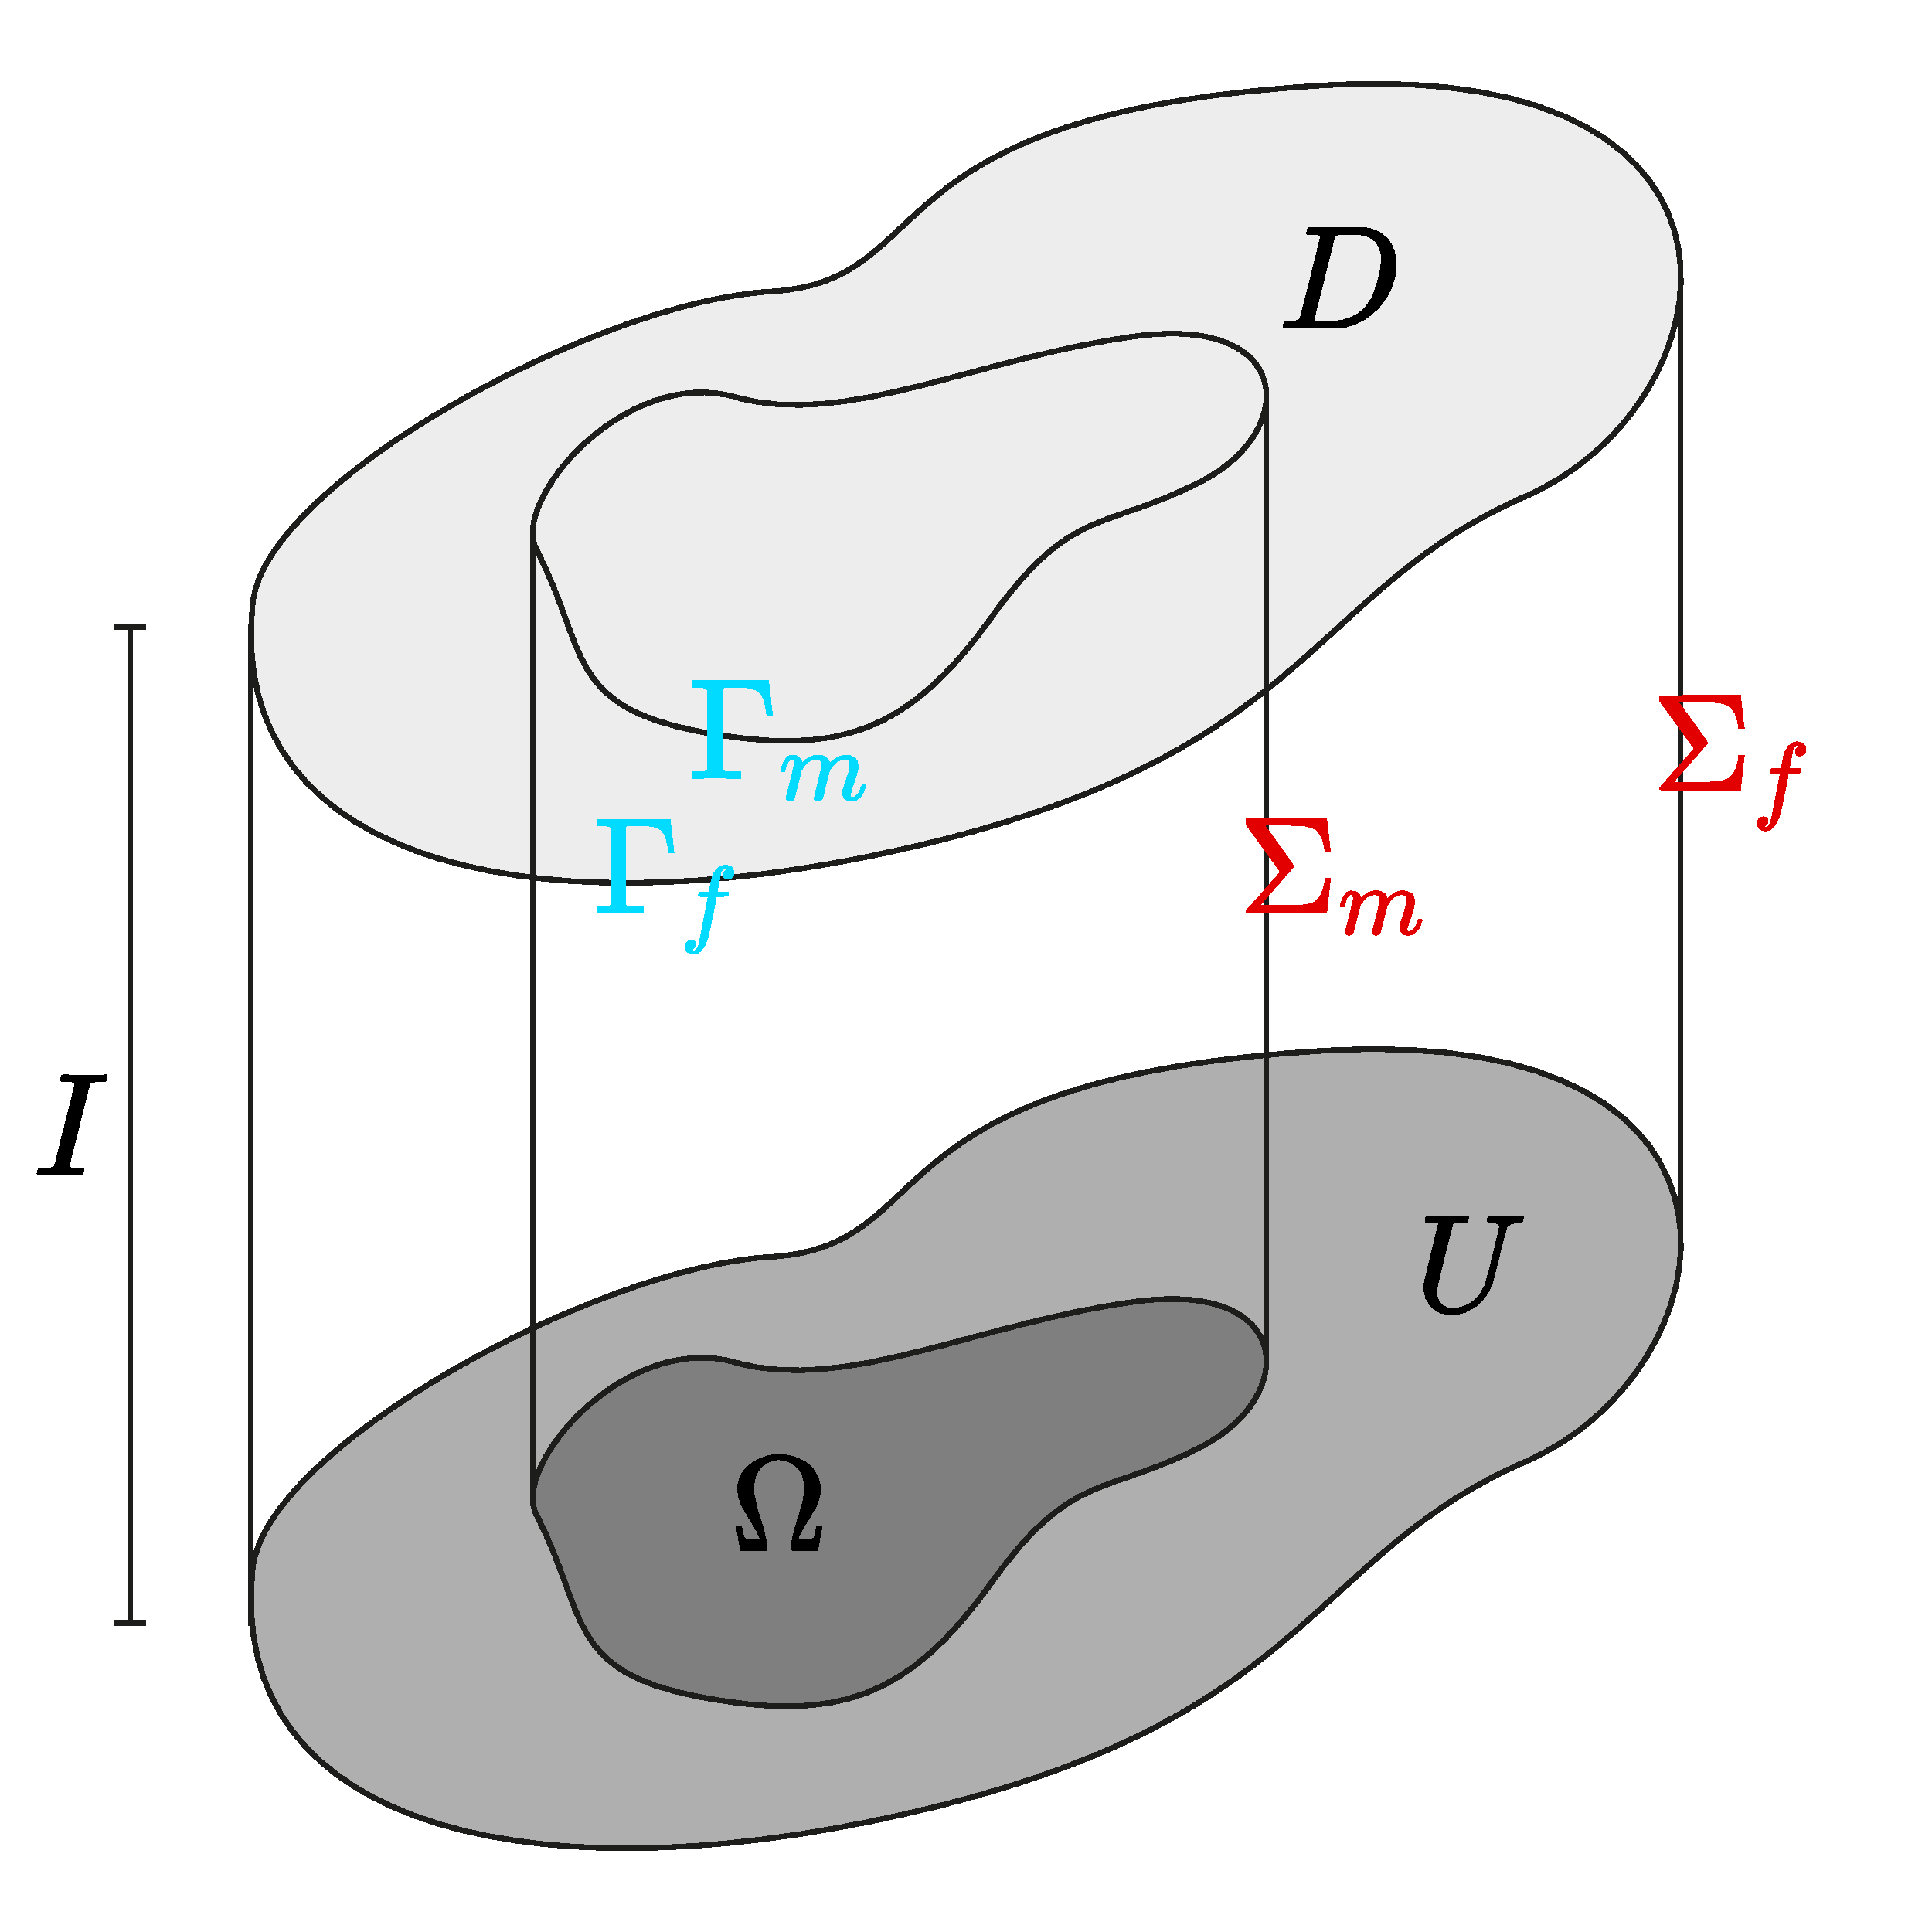
\includegraphics[height=0.35\columnwidth]{Images/Domains.pdf}
\caption{Space-time cylinder and 2D domain}\label{fig:space_time}
\end{figure}

Let us interpret $D$ as a uniform and isotropic body, inside of which an inclusion $\Omega$ of zero temperature is present (think of an ice cube submerged in water). The temperature $u$ inside $D\setminus \overline{\Omega} = U$ evolves over time according to the heat equation, at least approximately, and we are interested in obtaining the shape of the inclusion, which we suppose to be inaccessible, so that we cannot directly measure it. We are however allowed to access the outer boundary $\partial D$ and measure surface temperature and normal heat flux: we ask ourselves how to recover $\partial \Omega$ from the knowledge of this boundary data only. This is a non-linear and ill-posed inverse problem (according to e.g. \cite{harbrecht}). 

Summing up, our task is, given the outer temperature and heat flux, to reconstruct the shape of $\Omega$ that induced, through heat diffusion, those boundary quantities.

In more mathematical terms, let us consider a heat equation on the unknown cylinder $U\times I$, with zero initial condition and no volumetric forcing term, where on $\Sigma_f$ are prescribed smooth enough Dirichlet and Neumann data simultaneously (call them $f$ and $g$, they correspond to the outer temperature and heat flux), while on $\Sigma_m$, homogeneous Dirichlet conditions.

\begin{pb}[Overdetermined heat equation]
\label{pb:pdes}
Call $U:=D\setminus \overline{\Omega}$. We look for $u:U \times I \rightarrow \mR$ solving:
\begin{align*}
\left\{\begin{matrix}
u_t -\Delta u=0 & \text{on }U\times I \\ 
u(0)=0 & \\ 
u = f, \partial_\nu u=g & \text{on }\Sigma_f\\
u = 0 & \text{on }\Sigma_m\\
\end{matrix}\right.
\end{align*}

We introduce the splitting:

\begin{align*}
\begin{matrix}
\left\{\begin{matrix}
v_t -\Delta v=0 & \text{on }U\times I \\ 
v(0)=0 & \\ 
v = f& \text{on }\Sigma_f\\
v = 0 & \text{on }\Sigma_m\\
\end{matrix}\right. &, \quad  \left\{\begin{matrix}
w_t -\Delta w=0 & \text{on }U\times I \\ 
w(0)=0 & \\ 
\partial_\nu w=g & \text{on }\Sigma_f\\
w = 0 & \text{on }\Sigma_m\\
\end{matrix}\right.
\end{matrix}
\end{align*}
\end{pb}

It can be shown that, for arbitrary $f,g$, there exists at most one $\Omega$ such that \cref{pb:pdes} is solvable (see \cite{chapko1}, \cite{chapko2})

%, so that possessing measurements of the actual data $f$ and $g$ might allow us to reconstruct $\Omega$.

We can leverage this property to find a numerical approximation for such domain.
In particular, the equations for $v,w$ are always uniquely solvable, and $u=v$, $u=w$, in case $u$ exists, i.e. when the shape identification problem admits a solution. One way to find $\partial \Omega$ is therefore, given data $f,g$ and a guess $\hat{\Omega}$ of the sought domain, to simulate $v,w$ on $\hat{\Omega}$, measure their discrepancy $\norm{v-w}$ and use this knowledge to improve the iterate $\hat{\Omega}$ and get closer to the actual inclusion $\Omega$, by trying to minimize $\norm{v-w}$.

%\begin{figure}[H]
%\centering
%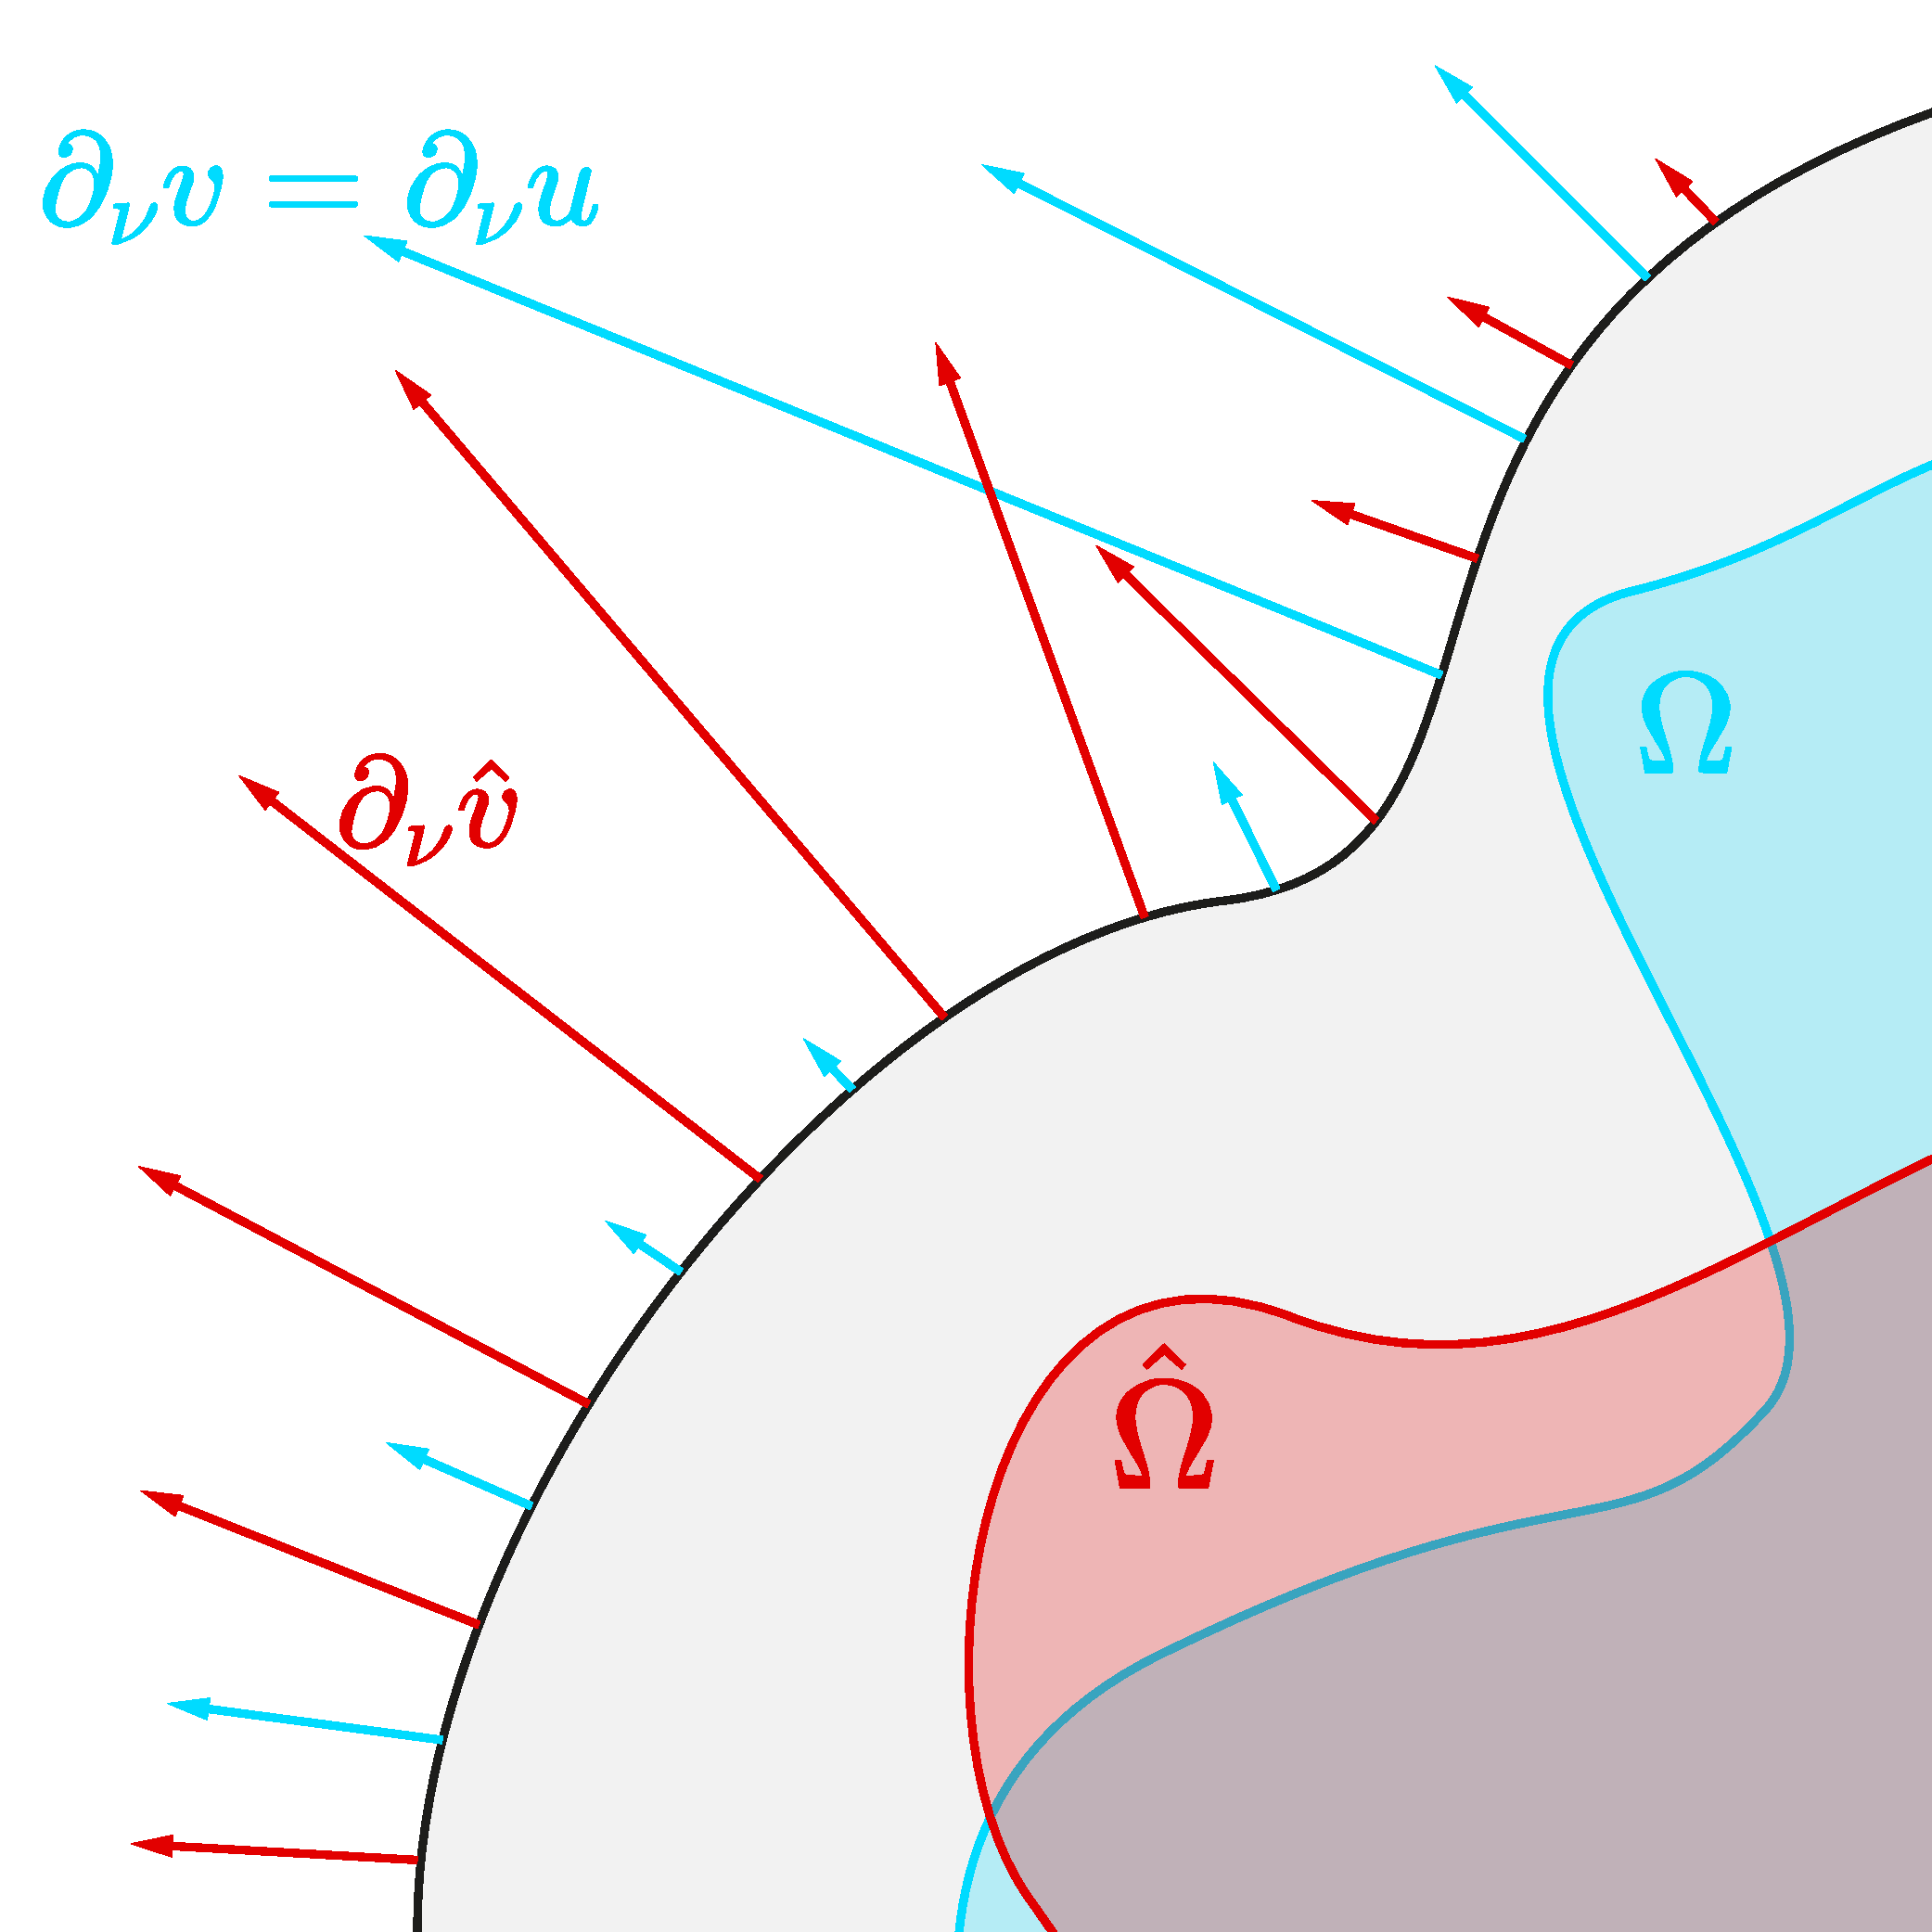
\includegraphics[width=0.25\columnwidth]{Images/NormalDiscrepancy.pdf}
%\caption{Discrepancy between the Neumann data corresponding to the correct domain $\Omega$, and a guess of it, $\hat{\Omega}$}\label{fig:normal_discrepancy}
%\end{figure}

So, the thesis revolves around the following problem.

\begin{pb}[Shape identification problem]
\label{pb:shid}
We aim at finding $\Omega$ such that $u$, defined in \cref{pb:pdes}, exists, i.e. such that $v=w$.
\end{pb}

This same problem was addressed in \cite{harbrecht} using a slightly different approach than ours, involving boundary integral equations, boundary element methods and non-standard time stepping schemes. On the other hand our focus has a rather ``volumetric" flavour, as we will discuss in the following chapters, and we make use of the well known implicit Euler or Crank-Nicolson algorithms.

As already mentioned, some uniqueness results for \cref{pb:shid} are already available. We are not concerned with the issue of the existence of $\Omega$, likewise this aspect is not addressed in the aforementioned work \cite{harbrecht}. Some advances in this direction were made in the case where $\Omega$ is allowed to evolve with time, see \cite{brugger}.

In the following we will formalize assumptions, setting and notation, and we will tackle \cref{pb:shid} by shape optimization techniques.

\section{Treatment by shape optimization}
\label{sec:shopt_treatment}

\begin{ass}[Geometry assumptions for the shape optimization problem]
\label{ass:geo_sh}
Let $D\subseteq \mR^n$, $\Omega_r \cc D$ be simply connected bounded Lipschitz domains, in the sense of \cite{grisvard}, definition 1.2.1.1. Define $U_r:=D\setminus \overline{\Omega_r}$, the so-called ``reference domain", which is also bounded and Lipschitz.
\end{ass}

Let us describe the set of admissible domains where $\Omega$ is a-priori searched. We follow the ``perturbation of identity" ansatz from \cite{murat}.

\begin{defn}[Admissible transformations]
\label{def:adm_transf}
Given $D$, we consider the set $\cT:=\{\tau:\mR^n\rightarrow\mR^n, \tau \text{ bi-Lipschitz}, \tau|_{D^c} = \id\}$, endowed with the ``perturbation space" $\Te:=\{ \delta \te \in W^{1,\infty}(\mR^n;\mR^n), \delta \te|_{D^c}=0\}$, see also \cref{def:adm}.

We will consider transformations of $U_r$ that belong to $\cT_a:=\cT \cap \{ \tau \in W^{1,\infty}(\mR^n, \mR^n), \norm{\tau - \id}_{W^{1,\infty}(\mR^n, \mR^n)}<C(U_r)\}$, where the presence of the bound by $C(U_r)$ is to ensure that $\tau(U_r)\cc D$ is also bounded Lipschitz, and the existence of such constant is guaranteed by \cref{thm:ptb_id_lip}.

\end{defn}

\begin{obs}[Smallness assumption]
\mbox{}\\
To carry out arguments with such a general form of tranformation $\tau$, an assumption of ``smallness" (such as the one involving $C(U_r)$) is necessary, to keep $\tau(U_r)$ Lipschitz. A more transparent way of ensuring that $\tau(U_r)\cc D$ is Lipschitz, can be found in \cref{sec:star}.
\mbox{}\\
Also note, that $\tau$ has a Lipschitz inverse yields $\tau(U_r)\cc D$: for $x \in D$, we have in fact $0<\delta = \inf_{d \in \partial D}|x-d|\leq \norm{\tau^{-1}}_{W^{1,\infty}(\mR^n,\mR^n)}\inf_{d \in \partial D}|\tau(x)-d|$.
\end{obs}

%We remark that there exists a unique Lipschitz continuous representive $T$ of $\tau \in \cT_a$ (see \cref{prop:lip}), and that we denote it also by $\tau$, for simplicity: by $\tau(U_r)$ we precisely mean $T(U_r)$.

We now recast \cref{pb:shid} into a new form, suitable for shape optimization, as done in \cite{harbrecht}. We mention that the equations for $v,w$ of \cref{pb:pdes} are well posed, this is discussed in detail in the appendices. We remark that, given any extension $\bar{u}$ of $f$ onto $U\times I$ (in the sense of \cref{prop:trace}), then $v$ decomposes as $v = v_0+\bar{u}$, where $v_0$ solves another heat equation with zero Dirichlet conditions. We therefore write $v^\tau = v_0^\tau + \bar{u}$ and $w^\tau$ to emphasize the dependence on $\tau$, and refer the reader to \cref{pb:mix}, \cref{pb:diri_ext} and \cref{pb:joint_mov} for additional details on the PDEs formulations.

\begin{pb}[Shape optimization problem]
\label{pb:shopt}
Suppose that \cref{ass:geo_sh}, \cref{ass:basic_par_mix} (applied to \cref{pb:pdes}) hold. We want to solve:

$$\inf_{\tau \in \cT_a}\frac{1}{2}\norm{v^\tau-w^\tau}_{L^2(I,H_\tau)}^2=:J(\tau)$$

The notation for the spaces also comes from  \cref{pb:joint_mov}: $\cdot_\tau$ means that the space is based on the moving domain $\tau(U_r)$, and $H=L^2, \tw{V}=H^1_0, \tw{W} = H^1_{0,m}=\{v \in H^1, v(\Gamma_m)=0\}$ (see also \cref{sec:pdes} for the last space), so that e.g. $H_\tau = L^2(\tau(U))$.

\end{pb}

Therefore, we are now concerned with finding a function $\tau$, instead of a generic set $\Omega$, and this way we can make use of functional analytic techniques and results from optimal control.

%\begin{obs}[Well-posedness of $J$]
%\mbox{}\\
%We know from the proof of \cref{thm:mix_reg} that $v_0^\tau + \bar{u}$ doesn't depend on the particular choice of $\bar{u}$, therefore, for different $\tau$ yielding the same domain $U$, $J(\tau)$ doesn't change.

%\end{obs}

\begin{obs}[Tracking type cost functional]
\mbox{}\\
We have chosen the distributed $L^2(I,L^2)$ norm to measure the discrepancy $v^\tau\simeq w^\tau$ on the whole $\tau(U_r)$. Apart from having favourable functional analytic properties (Fréchet differentiability, to mention one), such cost functional will also allow us to obtain ``better behaved" adjoint states. In fact, contrary to \cite{harbrecht}, the heat equations for the adjoint states (see \cref{prop:gateaux_diff}) will have better compatibility between initial condition and boundary conditions. This potentially simplifies the numerical analysis of such equations, as we will make clearer later on.
\end{obs}





Now, let $U:=\tau(U_r)$, for $\tau \in \cT_a$ and let $\delta \te \in \Te$. To find a better (in the sense of the energy $J$) candidate $\tau$ for the solution of \cref{pb:shopt}, we can use gradient information and perturb our current guess $\tau$ in the direction of steepest descent for $J$, a direction dictated by the (Gateaux) shape gradient $J'$ of $J$ (for more details on how to extract such direction, see \cref{sec:hilbert}). We are hence interested in finding $J'(\tau) \in \Te^*$ such that, for all $\delta \te \in \Te$:

$$\lim_{t \rightarrow 0 }\frac{|J(\tau+t\delta \te)-J(\tau)-t J'(\tau)[\delta \te]|}{t}=0$$

Spelled out differently, for all null sequences $t_k \rightarrow 0$, we must have:


$$\lim_{k}\frac{|J(\tau+t_k \delta \te)-J(\tau)-t_k J'(\tau)[\delta \te]|}{t_k}=0$$

%We have set $\norm{\te}_\Te = \norm{\te}_{W^{1,\infty}(\mR^n;\mR^n)}=\norm{\te}_{W^{1,\infty}(D;\mR^n)}$.

These two defitions of (Gateaux) shape gradient are equivalent, but we prefer the second one since in the proof of \cref{prop:gateaux_diff} we will be dealing with weak convergence, so that sequences arise naturally. The proof would also work with the first definition.

Note, also thanks to \cref{prop:ptb_id}, that for small $t_k$, e.g. for $k$ large enough, we have $\tau + t_k \delta \te \in \cT_a$.

%, yields an element $\tau +\delta  \te \in \cT_a$: it will be this the way in which an initial guess for the sought domain $\Omega = \tau(\Omega_r)$ will be refined, i.e. by iteratively adding to $\tau$, small perturbations $\delta \te$. 


%Note, $\tau+\delta \te_k \in \cT_a$ for large enough $k$. In fact, $\tau+\delta \te_k \in \cT$ for large $k$ as in \cref{prop:ptb_id}, and the condition on $C(U_r)$ is satisfied too, because $\te :=\tau-\id$ was already in the $W^{1,\infty}$ open ball of radius $C(U_r)$ centered at the origin, and so will be $\te + \delta_k\te$, always for large $k$.

Also, $\tau+t_k \delta \te  = (\id+t_k \delta\te \circ \tau^{-1})\circ \tau$, and $\id+t_k \delta\te \circ \tau^{-1}$ is in $\cT_a$ (also by \cref{prop:ptb_id} and the reasoning above). We are then equivalently interested in:

$$\lim_{k}\frac{|J((\id+t_k \delta\te \circ \tau^{-1})\circ \tau)-J(\tau)-t_k J'(\tau)[\delta \te]|}{t_k}$$

%This amounts to setting the reference domain to $\tau(U_r)$ instead of $U_r$ and perturbing the former, at least for the sake of computing derivatives.

We now introduce a ``Lagrangian" functional in order to derive the expression of the shape gradient $J'$ of $J$. There are several ways about this task in the literature (see e.g. \cite{avg_adj}, \cite{cea} or \cite{lindemann}), and we will adopt that contained in \cite{avg_adj}. It requires the PDEs corresponding to $\tau + t_k \delta \te$ to be all reformulated on the domain $\tau(U_r)$, where $\tau$ is exactly the evaluation point of $J'$. To find a transported formulation of our PDEs to a different domain, we need to consider the variational formulations of $v^{\tau + t_k \delta \te}$ and $w^{\tau+t_k \delta \te}$ and then apply a change of variables to the appearing integrals. This is precisely addressed \cref{thm:eq_pde} (whose applicability is ensured by \cref{ass:basic_par_mix} and by \cref{ass:pull}, which holds by \cref{ass:geo_sh}).

For $k$ large, i.e. $k\geq K(\tau)$, we have $\zeta_k:=\id+t_k \delta\te \circ \tau^{-1} \in \cT_a$, as seen above, and  having \cref{thm:eq_pde} in mind we can set:

\begin{align*}
L_\tau(k,w,v_0,q,p) := \\
\frac{1}{2}\int_I \int_{\tau(U_r)}|v_0+\bar{u} \circ \zeta_k - w|^2|\det(D\zeta_k)|+\\
\int_I ( w_t , q |\det(D\zeta_k)|)_{H_\tau}+ (A_{\zeta_k}\nabla w, \nabla q)_{H_\tau} -\int_I(g,\tr_{U} q)_{L^2(\Gamma_f)} +\\ \int_I (v_{0t},p |\det(D\zeta_k)|)_{H_\tau} + (A_{\zeta_k} \nabla v_0, \nabla p)_{H_\tau}+\int_I((\bar{u}\circ \zeta_k)',p|\det(D\zeta_k)|)_{H_\tau}+(A_{\zeta_k} \nabla (\bar{u} \circ \zeta_k), \nabla p)_{H_\tau}
\end{align*}

Here $w \in Q_0(I, \tw{W}_\tau), v_0 \in Q_0(I,\tw{V}_\tau), q \in Q^0(I, \tw{W}_\tau), p \in Q^0(I, \tw{V}_\tau)$, where the space $Q$ is thoroughly described after its introduction in \cref{def:Q}, which we recall: $Q(I,V)=H^{1,1}=L^2(I,V)\cap H^1(I,H)$, and $Q^0$ means the imposition of a zero terminal condition ($Q_0$ stands for zero initial condition). We have set $A_\tau:=  (D\tau)^{-1}(D\tau)^{-t}|\det(D\tau)|$.

$L_\tau$ is composed of three parts: the cost functional and the two variational formulation of $v_0^\tau$ and $w^\tau$, transported to the domain $\tau(U_r)$, which is fixed when computing the shape gradient.

Note that to be precise, $\bar{u}$ is any extension of the Dirichlet datum $f$ to the domain $I \times \zeta_k(\tau(U_r))$ (see \cref{prop:trace}, \cref{pb:diri_ext}). Because of this, let us fix $\bar{u}_\tau$, an extension of $f$ on $\tau(U_r)$ and choose $\bar{u}:=\bar{u}_\tau\circ \zeta_k^{-1}$, a legitimate extension of $f$.

%In particular:

%\begin{itemize}
%	\item composition with $\tau$ preserves the smoothness of the extension, as seen in \cref{lemma:bochner_Hk_map}, given that $\circ \zeta_k^{-1}$ is a linear bounded operator between $\tw{W}_\tau$ and $\tw{W}_{\zeta_k \circ \tau}$ (see \cref{thm:change})
%	\item the initial value is preserved, as seen in the proof of \cref{prop:change_boch}
%	\item the trace on $\Sigma_f$ is preserved, because the trace on $\Gamma_f=\partial D$ is preserved, see \cref{thm:change}
%\end{itemize}

Therefore, we can state the following definition.

\begin{defn}[Lagrangian]

For a fixed $\tau \in \cT_a$ and  $k\geq K(\tau)$, for $\zeta_k:=\id+t_k \delta\te \circ \tau^{-1} \in \cT_a$, we define:

\begin{align*}
L_\tau(k,w,v_0,q,p) = \\
\frac{1}{2}\int_I \int_{\tau(U_r)}|v_0+\bar{u}_\tau - w|^2|\det(D\zeta_k)|+\\
\int_I ( w_t , q |\det(D\zeta_k)|)_{H_\tau}+ (A_{\zeta_k}\nabla w, \nabla q)_{H_\tau} -\int_I(g,\tr_{U} q)_{L^2(\Gamma_f)} +\\ \int_I (v_{0t},p |\det(D\zeta_k)|)_{H_\tau} + (A_{\zeta_k} \nabla v_0, \nabla p)_{H_\tau}+\int_I(\bar{u}_\tau',p|\det(D\zeta_k)|)_{H_\tau}+(A_{\zeta_k} \nabla \bar{u}_\tau , \nabla p)_{H_\tau}
\end{align*}

$L_\tau$ is defined as a map $\{k\geq K(\tau)\}\times Q_0(I, \tw{W}_\tau)\times Q_0(I,\tw{V}_\tau)\times Q^0(I, \tw{W}_\tau)\times Q^0(I, \tw{V}_\tau)\rightarrow \mR$.

We call $u = (w,v_0)$, $\pi = (q,p)$ (states and adjoints), $G(k,u,\pi) = L_\tau(k,w,v_0,q,p)$ to ease the notation.

We also call $b(k, u) = \frac{1}{2}\ds\int_I \int_{\tau(U_r)}|v_0+\bar{u}_\tau - w|^2|\det(D\zeta_k)|$ and $a(k, u,\pi) = G(k,u,\pi)-b(k, u)$, $E = Q_0(I, \tw{W}_\tau)\times Q_0(I,\tw{V}_\tau)$, $F=Q^0(I, \tw{W}_\tau)\times Q^0(I, \tw{V}_\tau)$, the spaces for states and adjoints.

\end{defn}

The rest of this section is devoted to applying the averaged adjoint method \cite{avg_adj} to our problem, so as to identify the volume expression of the shape gradient $J'(\tau)$. To this end we will have to state some properties of the Lagrangian $L_\tau $, as required in \cite{avg_adj}.

\begin{prop}[Properties of the Lagrangian]
\label{prop:lagr}

$L_\tau$ satisfies the following properties:

\begin{enumerate}
	\item $\psi \mapsto a(k, \phi,\psi)$ is linear, no matter what $\phi,k$
	\item $G$ is Fréchet differentiable with respect to $\psi$ at $(k,\phi,0)$ for all $k, \phi$
	\item $d_\psi G(k,\phi,0)[\delta \psi]=0$ for all $\delta \psi \in F$, admits a unique solution $\phi = u^k$
	\item $[0,1]\ni s \mapsto G(k, su^k + (1-s)u^0,\psi)$ is in $AC[0,1]$, no matter what $k, \psi$
	\item $G$ is Fréchet differentiable with respect to $\phi$ at $(k,\psi,\phi)$ for all $k, \psi, \phi$
	\item $[0,1]\ni s \mapsto d_\phi G(k, su^k + (1-s)u^0,\psi)[\delta \phi]$ is in $L^1(0,1)$, no matter what $k, \psi, \delta \phi$
	\item there exists a unique solution $\psi = \pi^k$ to $\ds \int_0^1 d_\phi G(k, su^k + (1-s)u^0,\psi)[\delta \phi]ds =0$ for all $\delta \psi$ 
\end{enumerate}

In particular $\pi^k = (Q^k \circ \tau^k,P^k \circ \tau^k)$, where we introduced the averaged adjoint problems on $I\times (\zeta_k\circ \tau )(U_r)$:

\begin{pb}[Averaged adjoint equations]
\label{pb:avg_adj_pb}
\begin{align*}
\left\{\begin{matrix}
-Q^k_t-\Delta Q^k =\frac{v_0^k-w^k+v_0^0-w^0}{2}\circ \zeta_k^{-1}+\bar{u}_\tau\circ \zeta_k^{-1}  \text{ on } (\tau + t_k\delta \te)(U) \\
Q^k(T)=0\\
\partial_\nu Q^k = 0 \text{ on } \Sigma_f\\
Q^k = 0 \text{ on } \Sigma_{m,k}
\end{matrix}\right.
\end{align*}

\begin{align*}
\left\{\begin{matrix}
-P^k_t-\Delta P^k =-\frac{v_0^k-w^k+v_0^0-w^0}{2}\circ \zeta_k^{-1}-\bar{u}_\tau\circ \zeta_k^{-1} \text{ on } (\tau + t_k\delta \te)(U)\\
P^k(T)=0\\
P^k = 0 \text{ on } \Sigma_f\\
P^k = 0 \text{ on } \Sigma_{m,k}
\end{matrix}\right.
\end{align*}
\end{pb}

\end{prop}

\begin{mproof}

We give some comments for the non trivial points.

%\underline{Proof of 2}
%
%All the pieces are linear in $\psi$. We only check the boundedness of the various differentials. For simplicity, call $|\det(D\zeta_k)|=d$, and note that   $\norm{qd}_{H_\tau}\leq C(d)\norm{q}_{H_\tau}$.
%
%And now, for instance:
%%\int_I \langle w_t , q |\det(DT_\e)|\rangle_{V^*_T,V_T}+ (A_{T_\e}\nabla w, \nabla q)_{H_T} -\int_I(g,\tr_{U} q)_{L^2(\Gamma_f)}
%\begin{align*}
%\int_I ( w_t , \delta q |\det(D\zeta_k)|)_{H_\tau} = \int_I ( w_t , \delta q d )_{H_\tau}\leq\\ C(d) \int_I \norm{w_t}_{H_\tau}\norm{\delta q}_{H_\tau}\leq C(d) \norm{w_t}_{L^2(I,H_\tau)}\norm{\delta q}_{L^2(I,H_\tau)}\leq\\C(d) \norm{w}_{Q(I,\tw{W}_\tau)}\norm{\delta q}_{Q(I,\tw{W}_\tau)}\leq
%C(d) \norm{w}_{Q(I,\tw{W}_\tau)}(\norm{\delta q}_{Q(I,\tw{W}_\tau)}+\norm{\delta p}_{Q(I,\tw{W}_\tau)}) =\\ C(d) \norm{w}_{Q(I,\tw{W}_\tau)}\norm{\delta\psi}_F
%\end{align*}
%
%Or also:
%
%\begin{align*}
%\int_I(g,\tr_{U} \delta q)_{L^2(\Gamma_f)}\leq \int_I \norm{g}_{L^2(\Gamma_f)}\norm{\delta q}_{\tw{W}_\tau}\leq \norm{g}_{H^1(I,L^2(\Gamma_f))}\norm{\delta\psi}_F
%\end{align*}
%
%and:
%
%\begin{align*}
%\int_I (A_{\zeta_k} \nabla \bar{u}_\tau, \nabla\delta p)_{H_\tau}\leq C\norm{A_{\zeta_k}}_{L^\infty(D;\mR^{n\times n})}\int_I \norm{\nabla \bar{u}_\tau}_{L^2(I,H_\tau)}\norm{\nabla\delta p}_{L^2(I,H_\tau)}\leq\\ C(\tau) \norm{\delta\psi}_F \norm{\bar{u}}_{H^1(I,\tw{W}_\tau)}
%\end{align*}

\underline{Proof of 3}

Testing $d_\psi G(k,\phi,0)[\delta \psi]=$ separately with $\delta \psi =(\delta q, 0)$ and $\delta \psi = (0,\delta p)$ we get back the state equations, so that a unique solution exists by \cref{thm:eq_pde} and \cref{thm:mix_reg}.
%
%\underline{Proof of 4}
%
%Every piece but $b$ is linear or constant in the state $\phi$. We only need to prove that $[0,1]\ni s \mapsto b(k, su^k + (1-s)u^0)$ is $AC[0,1]$. But by the structure of the cost function $J$, transported on $\tau(U_r)$, we see that the latter is a quadratic polynomial in $s$, hence, absolutely continuous.

%\underline{Proof of 5}
%
%For the pieces with the gradients, it follows as above, by in case employing the simmetry of $A_{\zeta_k}$.
%
%Now, for instance the linear form $\delta v_0 \mapsto \int_I (\delta v_{0t},p |\det(D\zeta_k)|)_{H_\tau}$ is also bounded by $C(d) \norm{\delta v_0}_{Q(I,\tw{V}_\tau)}\norm{\delta q}_{Q(I,\tw{W}_\tau)}$ just like before.
%
%What remains to check is the Fréchet differentiability of $b$.
%
%To do so, perturb $\phi$ by $\delta \phi$ and expanding the square:
%
%\begin{align*}
%\frac{1}{2}\int_I \int_{\tau(U_r)}|v_0+\delta v_0+\bar{u}_\tau - w-\delta w|^2|\det(D\zeta_k)| = \\\frac{1}{2}\int_I \int_{\tau(U_r)}|v_0+\bar{u}_\tau - w|^2|\det(D\zeta_k)|+\\\frac{1}{2}\int_I \int_{\tau(U_r)}|\delta v_0-\delta w|^2|\det(D\zeta_k)|+\\\int_I \int_{\tau(U_r)}(v_0+\bar{u}_\tau - w)(\delta v_0-\delta w)|\det(D\zeta_k)|
%\end{align*} 
%
%Now, $\ds \int_I \int_{\tau(U_r)}|\delta v_0-\delta w|^2|\det(D\zeta_k)|\leq C(\zeta_k)\norm{\delta v_0-\delta w}_{L^2(I,H_\tau)}^2\leq C(\zeta_k)\norm{\phi}_E^2$, so that this term is of higher term.
%
%And $\ds \int_I \int_{\tau(U_r)}(v_0+\bar{u}_\tau - w)(\delta v_0-\delta w)|\det(D\zeta_k)|$ is linear and bounded by reasonings similar to the former ones.
%
%\underline{Proof of 6}
%
%By the last point:
%
%\begin{align*}
%d_\phi G(k, \phi ,\psi)[\delta \phi] =\\
%\int_I ((v_0+\bar{u}_\tau - w)|\det(D\zeta_k)|,\delta v_0-\delta w)_{H_\tau}+\\
%\int_I (\delta w_t , q |\det(D\zeta_k)|)_{H_\tau}+ (A_{\zeta_k}\nabla \delta w, \nabla q)_{H_\tau}+\\
%\int_I (\delta v_{0t},p |\det(D\zeta_k)|)_{H_\tau} + (A_{\zeta_k} \nabla \delta v_0, \nabla p)_{H_\tau}
%\end{align*}
%
%so that:
%
%\begin{align*}
%d_\phi G(k, su^k + (1-s)u^0,\psi)[\delta \phi] = \\
%\int_I ((s(v_0^k+\bar{u}_\tau - w^k)+(1-s)(v_0^0+\bar{u}_\tau - w^0))|\det(D\zeta_k)|,\delta v_0-\delta w)_{H_\tau}+\\
%\int_I ( \delta w_t , q |\det(D\zeta_k)|)_{H_\tau}+ (A_{\zeta_k}\nabla \delta w, \nabla q)_{H_\tau}+\\
%\int_I ( \delta v_{0t},p |\det(D\zeta_k)|)_{H_\tau} + (A_{\zeta_k} \nabla \delta v_0, \nabla p)_{H_\tau}
%\end{align*}
%
%which is a degree $1$ polynomial in $s$, hence, $L^1(0,1)$.

\underline{Proof of 7}

It is readily seen that:

\begin{align*}
\int_0^1d_\phi G(k, su^k + (1-s)u^0,\psi)[\delta \phi]ds = \\
\int_I (((v_0^k+\bar{u}_\tau - w^k)+(v_0^0+\bar{u}_\tau - w^0))/2|\det(D\zeta_k)|,\delta v_0-\delta w)_{H_\tau}+\\
\int_I ( \delta w_t , q |\det(D\zeta_k)|)_{H_\tau}+ (A_{\zeta_k}\nabla \delta w, \nabla q)_{H_\tau}+
\int_I ( \delta v_{0t},p |\det(D\zeta_k)|)_{H_\tau} + (A_{\zeta_k} \nabla \delta v_0, \nabla p)_{H_\tau} = ...
\end{align*}

We get $ \delta w_t  = (\delta w\circ \zeta_k^{-1})_t\circ \zeta_k$, where $\delta w\circ \zeta_k^{-1} \in Q_0(I,\tw{W}_{\zeta_k \circ \tau})$ by \cref{prop:change_boch}.
Applying a change of variables we are left with:

\begin{align*}
... = \int_I \left (\frac{v_0^k-w^k}{2}\circ \zeta_k^{-1}+ \frac{v_0^0-w^0}{2}\circ \zeta_k^{-1}+\bar{u}_\tau\circ \zeta_k^{-1} ,\delta v_0\circ \zeta_k^{-1}-\delta w\circ \zeta_k^{-1}\right)_{H_{\zeta_k \circ \tau}}+\\
\int_I ((\delta w\circ \zeta_k^{-1})_t , q\circ \zeta_k^{-1} )_{H_{\zeta_k \circ \tau}}+ (\nabla (\delta w\circ \zeta_k^{-1}), \nabla( q\circ \zeta_k^{-1}))_{H_{\zeta_k \circ \tau}}+\\
\int_I ( (\delta v_{0}\circ \zeta_k^{-1})_t,p \circ \zeta_k^{-1})_{H_{\zeta_k \circ \tau}} + ( \nabla \delta (v_0\circ \zeta_k^{-1}), \nabla (p\circ \zeta_k^{-1}))_{H_{\zeta_k \circ \tau}}
\end{align*}

Here, as we saw in \cref{prop:change_boch}, we have $\delta w\circ \zeta_k^{-1}, w\circ \zeta_k^{-1} \in Q_0(I, \tw{W}_{\zeta_k \circ \tau})$, $ \delta v_{0}\circ \zeta_k^{-1}, v_{0}\circ \zeta_k^{-1} \in Q_0(I,\tw{V}_{\zeta_k \circ \tau})$, $q\circ \zeta_k^{-1}\in Q^0(I, \tw{W}_{\zeta_k \circ \tau})$ and $p\circ \zeta_k^{-1}\in Q^0(I, \tw{V}_{\zeta_k \circ \tau})$.

Because $\circ \zeta_k^{-1}$ is a bijection of $Q_0(I,\tw{V}_{\zeta_k \circ \tau})$ and $Q_0(I,\tw{V}_{\zeta_k})$ by, again, \cref{prop:change_boch} (and analogously for $\tw{W}$), we have that  $\int_0^1 d_\phi G(k, su^k + (1-s)u^0,\psi)[\delta \phi]ds=0$ for all $\delta \phi \in E$ if and only if:

\begin{align*}
\int_I \left (\frac{v_0^k+w^k}{2}\circ \zeta_k^{-1}- \frac{v_0^0+w^0}{2}\circ \zeta_k^{-1}+\bar{u}_\tau\circ \zeta_k^{-1} ,\delta V_0-\delta W\right)_{H_{\zeta_k \circ \tau}}+\\
\int_I ( \delta W_t , q\circ \zeta_k^{-1})_{H_{\zeta_k \circ \tau}}+ (\nabla\delta W, \nabla( q\circ \zeta_k^{-1}))_{H_{\zeta_k \circ \tau}}+
\int_I ( \delta V_{0t},p \circ \zeta_k^{-1})_{H_{\zeta_k \circ \tau}} + ( \nabla \delta V_0, \nabla (p\circ \zeta_k^{-1}))_{H_{\zeta_k \circ \tau}} = 0
\end{align*}

for all $\delta W \in Q_0(I, \tw{W}_{\zeta_k \circ \tau})$, $ \delta V_{0} \in Q_0(I,\tw{V}_{\zeta_k \circ \tau})$.

We wish to find a (unique) solution $(q^k, p^k) \in Q^0(I, \tw{W}_\tau)\times Q^0(I, \tw{V}_\tau)$ of this problem. We can equivalently (by \cref{prop:change_boch}) find $(Q^k, P^k) \in Q^0(I, \tw{W}_{\zeta_k \circ \tau})\times Q^0(I, \tw{V}_{\zeta_k \circ \tau})$ satisfying:

\begin{align*}
\int_I \left (\frac{v_0^k-w^k}{2}\circ \zeta_k^{-1}+ \frac{v_0^0-w^0}{2}\circ \zeta_k^{-1}+\bar{u}_\tau\circ \zeta_k^{-1} ,\delta V_0-\delta W\right)_{H_{\zeta_k \circ \tau}}+\\
\int_I (\delta W_t ,Q^k )_{H_{\zeta_k \circ \tau}}+ (\nabla \delta W, \nabla Q^k)_{H_{\zeta_k \circ \tau}}+
\int_I( \delta V_{0t},P^k)_{H_{\zeta_k \circ \tau}} + ( \nabla \delta V_0, \nabla P^k)_{H_{\zeta_k \circ \tau}} = 0
\end{align*}

for all $\delta W, \in Q_0(I, \tw{W}_{\zeta_k \circ \tau})$, $ \delta V_{0} \in Q_0(I,\tw{V}_{\zeta_k \circ \tau})$.

Upon testing first with $\delta W=0$ and then with $\delta V_0=0$, an application of integration by parts in time (see \cref{prop:Q}) yields the problems which are the weak formulations (cfr. \cref{thm:eq_pde}, \cref{pb:mix} and \cref{pb:mix}) of the PDEs:

\begin{align*}
\begin{matrix}
\left\{\begin{matrix}
-Q^k_t-\Delta Q^k =\frac{v_0^k-w^k+v_0^0-w^0}{2}\circ \zeta_k^{-1}+\bar{u}_\tau\circ \zeta_k^{-1} \\
Q^k(T)=0\\
\partial_\nu Q^k = 0 \text{ on } \Sigma_f\\
Q^k = 0 \text{ on } \Sigma_{m,k}
\end{matrix}\right.
, \quad &
\left\{\begin{matrix}
-P^k_t-\Delta P^k =-\frac{v_0^k-w^k+v_0^0-w^0}{2}\circ \zeta_k^{-1}-\bar{u}_\tau\circ \zeta_k^{-1} \\
P^k(T)=0\\
P^k = 0 \text{ on } \Sigma_f\\
P^k = 0 \text{ on } \Sigma_{m,k}
\end{matrix}\right.
\end{matrix}
\end{align*}

Applying the time reversal $t\mapsto T -t$ (where $I = (0,T)$), these are a couple of standard heat equations for which we have available existence, uniqueness and stability results (see \cref{chap:parab_eq}, and \cref{thm:mix_reg}).

By calling then $\pi^k = (Q^k \circ \tau^k,P^k \circ \tau^k)$ we conclude the proof.
\end{mproof}

We now turn to the verification of Gateaux differentiability of $J$, applying the techniques proposed in \cite{avg_adj}.

\begin{prop}[Averaged adjoint method for Gateaux derivatives]
\label{prop:adv_adj}

Let $\delta \te \in \Te$. If $J'(\tau) \in \Te^*$ satisfies

$$\lim_{k}\frac{G(k,u^0,\pi^k)-G(0,u^0,\pi^k)}{t_k}=J'(\tau)[\delta \te]$$

then $J'(\tau)$ is the Gateaux derivative of $J$ at $\tau$.

\end{prop}

\begin{mproof}

See theorem 3.1, \cite{avg_adj}.
\end{mproof}

\begin{prop}[Gateaux differentiability of $J$]
\label{prop:gateaux_diff}
Given $\tau \in \cT_a$, $J$ is Gateaux differentiable at $\tau$ with respect to the $W^{1,\infty}$ topology. The Gateaux differential is:


\begin{align*}
J'(\tau)[\delta \te] =\\ \int_I (w_t^\tau \dive(\delta \te\circ  \tau^{-1}), q^\tau )_{L^2(\tau(U_r))}+ \int_I (A'(\delta\te \circ \tau^{-1})\nabla v^\tau, \nabla p^\tau)_{L^2(\tau(U_r))}+\\
\int_I (v_t^\tau \dive(\delta \te\circ  \tau^{-1}), p^\tau )_{L^2(\tau(U_r))}+ \int_I (A'(\delta\te \circ \tau^{-1})\nabla w^\tau, \nabla q^\tau)_{L^2(\tau(U_r))}+\\
\frac{1}{2}\int_I\int_{\tau(U_r)}|v^\tau-w^\tau|^2\dive(\delta \te\circ  \tau^{-1})
\end{align*}

where $p^\tau$, $q^\tau$ solve:

\begin{align*}
\begin{matrix}
\left\{\begin{matrix}
-q^\tau_t-\Delta q^\tau =v^\tau-w^\tau \text{ on } I \times \tau(U_r)\\
q^\tau(T)=0\\
\partial_\nu q^\tau = 0 \text{ on } \Sigma_f\\
q^\tau = 0 \text{ on } \Sigma_m
\end{matrix}\right., \quad & \left\{\begin{matrix}
-p^\tau_t-\Delta p^\tau = - v^\tau+ w^\tau  \text{ on } I \times \tau(U_r)\\
p^\tau(T)=0\\
p^\tau = 0 \text{ on } \Sigma_f \\
p^\tau = 0 \text{ on } \Sigma_m
\end{matrix}\right.
\end{matrix}
\end{align*}

and where $A'(\delta\te )= - D\delta \te -(D\delta\te)^t + \dive(\delta\te)I$.

\end{prop}

\begin{mproof}

\underline{The shape derivative is linear and bounded}

Linearity is immediate. For the boundedness, with $C$ independent of $\delta \te$, $\tau$:

\begin{align*}
|J'(\tau)[\delta \te]| \leq C \left ( \norm{\dive(\delta \te\circ  \tau^{-1})}_{L^\infty(\tau(U_r))}+\left(\sum_{ij} \norm{(A'(\delta\te \circ \tau^{-1})_{ij}}_{L^\infty(\tau(U_r))}\right )\right )\leq
C\norm{\delta \te }_{W^{1,\infty}(\mR^n;\mR^n)}
\end{align*}

where in the last step we applied \cref{prop:22416}. 

\underline{Conclusion}

Assume at first that $p^k \weakc p^0$ in $Q(I,\tw{V}_\tau)$ and $q^k \weakc q^0$ in $Q(I,\tw{W}_\tau)$, something which will be later verified. Using that $u^0=(w^\tau, v_0^\tau)$, and cancelling the boundary integrals:

\begin{align*}
G(k,u^0,\pi^k)-G(0,u^0,\pi^k) =\\
\frac{1}{2}\int_I \int_{\tau(U_r)}|v^\tau-w^\tau|^2(|\det(D\zeta_k)|-1)+\\
\int_I ( w_t^\tau (|\det(D\zeta_k)| -1), q^k)_{H_\tau}+ ((A_{\zeta_k}-I)\nabla w^\tau, \nabla q^k)_{H_\tau}+\\
\int_I (v_t^\tau (|\det(D\zeta_k)|-1),p^k )_{H_\tau} + ((A_{\zeta_k}-I) \nabla v^\tau, \nabla p^k)_{H_\tau} 
\end{align*}

Now, the application $\delta \te \mapsto \id +\delta \te \circ \tau^{-1}$ is Fréchet differentiable at $\delta \te =0$, as a map of $\Te$ into $\cV^1$ (see \cref{defn:spaces_trans}), with Fréchet derivative $\delta \te \circ \tau^{-1}$, which is linear and bounded in $\delta \te$ by \cref{prop:22416}.
% Note, we needed here $\tau \in \cT^1$.

Also, the maps $\delta \eta \mapsto |\det(D\eta)|$ and $\eta\mapsto (D\eta)^{-1}(D\eta)^{-t}|\det D\eta|$ are Fréchet differentiable at $\id$, from $\cV^1$ into $L^\infty(\mR^n;\mR)$ and $L^\infty(\mR^n;\mR^{n\times n})$, as stated in lemma 4.16, page 80 of \cite{lindemann}. Their Fréchet derivatives are $\dive (\beta)$ and $I-D\beta-(D\beta)^t$, respectively.

Therefore, composition with  $\delta \te  \mapsto \id+ \delta \te \circ \tau^{-1}$ yields two Fréchet differentiable maps whose derivatives at $0$, in direction $\delta \te \in \Te$, are exactly $\dive(\delta \te \circ \tau^{-1})$ and $A'(\delta \te \circ \tau^{-1})$, so that:

\begin{itemize}
	\item $|\det(D\zeta_k)|-1 = |\det(D\zeta_k)|-1 - t_k\dive(\delta \te \circ \tau^{-1})+t_k\dive(\delta \te \circ \tau^{-1}) = o^1_k + t_k\dive(\delta \te \circ \tau^{-1})$
	\item $A_{\zeta_k}-I = A_{\zeta_k}-I - t_k A'(\delta \te \circ \tau^{-1}) + t_k A'(\delta \te \circ \tau^{-1}) = o_k^2 + t_k A'(\delta \te \circ \tau^{-1}) $
\end{itemize}

where $o^1_k \in L^\infty(\mR^n;\mR)$ and $o^2_k \in L^\infty(\mR^n;\mR^{n\times n})$ are higher order terms, in $L^\infty$ and with respect to $t_k$. We can then write $(G(k,u^0,\pi^k)-G(0,u^0,\pi^k))/t_k = a_k + o_k$.

Here:

\begin{align*}
a_k :=
\frac{1}{2}\int_I \int_{\tau(U_r)}|v^\tau-w^\tau|^2\dive(\delta \te \circ \tau^{-1})+\\
\int_I ( w_t^\tau \dive(\delta \te \circ \tau^{-1}), q^k)_{H_\tau}+ (A'(\delta \te \circ \tau^{-1}) \nabla w^\tau, \nabla q^k)_{H_\tau}+\\
\int_I (v_t^\tau \dive(\delta \te \circ \tau^{-1}),p^k )_{H_\tau} + (A'(\delta \te \circ \tau^{-1})  \nabla v^\tau, \nabla p^k)_{H_\tau} 
\end{align*}

Thanks to the assumed weak convergence, $a_k\rightarrow J'(\tau)[\delta \te]$. So, we still have to show that:

\begin{align*}
o_k:=
\frac{1}{2}\int_I \int_{\tau(U_r)}|v^\tau-w^\tau|^2 o^1_k t_k^{-1}+\\
\int_I ( w_t^\tau o^1_kt_k^{-1}, q^k)_{H_\tau}+ (t_k^{-1}o^2_k\nabla w^\tau, \nabla q^k)_{H_\tau}+\\
\int_I (v_t^\tau o^1_k t_k^{-1},p^k )_{H_\tau} + (t_k^{-1}o^2_k \nabla v^\tau, \nabla p^k)_{H_\tau} 
\end{align*}

goes to zero. This is true thanks to the boundedness of the averaged adjoint states, which stems from their weak convergence, and the properties of $o_k^1,o_k^2$.


\underline{Weak convergence of states}

We assumed $p^k \weakc p^0$ in $Q(I,\tw{V}_\tau)$ and $q^k \weakc q^0$ in $Q(I,\tw{W}_\tau)$. We now prove these claims. We show at first  $v_0^k \weakc v^0_0$ in $Q(I,\tw{V}_\tau)$ and $w^k \weakc w^0$ in $Q(I,\tw{W}_\tau)$. We do this by uniformly estimating these quantities on $k$. To do this, we use the equations of $V_0^k:=v_0^k\circ \zeta_k^{-1}$ and $W^k:=w^k\circ \zeta_k^{-1}$ (see \cref{thm:eq_pde}) and \cref{thm:mix_reg}, to obtain the stability estimates:

\begin{align*}
\norm{V^k}^2_{C([0;T],H_{\zeta_k\circ \tau})}+\norm{V^k}_{L^2(I,H_{\zeta_k\circ \tau})}^2+ \norm{\nabla V^k}_{L^2(I,H_{\zeta_k\circ \tau})}^2 + \norm{(V^k)_t}^2_{L^2(I,H_{\zeta_k\circ \tau})}\leq C\norm{U^k}_{H^1(I,\tw{W}_{\zeta_k\circ \tau})}^2\\
\norm{W^k}^2_{C([0;T],H_{\zeta_k\circ \tau})}+\norm{W^k}_{L^2(I,H_{\zeta_k\circ \tau})}^2+ \norm{\nabla W^k}_{L^2(I,H_{\zeta_k\circ \tau})}^2 + \norm{W^k_t}^2_{L^2(I,H_{\zeta_k\circ \tau})}\leq C\norm{g}_{H^1(I,L^2(\Gamma_f))}^2
\end{align*}


where $C$ is independent of $k$.

%But $\norm{U^k}_{H^1(I,V_{T_k\circ T})}^2 = \norm{\bar{u}\circ T_k^{-1}}_{H^1(I,V_{T_k\circ T})}^2\leq N_k\norm{\bar{u}}_{H^1(I,V_{ T})}^2$ by \cref{lemma:bochner_Hk_map}, where $N_k:=\norm{\circ T_k}_{L(V_{T_k\circ T},V_{T}))}$.

Now, consider \cref{thm:change}. It says that for almost every time:

\begin{align*}
\norm{U^k}_{\tw{W}_{\zeta_k\circ \tau}}\leq \left ( 1+\norm{\det D\zeta_k}_{L^\infty(\mR^n)}\right)^{1/2} \norm{(D\zeta_k)^{-1}}_{L^\infty(\mR^n;\mR^{n\times n})}\norm{\bar{u}}_{H^1(\tau(U_r));\mR^n)}
\end{align*}

and a similar estimate we have for the first derivative. This bound is uniform on $k$ by \cref{prop:22416}.

We conclude that $\norm{U^k}_{H^1(I,\tw{W}_{\zeta_k\circ \tau})}^2$ is bounded and we thus have that $W^k \in Q_0(I, \tw{W}_{\zeta_k\circ \tau}), V_0^k \in Q_0(I,\tw{V}_{\zeta_k\circ \tau})$ are bounded.

Now, for almost all times, using \cref{thm:change}, we obtain that, for instance:
%4.11, page IV.6 of \cite{murat}
\begin{align*}
\norm{v_0^k}_{\tw{W}_{ \tau}}\leq \left ( 1+\norm{\det (D\zeta_k)^{-1}}_{L^\infty(\mR^n)}\right)^{1/2} \norm{D\zeta_k}_{L^\infty(\mR^n;\mR^{n\times n})}\norm{V_0^k}_{H^1(\zeta_k(\tau(U_r)))}
\end{align*}

where we remark that $H^1_0$ is chosen to be normed with the full $H^1$ norm.

The same goes for $w^k$ and the first derivatives in time, yielding that $w^k \in Q_0(I, \tw{W}_{ \tau}), v_0^k \in Q_0(I,\tw{V}_{\tau})$ are bounded.

We thus have $w^k\weakc w^? \in Q_0(I, \tw{W}_{ \tau})$, $v_0^k \weakc v_0^? \in Q_0(I,\tw{V}_{\tau})$, in the weak topologies of, respectively, $Q(I, \tw{W}_{ \tau}), Q(I,W_{\tau})$, and modulo subsequences. The initial values are preserved because $Q_0$ is closed and convex in the Hilbert space $Q$ (see also \cref{prop:Q}). 
%The closedness follows from the fact that the embedding into continuous function is linear bounded, and evaluation at $0$ is linear bounded from continuous functions.

We now prove that $w^?=w^0$, $v^?=v^0$, and this will yield the weak convergence of the whole sequence.
To prove e.g. that $v^?=v^0$, let us look at the weak formulations of $v_0^k$:

\begin{align*}
\int_I (v_{0t}^k,p |\det(D\zeta_k)|)_{H_\tau} + (A_{\zeta_k} \nabla v_0^k, \nabla p)_{H_\tau}+(\bar{u}',p|\det(D\zeta_k)|)_{H_\tau}+(A_{\zeta_k} \nabla \bar{u} , \nabla p)_{H_\tau} = 0
\end{align*}

for all $p \in Q_0(I,\tw{V}_{\tau})$.

Let's analyize the first term, which is $\ds \int_I (v_{0t}^k,p |\det(D\zeta_k)|)_{H_\tau} ) =(v_{0t}^k,p |\det(D\zeta_k)|)_{L^2(I,H_\tau)}$.
We can write:

\begin{align*}
(v_{0t}^k,p |\det(D\zeta_k)|)_{L^2(I,H_\tau)} = (v_{0t}^k,p )_{L^2(I,H_\tau)} + (v_{0t}^k,p (|\det(D\zeta_k)|-1))_{L^2(I,H_\tau)}
\end{align*}

Because $p \in  Q(I,\tw{V}_{\tau})$, the first term converges to $(v_{0t}^?,p )_{L^2(I,H_\tau)}$. The other term can be estimated as follows:
%, see \cref{prop:Q} for details on why we can write the time derivative of the limit

\begin{align*}
|(v_{0t}^k,p (|\det(D\zeta_k)|-1))_{L^2(I,H_\tau)}|\leq\norm{v_{0t}^k}_{L^2(I,H_\tau)}\norm{p }_{L^2(I,H_\tau)} \norm{|\det(D\zeta_k)|-1}_{L^\infty}
\end{align*}

where the first term in the product is bounded by the weak convergence property, and the last one goes to $0$ by continuity, see again \cref{prop:22416}. 
In a similar fashion for the other pieces, and by passing to the limit:
\begin{align*}
\int_I (v_{0t}^?,p)_{H_\tau} + (\nabla v_0^?, \nabla p)_{H_\tau}+(\bar{u}',p)_{H_\tau}+(\nabla \bar{u} , \nabla p)_{H_\tau} = 0
\end{align*}

so that $v^?=v^0$.

\underline{Weak convergence of averaged adjoint states}

So, $v_0^k \weakc v_0^0, w^k\weakc w^0$ in $Q(I,\tw{V}_\tau)$ and $Q(I,\tw{W}_\tau)$.
We now claim that $p^k \weakc p^0, q^k\weakc q^0$, and prove this similarly to before. We bound $P^k:=p^k\circ \zeta_k^{-1}$ and $Q^k:=q^k\circ \zeta_k^{-1}$.
By \cref{thm:const_track}, we will obtain a bound in $Q$  as soon as we have a bound on $\ds \frac{v_0^k-w^k+v_0^0-w^0}{2}\circ \zeta_k^{-1}$ in the $L^2(I,H)$ norm, and of $U^k:=\bar{u}_\tau\circ \zeta_k^{-1}$. The latter was proven above.

So, by \cref{thm:change} and \cref{prop:22416}, it suffices to have an $L^2(I,L^2)$ bound on $\ds \frac{v_0^k+w^k+v_0^0+w^0}{2}\circ \zeta_k^{-1}\circ \zeta_k = \frac{v_0^k+w^k+v_0^0+w^0}{2}$ which we have, since we just proved that $v_0^k, w^k$ are weakly convergent in e.g. $L^2(I,L^2)$.
We conclude that $Q^k,P^k$ are bounded in the $Q(I,\tw{W}_{\zeta_k\circ \tau})$ and $Q(I,\tw{V}_{\zeta_k\circ \tau})$ sense, so that, just as above,  a bound on $q^k, p^k$ in the $Q(I,\tw{W}_{ \tau})$ and $Q(I,\tw{V}_{ \tau})$ can be obtained.

We conclude that there exist $q^?, p^?$ in $Q^0(I,\tw{W}_{ \tau})$, $Q^0(I,\tw{V}_{ \tau})$, that are, modulo subsequences, the weak limits of $q^k, p^k$.
To show e.g. $q^?=q^0$ and conclude the convergence of the full sequence, we analyze the weak formulation of $q^k$, which reads, after going to the moving domain and applying integration by parts in time (see \cref{prop:Q}):

\begin{align*}
-\int_I \left (\frac{((v_0^k+\bar{u}_\tau - w^k)+(v_0^0+\bar{u}_\tau - w^0)}{2}\right )|\det(D\zeta_k)|,\delta w)_{H_\tau}=\\
-\int_I (  q^k_t ,   \delta w |\det(D\zeta_k)|)_{H_\tau}+ (A_{\zeta_k}\nabla \delta w, \nabla q^k)_{H_\tau}
\end{align*}

for all $\delta w \in Q_0(I,\tw{W}_{ \tau})$.

We show the convergence of e.g. the member: $\ds\int_I( v_0^k|\det(D\zeta_k)|,\delta w)_{H_\tau}$. By splitting the scalar product as we saw above, we are left with checking that $\ds\int_I (v_0^k,\delta w)_{H_\tau}\rightarrow  \int_I (v_0^0,\delta w)_{H_\tau}$, which is true, since we proved that $v_0^k \weakc v_0^0$ in $Q(I,\tw{V}_\tau)$. We conclude, upon passing to the limit, that:

\begin{align*}
-\int_I \left (\frac{((v_0^0+\bar{u}_\tau - w^0)+(v_0^0+\bar{u}_\tau - w^0)}{2} ),\delta w\right)_{H_\tau} = 
-\int_I (  q^?_t ,   \delta w )_{H_\tau}+ (\nabla \delta w, \nabla q^?)_{H_\tau}
\end{align*}

which is satisfied also by $q^0$, therefore $q^? = q^0$ and we have weak convergence of the entire sequence.
\end{mproof}

%\begin{obs}[Fréchet differentiability]
%\mbox{}\\
%A promising track to show Fréchet differentiability is to start from the Gateaux differentiability of \cref{prop:gateaux_diff}, after showing continuity of $\tau\mapsto J'(\tau)$. Stronger smoothness assumptions on the transformations $\tau$ must however be made. 
%Yet another way would be to apply implicit function theorems.
%\end{obs}

\section{Parametrization of domains}
\label{sec:star}
%\textcolor{red}{You can add a generalization to a different star shaped reparametrization, if need be}

Here we reparametrize the shape optimization problem assuming the domains $D, \Omega=\tau(\Omega_r)$ to be star-shaped with respect to the origin. We do this to justify our computer implementation. In particular, we define and analyze certain maps that convert functions defined on spheres to ``radial" deformation fields defined on $D\setminus \overline{\Omega}$ (see below for details), and based on those, detail the expression of the shape gradient of \cref{prop:gateaux_diff}. This will be the result of \cref{prop:star_shaped_gradient}. Essentially, this section is concerned with connecting the analysis previously done with general tranformations $\tau$, to more special radial transformations, employing and adapting the framework of \cite{deckelnick}. We start by recalling the definition of star-shaped domain.


\begin{prop}[Star-shaped domains]
Let $f \in C(\mS)$, $f>0$. Define $\Omega_f:=\{x, |x|<f(\xh)\}\cup\{0\}$, where $\xh=x/|x|$. Then:
\begin{itemize}
\item $\Omega_f$ is open
\item $\Omega_f$ has boundary $\{x, |x|=f(\xh)\}$
\item $\Omega_f$ is a simply connected bounded Lipschitz domain if $f \in W^{1,\infty}(\mS)$
\end{itemize}
\end{prop}
%
%\begin{figure}[H]
%\centering
%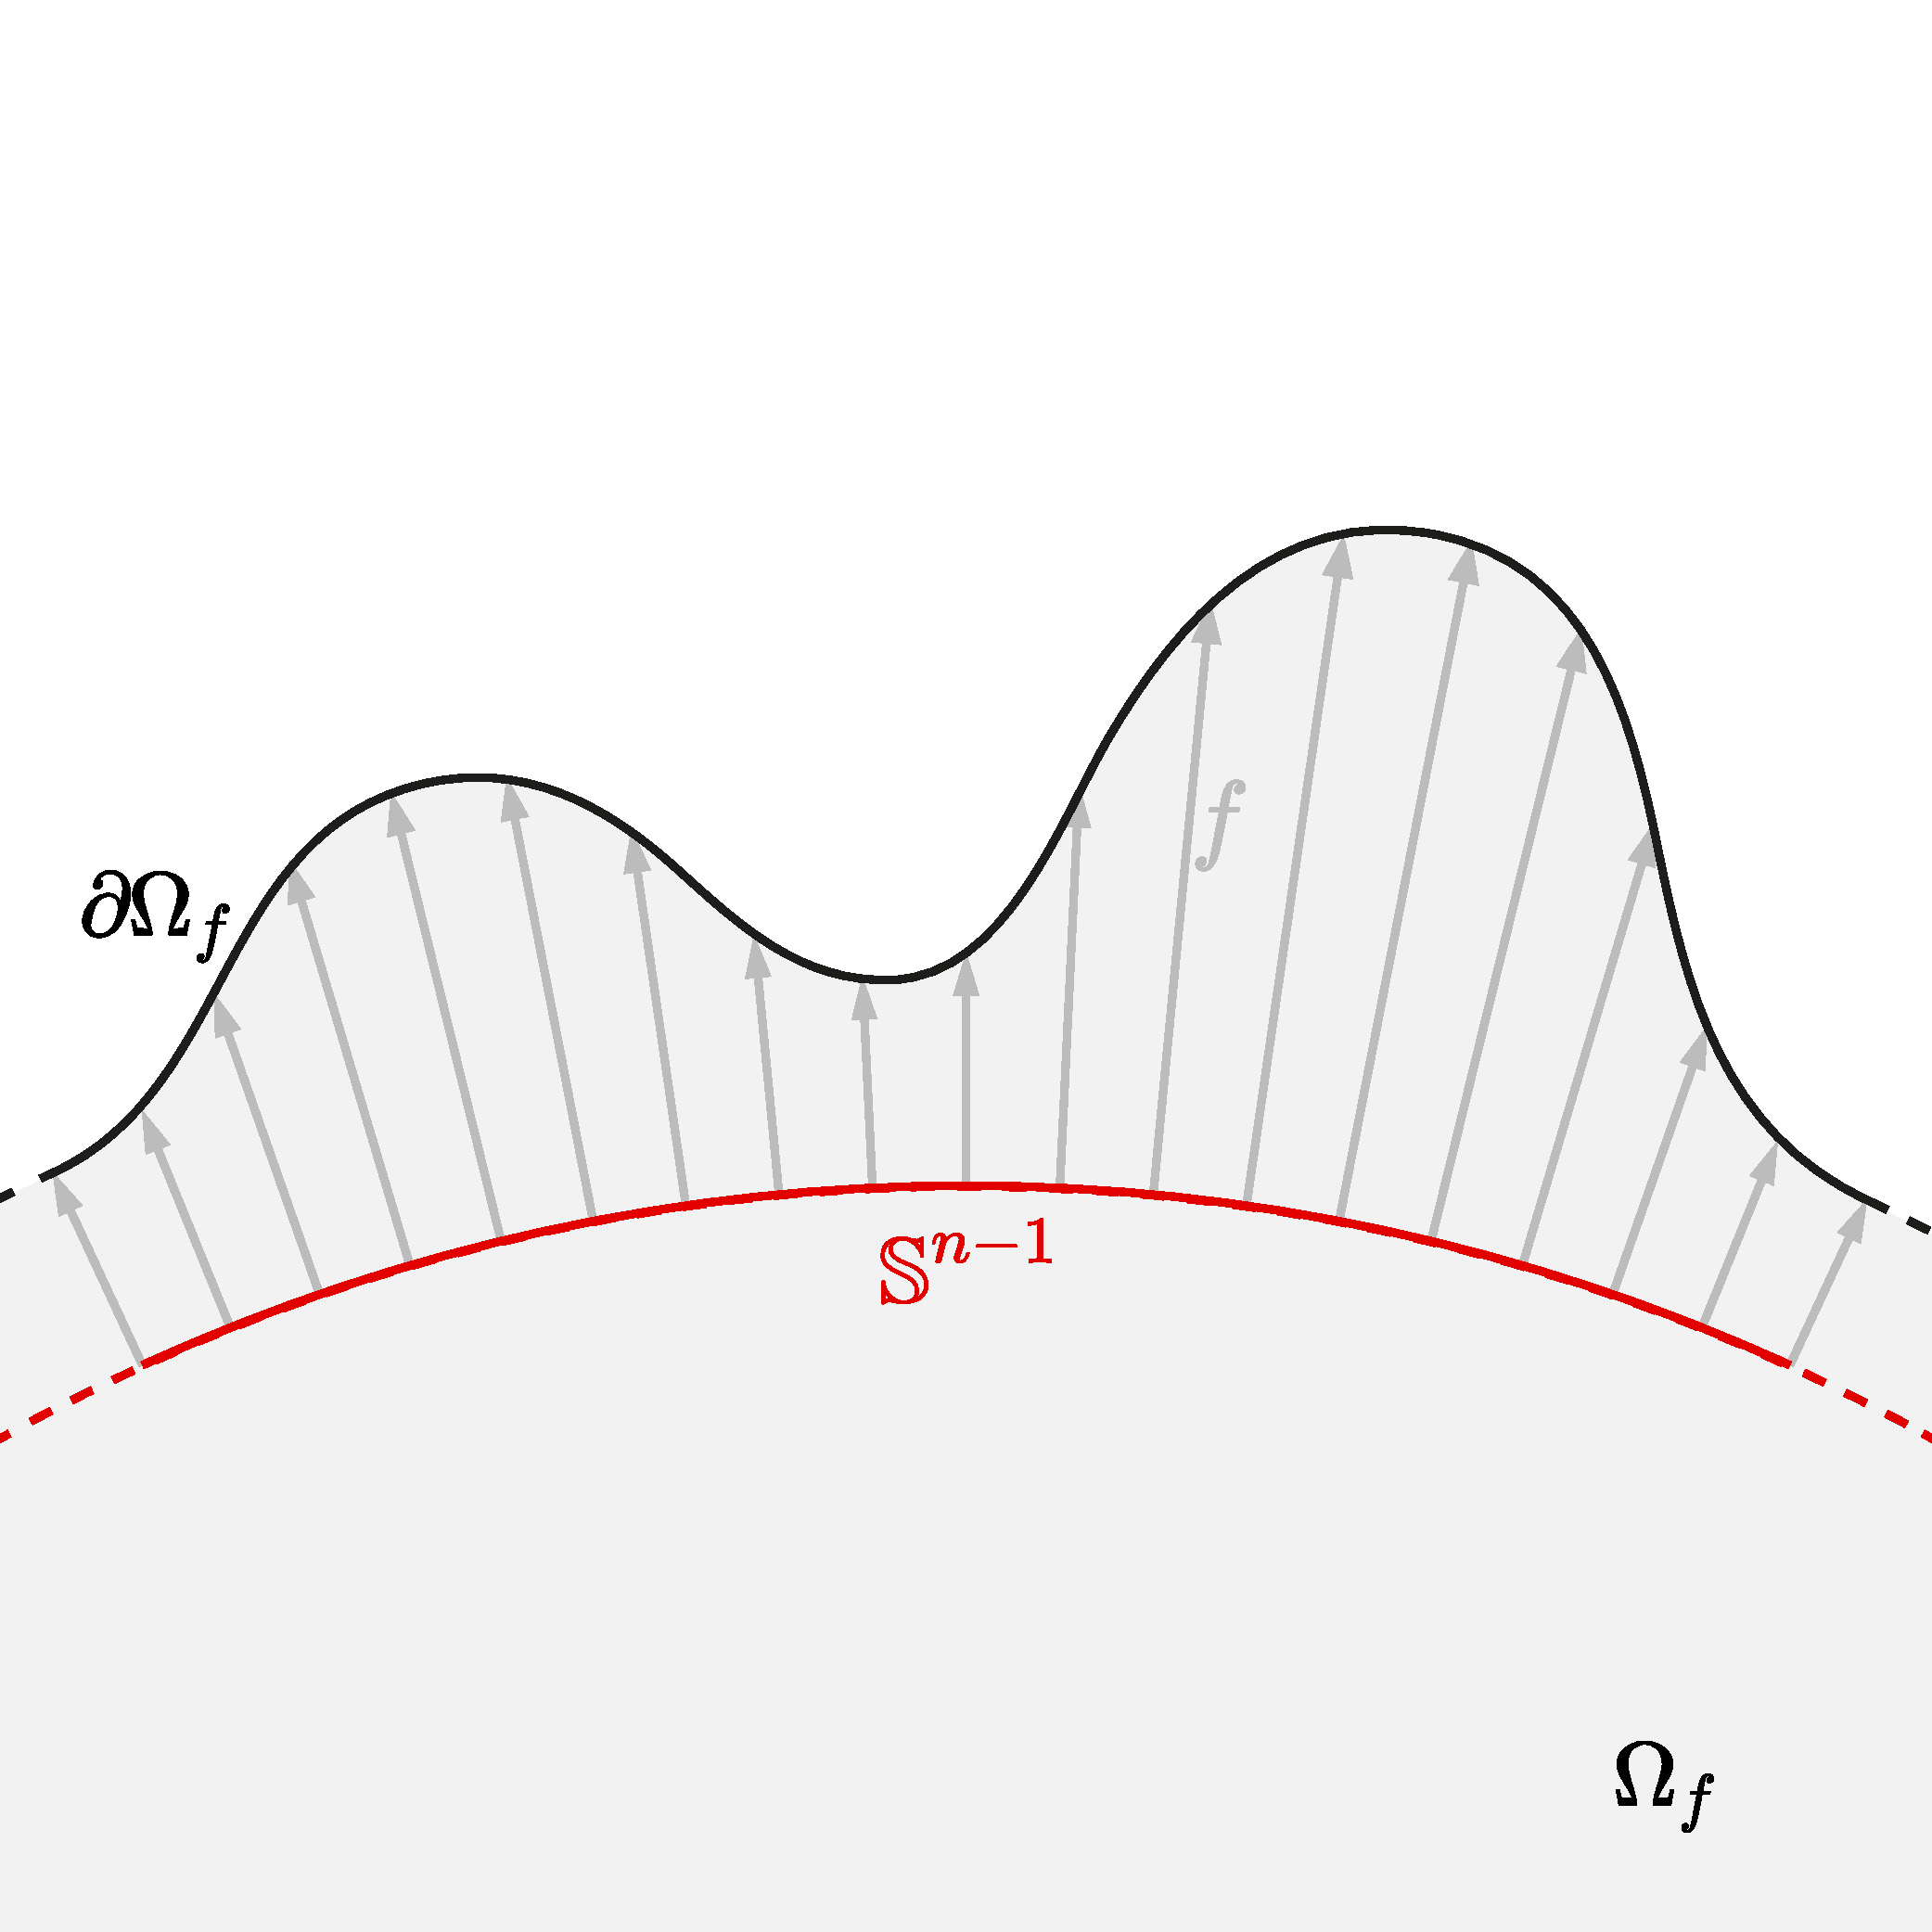
\includegraphics[width=0.4\columnwidth]{Images/RadialDisplacement.pdf}
%\caption{Illustration of radial displacement}\label{fig:star}
%\end{figure}

\begin{mproof}

For $x \in \partial \Omega_f$ (so, $x\neq 0$) we find $x_n, y_n \rightarrow x$ with $|x_n|<f(\widehat{x_n})$ and $|y_n|\geq f(\widehat{y_n})$. For large $n$ and by continuity, $|x| = f(\xh)$ and we have shown one inclusion.

For the reverse, and $x, |x|=f(\xh)$ (so, $x\neq 0$), we define $x_n = \frac{n}{n+1} x$ which satisfies $|x_n|<|x|=f(\xh)=f(\widehat{x_n})$, that is, $x_n \in \Omega_f$, and also $x_n\rightarrow x$. This shows that $x \in \partial \Omega_f$.

It is a bounded Lipschitz domain by lemma 2 at page 96 of \cite{burenkov}, and lemma 5 at page 151 also of \cite{burenkov}. Note that the definition of Lipschitz domain of \cite{burenkov} is completely equivalent to that of \cite{bello} (and at least implies that of \cite{mclean}, \cite{grisvard}, \cite{leoni}, \cite{adams}, a fact which is needed in the sequel), by an application of the Lebesgue number lemma, whose statement can be found at e.g. page 179 of \cite{munkres}.
\end{mproof}

We now define maps relating a radial function to its correspondent a star-shaped domain. We choose $0<\eps <f_D \in W^{1,\infty}(\mS)$, to parametrize the non moving part of the optimization domain. The reference domain $U_r$ is taken to be $U_r:=\Omega_{f_D}\setminus \overline{B}_\eps$, and we call $D:=\Omega_{f_D}$

\begin{prop}[$H_f, A_f$]
Let $\eps <f_D \in W^{1,\infty}(\mS)$ and $0<f \in W^{1,\infty}(\mS), f<f_D$, and define:
\begin{itemize}
	\item $H_f(x):=\ds \left\{\begin{matrix}
\frac{x}{\epsilon}f(\hat{x}) &  x\neq 0\\ 
0 & x=0
\end{matrix}\right. $, as a function $\mR^n\rightarrow \mR^n$
	\item $A_f(x):=\left (  f(\xh)+\frac{f_D(\xh)-f(\xh)}{f_D(\xh)-\eps}(|x|-\eps) \right )\xh$, as a function $\mR^n\setminus\{0\}\rightarrow \mR^n$
\end{itemize}

They enjoy the following properties:

\begin{enumerate}
%	\item $H_f:\mR^n \rightarrow \mR^n$, $A_f:\mR^n \rightarrow \mR^n$ is Lipschitz, $A_f: \overline{D}\setminus B_\eps\rightarrow \mR^n$ is Lipschitz too
	\item $H_f(B_\eps)=\Omega_f$, $H_f(\eps \mS) = \partial \Omega_f$
	\item $A_f(D\setminus \overline{B_\eps}) = D\setminus \overline{\Omega_f}$, $A_f(\partial D) = \id$, $A_f(\eps \mS) = \partial \Omega_f$
	\item $A_f=H_f$ on $\eps\mS$
	\item $H_f^{-1}(y):=\ds \left\{\begin{matrix}
\epsilon \frac{y}{f(\hat{y})} &  y\neq 0\\ 
0 & y=0
\end{matrix}\right. $, as a function $\mR^n\rightarrow \mR^n$
	\item $A_f^{-1}(y):=\left (  \eps+\frac{f_D(\yh)-\eps}{f_D(\yh)-f(\yh)}(|y|-f(\yh)) \right )\yh$, as a function $\overline{D}\setminus \Omega_f \rightarrow \overline{D}\setminus B_\eps$
\end{enumerate}

\end{prop}


\begin{figure}[H]
\centering
%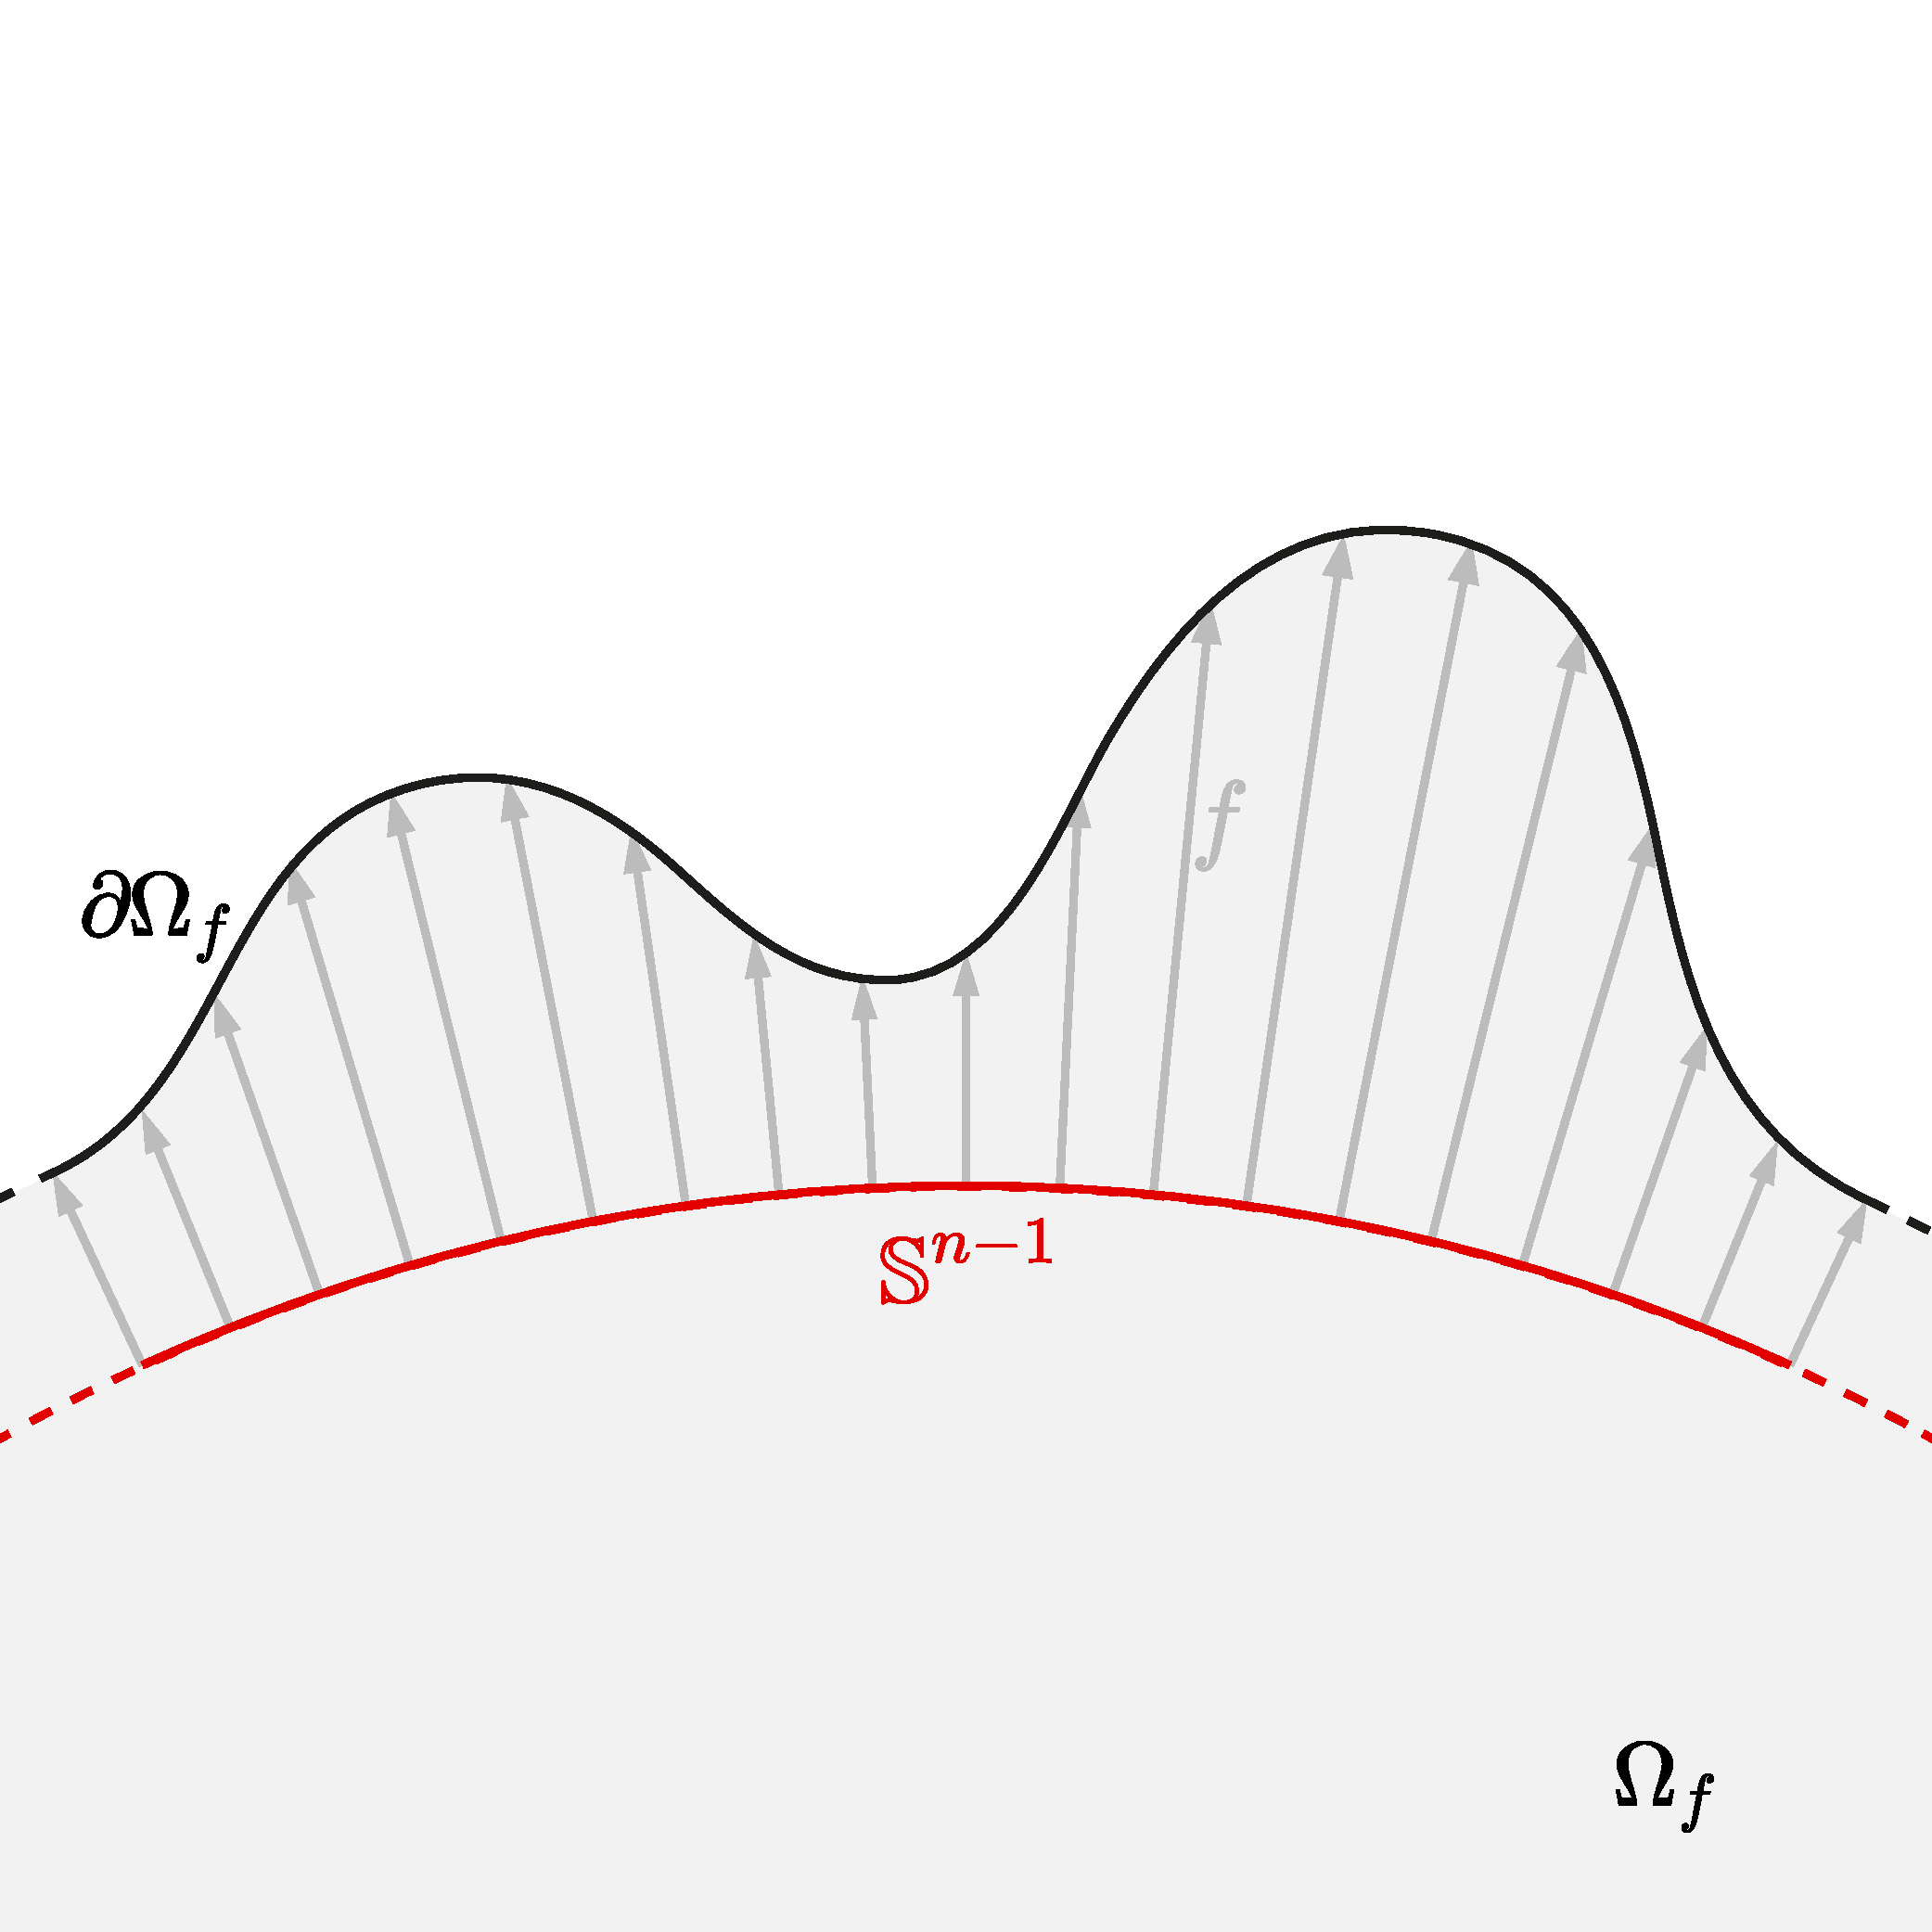
\includegraphics[width=0.3\columnwidth]{Images/RadialDisplacement.pdf}
%\caption{Illustration of radial displacement}\label{fig:star}
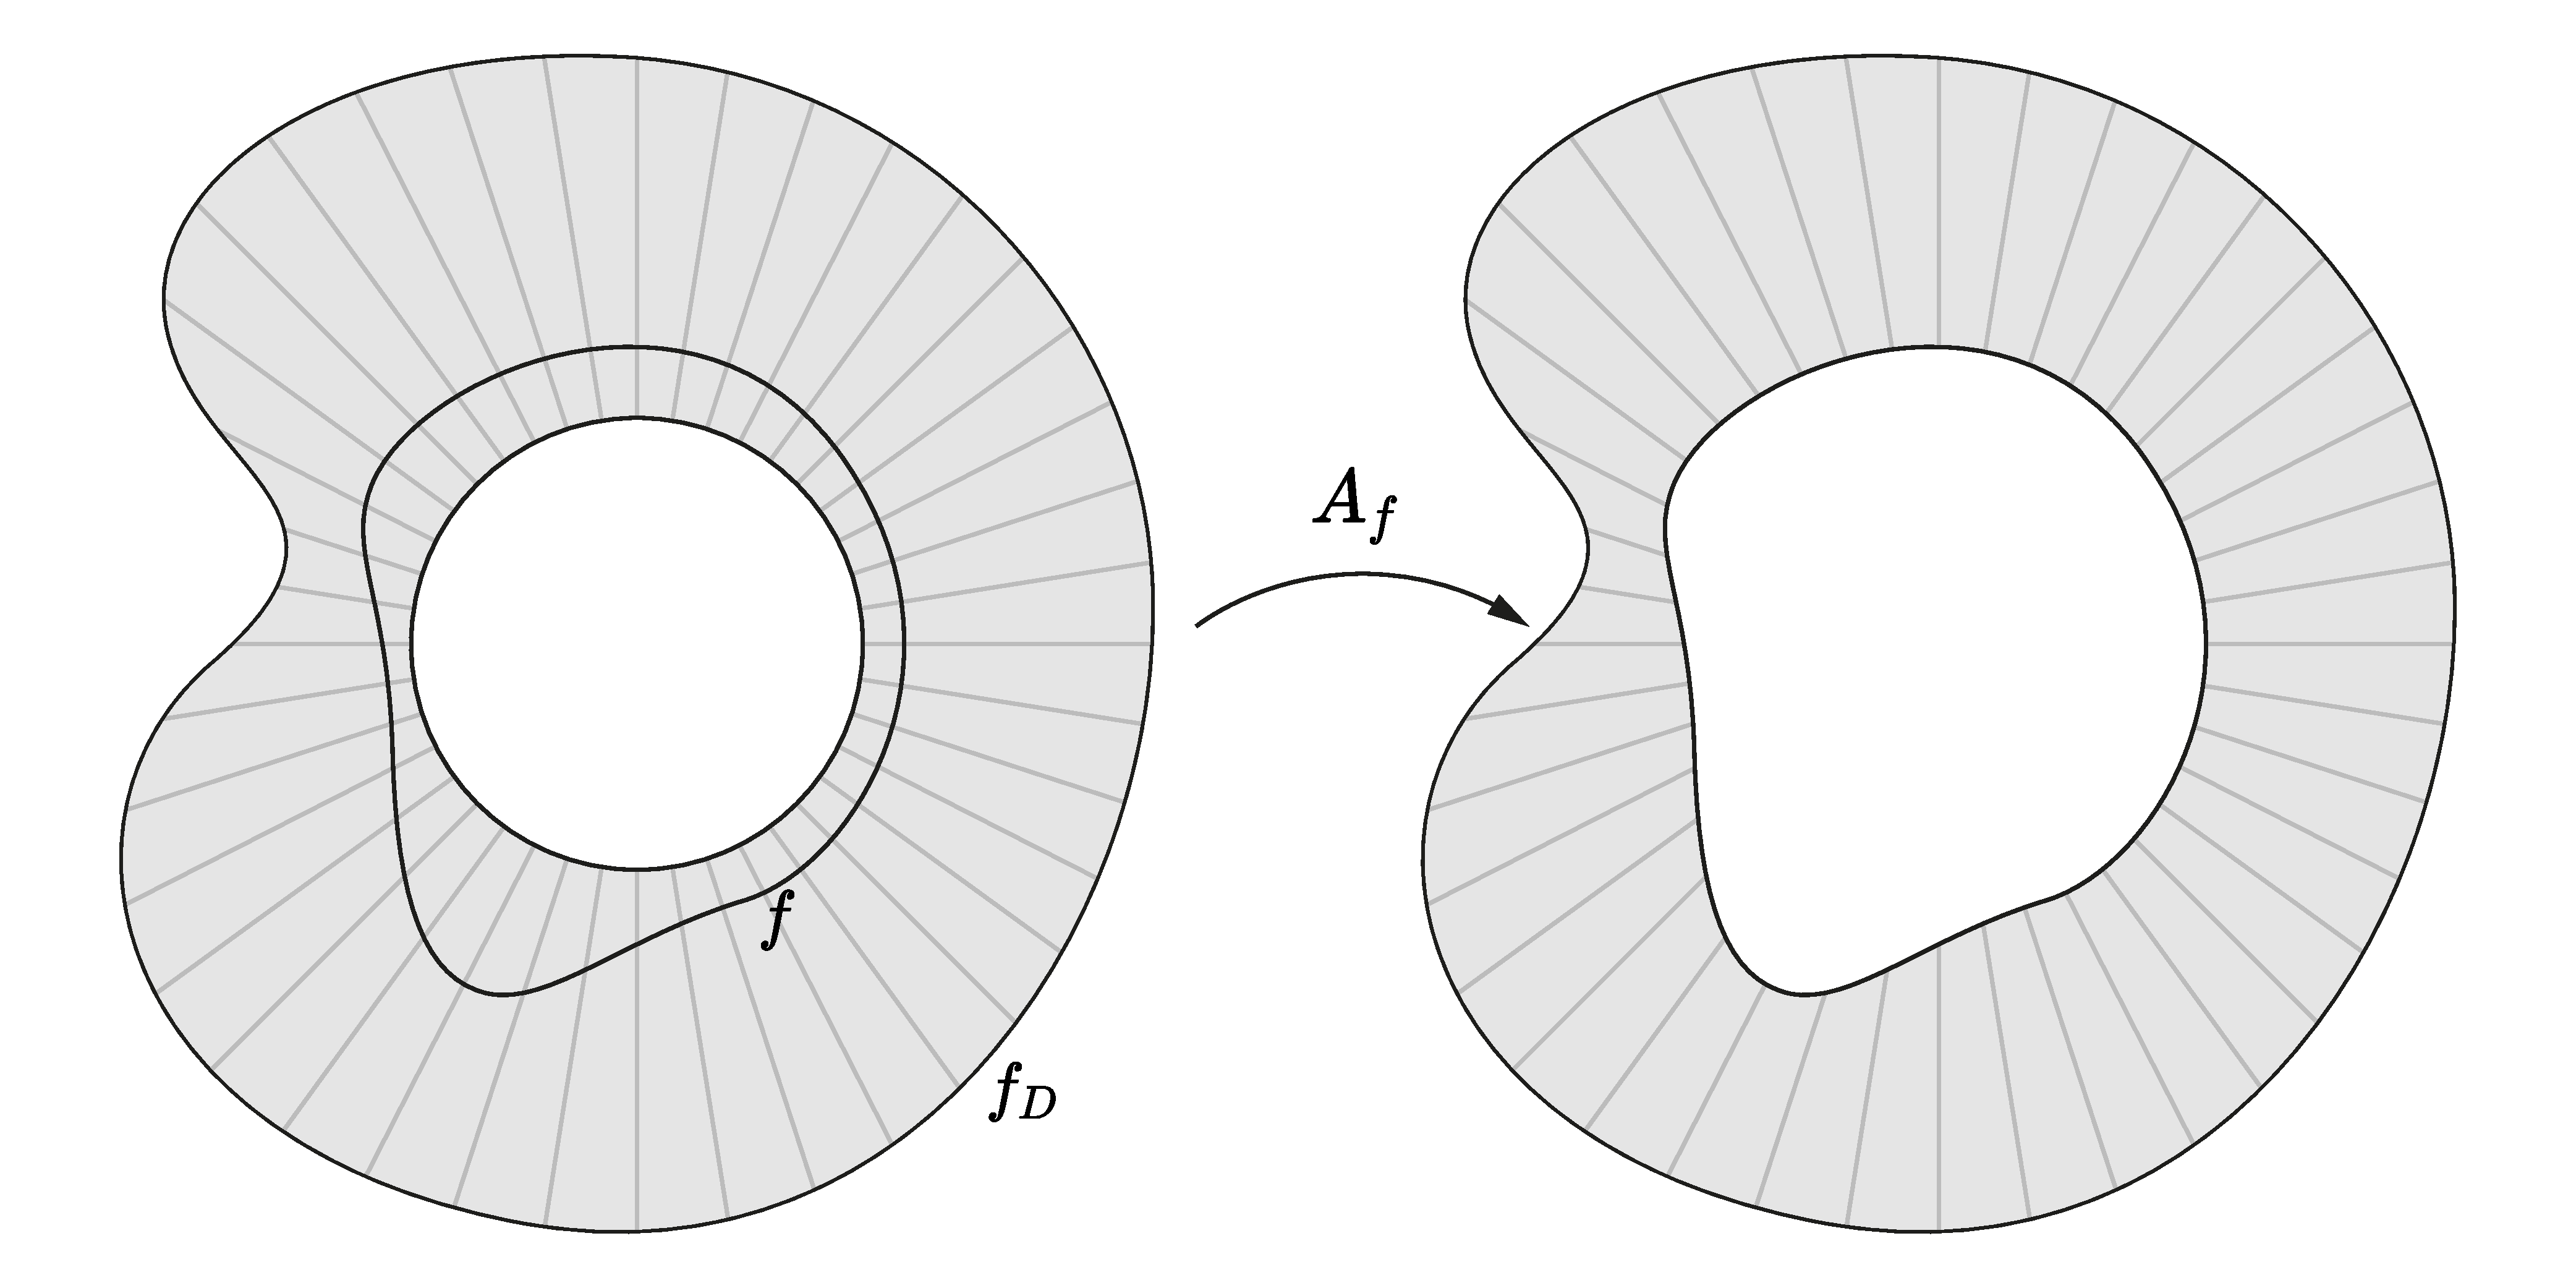
\includegraphics[width=0.7\columnwidth]{Images/A_f.pdf}
\caption{Illustration of the action of $A_f$}\label{fig:A_f}
\end{figure}

\begin{mproof}
All the properties are straightforward from the definitions. It helps to recognize that $A_f$ linearly maps the radial segment $[\eps, f_D(\xh)]$ to $[f(\xh), f_D(\xh)]$.
\end{mproof}

% and that $\overline{\Omega_{f_D}} \setminus \Omega_f = \{f(\xh)\leq|x|\leq f_D(\xh)\}$.

They also satisfy a bi-Lipschitz condition.

\begin{prop}[Bi-Lipschitz condition]
We have that $A_f:  \overline{D}\setminus B_\eps\rightarrow \overline{D}\setminus \Omega_f $ is Lipschitz with Lipschitz inverse (bi-Lipschitz), and so is $H_f: \mR^n \rightarrow \mR^n$.
\end{prop}

\begin{mproof}

%The second part of the proposition is contained in \cite{deckelnick} in a weaker form, we therefore proceed to prove all the statements.

\underline{$H_f$}

We can assume both $x,y\neq 0$. Then $|f(\xh)x-f(\yh)y|\leq |x||f(\xh)-f(\yh)|+f(\yh)|x-y|$. Employing direct and reverse triangle inequalities we get $|\xh-\yh|\leq \frac{2}{|x|}|x-y|$.
As $f$ is Lipschitz, we obtain:  $|f(\xh)x-f(\yh)y|\leq |x|C(f)\frac{2}{|x|}|x-y|+C(f)|x-y|$, see \cite{deckelnick} for more details.

Now, $1/f$ is also Lipschitz and bounded, because $f>0$ and is continuous on a compact set. Thus the same proof shows the Lipschitz property also for $H_f^{-1}$.

\underline{$A_f$}

Call $A_f(x)=\left (  f(\xh)+\frac{f_D(\xh)-f(\xh)}{f_D(\xh)-\eps}(|x|-\eps) \right )\xh =:Q(x)\xh $. Because $|x|\geq\eps$, as before, we obtain $|A_f(x)-A_f(y)|\leq 2/\eps Q(x) |x-y|+|Q(x)-Q(y)|$, so that we need to show that $Q$ is bounded Lipschitz.

By continuity and compactness, $f_D(\xh)-\eps\geq \delta >0$ and boundedness follows. The Lipschitz property follows because $Q$ is a sum of products of bounded Lipschitz functions.
%For instance, $f_D(\xh)$ is bounded and Lipschitz because $|x|\geq\eps$, as before, and so is $f_D(\xh)-\eps$. It is a bounded Lipschitz function that is uniformly greater than $\delta$, so that its reciprocal is also a bounded Lipschitz function.

Analogous reasonings let us prove also the Lipschitz property of $A_f^{-1}$.
\end{mproof}

We now try to glue $H_f, A_f$ together to still obtain a bi-Lipschitz function. Even the Lipschitz property doesn't hold after gluing, in general, see page 7 of \cite{weaver} for a counterexample. We therefore proceed to the proof of this fact, starting with a lemma.

\begin{lemma}[Gluing Lipschitz functions along $\eps \mS$]
\label{lemma:gluing_lip}
Let $\mR^n \supseteq A\supseteq\eps \mS$ be a set. Suppose that $g:A\rightarrow\mR^n$ and $h:\overline{B_\eps}\rightarrow\mR^n$ are Lipschitz and that they agree on $\eps \mS$. The, their gluing $f: A \cup \overline{B_\eps}\rightarrow\mR^n$ is Lipschitz.
\end{lemma}

\begin{mproof}
We can assume that $x \in B_\eps$, $y \in A \setminus \overline{B_\eps}$.
Then, $|f(x)-f(y)|\leq |h(x)-h(\eps \yh)|+|g(\eps \yh)-g(y)|$.

We claim at first that $|y-\eps \yh|\leq  |x-y|$. To see this, choose $n:=\yh$. Then $|y-x|^2 \geq |(y-x)\cdot n n|^2$ by Pythagoras' theorem, so that $|y-x|\geq |(y-x)\cdot n| = |(y-\eps \yh)\cdot n + (\eps \yh -x)\cdot n|$. But $(y-\eps \yh)\cdot n=|y|-\eps \geq 0$, and $(\eps \yh -x)\cdot n = \eps - x\cdot n\geq 0 $ as $x\cdot n \leq |x|\leq \eps$.

Thus  $|y-x|\geq |(y-\eps \yh)\cdot n| + |(\eps \yh -x)\cdot n|\geq  |(y-\eps \yh)\cdot n|=|y-\eps \yh|$.

We also claim that $|x-\eps \yh|\leq |x-y|$. To do so, pick $n:=\frac{\eps\yh -x}{|\eps\yh-x|}$. By Pythagoras' theorem we obtain $|y-x|\geq |(y-x)\cdot n|=|(y-\eps \yh)\cdot n +(\eps \yh -x)\cdot n|$. The second summand is non-negative and for the first one, it is directly proportional to $(y-\eps \yh)\cdot(\eps \yh-x)=(|y|-\eps)(\eps-\yh\cdot x)\geq 0$. So, $|x-y|\geq |(\eps \yh -x)\cdot n|=|\eps \yh -x|$.

Thus $ |f(x)-f(y)|\leq C|x-y|$ as desired.
\end{mproof}

\begin{prop}[Gluing $H_f^{-1}, A_f^{-1}$]
\label{prop:gluing}
$H_f^{-1}, A_f^{-1}$, or also $A_f, H_f$ can be glued into a Lipschitz function $\overline{D}\rightarrow\overline{D}$.
\end{prop}
\begin{mproof}

Call $\tau_f^{-1}$ the gluing. It is Lipschitz $\overline{D}\rightarrow\overline{D}$ if and only if $\tau_f^{-1}\circ H_f$ is Lipschitz $H_f^{-1}(\overline{D})\rightarrow\mR^n$, because we proved that $H_f$ is bi-Lipschitz $\mR^n \rightarrow \mR^n$.
We are therefore left to check that gluing Lipschitz functions along $\eps \mS$ produces a Lipschitz function, which would also yield the claim for $\tau_f$, that is the gluing of $A_f, H_f$. This is the content of \cref{lemma:gluing_lip}.
\end{mproof}

\begin{cor}[Radial to volumetric transformation]
\label{cor:star_shaped_transformation}
Let again $\eps <f_D \in W^{1,\infty}(\mS)$ and $0<f \in W^{1,\infty}(\mS), f<f_D$. Define:

\begin{itemize}
	\item $\ds \tau_f(x):=\left\{\begin{matrix}
 x & |x|\geq f_D(\xh)\\ 
 \left (  f(\xh)+\frac{f_D(\xh)-f(\xh)}{f_D(\xh)-\eps}(|x|-\eps) \right )\xh & \eps \leq |x| \leq f_D(\xh) \\ 
 \frac{x}{\epsilon}f(\hat{x}) & 0<|x|\leq \eps\\ 
 0 & |x|=0
\end{matrix}\right.$

	\item $\ds \tau_f^{-1}(y):=\left\{\begin{matrix}
 x & |y|\geq f_D(\yh)\\ 
 \left (  \eps+\frac{f_D(\yh)-\eps}{f_D(\yh)-f(\yh)}(|y|-f(\yh)) \right )\yh & f(\yh) \leq |y| \leq f_D(\yh) \\ 
 \epsilon \frac{y}{f(\hat{y})}& 0<|y|\leq f(\yh)\\ 
 0 & |y|=0
\end{matrix}\right.$
\end{itemize}


Then $\tau_f \in \cT$, i.e. it is a bi-Lipschitz homeomorphism.
\end{cor}
\begin{mproof}

The final gluing on the border of $D$ yields a Lipschitz function: we can see this by taking $\id -\tau_f^{\pm 1}$, which is Lipschitz and vanishing on $\partial D$, so that we are dealing with the zero extension outside $D$ of a Lipschitz function, null on $\partial D$. Such extension is readily shown to be Lipschitz.
\end{mproof}

\begin{obs}[Obtaining Lipschitz domains]
\mbox{} \\
Note that as long as $0<f<f_D$ are Lipschitz, $\tau_f(U_r)$ will always be a bounded Lipschitz domain. This is a more transparent way of securing this fact, than imposing $\norm{\tau-\id}_{W^{1,\infty}(\mR^n;\mR^n)}< C(U_r)$, as seen in \cref{def:adm_transf}.
\end{obs}

We finally have a look at shape derivatives in this radial framework. The reparametrized cost functional is $j(\sigma):=J(\tau_{\eps+\sigma})$, where $0<\sigma+\eps < f_D$. We are interested, for $h\in W^{1, \infty}(\mS)$, in the limit $$\lim_{t\rightarrow 0}\frac{j(\sigma+th)-j(\sigma)}{t}=\lim_{t\rightarrow 0}\frac{J(\tau_{\eps+\sigma+th})-J(\tau_{\sigma+\eps})}{t}$$

Now, we derive the expression of a displacement field $V_h$, to connect this difference quotient to the already computed shape derivative, see also \cite{deckelnick}. The ansatz $\tau_{\sigma+th}=(\id + tV_h\circ \tau_\sigma^{-1})\circ \tau_\sigma$ brings us to $V_h = \ds \frac{\tau_{\sigma+th}-\tau_\sigma}{t}$, and by some computations, we obtain: 

$$V_h(x) :=\left\{\begin{matrix}
 0 & |x|\geq f_D(\xh)\\ 
 h(\xh)\frac{f_D(\xh)-|x|}{f_D(\xh)-\eps}\xh & \eps \leq |x| \leq f_D(\xh) \\ 
 \frac{x}{\epsilon}h(\hat{x}) & 0<|x|\leq \eps\\ 
 0 & |x|=0
\end{matrix}\right.$$

This expression only depends on $h$ and is the gluing of Lipschitz functions, that are either $0$ at the gluing points, or such that the gluing points lie in $\eps\mS$. Note, this vector field is just moving $\eps \mS$ radially by $h$ and radially damping this movement to $0$ close to $\partial D$. Therefore:

\begin{prop}[Shape derivative, star shaped case]
\label{prop:star_shaped_gradient}
We have the following facts, for $h \in W^{1,\infty}(\mS)$, $0<\sigma<f_D$, $\sigma \in W^{1,\infty}(\mS)$:

\begin{itemize}
	\item $\tau_{\sigma+th}=(\id + tV_h\circ \tau_\sigma^{-1})\circ \tau_\sigma$
	\item $V_h \in \Te$
	\item $j$ is Gateaux differentiable at every $0<\sigma<f_D$, $\sigma \in W^{1,\infty}(\mS)$, with $j'(\sigma)[h] = J'(\tau_{\eps+\sigma})[V_h]$
\end{itemize}

\end{prop}
\begin{mproof}

We only need to show that $h\mapsto V_h$ is linear bounded between $W^{1,\infty}(\mS)\rightarrow \Te$. Linearity is immediate and for the boundedness: $\sup_x|V_h(x)| = \norm{h}_\infty$, so that there only remains to bound the Lipschitz constant of $V_h$. 

To do so, we note that extending to zero a Lipschitz function doesn't increase its Lipschitz constant, so that we only need to look at the restriction to $D$.

The gluing lemma \cref{lemma:gluing_lip} shows that it is sufficient to bound the Lipschitz constants of the two branches of $V_h$, separately.
These bounds are, respectively: $C(\norm{h}_\infty + 2\norm{D_T h}_\infty)$ and $[2\eps^{-1}(\norm{D_T h}_\infty + \norm{h}_\infty)]C+C\norm{h}_\infty$, where $C=(\eps, f_D)>0$, which concludes the proof.
\end{mproof}

\subsection{Smooth star-shaped domains}

To ensure that $U$ has the smoothness required to perform numerical analysis, we want to increase the regularity of $f$ and see an increase in the regularity of $\partial \Omega_f$.

\begin{prop}[Smooth radial function yields smooth star shaped domain]
\label{prop:Co_domain}
Let $f>0$ which is either $C^{1,1}(\mS)$ (that is, $C^1$ with all the components of $D_T f$ Lipschitz) or $C^2(\mS)$.  

Then, $\Omega_f$ has boundary of class $C^{1,1}$ or $C^2$.

\end{prop}

\begin{mproof}

In what follows we generically write $ C^o$, $o=1,1 $ or $o=2$. The argument goes like this:

\begin{itemize}
	\item we show that $H_f$ preserves smooth boundaries, where smoothness here is in the sense of charts (see e.g. \cite{murat}, pages II-39,40)
	\item using the implicit function theorem, we see that smoothness in the sense of charts implies smoothness in the sense of hypergraphs, see e.g. \cite{grisvard}, definition 1.2.1.1, which is the notion of smoothness we are working with  
\end{itemize}


\underline{Punctured diffeomorphisms}

We consider $H_f$, setting $\eps=1$ for simplicity. It has gradient (see \cite{deckelnick}) $D H_f(x) = f(\xh)I+\xh \otimes D_Tf(\xh)$, and  $D H_f^{-1}(y) =1/f(\yh)I-1/f(\yh)^2 \yh \otimes D_Tf(\yh)$. We conclude that $H_f: \overline{B_\delta(0)}^c \rightarrow \overline{H_f(B_\delta(0))}^c$ is a $C^o$ diffeomorphism, where the set on the right is open by $H_f$ being a homeomorphism of $\mR^n$, and $\delta < 1 = \eps$.
% The Lipschitz regularity of the gradients follows from the Lipschitz property and boundedness of every factor, and the fact that we are working away from the origin. In particular, $D_T f$ is Lipschitz, therefore continuous, on the sphere, and so bounded too.

We have therefore obtained a homeomorphism $H_f^{-1}:\mR^n \rightarrow \mR^n$, which is $C^o( \overline{H_f(B_\delta(0))}^c;\overline{B_\delta(0)}^c )$, i.e. whose domain is a neighbourhood of $\partial \Omega_f$.
For simplicity let's call such maps $C^o$ punctured diffeomorphisms for $\Omega_f$.

\underline{Punctured diffeomorphism preserves $C^o$ domains in the sense of charts}

Let $\Omega$ be of class $C^o$ (always locally) and bounded. Assume we have $F$, a punctured diffeomorphism for $\Omega$, so, $F:\mR^n\rightarrow \mR^n$ is a homeomorphism, and $F: U\rightarrow F(U)$ is $C^o$, $\partial \Omega \cc U$. Then, by analyzing the composition of $F$ with (small enough) charts of $\Omega$ we see that $F(\Omega)$ is another $C^o$ domain. 

\underline{From charts to hypergraphs}

Let a radial function $f>0$ be of class $C^o$. $H_f$ is a punctured diffeomorphism of class $C^o$, so that we have that $\partial \Omega_f$ is the image of $\eps\mS$, a domain of class $C^o$ in the sense of charts. So $\Omega_f $ is of class $C^o$ too, in the sense of charts.


So, let $x\in \partial \Omega$. We obtain $A\ni x, B$ open, and $\eta: A\rightarrow B$ a $C^o$ diffeomorphism, with $\eta^{-1}(B\cap \mR^n_+)=A\cap \Omega$, and $\eta(x)=0$.
%
%$\phi$ is a $C^1$ diffeomorphism, so $D\phi_n(x)\neq 0$, and we can assume $D\phi_n(x)$ to be proportional to $-e_n$ by a rotation of the axis.
%
%Thus $\partial_n\phi_n(z)<0$ in some $B(x)\subseteq A$. $B(x)$ is chosen small that $\phi$ is Lipschitz on $B(x)$.
%
%Apply the implicit function theorem to obtain $V',I$ open with $x \in V'\times I\subseteq B(x)$ and a function $\eta:V'\rightarrow I$ that is $C^o$ and Lipschtiz, with $\phi_n(z',z_n)=0 \iff z_n = \eta(z')$, for $z \in V'\times I$.
%
%$V'$ is open around $x'$, so let's restrict it to a square centered at $x'$. Relabel $\eta$ as the restriction to this new $V'$ and restrict $I$ to be the connected component of $G$ hosting $\eta(V')$, which is now an interval, as continuous image of a connected set. Because $x_n \in I$, and by continuity, $V'$ can be shrunk such that $\eta(V')\cc J \cc I$ for some open interval $J$. 
%
%All these shrinkings don't change the character of being the implicit function, i.e. $\eta$ still satisfies $\phi_n(z',z_n)=0 \iff z_n = \eta(z')$, for $z \in V'\times I$, and also,  $x \in V'\times I\subseteq B(x)$ and $\eta:V'\rightarrow I$ is still $C^o$ and Lipschitz.
%
%Now, the choice of $B(x)$ makes $z_n\mapsto \phi(z',z_n)$ strictly decreasing, for $(z',z_n) \in B(x)$.  So, for $z \in V'\times I$, we have $\phi_n(z', z_n) = \phi_n(z)>0=\phi_n(z',\eta(z')) \iff z_n<\eta(z')$ (by basic properties of strictly decreasing functions).
%
%But also, $\phi_n(z) >0 \iff \phi(z) \in B\cap \mR^n_+ \iff z \in \phi^{-1}(\mR^n_+\cap B)=A\cap \Omega$.
%
%Therefore, $z \in V'\times I, z_n<\eta_n(z) \iff z \in V'\times I, \phi_n(z) >0 \iff z \in A\cap \Omega \cap (V'\times I) = (V'\times I)\cap \Omega$.

Applying the implicit function theorem in a suitable way (e.g. through minor reworkings of the proofs at page 310, 311 of \cite{gilardi2}), we obtain:

\begin{itemize}
	\item a ``square" and an interval $V', I$ with $V'\times I \ni x$
	\item $\phi: V'\rightarrow I$, Lipschitz, of class $C^o$
	\item $\phi(V') \cc J \cc I$
	\item $z \in V'\times I, z_n<\phi(z) \iff z \in (V'\times I)\cap \Omega$
	\item (and consequently, $z \in V'\times I, z_n=\phi(z) \iff z \in (V'\times I)\cap \partial \Omega$)
\end{itemize}


%So, by the implicit function theorem, for $x \in \partial \Omega_f$ we can find a change of coordinates and a parallelepiped $V = V'\times I$ with $\phi: V'\rightarrow I$, $\phi$ of class $C^o$ and also Lipschitz, and $V\cap 	\Omega_f = V\cap \{x_n<\phi(x')\}$. We have moreover that $\phi \in J \cc I$ for some open interval $J$.

 By a compactness argument, finitely many $V_j = V_j'\times (a_n^j, b_n^j) $ are necessary to cover $\partial \Omega_f$. 

So, we have $V_j \cap \Omega_f = V_j\cap \{x_n<\phi_j(x')\} = V\cap \{a_n^j<x_n<\phi_j(x'), x' \in V_j'\}$. Choose $d>0$ to be the minimum gap between $\phi_j$ and $I_j$. $d>0$ by the existence of $J_j \cc I_j$. We call $L$ the maximum Lipschitz constant of $\phi_j$. 
We have therefore obtained a Lipschitz and $C^o$ domain in the style of \cite{burenkov}, which yields, modulo an application of the Lebesgue number lemma, a $C^o$ and Lipschitz domain in the style of \cite{grisvard}, whose definition we are working with.
\end{mproof}

\section{Descent directions}
\label{sec:hilbert}

To approximate a solution of \cref{pb:shopt} one must apply a discretization strategy and solve an optimization problem in finite dimensions. We will adopt gradient based optimization algorithms, where we compute search directions from the knowledge of the discretized shape derivative. In general, the shape derivative on the continuous level is just a functional: one can try to extract a descent direction from its knowledge using the Riesz representation theorem.
% The choice of the inner product in which to find the representative is usually dictated by the control space, in optimal control. 

%It is important at this stage to preserve the properties of the continuos problem when developing a discretization strategy. 

In shape optimization, however, one works with spaces which are not Hilbert, e.g. $W^{1,\infty}$, so scalar products are not available. A way around this is illustrated in \cite{deckelnick}, where descent directions are directly searched in $W^{1,\infty}$ without relying on the Riesz theorem. Another possibility is to look for descent directions in a larger, Hilbert space $\pazocal{H}\supset W^{1,\infty}$, provided that $j'$ extends to this space, where we can use the representation theorem. This ``Hilbert space" approach was of easier implementation for us, and we decided to stick with it.  Moreover, it is a standard trick in the shape optimization literature (see \cite{allaire}, section 5.2) and it can usually yield good results.

Nonetheless, this approach is not completely rigorous (because we want controls $\sigma$ in $W^{1,\infty}$, at least, and we perturb them by $\pazocal{H}$ descent directions), and also, it is not immediate which $\pazocal{H}$, hence, which scalar product, one should use. Unfortunately, choosing the ``wrong" one can yield descent directions that are too ``squiggly" (see \cref{sec:experiments} for an example, in particulare \cref{fig:l2}), or mesh-dependence effects, where finer and finer meshes require more and more optimization iterations to converge (see \cite{mesh_dependence}).

Through experimentations, see \cref{chap:num_exp} and specifically \cref{sec:implementation}, we observed decent results when using the $H^1$ scalar product, as opposed to when the $L^2$ product is used instead. On a continuous level, and in the star-shaped setting we described previously, this means finding descent directions $h \in H^1(\mS)$ from the equation:

$$(r(\sigma),h)_{H^1(\mS)}  = j'(\sigma)[h]$$

where $r(\sigma)$ represents, via the Riesz representation theorem, the functional $j'(\sigma)$. $h:=-r(\sigma)$ is e.g. a descent direction

% The reason for this is again to be able to find good enough (in the sense of smoothness) descent directions and to avoid mesh-dependence, as opposed to when the $L^2$ product is used instead. Despite not being a fully rigorous procedure, it is standard trick in shape optimization, and it worked well for us (see  \cref{chap:num_exp}). It is not rigorous because we pretend to simultaneously have $q$ smooth ($q \in H^2(\mS)$, for instance) while $r(q) \in H^1(\mS)$: $q-\alpha r(q)$ need not to be smooth too!

For further details regarding this so-called ``Hilbertian regularization" procedure, we again refer to \cite{allaire}.
We limit ourselves to sketching a proof of the fact that $j'(\sigma)$ can act on the larger space $H^1(\mS)$ and that it is continuous in the $H^1$ topology, thus making the operation of taking its Riesz representative well defined.

At first we remark that $h\mapsto V_h$ maps $H^1(\mS)$ functions into $H^1(\mR^n;\mR^n)$ functions. To see this, note that $h$ can be approximated by smooth functions $h_k$, in the $H^1$ norm (see definition 2.3 of \cite{aubin}). For the generic term of the approximating sequence we can employ integration in spherical coordinates and use the fact that $h_k$ is Cauchy, to get that $V_{h_k}$ is Cauchy in $H^1(\mR^n;\mR^n)$, and that it converges to $V_h$. This procedure also yields a bound on the norm of $h \mapsto V_h, H^1(\mS)\rightarrow H^1(\mR^n;\mR^n)$.

Now, consider the expression of the shape derivative, given in \cref{prop:gateaux_diff}. We identify three different terms. We write $u$ for a state $v$ or $w$, and $a$ for the corresponding adjoint, leaving out the dependence on $\tau$ for simplicity:

\begin{align*}
\int_I (u_t , \dive(\delta \te \circ \tau_\sigma^{-1}) a)_{L^2(U)}, \quad \int_I (A'(\delta\te\circ \tau_\sigma^{-1} )\nabla u, \nabla a)_{L^2(U)}, \quad \frac{1}{2}\int_I\int_{U} |v-w|^2\dive(\delta \te\circ \tau_\sigma^{-1})
\end{align*}

Here, $U = \tau_\sigma(U_r)$, $\delta \te = V_h$.

By the $H^1$ properties we have just shown and thanks to \cref{thm:change}, we observe that $\dive(\delta \te\circ \tau_\sigma^{-1})$, $A'(\delta\te\circ \tau_\sigma^{-1} )$ are square integrable. Moreover, as we will discuss very soon, we can make hypothesis on the data and a suitable modification to the cost function such that $u, a \in H^1(I, H^2(U))$, see \cref{ass:num_discr_shopt}, where we need the regularity of $\sigma$, to have $\partial U$ smooth enough to guarantee $H^2$ regularity (we have discussed this in \cref{prop:Co_domain}). Now, the Sobolev embedding $H^1\emb L^4$ (for spatial dimensions $n=2,3$, see e.g. \cite{adams}) and the Hölder's inequality, allow us to deduce that $j(\sigma)$ can be indeed continuously extended to $H^1(\mS)$. 

The same conclusions follow (more easily) when the star-shaped parametrization is not employed.


\chapter{Discretization}
\label{chap:discretization}
In this chapter we describe the numerical approximation of the PDEs of \cref{pb:pdes} and analyze the errors arising from this. While linear finite elements are used in space, the implicit Euler or the Crank-Nicolson methods are adopted for advancing in time.

We take into account the fact non-discretized domains are smooth, while the computational ones are polygonal/polyhedral. 

We are not focusing here on optimization algorithms to solve the shape identification problem, nor on the specific boundary parametrization. This will be done in \cref{chap:num_exp}.


As a summary of the discretization approach:

\begin{itemize}
	\item the PDEs are numerically solved on a polygonal/polyhedral approximation of the smooth domain $U$
	\item such approximation involves only knowing a finite number of points of $\partial U$, and not its entire parametrization
	\item the boundary data is queried only on these boundary nodes (this is compatible, for instance, with the case in which only a finite number of measurements are available)
	\item implicit Euler or Crank-Nicolson time steppings are adopted
%	\item several optimal order error estimates are obtained
\end{itemize}

We chose the latter methods because of their simplicity, overall low regularity requirements (compared to e.g. more sofisticated Runge-Kutta methods), and the fact that they are unconditionally stable, so that no restriction on the time step size must be made, relative to the mesh width, to obtain convergence. 
We can reach the required smoothness in time for the state equations, by requiring smooth data, and certain compatibility relations between them (see e.g. chapter 2 of \cite{lions} and \cref{ass:time_reg_mix}). Smoothness of the data alone is not enough: a regular solution can be obtained, but only away from the starting time, where a singularity can develop (see e.g. the discussion in \cite{harbrecht}). For the state equations we can reach any compatibility order, provided that we make suitable assumptions on the boundary data, but the adjoint equations are, in a certain sense, fixed by the particular cost functional we chose, and the state equations themselves: unfortunately, for our adjoints, we cannot tweak the problem data to obtain an arbitrary level of compatibility.

In \cite{harbrecht}, the authors work in fact with adjoint equations that have ``fully" incompatible boundary data and terminal condition, and devise a non-standard time stepping scheme to deal with this. On the other hand, our choice of cost functional makes it possible to obtain compatibility of ``order zero". This would be enough for a low order space-time method without time quadrature (see e.g. \cite{vexler}), but not for the chosen fully discrete schemes or for second order methods. To obtain more compatibility we need to modify what enters the adjoint equations, and since we cannot modify the structure of the PDEs solved by the states $w,v$, we can only modify the cost functional. This is what we will do, with the introduction of a suitable temporal weight in the cost functional of \cref{pb:shopt}. Such operation will yield compatibility of arbitrary order for the adjoints, at the price of partially modifying the nature of the shape optimization problem. See \cref{sec:o-t-d} for a more thorough discussion.

An in-depth presentation and analysis of the discretization algorithms for states and adjoints is discussed in \cref{chap:inh_fem}. In what follows we will build on the results therein.

As a last note, let us mention the two canonical ways, in the literature on optimal control, of discretizing a problem posed on an infinite-dimensional level:

\begin{itemize}
	\item optimize-then-discretize: the gradient of the cost functional is derived on the continuous level (see e.g. \cref{prop:gateaux_diff} in our case), some adjoint states appear and first order optimality conditions can be formulated. Then, one proceeds with discretizing states and adjoints and the continuous optimality system, and obtains one on the discrete level
	\item discretize-then-optimize: the states and cost function, i.e. the continuous problem (\cref{pb:pdes} and \cref{pb:shopt}), are discretized, so as to obtain an optimization problem posed on the discrete level. Finite dimensional optimality conditions can now be derived
\end{itemize}

In any case, one starts from an infinite-dimensional problem and obtains discrete optimality conditions, that can be employed in a numerical implementation. When the obtained discrete optimality systems from the two strategies coincide, we say that optimization and discretization commute. That is, the following diagram is commutative:

\[\begin{tikzcd}
	&&& \text{continuous optimality system} \\
	\begin{matrix}
\text{continuous} \\ \text{problem}
\end{matrix} &&&&&& \begin{matrix}
\text{discrete} \\ \text{optimality} \\ \text{system}
\end{matrix}  \\
	&&& \text{discrete problem} 
	\arrow["{\text{optimization}}"', from=3-4, to=2-7]
	\arrow["{\text{discretization}}", from=1-4, to=2-7]
	\arrow["{\text{optimization}}", from=2-1, to=1-4]
	\arrow["{\text{discretization}}"', from=2-1, to=3-4]
\end{tikzcd}\]

Although in general not a trivial task, realizing a commutative scheme may come with several benefits, we refer to the introduction of \cite{liu} for a comparison between the two strategies, and a discussion of advantages and disadvantages of each. See also \cite{flaig}, in the context of parabolic optimal control.

We can show that optimization and discretization commute, when using the implicit Euler case for the states, and a suitable variant for the adjoints. We strongly suspect that commutation holds also when Crank-Nicolson is used, see the work of \cite{flaig}.

Now:

\begin{itemize}
	\item in \cref{sec:o-t-d}, the continuous states and adjoints are discretized and the error in doing so, is quantified: we make heavy use here of the results from \cref{chap:inh_fem}. In particular, optimal order estimates for the FEM solutions are recalled (optimal with respect to the approximation properties of the finite element spaces and time stepping schemes)
	\item in \cref{sec:d-t-o_IE}, results about the convergence of the discrete shape gradient, to the continuous one, are presented in different settings: a spatially semidiscrete one, and two fully discrete ones, i.e. one with implicit Euler applied to the states and an overall discretize-then-optimize (and commutative) approach, the other with the Crank-Nicolson method applied to states and adjoints, in an optimize-then-discretize fashion
\end{itemize}

In what follows, $\lesssim$ stands for $\leq C$, with $C>0$ independent of time and space discretization parameters $\delta t$ and $h$, but possibly dependent on the current domain $U$.

\section{Approximation of PDEs}
\label{sec:o-t-d}

Consider the state and adjoint equations as seen in \cref{pb:pdes} and \cref{prop:gateaux_diff}. Let us have for simplicity a unified notation (just like in \cref{pb:mix}).

\begin{pb}[Unified notation for state and adjoint equations]
\label{pb:uni_state_adj}

\[
\begin{matrix}
\left\{\begin{matrix}
u_t-\Delta u =0 & \text{ in } U\times (0,T)\\ 
u = g_D & \text{ on } \Gamma_D\times(0,T)=:\Sigma_D\\ 
\partial_\nu u = g_N & \text{ on } \Gamma_N\times(0,T)=:\Sigma_N\\ 
u(0) =0 & 
\end{matrix}\right.

&,

\left\{\begin{matrix}
-a_t-\Delta a =(-1)^{\left [a=v\right ]}\eta (v-w) & \text{ in } U\times (0,T)\\ 
a = 0 & \text{ on } \Sigma_D\\ 
\partial_\nu a = 0 & \text{ on } \Sigma_N\\ 
a(T) =0 & 
\end{matrix}\right.
\end{matrix}
\]

We mean that $u$ stands either for $v$, in which case $a$ is $p$, or $u$ is $w$ and then $a$ is $q$. The notation $[a=v]$ means the Iverson bracket of the proposition ``$a=v$". In particular, the following correspondences hold:

\centering
\begin{tabular}{|l|c|c|c|c|} 
\hline
Variable           & $u=v$                                                                                      & $u=w$                          & $a = p$                          & $a=q$                           \\ 
\hline
Dirichlet boundary & $\Gamma_D = \partial U$                                                                    & $\Gamma_D=\Gamma_m$            & $\Gamma_D = \partial U$          & $\Gamma_D = \Gamma_m$           \\ 
\hline
Neumann boundary   & $\Gamma_N = \emptyset$                                                                     & $\Gamma_N = \Gamma_f$          & $\Gamma_N = \emptyset$           & $\Gamma_N = \Gamma_f$           \\
\hline
Dirichlet data     & $g_D=\left\{\begin{matrix}f&\text{ on }\Gamma_f\\0&\text{ on }\Gamma_m\end{matrix}\right.$ & $g_D = 0 \text{ on } \Gamma_m$ & $g_D = 0 \text{ on } \partial U$ & $g_D = 0 \text{ on } \Gamma_m$  \\ 
\hline
Neumann data       & -                              & $g_N = g \text{ on } \Gamma_f$ & -                                & $g_N = 0 \text{ on } \Gamma_f$ \\
\hline
\end{tabular}

% Note that we added a temporal weighting function $\eta$ which we will later specify.
% In particular, Dirichlet and Neumann boundaries are coherent between state and adjoint equation.

\end{pb}

We have dropped, for simplicity, all the references to the domain transformation $\tau$. Let us discuss the appearance of the temporal weight $\eta$. This is a function $\eta: [0,T] \rightarrow \mR$.
Its presence in the right hand side of the adjoint equations can be justified by modifying the energy function in \cref{pb:shopt} to be:

$$J_\eta(\tau) = \frac{1}{2} \int_I \eta \norm{v^\tau - w^\tau}_{H_\tau}^2$$

The proof of \cref{prop:gateaux_diff} works almost unchanged to derive the PDEs for the adjoints of \cref{pb:uni_state_adj}, and the shape gradient, where we only have to make the change:

\begin{align*}
\frac{1}{2}\int_I\int_{\tau(U_r)}|v^\tau-w^\tau|^2\dive(\delta \te\circ  \tau^{-1}) \rightarrow \frac{1}{2}\int_I\int_{\tau(U_r)}\eta|v^\tau-w^\tau|^2\dive(\delta \te\circ  \tau^{-1})
\end{align*} 



The main purpose of this modification is to facilitate the analysis of the numerical discretization. In particular, we choose $\eta$ to be a smooth cut-off function that is positive in $(0,T)$ and $0$ in $[T, +\infty]$. Note that in case a solution to the ``classical" problem exists, then it is also a solution to this new  perturbed problem, and viceversa. In fact, $J_\eta(\tau)=0 \implies \eta \norm{v_\tau - w_\tau}_{H_\tau}^2=0 \implies v_\tau = w_\tau$. This equality holds on all $I=[0,T]$ by the time continuity of the states.

Modifying the final-time behaviour of the energy might of course have detrimental effects if the boundary data exhibits strong variations close to final time. However, for boundary conditions that e.g. stabilyze over time, then a heat equation will also produce a solution tending to a steady state, so that the presence of $\eta$ shouldn't play a significant role. In any case, the shape of $\eta$ can be adjusted according to the user's needs.
%, but this is physically implausible if the boundary conditions don't exhibi, given the nature of the partial differential equation. In fact, it is known that solutions to the heat equation tend to a steady state in long times (for constant boundary conditions and no source), and we are only measuring the value of one such solution on the external boundary $\partial U$: we thus expect that in practice, this boundary data will not exhibit oscillatory behaviour for large times, and that the introduction of $\eta$ will not cause issues.

We now proceed to discretize states and adjoints using the scheme presented in \cref{pb:num_scheme} (the adjoint equation can be cast into a standard heat equation by time reversal).

% In short, finite elements are used in space, a finite difference time stepping, in time. Note that the adjoints discretization we are about to discuss is an optimize-then-discretize one. We will see alternative approaches in the case of implicit Euler.

% If one opted for an optimize-then-discretize approach this would be satisfactory (at least with regards to the numerical approximation of states and adjoints). However we will conduct experiments in a discretize-then-optimize setting, so that the upcoming results are only partially satisfactory, and we will not delve very deep into their consequences. 

The spatial discretization is carried out on a polygonal approximation $U_h$ of $U$, a smooth domain. We explicitly account for this discrepancy, see the introductory discussion in \cref{chap:inh_fem}.  We use a similar nomenclature for $U$ and $U_h$, for instance, we write $\Gamma_{m,h}\simeq \Gamma_m, \Gamma_{f,h}\simeq \Gamma_f, \Gamma_{D,h}\simeq \Gamma_D$ and $\Gamma_{N,h}\simeq \Gamma_N$. We can also define $\Sigma_{D,h}:= I \times \Gamma_{D,h}$ and so on.

%Note, the next assumption is formulated as if $U$, $U_h$ were fixed, i.e. as if they were not suibject to deformation. This will be remarked later on, too. 

Throughout, set $\theta=1$ to obtain the implicit Euler method, $\theta=1/2$ for the Crank-Nicolson method.

\begin{ass}[Hypothesis for the numerical discretization of \cref{pb:uni_state_adj} ]
\label{ass:num_discr_shopt}
\textcolor{white}{ }
\begin{enumerate}
	\item $\partial U \in C^2$ (for instance, the star shaped functions are $C^2$, see \cref{prop:Co_domain}), $U_h$ is polygonal/polyhedral and $\partial U_h$ interpolates $\partial U$. The mesh family of $U_h$ is (shape) regular and quasi-uniform (for such definitions, see \cite{brenner_scott})
	\item $g_D \in  H^{1/\theta+1}(I,H^{3/2}(\Gamma_D)) \cap H^1(I, H^{2}(\Gamma_D))$, $g_N \in  H^{1/\theta+1}(I, H^{3/2}(\Gamma_N)) \cap L^2(I, H^{2}(\Gamma_N))$
	\item $g_D(0)=0$ and $g_N^{(k)}(0), g_D^{(k+1)}(0)  = 0$ for $k=0,..., 1/\theta-1$
	\item $\eta^{(k)}(T)  = 0$ for $k=0,..., 1/\theta-1$, $\eta \geq 0$ and $\eta \in C^{\infty}([0,T];\mR)$
\end{enumerate}

\end{ass}

%We have written $g_N, g_D, \Gamma_D, \Gamma_N$ to mantain a flexible notation. With reference to \cref{pb:pdes} this translates to:
%
%\begin{itemize}
%	\item state $v$: $g_D=f$ on $\Gamma_f$, $g_D=0$ on $\Gamma_m$, $\Gamma_D = \partial U=\partial \tau(U_r)$, $\Gamma_N=\emptyset$
%	\item state $w$: $g_N=g$ on $\Gamma_f$, $g_D = 0$ on $\Gamma_m$, $\Gamma_D = \Gamma_m$ and $\Gamma_f = \Gamma_N$
%\end{itemize}

%\begin{table}[h]
%\centering
%\begin{tabular}{lcccc}
%Variable           & $u=v$                          & $u=w$                          & $a = p$                          & $a=q$                           \\
%Dirichlet boundary & $\Gamma_D = \partial U$        & $\Gamma_D=\Gamma_m$            & $\Gamma_D = \partial U$          & $\Gamma_D = \Gamma_m$           \\
%Dirichlet data     & $\left\{\begin{matrix}f&\text{ on }\Gamma_f\\0&\text{ on }\Gamma_m\end{matrix}\right.$ & $g_D = 0 \text{ on } \partial U$ & $g_D = 0 \text{ on } \Gamma_m$  \\
%Neumann boundary   & $\Gamma_N = \emptyset$         & $\Gamma_N = \Gamma_f$          & $\Gamma_N = \emptyset$           & $\Gamma_N = \Gamma_f$           \\
%Neumann data       & -                              & $g_N = g \text{ on } \Gamma_f$ & -                                & $g_N = 0 \text{ on } \Gamma_f$ 
%\end{tabular}
%\end{table}


Call now $h$ the maximum element size of $U_h$, and $\delta t$ the size of one of the $K$ uniform length intervals $[t^k,t^{k+1}]$, $k=0,...,K-1$, into which we subdivide $I$.
We indicate with $S^1_h$ the space of linear finite element on $U_h$, and  $S^1_{0,D,h}=\{ v_h \in S^1_h, {v_h}|_{\Gamma_{D,h}}=0\}$.

Here are the fully discrete problems we must solve if we apply the same schemes for adjoint and states, thus in an optimize-then-discretize fashion.

\begin{pb}[Numerical solution of \cref{pb:uni_state_adj} in optimize-then-discretize fashion]
\label{pb:num_scheme_recall}
Consider $g_{N,h}^k, g_{D,h}^k$ to be the Lagrange interpolant of $g_N(t^k), g_{D}(t^k)$. We adopt a similar notation as in \cref{pb:uni_state_adj}. So, we look for $u_h^k \in S^1_h$, $k=0,...,K$, with:

\begin{align*}
\left ( \frac{u_{h}^{k+1}-u_h^k}{\delta t}, \phi_h\right)_{L^2(U_h)} + (\nabla(\theta u_h^{k+1}+(1-\theta)u^k_h), \nabla \phi_h)_{L^2(U_h)} =\\ (\theta g_{N,h}^{k+1} + (1 - \theta)g_{N,h}^{k} , \phi_h)_{L^2(\Gamma_{N,h})},\quad  1\leq k \leq K\\
u_h^{k+1}|_{\Gamma_{D,h}}=g_{D,h}^{k+1},\quad 1\leq k \leq K\\
u_h^0=0
\end{align*}

and $\phi_h \in S^1_{0,D,h}$.
The same scheme is applied to the adjoint equations, i.e. we look for $a_h^k \in S^1_{0,D,h}$, $k=0,...,K$, with:


\begin{align*}
\left ( \frac{a_{h}^{k-1}-a_h^{k}}{\delta t}, \phi_h\right)_{L^2(U_h)} + (\nabla((1-\theta) a_h^{k}+\theta a^{k-1}_h), \nabla \phi_h)_{L^2(U_h)} =\\ (-1)^{\left[ u=v\right ]}((1-\theta) \eta(t^{k})(v_h^{k}-w_h^{k}) + \te \eta(t^{k-1})(v_h^{k-1}-w_h^{k-1}) , \phi_h)_{L^2(\Gamma_{N,h})},\quad  1\leq k \leq K\\
a_h^K=0
\end{align*}

and $\phi_h \in S^1_{0,D,h}$. Further details can be found in the appendix after \cref{pb:num_scheme}, of which \cref{pb:num_scheme_recall} is an instance.
\end{pb}


%\tred{put U vs $U_h$ here}
Let us also briefly introduce the spatially semidiscretized shape optimization problem, and its shape gradient. This is an interesting quantity on its own, but it will also play a role in obtaining fully discrete estimates. 

In the rest of the chapter, for simplicity but also for the sake of generality, we work again with general transformations, in place of radial fields. 
In particular, we write $U_h = \tau_h(U_{r,h})$ for $U_{r,h}$ interpolating $U_r$, and for $\tau_h$ a transformation that is a finite element vector field that fixes the external boundary $\Gamma_{f,h}$. $\tau_h$ thus preserves the finite element spaces and the polygonal/polyhedral nature of the discrete reference domain $U_{r,h}$.

%When using a unified notation as in \cref{pb:uni_state_adj}, we will mean $\Gamma_{D,h} = \Gamma_{m,h}, \Gamma_{N,h} = \Gamma_{f,h}$ for the state $w$, $\Gamma_{D,h} = \partial U_h, \Gamma_{N,h}=\emptyset$ for the state $v$. Moreover, $\Sigma_{D,h} = I \times \Gamma_{D,h}$, $\Sigma_{N,h} = I \times \Gamma_{N,h}$.
\begin{prop}[Semidiscrete shape optimization problem]
\label{prop:sd_shopt}
We introduce the spatially semidiscrete state equation, with unified notation $u_h$, similarly to \cref{pb:num_scheme_recall}. Calling $g_{N,h}$ and $g_{D,h}$ the Lagrange interpolants (defined a.e. in time) of $g_N, g_D$, we look for $u_h:I \rightarrow S^1_h$ with:
\begin{align*}
\left ( u_h', \phi_h\right)_{L^2(U_h)} + (\nabla u_h, \nabla \phi_h)_{L^2(U_h)} = (g_{N,h} , \phi_h)_{L^2(\Gamma_{N,h})}, \quad \text{for a.e. } t \in I\\
u_h|_{\Sigma_{D,h}}=g_{D,h}\\
u_h(0)=0
\end{align*}

and $\phi_h \in S^1_{0,D,h}$. This is an instance of \cref{pb:inh_parabolic_discr}, to which we refer for further details. The shape optimization problem is to find $\tau_h$, a vector valued finite element field that is the identity on $\Gamma_{m,h}$ (and with small enough $W^{1,\infty}$ norm, so as to keep $U_{r,h}$ bounded Lipschitz and preserve the mesh quality), minimizing:

$$J_h(\tau_h)=\int_I\int_{\tau_h(U_{r,h})}\eta |v_h-w_h|^2$$

The adjoint state $a_h:I \rightarrow  S^1_{0,D,h}$ of $u_h$ solves:
\begin{align*}
-\left ( a_h', \phi_h\right)_{L^2(U_h)} + (\nabla a_h, \nabla \phi_h)_{L^2(U_h)} = (-1)^{\left [ u_h=v_h\right ]}\eta(v_h-w_h, \phi_h)_{L^2(U_h)}, \quad \text{for a.e. } t \in I\\
a_h(T)=0
\end{align*}

for $\phi_h \in S^1_{0,D,h}$, and the semidiscrete shape gradient in direction $\delta \te_h$ (a vector valued finite element field that is zero on $\Gamma_{m,h}$) reads:

\begin{align*} 
	J'_h(\tau_h)[\delta \te_h] =\\ \int_I (w_h' \dive(\delta \te_h\circ  \tau_h^{-1}), q_h )_{L^2(\tau_h(U_{r,h}))}+ \int_I (A'(\delta\te_h \circ \tau_h^{-1})\nabla v_h, \nabla p_h)_{L^2(\tau_h(U_{r,h}))}+\\
\int_I (v_h' \dive(\delta \te_h\circ  \tau_h^{-1}), p_h )_{L^2(\tau_h(U_{r,h}))}+ \int_I (A'(\delta\te_h \circ \tau_h^{-1})\nabla w_h, \nabla q_h)_{L^2(\tau_h(U_{r,h}))}+\\
\frac{1}{2}\int_I\int_{\tau_h(U_{r,h})}|v_h-w_h|^2\dive(\delta \te_h\circ  \tau_h^{-1})
\end{align*}

\end{prop}

\begin{mproof}
%It can be done similarly to \cref{prop:gateaux_diff} or \cref{prop:discrete_shape_gradient}.
One can adopt the same techniques employed in the continuous case, or, use of the method proposed in and \cite{lindemann2}, section 4 (or more generally, \cite{lindemann}).
Also note, it is important that $\tau_h$ is piecewise linear on the discretization, and continous, so that finite element functions remain finite element functions after an application of $\tau_h$, and the geometry remains of polygonal/polyhedral nature. See again \cite{lindemann2} for further details on this matter.
\end{mproof}


We remark again that the continuous solution is defined on a smooth domain $U$, whereas the discretized solution on a polygonal/polyhedral approximation $U_h$. To compare e.g. $u$ and $u_h$ we must have a way of ``lifting" $u_h$ to $u$ or viceversa. This procedure is possible and we denote its action by $(\cdot)^l$: we thus compare $u: U\times I \rightarrow \mR$ and $u_h^l:U\times\{0,...,K\}\rightarrow \mR$. For details regarding the lifting action we refer to \cref{prop:lift}.

\begin{figure}[H]
\centering
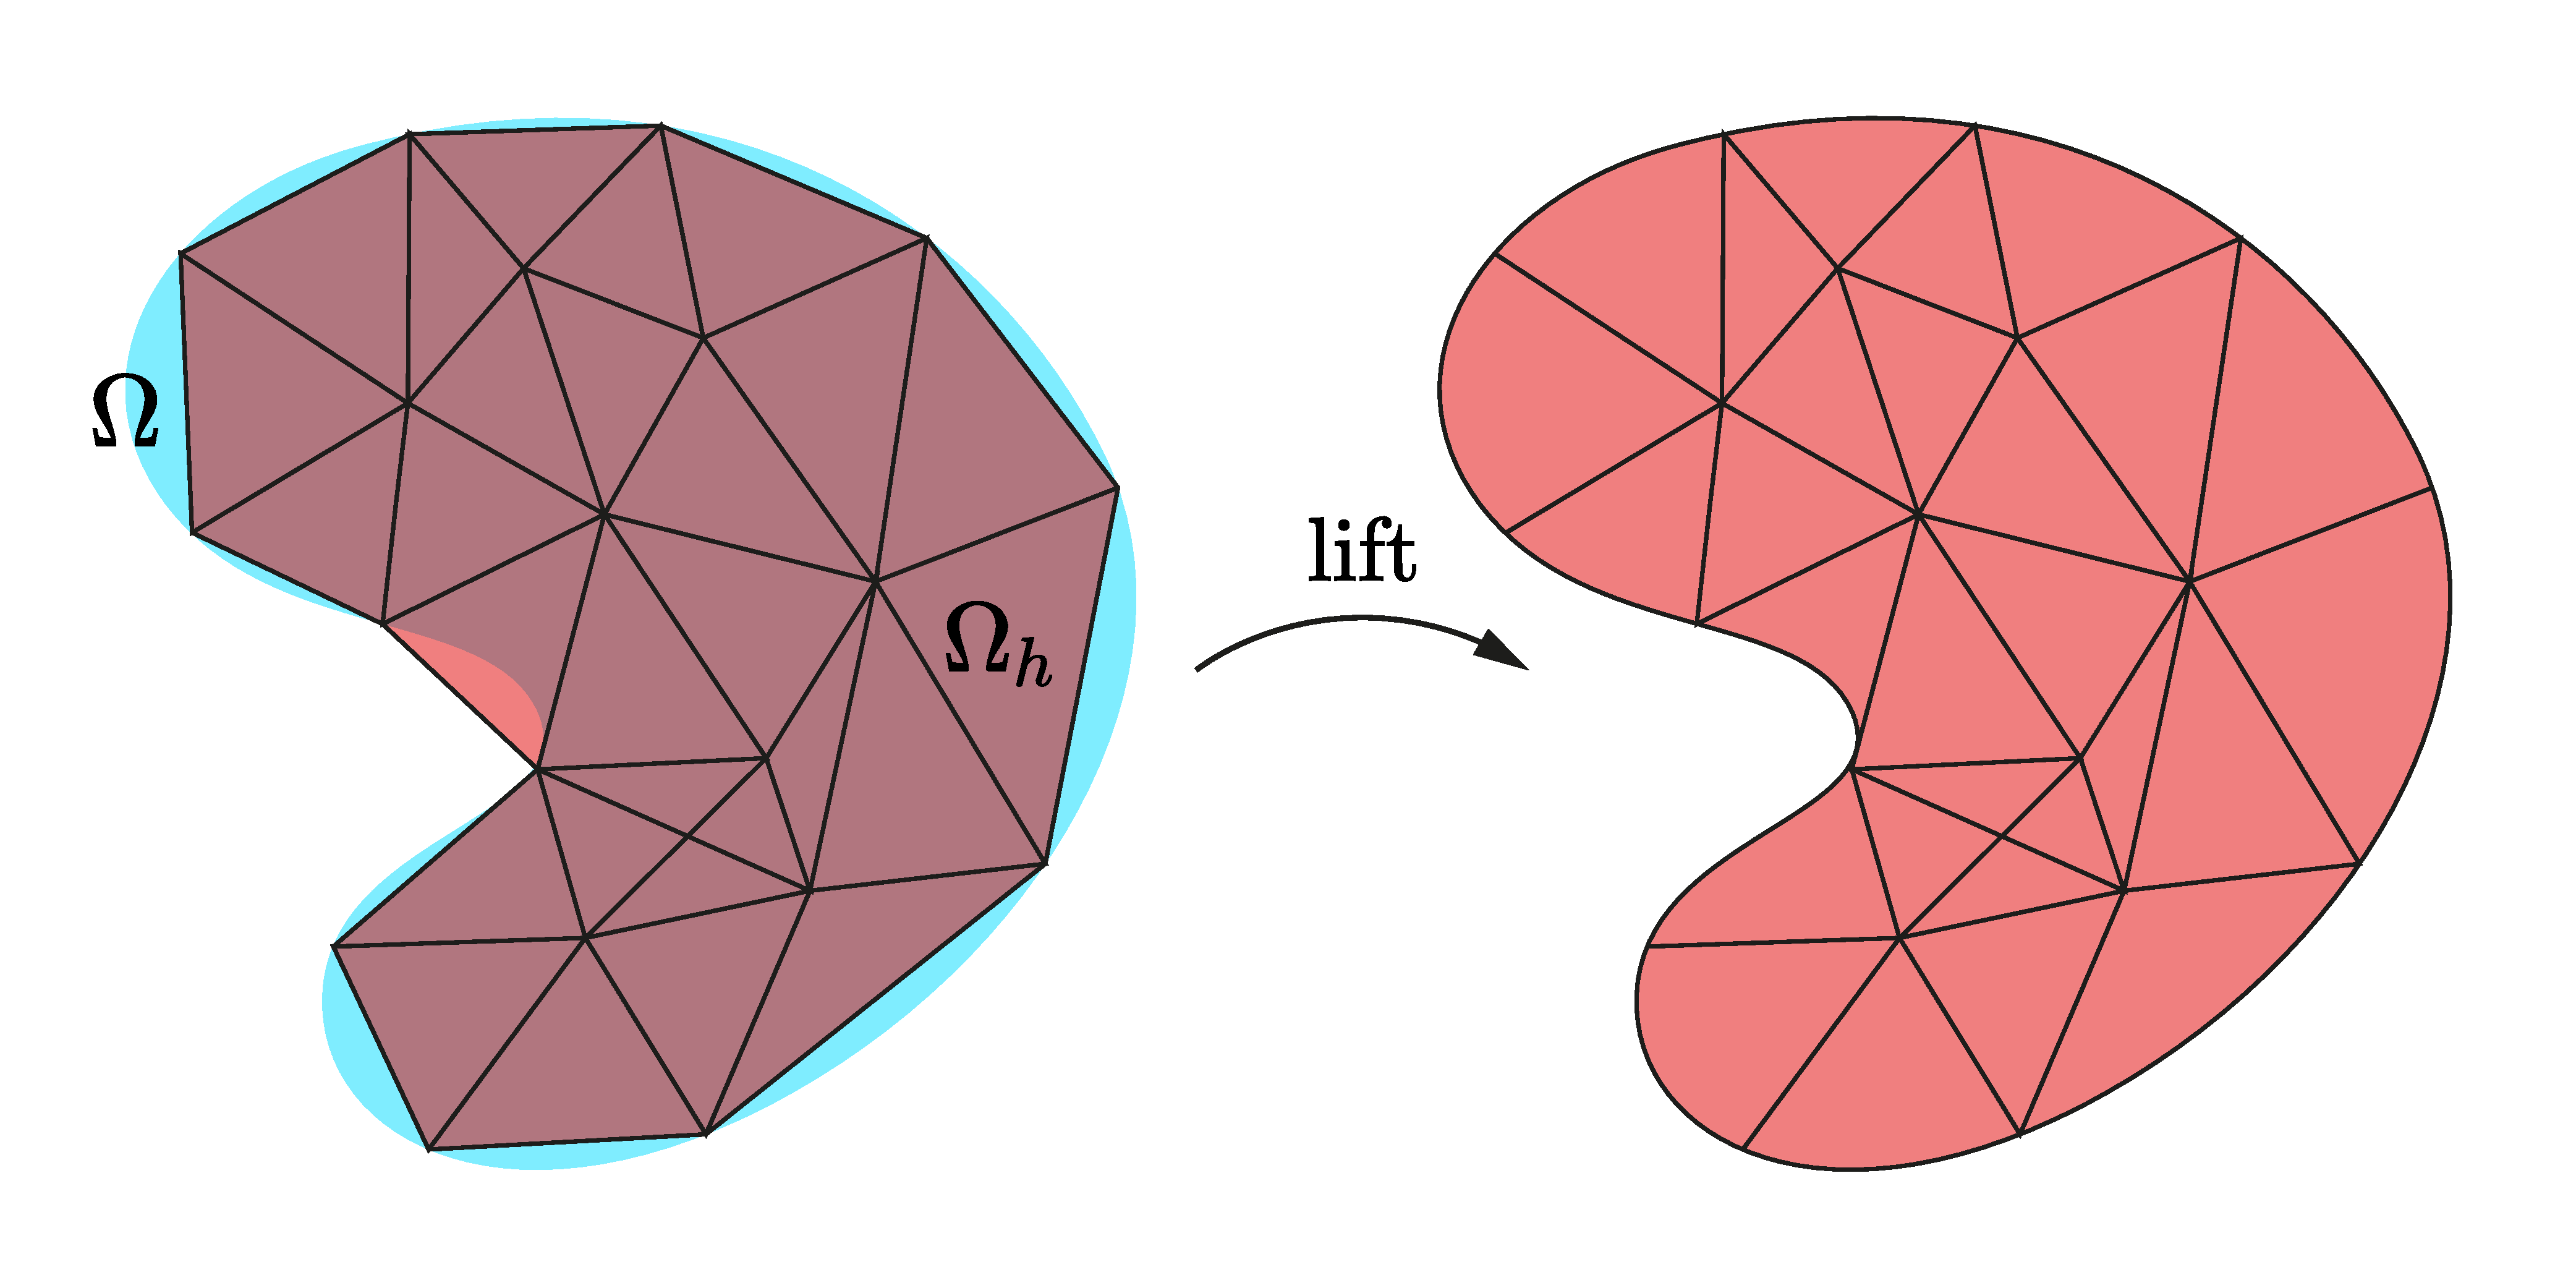
\includegraphics[width=0.65\columnwidth]{Images/Lift.pdf}
\caption{Lifting action}\label{fig:lift}
\end{figure}


\begin{obs}[$\tau$ and $\tau_h$]
\label{obs:tau_vs_tau_h}
\mbox{}\\
Throughout the rest of the chapter, we will derive several error estimates, which depend also on $\partial U$, hence, on $\tau$. We won't attempt to precisely track this dependency.
\mbox{}\\

% we won't try to take into account the fact that the reference domains $U_r$ and $U_{r,h}$ are changing under the actions of $\tau$ and $\tau_h$. It means that the estimates are $\tau, \tau_h$ dependent, but the dependence is not tracked. Therefore we will fix $U = \tau(U_r)$ and $U_h=\tau_h(U_{r,h})$ once and for all. 
 
Remember that \cref{ass:num_discr_shopt} must hold, which implies a specific form of $\tau_h$, i.e. that it must interpolate $\tau$. Given therefore a reference discretization $U_{r,h}$ interpolating $U_r$, then $\tau_h$, hence $U_h$, is completely determined by $\tau$. \mbox{}\\
Choosing such $U_{r,h}$ is not restrictive, but confining $\tau_h$ to be the interpolant of $\tau$, is: we refrain from generalizing our estimates to more arbitrary $\tau_h$, and we note that our result may be a first step of a more general argument (just like in finite element error estimates, the error between exact and discretized solution is decomposed into two parts by the introduction of a suitable interpolant).  \mbox{}\\

%Also note that 

This is in any case a novelty with respect to e.g. \cite{paganini}, which contains similar estimates to the ones we are about to derive, but in which $H^2$ regularity is demanded on non-convex polygonal domains. \mbox{}\\
\end{obs}


We now state the needed error estimates for states and adjoints of \cref{pb:uni_state_adj} when employing the optimize-then-discretize schemes of \cref{pb:num_scheme_recall}.


\begin{prop}[Optimize-then-discretize approximation of state and adjoint equations]
\label{prop:o-t-d}
Let \cref{ass:num_discr_shopt} be fulfilled. Then:

\begin{align*}
\sup_{t \in I }\norm{u(t)-u_h^l(t)}_{L^2(U)} + h\sqrt{\int_0^T\norm{u-u_h^l}^2_{H^1(U)}}\lesssim h^2	\\
\sup_{t \in I }\norm{a(t)-a_h^l(t)}_{L^2(U)} + h\sqrt{\int_0^T\norm{a-a_h^l}^2_{H^1(U)}} \lesssim h^2	\\
	\sup_{k=0,...,K}\norm{u_h(t^k)-u_h^k}_{L^2(U)}+\sqrt{\delta t \sum_{k=0}^{K-1} \norm{\theta(u_h(t^{k+1}) - u_h^{k+1}) + (1-\theta)(u_h(t^{k}) - u_h^{k})}_{H^1(U)}^2} \lesssim (\delta t)^{1/\theta}\\
	\sup_{k=0,...,K}\norm{a_h(t^k)-a_h^k}_{L^2(U)}+\sqrt{\delta t \sum_{k=1}^{K} \norm{\te(a_h(t^{k}) - a_h^{k}) + (1-\theta)(a(t^{k-1}) - a_h^{k-1})}_{H^1(U)}^2} \lesssim (\delta t)^{1/\theta}
\end{align*}

For the states, we will also need:

\begin{align*}
\sqrt{\int_0^T\norm{\partial_tu - (\partial_t u_h)^l}^2_{L^2(U)}}\lesssim h\\
\sqrt{\delta t \sum_{k=0}^{K-1} \norm{\frac{u_h(t^{k+1})-u_h(t^k)}{\delta t} - \frac{u_h^{k+1}-u_h^{k}}{\delta t}}_{L^2(U_h)}^2}\lesssim (\delta t)^{1/\theta}
\end{align*}
\end{prop}

%Note, the Dirichlet boundary varies between $v,w$. So, for $v$, $H^1_{0,D}=H^1_0$, whereas for $w$ we have $H^1_{0,D}=H^1_{0,m}=\{u \in H^1, u(\Gamma_m)=0\}$.

\begin{mproof}

The proposition is just a recollection of the results from \cref{chap:inh_fem} (namely \cref{prop:d_vd_sd}, \cref{thm:semidiscrete_error_bound}, \cref{cor:L2_deriv_est}, \cref{prop:another_bound}): we need to show that \cref{ass:num_discr_shopt} guarantees the validity of the hypothesis under which those results hold, and then to bound the constants $A,B,C,D,E$ that appear therein, uniformly on $\delta t$ and $h$. Since performing these tasks is not particularly enlightening, we only report the main steps to be performed. We do not track the dependency on the domain $U$ as already remarked.



%We show the satisfaction of all the hypothesis necessary to obtain \cref{thm:fully_discr_est_par} (where we track from there all the necessary assumptions), and then bound the constants therein, uniformly with respect to the space/time discretization. We do this for $u$ at first, then for $a$. We do not track the dependency on the domain $U$ as already remarked.
% This is just a more detailed repetition of the proof of the more general result \cref{cor:actual_par_est}.

The hypothesis which need to be verified are \cref{ass:discr_reg}, \cref{ass:smoothness_par_discr}, \cref{ass:basic_par_mix} and \cref{ass:full_discr_smoothness}.

We note at first that in the star-shaped setting, $\partial U \in C^2$ can be ensured by \cref{prop:Co_domain}.
%, which covers the geometry part of \cref{ass:discr_reg}.

\underline{States}

Hypothesis $1$ to $3$ guarantee that $u \in H^1(I,H^2(U))$ (by \cref{thm:mix_reg}, which we apply with $k=1$). This is \cref{ass:smoothness_par_discr}. The other hypothesis follow directly from $1-3$.

The constants $A,B,C,D,E$ for $u$ are also easily bounded employing $1-3$: in particular, no volumetric source terms are present, and all the compatibility ``residuals" $\delta_h^{(k)}(0)$ are $0$, $k=1,...,1/\te$ (see \cref{prop:d_vd_sd} for the notation).

\underline{Adjoints}

We can re-use the reasonings done for the states. There are of course some peculiarities for the adjoints.

Indeed, we also need the conditions on $\eta(T), \eta'(T)$ (point $4$) when applying \cref{thm:mix_reg} to obtain $a \in H^1(I,H^2(U))$, and also when ensuring that the compatibility ``residuals" $\delta_h^{(k)}(0)$ for the adjoints, $k=1,...,1/\te$, are bounded uniformly with respect to $h$.

Moreover, the adjoint equations have non trivial source terms like $\eta(v-w)$, $\eta(v_h-w_h)$ and $\eta(t^k)(v_h^k-w_h^k)$. By the results that we now know hold for the states (again, \cref{prop:d_vd_sd}, \cref{thm:semidiscrete_error_bound}, \cref{cor:L2_deriv_est}, \cref{prop:another_bound}), we know that $\eta(v-w)\simeq\eta(v_h-w_h)\simeq \eta(t^k)(v_h^k-w_h^k)$, so that we can satisfy all the requirements on these right hand sides of the adjoint equations. 
\end{mproof}

%\underline{Smoothness of $u$: \cref{ass:smoothness_par_discr} and  \cref{ass:basic_par_mix}}: we need to guarantee that $u \in H^1(I,H^2(U))$. To do so we turn to \cref{thm:mix_reg}, which we apply with $k=1$. Hypothesis $1$ to $3$ suffice for this.
%
%\underline{Assumptions for spatial semidiscretization of $u$: \cref{ass:discr_reg}}: they are also satisfied by $1-3$.
%
%\underline{Assumptions for full discretization of $u$: \cref{ass:full_discr_smoothness}}: the smoothness of the problem data is ensured by point $2$. We turn to the compatibility conditions of order $1,...,1/\theta$. The compatibility "residuals" $\delta_h^{(k)}(0)$ are all $0$ (see \cref{ass:full_discr_smoothness} for the notation) by hypothesis $3$, so that the compatibility relations are satisfied.
%
%\underline{Bounding the constants $A,B,C,D$ of $u$: \cref{thm:fully_discr_est_par}}: to bound $A,B$ uniformly with respect to $h$ we only need to note that the equation for $u$ has no source term. To bound $C$, this last fact, together with $\delta_h^k(0)=0$, $k=0,...,1/\theta$, suffices. $D=0$, in turn.
%
%We now turn verify the same facts for the adjoint states $a$.

%\underline{Smoothness of $a$}: we need to ensure that $a \in H^1(I,H^2(U))$. To apply \cref{thm:mix_reg} with $k=1$ we see that $\eta(T)(v(T)-w(T))$ should be zero on the Dirichlet boundary, which it is, given the fact that $\eta(T)=0$. We also need $v,w$ (so, generically, $u$), to be $H^1(I, L^2(U))$, which we have already checked (we even have $u \in H^1(I,H^2(U))$; \cref{ass:basic_par_mix} is also easily verified.
%
%\underline{Assumptions for spatial semidiscretization of $a$}: to fulfill \cref{ass:discr_reg} we see by the triangle inequality that $\norm{\eta(u-u_h^l)}_{L^2(U)}\lesssim C_u h^2$ would suffice, for a suitable $C_u$ (see \cref{ass:discr_reg} for the definition of $C_u$). Actually, given the properties of $\eta$, only $\norm{u-u_h^l}_{L^2(U)}\lesssim C_u h^2$ has to be asked. But the hypothesis we have verified for $u$ were sufficient for the conclusions of \cref{thm:semidiscrete_error_bound} to hold. We can therefore take $C_u = A = A(u)$, which is a constant in space and time, independent of $\delta t$ and $h$, as we saw before.
%
%\underline{Assumptions for full discretization of $a$}: the compatibility conditions listed in \cref{ass:full_discr_smoothness} are satisfied as long as $\eta(T)=0$ in the case $\theta = 1$, and additionally $\eta'(T)=0$ in the case $\theta=1/2$. We also have $u_h \in H^{1/\theta}(I,S^1_h)$ by $2$.
%
%\underline{Bounding the constants $A(a),B(a),C(a),D(a)$ of $a$}: this would be the last step to ensure the thesis of \cref{thm:fully_discr_est_par}, for $a$. Starting from $D(a)^2$, we see, thanks to the boundedness of $\eta$, that $D(a)^2 \lesssim \delta t \sum_{k=0}^{K-1}\norm{\theta(u_h(t^{k+1})-u_h^{k+1}) + (1-\theta)(u_h(t^k)-u_h^k)}^2_{L^2(U_h)}$. This is $O(\delta t^{2/\theta})$ by \cref{prop:d_vd_sd} and the above reasonings ($D=D(u)=0$, $C=C(u)$ is bounded uniformly).
%
%Moving on to $C(a)$. By the triangle inequality, the already checked compatibility relations and the boundedness of $\eta$, we see that there only remains to bound  the term $\ds \int_I\norm{u_h^{1/\theta}}_{-1,h}^2\lesssim \int_I\norm{u_h^{1/\theta}}_{L^2(U_h)}^2$. This can be done as above \cref{eqn:dd_est}.
%
%To bound $A(a)$ (equivalently $B(a)$), we need to check the boundedness of $\ds \int_I C_{\eta(v-w)}^2 + \int_I \norm{\eta(v_h - w_h)}_{H^1(U_h)}^2$ (the definition of $C_{\eta(v-w)}$ comes directly from \cref{ass:discr_reg}). In fact, we have chosen $\eta(v_h - w_h) \in S^1_h$ as a right hand side for the semidiscrete equation of $a_h$. A triangle inequality and basic stability estimates yield a bound for the second term. $C_{\eta(v-w)}$, thanks to \cref{thm:semidiscrete_error_bound}, is dominated by $A(v)+A(w)$, which we have in turn already estimated.

%\underline{The last estimate}
%
%Is the content of \cref{prop:another_bound}, where the constant $E$ can be bounded by the data as above, and the source terms $f_h^k$ are all zero.


Only for $\te = 1$, we now define a fully discrete shape optimization problem. This is necessary to justify that optimization and discretization commute when the implicit Euler method is used.



\begin{pb}[Discrete shape optimization problem]
\label{pb:discr_shopt}
As before, given a polygonal/polyhedral reference domain $U_{r,h}$ and transformations $\tau_h$ (vector valued finite element fields that preserve the discrete fixed boundary $\Gamma_{f,h}$), we solve:

$$\inf_{\tau_h }\frac{\delta t}{2}\sum_{k=1}^{K}\norm{v_h^k-w^k_h}_{L^2(\tau_h(U_{r,h}))}^2=:J_{h,\delta t}(\tau_h)$$


where $v_h^k, w^k_h$ are defined in \cref{pb:num_scheme_recall}, and their dependence on $\tau_h$ is not highlited in the notation. We also ask $\tau_h$ to have small enough $W^{1,\infty}$ norm, so as to keep $U_h = \tau_h(U_{r,h})$ bounded Lipschitz and preserve the mesh quality.

\end{pb}


\begin{prop}[Discrete shape gradient]
\label{prop:discrete_shape_gradient}
The discrete shape gradient of \cref{pb:discr_shopt} is:

\begin{align*}
	J_{h,\delta t}'(\tau_h)[\delta \theta_h] =\\
	\delta t \sum_{k=1}^{K} \left (\frac{w_h^{k}-w_h^{k-1}}{\delta t}, \dive(\delta \theta_h \circ \tau_h^{-1}) q_h^{k-1} \right )_{L^2(\tau_h(U_{r,h}))} + \delta t \sum_{k=1}^{K} (A'(\delta \theta_h \circ \tau_h^{-1}) \nabla w_h^k, \nabla q_h^{k-1})_{L^2(\tau_h(U_{r,h}))}+\\
	\delta t \sum_{k=1}^{K} \left (\frac{v_h^{k}-v_h^{k-1}}{\delta t}, \dive(\delta \theta_h \circ \tau_h^{-1}) p_h^{k-1} \right )_{L^2(\tau_h(U_{r,h}))} + \delta t \sum_{k=1}^{K} (A'(\delta \theta_h \circ \tau_h^{-1}) \nabla v_h^k, \nabla p_h^{k-1})_{L^2(\tau_h(U_{r,h}))}+\\
	\frac{\delta t}{2} \sum_{k=1}^{K} \int_{\tau_h(U_{r,h})} \eta(t^k)|v_h^k-w_h^k|^2  \dive(\delta \theta_h \circ \tau_h^{-1})
\end{align*}

Again, we dropped the dependence of $v,w$ on $\tau_h$, for simplicity. With unified notation as in \cref{pb:uni_state_adj}, the adjoint state $a_h^k \in S^1_{0,D,h}$ to $u_h^k$, $k=0,...,K$, satisfies:

\begin{pb}[Discrete adjoint states]

\begin{align*}
	\left ( \frac{a_h^{k-1}-a_h^k}{\delta t}, \phi_h\right )_{L^2(\tau_h(U_{r,h}))} + (\nabla a_h^{k-1}, \nabla a_h )_{L^2(\tau_h(U_{r,h}))} = \\(-1)^{\left [ u_h^k = v_h^k\right ]} \eta(t^k)(v_h^k-w_h^k,\phi_h)_{L^2(\tau_h(U_{r,h}))}, \quad 1\leq k \leq K\\
	p_h^K=0 
\end{align*}
%
%and 
%
%\begin{align*}
%	\left ( \frac{q_h^{k-1}-q_h^k}{\delta t}, v_h\right )_{L^2(\tau_h(U_{r,h}))} + (\nabla q_h^{k-1}, \nabla v_h )_{L^2(\tau_h(U_{r,h}))} - \eta(t^k)(v_h^k-w_h^k,v_h)_{L^2(\tau_h(U_{r,h}))} = 0, \quad 1\leq k \leq K\\
%	q_h^k = 0 \text{ on } \tau_h (\Gamma_{D,h,r}), \quad 1\leq k \leq K\\
%	q_h^K=0 
%\end{align*}

for $v_h \in  S^1_{0,D,h}$.

\end{pb}

\end{prop}

\begin{mproof}[Proof]
It can be done similarly to \cref{prop:sd_shopt}.
\end{mproof}


We now give a quantitative estimate of the approximation power of the discrete adjoints we just obtained. This is needed, because the scheme they satisfy is not exactly the implicit Euler treated in \cref{pb:num_scheme_recall}.

\begin{prop}[Error estimates for adjoint states in a discretize-then-optimize fashion]
\label{prop:d-t-o_estimates}
The discretize-then-optimize adjoints with implicit Euler from \cref{prop:discrete_shape_gradient} satisfy the same asymptotic, optimal order error estimates of \cref{prop:o-t-d}, under the same assumptions.
\end{prop}

\begin{mproof}
The proof is exactly that of \cref{prop:o-t-d}. The only difference comes from the fact that the right hand sides of the fully discrete adjoint equations are not ``correct", i.e. they are shifted by $\delta t$. But this is not an issue, as we shall now show. 

We see that we only need to show a bound of  $\delta t \sum_{k=1}^{K}\norm{\eta(t^{k-1})u_h(t^{k-1})-\eta(t^k)u_h^{k}}^2_{L^2(U_h)}$, where $u$ denotes the generic state corresponding state to the generic adjoint $a$ (this is the same notation as in the proof of \cref{prop:o-t-d}), and where $U_h=\tau_h(U_{r,h})$.

Applying the triangle inequality and using again the proof of \cref{prop:o-t-d}, we see that we actually only need to bound the term:

\begin{align*}
\delta t \sum_{k=1}^{K}\norm{\eta(t^{k-1})u_h(t^{k-1})-\eta(t^k)u_h^k}^2_{L^2(U_h)}\lesssim\\
\underbrace{\delta t \sum_{k=1}^{K}\norm{\eta(t^{k-1})(u_h(t^{k-1})-u_h(t^{k}))}^2_{L^2(U_h)}}_{\circled{1}}+
\underbrace{\delta t \sum_{k=1}^{K}\norm{(\eta(t^{k-1})-\eta(t^k))u_h(t^{k})}^2_{L^2(U_h)}}_{\circled{2}}+\\
\underbrace{\delta t \sum_{k=1}^{K}\norm{\eta(t^k)(u_h^k-u_h(t^k)))}^2_{L^2(U_h)}}_{\circled{3}}
\end{align*}

There holds $\ds  \circled{2} \leq \norm{\eta'}_\infty^2 \delta t^3 \sum_{k=1}^{K}\norm{u_h(t^{k})}^2_{L^2(U_h)}$. Call $\pi u_h := u_h(t^{k})$ for $t \in (t^k, t^{k+1})$. By \cref{lemma:pw_constant_appr} we see that, for $\delta t $ small enough, one has $\norm{\pi u_h}_{L^2(I, L^2(U_h))} \lesssim \norm{u_h}_{H^1(I,L^2(U_h))}$. This yields:

\begin{align*}
	 \ds  \circled{2}\leq \norm{\eta'}_\infty^2 \delta t^3 \sum_{k=1}^{K}\norm{u_h(t^{k})}^2_{L^2(U_h)}  = \norm{\eta'}_\infty^2 \delta t^2 \int_I \norm{\pi_h u_h}^2_{L^2(U_h)}\lesssim \delta t^2 \norm{u_h}_{H^1(I,L^2(U_h))}^2 \norm{\eta'}_\infty ^2
\end{align*}

On the other hand,  $\ds  \circled{1} \leq \norm{\eta}_\infty^2 \delta t \sum_{k=1}^{K}\norm{u_h(t^{k-1})-u_h(t^{k})}^2_{L^2(U_h)}$, and upon using the fundamental theorem of calculus, we conclude $\ds \circled{1} \leq \norm{\eta}_\infty^2 \delta t \sum_{k=1}^{K} \delta t \int_{I_k}\norm{u_h'}_{L^2(I_k , L^2(U_h))}^2$.

In both $\circled{1},\circled{2}$, $\norm{u_h}_{H^1(I,L^2(U_h))}^2$ can be bounded, uniformly with respect to $h$ (and $\delta t$), by suitable stability estimates which can be proved using the techniques of \cref{sec:pdes}.

It is clear from this estimate that a very steep $\eta$ may yield higher discretization errors.

Finally, by \cref{prop:o-t-d}, we obtain $\ds \circled{3} \lesssim (h^2+\delta t)\norm{\eta}_\infty^2 $.
\end{mproof}

\begin{obs}[Optimization and discretization commute]
\mbox{}\\
So, optimization and discretization commute, for $\theta=1$, and the perturbed implicit Euler method of \cref{prop:discrete_shape_gradient}, applied to the adjoints, is a ``legitimate" scheme, as we have just shown in \cref{prop:d-t-o_estimates}).
With a diagram:

\[\begin{tikzcd}
	&&& \text{\cref{prop:gateaux_diff}} \\
	\text{\cref{pb:shopt}} &&&&&& \text{\cref{prop:discrete_shape_gradient}}  \\
	&&& \text{\cref{pb:discr_shopt}} 
	\arrow["{\text{optimization}}"', from=3-4, to=2-7]
	\arrow["{\text{discretization}}", from=1-4, to=2-7]
	\arrow["{\text{optimization}}", from=2-1, to=1-4]
	\arrow["{\text{discretization}}"', from=2-1, to=3-4]
\end{tikzcd}\]


\end{obs}


%Before studying how well the discrete gradient approximates the continuous gradient, we need some additional error bounds for the state discretization. We do so to relax the smoothness requirements on the deformation field $\delta \theta$ in which the gradient is evaluated, in the upcoming arguments.
% This however entails assuming stronger compatibility relations for the state equations. From the physical point of view, this is not an issue: the state equations, unlike the adjoint ones, coming from a physical process, should naturally satisfy such compatibility. 

%The following proposition in particular is proven in this section, applied to our concrete (state) equations. The proof also applies to the general case, of course, under suitable assumptions.

%\begin{thm}[Fully discrete estimate for shape gradients, implicit Euler case]
%\label{thm:ie_shape_grad_est}
%Let  $U$ be fixed and $U_h$ as in \cref{ass:num_discr_shopt}. The same assumption must hold. Let $\delta \te \in W^{1,\infty}(U)$ and $\delta \te_h$ be a vector valued finite element function of $S^1_h=S^1_h(U_h)$. There exists a constant $\gamma$ that depends on $U$, the shape regularity and quasi-uniformity of the meshes, independent of $h, \delta t$, such that, for $h,\delta t$ small enough, we have:
%
%\begin{align*}
%|J'(	U)[\delta \te]-J'_{h,\delta t}(U_h)[\delta \te_h]|\leq \gamma\left [ (h+\delta t)(\norm{\delta \te}_{W^{1,\infty}(U)}+\norm{\delta \te_h}_{W^{1,\infty}(U_h)}) + \norm{\delta \te - \delta \te_h^l}_{W^{1,\infty}(U)}\right ]
%\end{align*}
%
%where the notation $J'(U)[\delta \te]:=J'(\tau)[\delta \te\circ \tau]$, if $U=\tau(U_r)$, is to emphasize that the dependence on $\tau$ is not tracked.
%Analogously $J'_{h,\delta t}(U_h)[\delta \te]:=J'_{h,\delta t}(\tau_h)[\delta \te_h\circ \tau]$, with $U_h = \tau_h(U_{r,h})$ and a suitable $\tau_h$ that(linearly) interpolates $\tau$ on the spatial discretization nodes.
%
%\end{thm}
%\begin{mproof}
%
%\underline{Forewarning}
%
%As we have already mentioned in \cref{obs:tau_vs_tau_h}, we consider $U, U_h$ to be frozen in our estimate, and we assume $U_h$ to be interpolating $U$, as in \cref{ass:num_discr_shopt}. For simplicity, we are also considering $\delta \theta$ and $\delta \theta_h$ to be defined on the moving domain. We again recover the notation $u, a$ to indicate a state and its correspondent adjoint (so, $u=v \iff a = p$ or $u=w \iff a = q$). Therefore, the quantities to be compared become, thanks to \cref{prop:gateaux_diff} and \cref{prop:discrete_shape_gradient}:
%%
%%\begin{align*}
%%	\delta t \sum_{k=1}^{K} \left (\frac{w_h^{k}-w_h^{k-1}}{\delta t}, \dive(\delta \theta_h ) q_h^{k-1} \right )_{L^2(U_h)} + \delta t \sum_{k=1}^{K} (A'(\delta \theta_h ) \nabla w_h^k, \nabla q_h^{k-1})_{L^2(U_h)}+\\
%%	\delta t \sum_{k=1}^{K} \left (\frac{v_h^{k}-v_h^{k-1}}{\delta t}, \dive(\delta \theta_h ) p_h^{k-1} \right )_{L^2(U_h)} + \delta t \sum_{k=1}^{K} (A'(\delta \theta_h) \nabla v_h^k, \nabla p_h^{k-1})_{L^2(U_h)}+\\
%%	\frac{\delta t}{2} \sum_{k=1}^{K} \int_{U_h} \eta(t^k)|v_h^k-w_h^k|^2  \dive(\delta \theta_h )\\
%%\end{align*}
%%
%%and
%%
%%\begin{align*}
%%	\int_I (w_t \dive(\delta \te), q)_{L^2(U)}+ \int_I (A'(\delta\te )\nabla v, \nabla p)_{L^2(U)}+\\
%%\int_I (v_t\dive(\delta \te), p)_{L^2(U)}+ \int_I (A'(\delta\te )\nabla w, \nabla q)_{L^2(U)}+\\
%%\frac{1}{2}\int_I\int_{U}\eta |v-w|^2\dive(\delta \te)
%%\end{align*}
%%
%%To make a fair comparison we also need to have $\delta \te $ and $\delta \te_h$ to be somewhat related. We will discuss in the end some possible choices.
%%
%%\underline{Splitting into pieces}
%
%%We separately bound the five pieces, which, if we again recover the notation $u, a$ to indicate a state and its correspondent adjoint (so, $u=v \iff a = p$ or $u=w \iff a = q$), means to find bounds just for the following three quantities:
%
%\begin{align*}
%	\circled{$\partial$}:=\delta t \sum_{k=1}^{K} \left (\frac{u_h^{k}-u_h^{k-1}}{\delta t}, \dive(\delta \theta_h ) a_h^{k-1} \right )_{L^2(U_h)}  - \int_I (u_t , \dive(\delta \te) a)_{L^2(U)}
%\end{align*}
%
%\begin{align*}
%	\circled{$\nabla$} := \delta t \sum_{k=1}^{K} (A'(\delta \theta_h ) \nabla u_h^k, \nabla a_h^{k-1})_{L^2(U_h)} - \int_I (A'(\delta\te )\nabla u, \nabla a)_{L^2(U)}
%\end{align*}
%
%\begin{align*}
%	\circled{J}:=\frac{\delta t}{2} \sum_{k=1}^{K} \int_{U_h} \eta(t^k)|v_h^k-w_h^k|^2  \dive(\delta \theta_h ) - \frac{1}{2}\int_I\int_{U}\eta |v-w|^2\dive(\delta \te)
%\end{align*}
%
%\underline{Derivatives: rewriting}
%
%Denote again by $\pi a = a(t^k)$ on $(t^k,t^{k+1})$. Then:
%
%\begin{align*}
%	\circled{$\partial$}=\underbrace{- \int_I (u_t , \dive(\delta \te) (a -\pi a))_{L^2(U)}}_{\circled{1}}+ \underbrace{\delta t \sum_{k=1}^{K} \left (\frac{u_h^{k}-u_h^{k-1}}{\delta t}, \dive(\delta \theta_h ) a_h^{k-1} \right )_{L^2(U_h)} - \int_I (u_t , \dive(\delta \te) \pi a)_{L^2(U)}}_{\circled{R1}}
%\end{align*}
%
%Now:
%
%\begin{align*}
%	\circled{R1} = \delta t \sum_{k=1}^{K} \left (\frac{u_h^{k}-u_h^{k-1}}{\delta t}, \dive(\delta \theta_h ) a_h^{k-1} \right )_{L^2(U_h)} - \delta t \sum_{k=1}^{K}\left (\frac{u(t^{k})-u(t^{k-1})}{\delta t} , \dive(\delta \te)  a(t^{k-1})\right )_{L^2(U)}=\\
%\underbrace{- \delta t \sum_{k=1}^{K}\left (\frac{u(t^{k})-u(t^{k-1})}{\delta t} -\frac{u^{k,l}_h-u^{k-1,l}_h}{\delta t} , \dive(\delta \te)  a(t^{k-1})\right )_{L^2(U)}}_{\circled{2}}+\\ \underbrace{\delta t \sum_{k=1}^{K} \left (\frac{u_h^{k}-u_h^{k-1}}{\delta t}, \dive(\delta \theta_h ) a_h^{k-1} \right )_{L^2(U_h)}- \delta t \sum_{k=1}^{K}\left (\frac{u^{k,l}_h-u^{k-1,l}_h}{\delta t} , \dive(\delta \te)  a(t^{k-1})\right )_{L^2(U)}}_{\circled{R2}} 
%\end{align*}
%
%Lastly:
%
%\begin{align*}
%	\circled{R2} = \underbrace{\delta t \sum_{k=1}^{K} \left (\frac{u_h^{k}-u_h^{k-1}}{\delta t}, \dive(\delta \theta_h ) a_h^{k-1} \right )_{L^2(U_h)}
%		- \delta t \sum_{k=1}^{K}\left (\frac{u^{k,l}_h-u^{k-1,l}_h}{\delta t} , \dive(\delta \te_h^l)  a_h^{k-1,l}\right )_{L^2(U)} }_{\circled{3}}+ \\
%	\underbrace{- \delta t \sum_{k=1}^{K}\left (\frac{u^{k,l}_h-u^{k-1,l}_h}{\delta t} , (\dive(\delta \te) - \dive(\delta \te_h^l)  )a_h^{k-1,l}\right )_{L^2(U)}}_{\circled{4}} + \underbrace{- \delta t \sum_{k=1}^{K}\left (\frac{u^{k,l}_h-u^{k-1,l}_h}{\delta t} , \dive(\delta \te) \left(a(t^{k-1})-a_h^{k-1,l}\right)\right )_{L^2(U)}}_{\circled{5}}
%\end{align*}
%
%\underline{Derivatives: estimation}
%
%We start with $\circled{1},\circled{2},\circled{5}$.
%
%We have, by the Cauchy-Schwarz inequality and \cref{lemma:pw_constant_appr}:
%
%\begin{align*}
%\left |\circled{1}\right|\leq \delta t \norm{\dive(\delta \te)}_{L^\infty(U)}\norm{u_t}_{L^2(I,L^2(U))}\norm{a'}_{L^2(I,L^2(U))}\lesssim \delta t \norm{\dive(\delta \te)}_{L^\infty(U)}
%\end{align*}
%
%Then, using again the Cauchy-Schwarz inequality:
%
%\begin{align*}
%\left |\circled{2}\right|\leq \norm{\dive(\delta \te)}_{L^\infty(U)} \sqrt{\delta t \sum_{k=0}^{K-1} \norm{a(t^k)}^2_{L^2(U)}}\sqrt{\delta t \sum_{k=0}^{K-1} \norm{\frac{u(t^{k+1})-u(t^k)}{\delta t} - \frac{u_h^{k+1,l}-u_h^{k, l}}{\delta t}}_{L^2(U)}^2}
%\end{align*}
%
%Employing \cref{prop:another_bound} at first, and \cref{lemma:pw_constant_appr} afterwards:
%
%\begin{align*}
%\left |\circled{2}\right|\lesssim (h+\delta t) \norm{\dive(\delta \te)}_{L^\infty(U)} \sqrt{\sum_{k=0}^{K-1} \int_{I_k}\norm{a(t^k)}^2_{L^2(U)}}\lesssim (h+\delta t) \norm{\dive(\delta \te)}_{L^\infty(U)} \norm{a'}_{L^2(I,L^2(U))}\lesssim  (h+\delta t) \norm{\dive(\delta \te)}_{L^\infty(U)}
%\end{align*}
%
%Note, this is where we used \cref{prop:another_bound}. One could alternatively assume higher differentiability for $\theta$ and proceed with \cref{prop:o-t-d}.
%
%Then:
%
%\begin{align*}
%	\left |\circled{5}\right|\leq  \norm{\dive(\delta \te)}_{L^\infty(U)} \sqrt{\delta t\sum_{k=0}^{K-1} \norm{\frac{u_h^{k+1,l}-u_h^{k, l}}{\delta t}}_{L^2(U)}^2}\sqrt{\delta t\sum_{k=0}^{K-1} \norm{a(t^{k})-a_h^{k,l}}_{L^2(U)}^2}
%\end{align*}
%
%Thanks to \cref{prop:d-t-o_estimates} we can write:
%
%\begin{align*}
%	\left |\circled{5}\right|\lesssim (h^2+\delta t)  \norm{\dive(\delta \te)}_{L^\infty(U)} \sqrt{\delta t\sum_{k=0}^{K-1} \norm{\frac{u_h^{k+1,l}-u_h^{k, l}}{\delta t}}_{L^2(U)}^2}
%\end{align*}
%
%Using \cref{prop:another_bound} and the last step of its proof:
%
%\begin{align*}
%	\left |\circled{5}\right|\lesssim (h^2+\delta t)  \norm{\dive(\delta \te)}_{L^\infty(U)}
%\end{align*}
%
%And with similar reasonings:
%\begin{align*}
%	\left |\circled{4}\right|\lesssim \norm{\dive(\delta \te) - \dive(\delta \te_h^l)}_{L^\infty(U)}
%\end{align*}
%
%Member $\circled{3}$ can be bound with the help of \cref{prop:lin_appr}.
%
%\underline{Gradients: rewriting}
%
%We have:
%
%\begin{align*}
%	\delta t \sum_{k=1}^{K} (A'(\delta \theta_h ) \nabla u_h^k, \nabla a_h^{k-1})_{L^2(U_h)} - \int_I (A'(\delta\te )\nabla u, \nabla a)_{L^2(U)} = \\
%	\underbrace{\delta t \sum_{k=1}^{K} (A'(\delta \theta_h ) \nabla u_h^k, \nabla a_h^{k-1})_{L^2(U_h)}- \int_I (A'(\delta\te )\nabla\tilde{\pi}u, \nabla \pi a)_{L^2(U)}}_{\circled{R3}} + \\\underbrace{- \int_I (A'(\delta\te )\nabla u, \nabla (a-\pi a))_{L^2(U)}}_{\circled{6}}\underbrace{- \int_I (A'(\delta\te )\nabla (u - \tilde{\pi}u), \nabla \pi a)_{L^2(U)}}_{\circled{7}} 
%\end{align*}
%
%Continuing the splitting:
%
%\begin{align*}
%\circled{R3} = \delta t \sum_{k=1}^{K} (A'(\delta \theta_h ) \nabla u_h^k, \nabla a_h^{k-1})_{L^2(U_h)} - \delta t \sum_{k=1}^{K} (A'(\delta\te )\nabla u(t^{k}) , \nabla a(t^{k-1}))_{L^2(U)} = \\
%\underbrace{\delta t \sum_{k=1}^{K} (A'(\delta \theta_h ) \nabla u_h^k, \nabla a_h^{k-1})_{L^2(U_h)} - \delta t \sum_{k=1}^{K} (A'(\delta\te_h^l )\nabla u_h^{k,l} , \nabla a_h^{k-1,l})_{L^2(U)}}_{\circled{8}}+
%- \underbrace{\delta t \sum_{k=1}^{K} ((A'(\delta \te) - A'(\delta\te_h^l ))\nabla u_h^{k,l} , \nabla a_h^{k-1,l})_{L^2(U)}}_{\circled{9}}+\\
%- \underbrace{\delta t \sum_{k=1}^{K} (A'(\delta\te )\nabla (u(t^{k})-u_h^{k,l}) , \nabla a(t^{k-1}))_{L^2(U)}}_{\circled{10}}+
%- \underbrace{\delta t \sum_{k=1}^{K} (A'(\delta\te )\nabla u_h^{k,l} , \nabla (a(t^{k-1}) -a_h^{k-1,l}))_{L^2(U)}}_{\circled{11}}
%\end{align*}
%\underline{Gradients: estimation}
%
%The terms $\circled{10}, \circled{11}$ can be estimated in a common way. We only need to make sure that $\ds \delta t \sum_{k=1}^{K} \norm{\nabla u_h^{k,l}}_{L^2(U)}^2 $ is bounded uniformly (true by \cref{prop:o-t-d}, \cref{lemma:pw_constant_appr} and the smoothness of $u$, ensured by \cref{ass:num_discr_shopt}), and also that $\ds \delta t \sum_{k=1}^{K} \norm{\nabla a(t^{k-1})}_{L^2(U)}^2$ is uniformly bounded (true by \cref{lemma:pw_constant_appr} and the smoothness of $a$, ensured by \cref{ass:num_discr_shopt}). Then an application of the Cauchy-Schwarz inequality, \cref{prop:d-t-o_estimates} and \cref{prop:o-t-d} yield:
%
%\begin{align*}
%	\left | \circled{10} \right |, \left |\circled{11}\right | \lesssim (h+\delta t) \norm{A'(\delta \te)}_{L^\infty(U)}
%\end{align*}
%
%Similarly:
%
%\begin{align*}
%	\left | \circled{9} \right | \lesssim (h+\delta t) \norm{A'(\delta \te_h^l)-A'(\delta \te)}_{L^\infty(U)}
%\end{align*}
%
%and the term $\circled{8}$ follows directly from \cref{prop:lin_appr}.
%
%\underline{Cost functions: estimation}
%
%We are missing a bound on: 
%
%\begin{align*}
%	\circled{J}:=\frac{\delta t}{2} \sum_{k=1}^{K} \int_{U_h} \eta(t^k)|v_h^k-w_h^k|^2  \dive(\delta \theta_h ) - \frac{1}{2}\int_I\int_{U}\eta |v-w|^2\dive(\delta \te) = \\
%	\underbrace{\frac{\delta t}{2} \sum_{k=1}^{K} \int_{U_h} \eta(t^k)|v_h^k-w_h^k|^2  \dive(\delta \theta_h ) - \frac{1}{2}\int_I\int_{U}\eta |v-w|^2\dive(\delta \te_h^l)}_{\circled{R4}}+
%	-\underbrace{ \frac{1}{2}\int_I\int_{U}\eta |v-w|^2(\dive(\delta \te) - \dive(\delta \te_h^l))}_{\circled{12}}
%\end{align*}
%
%We find:
%
%\begin{align*}
%	\left | \circled{12} \right | \lesssim \norm{\dive(\delta \te) - \dive(\delta \te_h^l)}_{L^\infty(U)}
%\end{align*}
%
%whereas:
%
%\begin{align*}
%\circled{R4} =\underbrace{ \frac{\delta t}{2} \sum_{k=1}^{K} \int_{U_h} \eta(t^k)|v_h^k-w_h^k|^2  \dive(\delta \theta_h ) - \frac{\delta t}{2} \sum_{k=1}^{K}\int_{U} \eta(t^k) |v_h^{k,l}-w_h^{k,l}|^2\dive(\delta \te_h^l)}_{\circled{13}}+\\
%\underbrace{\frac{\delta t}{2} \sum_{k=1}^{K}\int_{U} \eta(t^k) (|v_h^{k,l}-w_h^{k,l}|^2- |v(t^k)-w(t^k)|^2)\dive(\delta \te_h^l)}_{\circled{14}}+
%\underbrace{\frac{1}{2}\int_I\int_{U}\tilde{\pi} \eta (|\tilde{\pi} v-\tilde{\pi} w|^2-|v-w|^2)\dive(\delta \te_h^l)}_{\circled{15}}+
%\underbrace{\frac{1}{2}\int_I\int_{U}(\tilde{\pi} \eta - \eta) |v-w|^2\dive(\delta \te_h^l)}_{\circled{16}}
%\end{align*}
%
%For $\circled{16}$ we can use the fact that that $\norm{\eta -\tilde{\pi} \eta}_\infty\leq \delta t \norm{\eta'}_\infty$ to ensure that:
%
%\begin{align*}
%	\left | \circled{16} \right |\lesssim \delta t \norm{\dive(\delta \te_h^l)}_{L^\infty(U_h)}
%\end{align*}
%
%Similarly, also by applying the Cauchy-Schwarz' inequality and \cref{lemma:pw_constant_appr}:
%
%\begin{align*}
%	\left | \circled{15} \right |\lesssim  \norm{\dive(\delta \te_h^l)}_{L^\infty(U_h)} (\norm{v-\tilde{\pi} v}_{L^2(I,L^2(U))}+\norm{w-\tilde{\pi} w}_{L^2(I,L^2(U))})\lesssim \delta t \norm{\dive(\delta \te_h^l)}_{L^\infty(U_h)}
%\end{align*}
%
%The Cauchy-Schwarz' inequality also yields:
%\begin{align*}
%	\left | \circled{14} \right | \lesssim \norm{\dive(\delta \te_h^l)}_{L^\infty(U_h)}(E_v+E_w)(S_v+S_w)
%\end{align*}
%
%where $\ds E_u = \sqrt{\delta t \sum_{k=1}^{K}\norm{u(t^k)-u_h^{k,l}}_{L^2(U)}^2}$ and $\ds S_u = \sqrt{\delta t \sum_{k=1}^{K}\norm{u(t^k)+u_h^{k,l}}_{L^2(U)}^2} $.
%
%Through \cref{prop:o-t-d} we find $E_u \lesssim \delta t + h^2$, whereas \cref{prop:o-t-d} combined with \cref{lemma:pw_constant_appr} yield $S_u \lesssim 1$, so that:
%
%\begin{align*}
%	\left | \circled{14} \right | \lesssim (\delta t + h^2)\norm{\dive(\delta \te_h^l)}_{L^\infty(U_h)}
%\end{align*}
%
%
%Similarly, and reasoning as in \cref{prop:lin_appr}, we can also see that:
%
%\begin{align*}
%	\left | \circled{13} \right | \lesssim h \norm{\dive(\delta \te_h^l)}_{L^\infty(U_h)}
%\end{align*}
%
%This concludes the proof.
%\end{mproof}
%
%Upon choosing $\delta \te = \delta \te_h^l$ we easily obtain the following corollary.
%
%\begin{cor}
%\label{cor:ie_shape_grad_est}
%
%With the same hypothesis and notation of \cref{thm:ie_shape_grad_est}:
%
%\begin{align*}
%|J'(	U)[\delta \te_h^l]-J'_{h,\delta t}(U_h)[\delta \te_h]|\leq \gamma (h+\delta t)\norm{\delta \te_h}_{W^{1,\infty}(U_h)}
%\end{align*}
%
%\end{cor}



\section{Approximation of shape gradients}
\label{sec:d-t-o_IE}

In our numerical experiments (see \cref{chap:num_exp}) we adopt a discretize-then-optimize approach. When employing the implicit Euler method in time, optimization and discretization commute, as we have explained just above. We are moreover able to quantify the error generated when substituting the continuous shape gradient with the fully discretized one. 

A future line of research could be to extend such conclusions to the case of the Crank-Nicolson method, in a discretize-then-optimize setting, so as to fully justify the adopted algorithms in some of the numerical experiments we conducted. A promising direction would be to find a way to adapt the arguments of \cite{flaig} in our context of smooth geometries, at least to show commutativity of optimization and discretization. We will prove, as a partial replacement, optimize-then-discretize error estimates for the shape gradient.

These estimates are similar to those in \cite{paganini}, although formulated in a slightly different context: in a time-dependent setting, and with a more precise handling of the geometry mismatch. In \cite{paganini}, order $2$ estimates (in space) are obtained: this is because the deformation field $\delta \te$  in which the shape gradient is tested, is assumed to have two orders of differentiability, so that certain duality techniques may be employed. Such a result doesn't fully explain why superconvergence happens in the context of just $W^{1,\infty}$ displacements, a fact which is indeed observable in our experiments.

For smoother displacement fields $\delta \te\in W^{2,\infty}$, a similar superconvergence result for the shape gradient is available also in our context. This is shown initially for the spatial semidiscretization, and from here we speculate that such a result may be available also in the fully discrete case. This is also confirmed by the experiments in \cref{sec:experiments}. With regards to fully discrete estimates: in a commutative setting for the implicit Euler scheme, we are able to give full theoretical justification. In the Crank-Nicolson case, we could only arrive at non-commutative optimize-then-discretize estimates.

%The difference with the estimates of \cite{paganini} lies in the fact that we are explicitly taking into account the geometry discrepancy $U \neq U_h$ (in the special case that $U_h$ interpolates $U$), apart from the time dependent setting we are in.

If the displacement fields are not smooth enough, $O(h^2)$ orders, as noted in \cite{paganini}, don't seem to be so easily obtainable: we are also are able to only prove $O(h)$ estimates (but numerically observe an $O(h^2)$ order, see \cref{sec:experiments}).


\begin{thm}[Semidiscrete error estimates for shape gradient]
\label{thm:superconvergence_sd}
Let \cref{ass:num_discr_shopt} hold. There exists a constant $\gamma$ that depends on $U$, the shape regularity and quasi-uniformity of the meshes, but independent of $h$, such that, for $h$ small enough and for all $\delta \te \in W^{1+s,\infty}(U;\mR^n)$, $s=0,1$, we have:

\begin{align*}
	\left |J'(U)[\delta \te] - J'_h(U_h)[\delta \te^{-l}] \right|\leq \gamma  h^{1+s} \norm{\delta \te}_{W^{1+s,\infty}(U;\mR^n)}
\end{align*}

%If otherwise $\delta \te \in W^{1,\infty}(U;\mR^n)$, we obtain:
%
%\begin{align*}
%	\left |J'(U)[\delta \te] - J'_h(U_h)[\delta \te^{-l}] \right|\leq \gamma  h\norm{\delta \te}_{W^{1,\infty}(U;\mR^n)}
%\end{align*}

The notation $J'(U)[\delta \te]:=J'(\tau)[\delta \te\circ \tau]$, if $U=\tau(U_r)$, is to emphasize that the dependence on $\tau$ is not tracked.
Analogously $J'_{h}(U_h)[\delta \te]:=J'_{h,\delta t}(\tau_h)[\delta \te_h\circ \tau]$, with $U_h = \tau_h(U_{r,h})$ and a suitable $\tau_h$ that (linearly) interpolates $\tau$ on the spatial discretization nodes. Note that no assumptions on the boundary values of $\delta \te$ are made here.

\end{thm}

\begin{obs}
In the remaining proofs of this chapter, we apply stability estimates to bound the norms of discretized quantities independently of $h$, without explicitly writing this out in detail. Such estimates can be easily derived with the techniques of \cref{sec:pdes} and \cref{chap:inh_fem}. We refer to e.g. \cref{prop:wp_discr_par} and to the proof of \cref{prop:another_bound} for some hints in this direction. We also don't write the norms of the continuous quantities, because they don't depend on $h$ (or $\delta t$). Moreover, \cref{prop:lift} is used liberally to relate the norms of lifted and unlifted functions, and we will not mention every time it is invoked.
\end{obs}

\begin{mproof}[Proof for $\delta \te \in W^{1,\infty}$]
We compare ``time derivative" terms, ``gradient" terms and ``cost function" terms in the difference $\ds J'(U)[\delta \te] - J'_h(U_h)[\delta \te^{-l}]$, terms that come from \cref{prop:sd_shopt} and \cref{prop:gateaux_diff}, and use the estimates in \cref{prop:o-t-d} and \cref{prop:lin_appr} to bound every term like $\lesssim h \norm{\delta \te}_{W^{1,\infty}(U;\mR^n)}$. 

%, and use \cref{prop:lin_appr}, apart from the semidiscretization error estimates for the partial differential equations, to obtain an overall $O(h^2)$ term, or $O(h)$ term. For the expression of the semidiscretized shape gradient we make use of \cref{prop:sd_shopt}. We also call $\delta \te_h := \delta \te^{-l}$.

\underline{Time derivatives}

We recover the notation $u\rightarrow$ generic state ($v$ or $w$), $a\rightarrow$ adjoint state of $u$.
We have:

\begin{align*}
	\int_I(u',a\dive(\delta \te))_{L^2(U)}-\int_I (u_h',a_h\dive(\delta \te_h))_{L^2(U_h)}=\\
	\underbrace{\int_I((u-u_h^l)',a\dive(\delta \te))_{L^2(U)}}_{\circled{1}}+
	\underbrace{\int_I((u_h')^l, (a-a_h^l)\dive(\delta \te))_{L^2(U)}}_{\circled{2}}+\\
	\underbrace{\int_I((u_h')^l, a_h^l\dive(\delta \te))_{L^2(U)}-\int_I (u_h',a_h\dive(\delta \te^{-l}))_{L^2(U_h)}}_{\circled{3}}
\end{align*}

%	\underbrace{\int_I((u_h')^l, a_h^l(\dive(\delta \te) - \dive(\delta \te_h^l)))_{L^2(U)}}_{\circled{3'}}


We apply  \cref{prop:o-t-d} to $\circled{1}, \circled{2}$ to obtain $\ds  \left | \circled{1} \right |,  \left | \circled{2} \right | \lesssim h\norm{\dive{\delta \theta}}_{L^\infty(U)}$. Moreover, employing \cref{prop:lin_appr}, we find:

\begin{align*}
	\left | \circled{3} \right |\lesssim  h \norm{u_h'}_{L^2(I,L^2(U_h))}\norm{a_h}_{L^2(I,L^2(U_h))}\norm{\delta \te}_{W^{1,\infty}(U)} \lesssim  h \norm{\delta \te}_{W^{1,\infty}(U)}
\end{align*}
%It is crucial here that $\delta \te$ has two weak derivatives, so that $a\delta \te$ is as smooth as required by \cref{cor:deriv_est_semid}. Otherwise, we can only assume $\delta \te \in W^{1,\infty}$ and apply \cref{cor:L2_deriv_est}, which yields $\ds  \left | \circled{1} \right | \lesssim h\norm{\dive{\delta \theta}}_{L^\infty(U)}$.

%On the other hand, employing \cref{thm:semidiscrete_error_bound}, \cref{prop:lift} and suitable stability estimates to $u_h'$ (which are avaliable by \cref{ass:full_discr_smoothness}), we come as well to $\ds \left | \circled{2} \right | \lesssim h^2\norm{\dive{\delta \theta}}_{L^\infty(U)}$.



%Lastly, $\circled{3'}\ds \lesssim \norm{\delta \te - \delta \te_h^l}_{W^{1,\infty}(\mR^n; \mR^n)}$, where we applied \cref{prop:lift} and suitable stability estimates to bound $u_h'$ and $a_h$ in the $L^2(I,L^2)$ norm.


\underline{Gradients}

We perform the splitting:

\begin{align*}
	\int_I (A'(\delta\te )\nabla u, \nabla a)_{L^2(U)}-\int_I (A'(\delta\te^{-l} )\nabla u_h, \nabla a_h)_{L^2(U_h)} = \\
	\underbrace{\int_I (A'(\delta\te )\nabla (u-u_h^l), \nabla a)_{L^2(U)}}_{\circled{4}}+
	\underbrace{\int_I (A'(\delta\te )\nabla u_h^l, \nabla (a-a_h^l))_{L^2(U)}}_{\circled{5}}+\\
	\underbrace{\int_I (A'(\delta\te )\nabla u_h^l, \nabla a_h^l)_{L^2(U)} - \int_I (A'(\delta\te^{-l} )\nabla u_h, \nabla a_h)_{L^2(U_h)}}_{\circled{6}}
\end{align*}

With  \cref{prop:o-t-d}, we get $\ds  \left | \circled{4} \right |,  \left | \circled{5} \right | \lesssim h\norm{\delta \theta}_{W^{1,\infty(U)}}$. With \cref{prop:lin_appr}, we obtain, as above, that  the same estimate holds for $\left | \circled{6} \right |$.

%	\underbrace{\int_I (A'(\delta\te )-A'(\delta \te_h^l) \nabla u, \nabla a)_{L^2(U)}}_{\circled{4'}}+\underbrace{\int_I (A'(\delta\te_h^l)\nabla u, \nabla a)_{L^2(U)} - \int_I (A'(\delta\te_h )\nabla u^{-l}, \nabla a^{-l})_{L^2(U_h)}}_{\circled{4}}+\\
%	\underbrace{\int_I (A'(\delta\te_h^l )\nabla (u_h^l-u), \nabla a_h^l)_{L^2(U)} - \int_I (A'(\delta\te_h )\nabla (u_h - u^{-l}), \nabla a_h)_{L^2(U_h)}}_{\circled{5}}+\\
%	\underbrace{\int_I (A'(\delta\te_h^l )\nabla u, \nabla (a_h^l-a))_{L^2(U)} - \int_I (A'(\delta\te_h )\nabla u^{-l}, \nabla (a_h-a^{-l}))_{L^2(U_h)}}_{\circled{6}}+\\
%	- \underbrace{\int_I (A'(\delta\te_h^l )\nabla (u_h^l-u), \nabla (a_h^l-a))_{L^2(U)}}_{\circled{7}}
%	- \underbrace{\int_I (A'(\delta\te_h^l )\nabla u, \nabla (a_h^l-a))_{L^2(U)}}_{\circled{8}}
%	- \underbrace{\int_I (A'(\delta\te_h^l )\nabla (u_h^l-u), \nabla a)_{L^2(U)}}_{\circled{9}}

%We refer directly to \cref{prop:lin_appr} to show that $\ds |\circled{4}|\lesssim h^2\norm{\delta \te_h^l}_{W^{1,\infty}(U)}$. We also obtain, by additionally invoking \cref{prop:lift} and suitable stability estimates:
%
%\begin{align*}
%	\left | \circled{5} \right |, \left | \circled{6} \right |\lesssim h \norm{\delta \te_h^l}_{W^{1,\infty}(U)} \norm{u_h^l-u}_{L^2(I,H^1(U))},  h \norm{\delta \te_h^l}_{W^{1,\infty}(U)} \norm{a_h^l-a}_{L^2(I,H^1(U))}\lesssim h^2 \norm{\delta \te_h^l}_{W^{1,\infty}(U)}
%\end{align*}
%
%having used \cref{thm:semidiscrete_error_bound} in the last step. The same \cref{thm:semidiscrete_error_bound} is sufficient to conclude the bound $\ds \left | \circled{7} \right | \lesssim h^2 \norm{\delta \te}_{W^{1,\infty}(U)}$. The remaining terms are treated in the same way, we thus focus on $\circled{9}$. Using integration by parts \cref{thm:ibp}, the assumption on $D\delta \te_h^l$ and the fact that $u, u^l_h=0$ on the moving boundary $\Gamma_m$, we obtain:
%
%\begin{align*}
%	\left |\circled{9} \right |= \left |\int_I(\dive(A'(\delta \te)\nabla a), u_h^l-u)_{L^2(U)}\right |\lesssim h^2 \norm{\delta \te}_{W^{2,\infty}(U)}
%\end{align*}
%
%where we used again \cref{thm:semidiscrete_error_bound}. Alternatively, if $\delta \te_h^l$ is not twice differentiable, \cref{thm:semidiscrete_error_bound} yields $\ds \left |\circled{9} \right |\lesssim h \norm{\delta \te}_{W^{1,\infty}(U)}$.

\underline{Cost function}

There holds:

\begin{align*}
	\int_I \int_U \eta |v-w|^2 \dive(\delta \te) - \int_I \int_{U_h} \eta |v_h-w_h|^2\dive(\delta \te^{-1})=\\
	\underbrace{\int_I\int_U\eta((v-v_h^l)-(w-w_h^l))((v+v_h^l)-(w+w_h^l))\dive(\delta \te)}_{\circled{7}} +\\ \underbrace{\int_I\int_U\eta(v_h^l-w_h^l)^2\dive(\delta \te_h^l)-\int_I\int_{U_h}\eta (v_h-w_h)^2\dive(\delta \te^{-1})}_{\circled{8}}+\\
\end{align*}

%	\underbrace{\int_I\int_U\eta(v_h^l-w_h^l)^2(\dive(\delta \te)-\dive(\delta \te_h^l))}_{\circled{11'}}	


There holds $\circled{7} \lesssim h^2\norm{\delta \te}_{W^{1,\infty}(U)}$ thanks to the Cauchy-Schwarz inequality and \cref{thm:semidiscrete_error_bound}, the same holds for $\circled{8}$ but because of \cref{prop:lin_appr}.
\end{mproof}

\begin{mproof}[Proof for $\delta \te \in W^{2,\infty}$]

We note that for the difference in the ``cost function" terms, the previous proof works fine. We thus concentrate on the remaining ones. We will partly reason analogously to \cite{paganini}, although we have to take some additional steps to circumvent the unavailability of Galerkin orthogonality, due to the mismatch in geometry.

\underline{Duality argument and splitting}

Let us call: 

\begin{align*}
\mG(\phi,a, \delta \te):=\ds \int_I(\phi',a\dive(\delta \te))_{L^2(U)} + \int_I (A'(\delta\te )\nabla \phi, \nabla a)_{L^2(U)}\\
\mG_h(\phi_h,a_h, \delta \te^{-l}):=\ds \int_I (\phi_h',a_h\dive(\delta \te^{-l}))_{L^2(U_h)} + \int_I (A'(\delta \te^{-l})\nabla \phi_h, \nabla a_h)_{L^2(U_h)}
\end{align*}

Then:

\begin{align*}
	\mG(u,a, \delta \te) - \mG_h(u_h,a_h, \delta \te^{-l}) =\\
	\underbrace{\mG(u_h^l-u, a-a_h^l, \delta \te)}_{\circled{1}}+
	\underbrace{\mG(u_h^l-u,a_h^l, \delta \te) - \mG_h(u_h-u^{-l},a_h,\delta \te^{-l})}_{\circled{2}}+\\
	\underbrace{\mG(u,a_h^l-a,\delta \te) - \mG_h(u^{-l}, a_h - a^{-l}, \delta \te^{-l})}_{\circled{3}}+\\
	\underbrace{\mG(u,a,\delta \te) - \mG_h(u^{-l},a^{-l},\delta \te^{-l})}_{\circled{4}} +
	\mG(u-u_h^l, a, \delta \te)+	\mG(u, a-a_h^l,\delta \te)
\end{align*}

We now focus on $\mG(u-u_h^l, a, \delta \te)$. We consider the following dual problem, where we take inspiration from a technique used in \cite{paganini}:

\begin{align}
\label{eqn:dual_problem}
	\mE^*(z,\phi) = \tilde{\mG}(\phi, a, \delta \te), \quad \forall \phi \in L^2(I,V)\\
	z(T) = 0 \\
	z \in L^2(I,V)\cap H^1(I,V^*)
\end{align}

where $V = H^1_{0,D}(U)$, $\mE^*(z,\phi) := -\ds \int_I(z',\phi)_{L^2(U)} + \int_I (\nabla z, \nabla \phi)_{L^2(U)}$, $\tilde{\mG}(\phi, a, \delta \te) =  \ds -\int_I(F, \phi)_{L^2(U)} + \int_I((A'(\delta \te) \nabla a)\nu, \phi)_{L^2(\partial U)}$, and $F:=a'\dive(\delta \te) + \dive(A'(\delta \te) \nabla a )\in L^2(I,L^2(U))$.
Note that $(A'(\delta \te) \nabla a)\nu \in H^1(I,H^{1/2}(\partial U))$, because $a \in H^1(I,H^2(U))$ (see the proof of \cref{prop:o-t-d}), $A'(\delta \te) \in W^{1,\infty}$ (by our hypothesis) and $\nu \in C^1(\partial U)$ (as $\partial U \in C^2$). By \cref{thm:mix_reg} we therefore obtain that $z \in L^2(I,H^2(U)) \cap H^1(I,L^2(U))$, where the assumed smoothness of $\delta \te$ is crucial.

Now, call $e:=u-u_h^l$. Then, using integration by parts in time, but also in space (see \cref{prop:Q} and \cref{thm:ibp}):

\begin{align*}
	\mG(e,a,\delta \te) = \underbrace{(e(T),a(T)\dive(\delta \te))_{L^2(U)}-(e(0) ,a(0)\dive(\delta \te))_{L^2(U)}}_{\circled{5}} + \tilde{\mG}(e, a, \delta \te)
\end{align*}

We note that $e$ is a legitimate test function $e=\phi$ in the case $u=w$, as $w=0$ on $\Gamma_m=\Gamma_D$. In the case $u=v$, we don't have $e=0$ on the whole Dirichlet boundary $\partial U$. However, \cref{eqn:dual_problem} yields that for a.e. $t \in I$, there holds $-z'-\Delta z = F$ in $L^2(U)$, so that in general we can say that:

\begin{align*}
	 \tilde{\mG}(e, a, \delta \te) = \mE^*(z,e) + \underbrace{\left [ u=v \right ]\int_I(\partial_\nu z, e)_{L^2(\Gamma_f)}}_{\circled{6}} = \circled{6}  -\underbrace{(e(T),z(T))_{L^2(U)}+(e(0) ,z(0))_{L^2(U)}}_{\circled{7}} + \mE(e,z)
\end{align*} 

where we used at last integration by parts in time and $\mE(e,z):=\ds \int_I(e',z)_{L^2(U)} + \int_I (\nabla e, \nabla z)_{L^2(U)}$, which is the ``left hand side" in the variational formulation of $u$. We further split $\mE(e,z)$, introducing at first the additionl notation $\mE_h(\phi_h,z_h):=\ds \int_I(\phi',z_h)_{L^2(U_h)} + \int_I (\nabla \phi, \nabla z_h)_{L^2(U_h)}$:

\begin{align*}
	\mE(e,z) =\\ \underbrace{\mE(e,z-I_c z)}_{\circled{8}} +
	\underbrace{\mE(u,I_c z) - \mE_h(u_h,I_hz)}_{\circled{9}}+
	\underbrace{\mE_h(u_h,I_hz-z^{-l})-\mE(u_h^l,I_cz-z)}_{\circled{10}}+\\
	\underbrace{\mE_h(u_h-u^{-l}, z^{-l})-\mE(u_h^l-u,z)}_{\circled{11}}+
	\underbrace{\mE_h(u^{-l},z^{-l})-\mE(u,z)}_{\circled{12}}
\end{align*}

Here, $I_hz$ is the Lagrange interpolant of $z$ on $U_h$ and $I_c z = (I_hz)^l$, see \cref{prop:interp_curv}. 
With analogous reasonings for $	\mG(u, a-a_h^l,\delta \te)$, calling $e_a = a-a_h^l$ and $y \in L^2(I,H^2(U))$ the counterpart to $z$:

\begin{align*}
	\tilde{\mG}(u, a-a_h^l, \delta \te) = \mE(y,e_a) =\\
	\underbrace{(e_a(T),y(T))_{L^2(U)}-(e_a(0) ,y(0))_{L^2(U)}}_{\circled{13}}+
	\underbrace{\mE^*(e_a,y-I_c y)}_{\circled{14}} +
	\underbrace{\mE^*(a,I_c y) - \mE_h^*(a_h,I_hy)}_{\circled{15}}+\\
	\underbrace{\mE_h^*(a_h,I_hy-y^{-l})-\mE^*(a_h^l,I_cy-y)}_{\circled{16}}+
	\underbrace{\mE_h^*(a_h-a^{-l}, y^{-l})-\mE^*(a_h^l-a,y)}_{\circled{17}}+
	\underbrace{\mE_h^*(a^{-l},y^{-l})-\mE^*(a,y)}_{\circled{18}}
\end{align*}

\underline{Estimations}

We are now going to show that every circled quantity can be bound as $\lesssim h^2 \norm{\delta \te}_{W^{2,\infty}(U)}$.

For $\circled{5},\circled{7},\circled{13}$, it suffices to apply \cref{prop:o-t-d}, with our specific problem these terms are even $0$. With  \cref{prop:o-t-d} in addition, we are able to bound $\circled{1}$ too. Combining \cref{prop:o-t-d} and \cref{prop:lin_appr} we are able to handle $ \circled{2}, \circled{11}, \circled{17}$. $\circled{4}, \circled{12}, \circled{18}$ can be treated with \cref{prop:lin_appr} alone. To bound $\circled{10} $ and $\circled{16}$ we need to use  \cref{prop:lin_appr} and \cref{prop:interp_curv}. For $\circled{8}, \circled{14}$ we use \cref{prop:o-t-d} and \cref{prop:interp_curv}.

Now, $\circled{6}=0$ if $u=w$, whereas if $u=v$ we can say:
\begin{align*}
\left | \circled{6} \right |\ds \lesssim \int_I \norm{z}_{H^2(U)}\norm{u-u_h^l}_{L^2(\Gamma_f)}\lesssim \norm{z}_{L^2(I,H^2(U))}\norm{g_D -g_{D,h}}_{L^2(I,L^2(\Gamma_D))} 
\end{align*}
We recall that $g_{D,h} = I_h g_D$ and thus we can apply \cref{prop:interp_curv}.

Finally, $\circled{9} = \ds \left [ u  = w \right ] \left ( \int_I (g_N,I_cz)_{L^2(\Gamma_N)}- \int_I (g_{N,h},I_hz)_{L^2(\Gamma_{N,h})} \right )$, because of the definition of $u, u_h$. This term we can then bound by  \cref{prop:lin_appr} and \cref{prop:interp_curv}. We also have $\ds \pm \circled{15} = \int_I \eta (v-w,I_c y)_{L^2(U)} - \int_I \eta (v_h-w_h,I_h y)_{L^2(U_h)}$. We need to make the additional step:

\begin{align*}
\pm \circled{15} = \int_I\eta((v-w)-(v_h^l-w_h^l),I_cy)_{L^2(U)} + \int_I\eta(v_h^l-w_h^l,I_c z)_{L^2(U)} - \int_I \eta (v_h-w_h,I_h y)_{L^2(U_h)}
\end{align*}  

before applying \cref{prop:o-t-d}, \cref{prop:lin_appr} and  \cref{prop:interp_curv}.

For the sake of completeness, we mention that, thanks to $H^2$ regularity estimates that can be found in e.g. \cite{grisvard}, and to \cref{thm:mix_reg}, we obtain $\norm{z}_{L^2(I,H^2(U))}^2 \lesssim \norm{F}_{L^2(I,L^2(U))}^2 + \norm{(A'(\delta \te)\nabla a )\nu}_{H^1(I,H^{1/2}(\partial U))}$
Using the definition of $F$ and trace theorems:
\begin{align*}
\norm{z}_{L^2(I,H^2(U))}^2 \lesssim (\norm{a'}_{L^2(I,L^2(U))}^2 + \norm{a}_{L^2(I,H^2(U))}^2)\norm{\delta \te}_{W^{2,\infty}(U;\mR^n)}^2
\end{align*}
An equal estimate holds for $\norm{y}_{L^2(I,H^2(U))}^2 $.
\end{mproof}

%Without mentioning, we used several times suitable stability estimates for the PDEs and their semidiscrete approximations, as they can be found in \cref{sec:pdes}. In particular, let us examine $\norm{z}_{L^2(I,H^2(U)})$

%\tred{bound y, z and the suitable stability estimates}.
%
%- \int_I (e, a \dive(\delta \te)+\dive(A'(\delta \te)\nabla a))_{L^2(U)} + \int_I  ((A'(\delta \te)\nabla a)\nu,e)_{L^2(\Gamma_N)}

\begin{cor}[Fully discrete error estimates for discretize-then-optimize shape gradient, implicit Euler case]
\label{cor:superconvergence_sd_fd_IE}
With the same assumptions and notation of \cref{thm:superconvergence_sd} and in the discretize-then-optimize framework of \cref{prop:discrete_shape_gradient}, we can conclude, for $s=0,1$:

\begin{align*}
	\left |J'(U)[\delta \te] - J'_{h,\delta t}(U_h)[\delta \te^{-l}] \right|\leq \gamma  (h^{s+1} + \delta t)\norm{\delta \te}_{W^{{s+1},\infty}(U)}
\end{align*}
\end{cor}
\begin{mproof}
The overall argument amounts to ``inserting $J'_h$ between $J'$ and $J'_{h,\delta t}$". Two pieces must then be estimated, and the first is exactly addressed in \cref{thm:superconvergence_sd}.
The second one is $\ds J'_h(U)[\delta \te^{-l}] - J'_{h,\delta t}(U_h)[\delta \te^{-l}]$. Of this member, we give an appropriate splitting, where every piece is $\lesssim \delta t\norm{\delta \te}_{W^{1,\infty}(U;\mR^n)}$. This splitting is:

\begin{align*}
	\int_I\int_{U_h}u_h'a_h\dive(\delta \te^{-l})-\delta t \sum_{k=1}^K \int_{U_h} \frac{u_h^k-u_h^{k-1}}{\delta t}a_h^k \dive(\delta \te^{-l})  =\\
	\underbrace{\int_I\int_{U_h}u_h'(a_h-\pi a_h)\dive(\delta \te^{-l})}_{\circled{1}}+
	\underbrace{\delta t \sum_{k=1}^K\int_{U_h}\frac{u_h(t^k)-u_h(t^{k-1})}{\delta t}(a_h(t^k)-a_h^k)\dive(\delta \te^{-l})}_{\circled{2}}+\\
	\underbrace{\delta t \sum_{k=1}^K \int_{U_h} \left (\frac{u_h(t^k)-u_h(t^{k-1})}{\delta t}-\frac{u_h^k-u_h^{k-1}}{\delta t}\right )a_h^k \dive(\delta \te^{-l})}_{\circled{3}}
\end{align*}


\begin{align*}
	\int_I \int_{U_h} (A'(\delta \te^{-l})\nabla u_h,\nabla a_h) - \delta t \sum_{k=1}^K \int_{U_h} (A'(\delta \te^{-l})\nabla u_h^k,\nabla a_h^{k-1}) =  \\
	\underbrace{\int_I \int_{U_h} (A'(\delta \te^{-l})\nabla (u_h-\tilde{\pi} u_h),\nabla a_h) }_{\circled{4}}+ 
	\underbrace{\int_I \int_{U_h} (A'(\delta \te^{-l})\nabla \tilde{\pi} u_h ) ,\nabla (a_h - \pi a_h))}_{\circled{5}} +\\
	\underbrace{\delta t \sum_{k=1}^K \int_{U_h} (A'(\delta \te^{-l})\nabla u_h(t^k) , \nabla( a_h(t^{k-1})-a_h^{k-1}))}_{\circled{6}} +
	\underbrace{\delta t \sum_{k=1}^K \int_{U_h} (A'(\delta \te^{-l})\nabla (u_h(t^k)-u_h^k ) ,\nabla a_h^{k-1})}_{\circled{7}}
\end{align*}

\begin{align*}
	\frac{1}{2} \int_I \int_{U_h} \eta |v_h-w_h|^2\dive(\delta \te^{-l}) - \frac{\delta t}{2} \sum_{k=1}^K \int_{U_h}\eta(t^k)(v_h^k-w_h^k)^2\dive(\delta \te^{-l}) = \\
	\underbrace{\frac{1}{2} \int_I \int_{U_h} (\eta-\tilde{\pi}\eta) |v_h-w_h|^2\dive(\delta \te^{-l})}_{\circled{8}}+
	\underbrace{\frac{1}{2} \int_I \int_{U_h} \tilde{\pi} \eta (|v_h-w_h|^2 - |\tilde{\pi} v_h-\tilde{\pi}w_h|^2)\dive(\delta \te^{-l})}_{\circled{9}}+\\
	\underbrace{\frac{1}{2} \sum_{k=1}^K \int_{U_h}\eta(t^k)((v_h(t^k)-w_h(t^k))^2-(v_h^k-w_h^k)^2)\dive(\delta \te^{-l})}_{\circled{10}}
\end{align*}

with $\tilde{\pi}$ being defined in \cref{lemma:pw_constant_appr}. We can treat $\circled{1},\circled{4},\circled{5},\circled{8},\circled{9}$ with \cref{lemma:pw_constant_appr}, $\circled{2},\circled{6}$ necessitate \cref{prop:d-t-o_estimates} and stability estimates. For the remaining pieces  $\circled{3},\circled{7},\circled{10}$ we make use of \cref{prop:o-t-d}.

In particular, for e.g. $\circled{2}$, we have $\ds\delta t \sum_{k=1}^K\norm{\frac{u_h(t^k)-u_h(t^{k-1})}{\delta t}}_{L^2(U_h)}^2 = \delta t\sum_{k=1}^K\norm{\delta t^{-1}\int_{I_k}u_h'}_{L^2(U_h)}^2\lesssim \norm{u_h'}_{L^2(I,L^2(U_h))}^2 $, where we at last applied the final point of \cref{lemma:pw_constant_appr}.
\end{mproof}

As previously mentioned, we couldn't prove convergence for the adjoint states obtained after discretization, with $\te = 1/2$. As a partial replacement for this, we derive a fully discrete estimate similar to the above ones, but in an optimize-them-discretize setting.

\begin{cor}[Fully discrete error estimates for optimize-then-discretize shape gradient, Crank-Nicolson case]
\label{cor:superconvergence_sd_fd_CN}
With the same assumptions and notation of \cref{thm:superconvergence_sd}, and defining the optimize-then-discretize shape gradient as:

\begin{align*}
\tilde{J}'_{h,\delta t} (U_h)[\delta \te^{-l}]:=\\
\delta t \sum_{k=0}^{K-1} \int_{U_h} \frac{w_h^{k+1}-w_h^{k}}{\delta t}\frac{q_h^k+q_h^{k+1}}{2} \dive(\delta \te^{-l})+\delta t \sum_{k=1}^K \int_{U_h} \left(A'(\delta \te^{-l})\nabla \frac{w_h^k+ w_h^{k+1}}{2} ,\nabla \frac{q_h^{k}+q_h^{k+1}}{2}\right )\\
\delta t \sum_{k=0}^{K-1} \int_{U_h} \frac{v_h^{k+1}-v_h^{k}}{\delta t}\frac{p_h^k+p_h^{k+1}}{2} \dive(\delta \te^{-l})+\delta t \sum_{k=1}^K \int_{U_h} \left(A'(\delta \te^{-l})\nabla \frac{v_h^k+ v_h^{k+1}}{2} ,\nabla \frac{p_h^{k}+p_h^{k+1}}{2}\right )\\
\frac{\delta t}{2} \sum_{k=0}^{K-1} \int_{U_h}\frac{\eta(t^k)(v_h^k-w_h^k)^2 + \eta(t^{k+1})(v_h^{k+1}-w_h^{k+1})^2}{2}\dive(\delta \te^{-l})
\end{align*}

we have, for $s=0,1$:

\begin{align*}
	\left |J'(U)[\delta \te] - \tilde{J}'_{h,\delta t}(U_h)[\delta \te^{-l}] \right|\leq \gamma  (h^{s+1}+ \delta t^2)\norm{\delta \te}_{W^{{s+1},\infty}(U)}
\end{align*}


\end{cor}

\begin{mproof}
Also here we only need to compare the semidiscrete and the fully discrete shape gradients, and proceed to a suitable splitting of such discrepancy, where every piece will be $\lesssim \norm{\delta \te_h}_{W^{1,\infty}(U_h;\mR^n)} \delta t^2$. In the following, $T_k f := (f(t^k)+f(t^{k+1}))/2$:

\begin{align*}
\int_I\int_{U_h}u_h'a_h\dive(\delta \te^{-l})-\delta t \sum_{k=0}^{K-1} \int_{U_h} \frac{u_h^{k+1}-u_h^{k}}{\delta t}\frac{a_h^k+a_h^{k+1}}{2} \dive(\delta \te^{-l}) =  \\
\underbrace{\int_I\int_{U_h}(u_h-\pi_1 u_h)'a_h\dive(\delta \te^{-l})}_{\circled{1}} + \underbrace{\int_I\int_{U_h}\frac{u_h(t^{k+1})-u_h(t^{k})}{\delta t} (a_h-\pi_1 a_h)\dive(\delta \te^{-l})}_{\circled{2}} +\\
\underbrace{\delta t \sum_{k=0}^{K-1} \int_{U_h}\left (\frac{u_h(t^{k+1})-u_h(t^{k})}{\delta t} - \frac{u_h^{k+1}-u_h^{k}}{\delta t}\right)  T_k a_h   \dive(\delta \te^{-l})}_{\circled{3}} +\\ \underbrace{ \delta t \sum_{k=0}^{K-1} \int_{U_h}\frac{u_h^{k+1}-u_h^{k}}{\delta t} \left ( T_k a_h 
- \frac{a_h^k+a_h^{k+1}}{2}\right )  \dive(\delta \te^{-l})}_{\circled{4}} 
\end{align*}

\begin{align*}
\int_I \int_{U_h} (A'(\delta \te^{-l})\nabla u_h,\nabla a_h) - \delta t \sum_{k=1}^K \int_{U_h} \left(A'(\delta \te^{-l})\nabla \frac{u_h^k+ u_h^{k+1}}{2} ,\nabla \frac{a_h^{k}+a_h^{k+1}}{2}\right ) = \\
\underbrace{\int_I \int_{U_h} (A'(\delta \te^{-l})\nabla (u_h-\pi_1 u_h),\nabla a_h) +  (A'(\delta \te^{-l})\nabla \pi_1 u_h,\nabla (a_h-\pi_1 a_h))}_{\circled{5}}+\\\underbrace{\int_I \int_{U_h} (A'(\delta \te^{-l})\nabla \pi_1 u_h,\nabla \pi_1 a_h)- \delta t \sum_{k=0}^{K-1} (A'(\delta \te^{-l})T_k \nabla u_h,\nabla T_k a_h)}_{\circled{6}} \\ 
+\underbrace{\delta t \sum_{k=0}^{K-1} \left (A'(\delta \te^{-l})\left ( T_k \nabla u_h - \nabla \frac{u_h(t^{k})+u_h(t^{k+1})}{2}\right) ,\nabla T_k a_h\right )}_{\circled{7}} +\\ \underbrace{\delta t \sum_{k=0}^{K-1} \left (A'(\delta \te^{-l})\nabla \frac{u_h(t^{k})+u_h(t^{k+1})}{2},\nabla \left ( T_k a_h - \frac{a_h(t^{k})+a_h(t^{k+1})}{2} \right)\right )}_{\circled{8}}
\end{align*}

\begin{align*}
\frac{1}{2} \int_I \int_{U_h} \eta |v_h-w_h|^2\dive(\delta \te^{-l}) - \frac{\delta t}{2} \sum_{k=0}^{K-1} \int_{U_h}\frac{\eta(t^k)(v_h^k-w_h^k)^2 + \eta(t^{k+1})(v_h^{k+1}-w_h^{k+1})^2}{2}\dive(\delta \te^{-l}) = \\
\underbrace{\int_I \int_{U_h}\eta(v_h-w_h)^2\dive(\delta \te^{-l}) - \delta t \sum_{k=0}^{K-1}\int_{U_h} T_k \left [ \eta(v_h-w_h)^2 \right] \dive(\delta \te^{-l})}_{\circled{9}} +\\
\underbrace{\frac{\delta t}{2} \sum_{k=0}^{K-1} \int_{U_h}\sum_{i=0,1}\frac{\eta(t^{k+i})((v_h(t^{k+i})-w_h(t^{k+i}))^2 -(v_h^{k+i}-w_h^{k+i})^2)}{2}\dive(\delta \te^{-l})}_{\circled{10}}
\end{align*}

Now, $\circled{1}, \circled{2}, \circled{5}$ can be treated with \cref{lemma:pw_constant_appr}.
For $\circled{3}, \circled{4}, \circled{7}, \circled{8}, \circled{10}$ we must use the finite element estimates \cref{prop:o-t-d}.

Consider now the function $I \ni t \mapsto \ds i(t):= \eta(t)\int_{U_h}(v_h(t)-w_h(t))^2\dive(\delta \te^{-l})$. Using basic properties of Sobolev and Bochner spaces (see at the end of the proof), it can be shown that $i \in W^{2,1}(I; \mR)$, and the same arguments as in \cite{trapezoidal} ensure that $\ds\circled{9} \leq \delta t^2 \int_I |i''|$. The latter term can be bounded as $\lesssim \norm{\delta \te_h}_{W^{1,\infty}(U_h;\mR^n)} \delta t^2$.

%, where we have to use the boundedness of $v_h, w_h$ in $H^2(I,L^2)$ as we saw it in the proof of e.g. \cref{prop:another_bound}.

Let us now come to $\circled{6}$. In this case some algebraic computations show that:

\begin{align*}
\circled{6} = \frac{\delta t^2}{12} \delta t \sum_{k=0}^{K-1} \left ( A'(\delta \te^{-l}) \nabla \frac{u_h(t^{k+1})-u_h(t^{k})}{\delta t}, \nabla  \frac{a_h(t^{k+1})-a_h(t^{k})}{\delta t} \right )_{L^2(U_h)}
\end{align*}

Let us call $\overline{u'}_h$ the function that on each $I_k$ is $\delta t^{-1}\ds \int_{I_k} u_h' = \frac{u_h(t^{k+1})-u_h(t^{k})}{\delta t}$. We immediately get:

\begin{align*}
\left | \circled{6} \right | \lesssim \delta t^2 \ds \norm{\delta \te}_{W^{1,\infty}(U;\mR^n)}\sqrt{\delta t \sum_{k=0}^{K-1} \norm{{\overline{u'}_h}|_{I_k}}_{H^1(U_h)}^2}\sqrt{\delta t \sum_{k=0}^{K-1} \norm{{\overline{a'}_h}|_{I_k}}_{H^1(U_h)}^2}
\end{align*}

The last point of \cref{lemma:pw_constant_appr} gives $\left | \circled{6} \right | \lesssim \delta t^2\norm{\delta \te}_{W^{1,\infty}(U;\mR^n)} \norm{u_h'}_{L^2(I,H^1(U_h))}\norm{a_h'}_{L^2(I,H^1(U_h))}$. Now we only need to apply stability estimates to conclude  $\left | \circled{6} \right | \lesssim \delta t^2 \norm{\delta \te}_{W^{1,\infty}(U;\mR^n)}$.

\underline{A technicality}

Here is why $i''$ is $W^{2,1}(I;\mR)$. $\eta$ is smooth in time, so that we want $j(t): = \ds \int_{U_h}(v_h(t)-w_h(t))^2\dive(\delta \te^{-l})$ to be $W^{2,1}(I;\mR)$. But by \cref{lemma:bochner_Hk_map} it suffices $t \mapsto (v_h(t)-w_h(t))^2\dive(\delta \te^{-l})$ to be in $W^{2,1}(I;L^1)$. First of all, the constant factor $\dive(\delta \te^{-l})$ doesn't play a role in time smoothness, so that we now only need to check that $t \mapsto (v_h-w_h)^2\in W^{2,1}(I;L^1)$. This will follow from repeated application of the following lemma: $u v \in W^{1,1}(I,L^1)$ if $u,v \in H^1(I,L^2)$, with $(uv)' = uv'+u'v$.

The latter claim follows by density of smooth functions $C^{\infty}(\overline{I}, L^2)$ in $H^k(I,L^2)$, see \cite{kreuter}, corollary 3.12.
\end{mproof}

\chapter{Implementation}
\label{chap:num_exp}

We now discuss our implementation and numerically verify some of the results that were previosly shown:

\begin{itemize}
	\item \cref{sec:implementation} illustrates the computer implementation of the shape optimization problem, \cref{pb:shopt}
	\item in \cref{sec:experiments} some numerical experiments are reported and commented: we focus on shape optimization results and on the error estimates for shape gradients of \cref{sec:d-t-o_IE}
\end{itemize}

\section{Algorithmic set-up}
\label{sec:implementation}

We anticipate that the code for our implementation is hosted at the following GitHub page: 
\begin{center}
\href{https://github.com/leom97/Master-s-thesis.git}{\texttt{https://github.com/leom97/Master-s-thesis.git}}
\end{center}
It is written in Python, making substantial use of the FEniCS package (\cite{fenics}). This is the main tool to simulate the partial differential equations. One of the reasons for choosing FEniCS is the compatibility with dolfin-adjoint, an automatic differentiation toolbox that ``derives the discrete adjoint and tangent linear models from a forward model written in the Python interface to FEniCS" (see \cite{dolfin-adjoint_1}, \cite{dolfin-adjoint_2} and \cite{dolfin-adjoint_3}). That is, we only needed to implement the ``forward model" (cost functional and partial differential equations), whereas the shape gradients, that are exact on the discrete level, were automatically derived for us by dolfin-adjoint. Their correctness was nonetheless checked through comparisons based on \cref{prop:discrete_shape_gradient} and through Taylor tests. In addition, for the shape optimization part, we made use of Moola, ``a set of optimisation algorithms specifically designed for PDE-constrained optimisation problems" (see \href{https://github.com/funsim/moola}{here}). GMSH (\cite{gmsh}) was used for the meshing.

The shape identification problem, \cref{pb:shid}, lends itself well to debugging and numerical experimentation, as one can build ``exact" solutions (on the discrete level) and then analyize whether those are recovered by the optimization process. One can for instance artificially create the ``optimal" inclusion $\Omega_{e,h}$ together with some Neumann datum $g$, simulate the heat equation for $w$ (see \cref{pb:pdes}) and then obtain the correct Dirichlet data $f$. Starting then from an initial guess for the inclusion and making use of $g,f$, optimization can be started, and $\Omega_e$ should be recovered.

Before delving into more details, here is an overview of the different components of the shape optimization code:
\begin{enumerate}
	\item meshing the reference domain
	\item transforming the reference domain to $\Omega_{e,h}$
	\item simulating the heat equation on $\Omega_{e,h}$ with artificial Neumann data $g$, to obtain the synthetic Dirichlet data $f$
	\item running the optimization routines with $f,g$ as data form a guess of $\Omega_{e,h}$
\end{enumerate}

Let us now discuss more thoroughly some of the above components.

\underline{Meshing}

We want to remark that in the meshing procedure, we started from a smooth shape modeled in GMSH, and then we triangulated it into a mesh, whose boundary nodes lie on the boundary of the smooth shape, as is required in e.g. \cref{ass:num_discr_shopt} and \cref{chap:inh_fem}. Instead of choosing a base mesh and then performing (uniform) refinements on it, we loaded a sequence of meshes with increasingly finer mesh widths. In fact, after a uniform refinement, not all discrete boundary nodes need to be again on the smooth boundary. One would need to correct for this effect, and to do so, have knowledge of a parametrization of the entire boundary: as we tried to use the least possible knowledge of the smooth boundary, we opted for generating a mesh sequence, instead of performing refinements.

\begin{figure}[H]
\centering
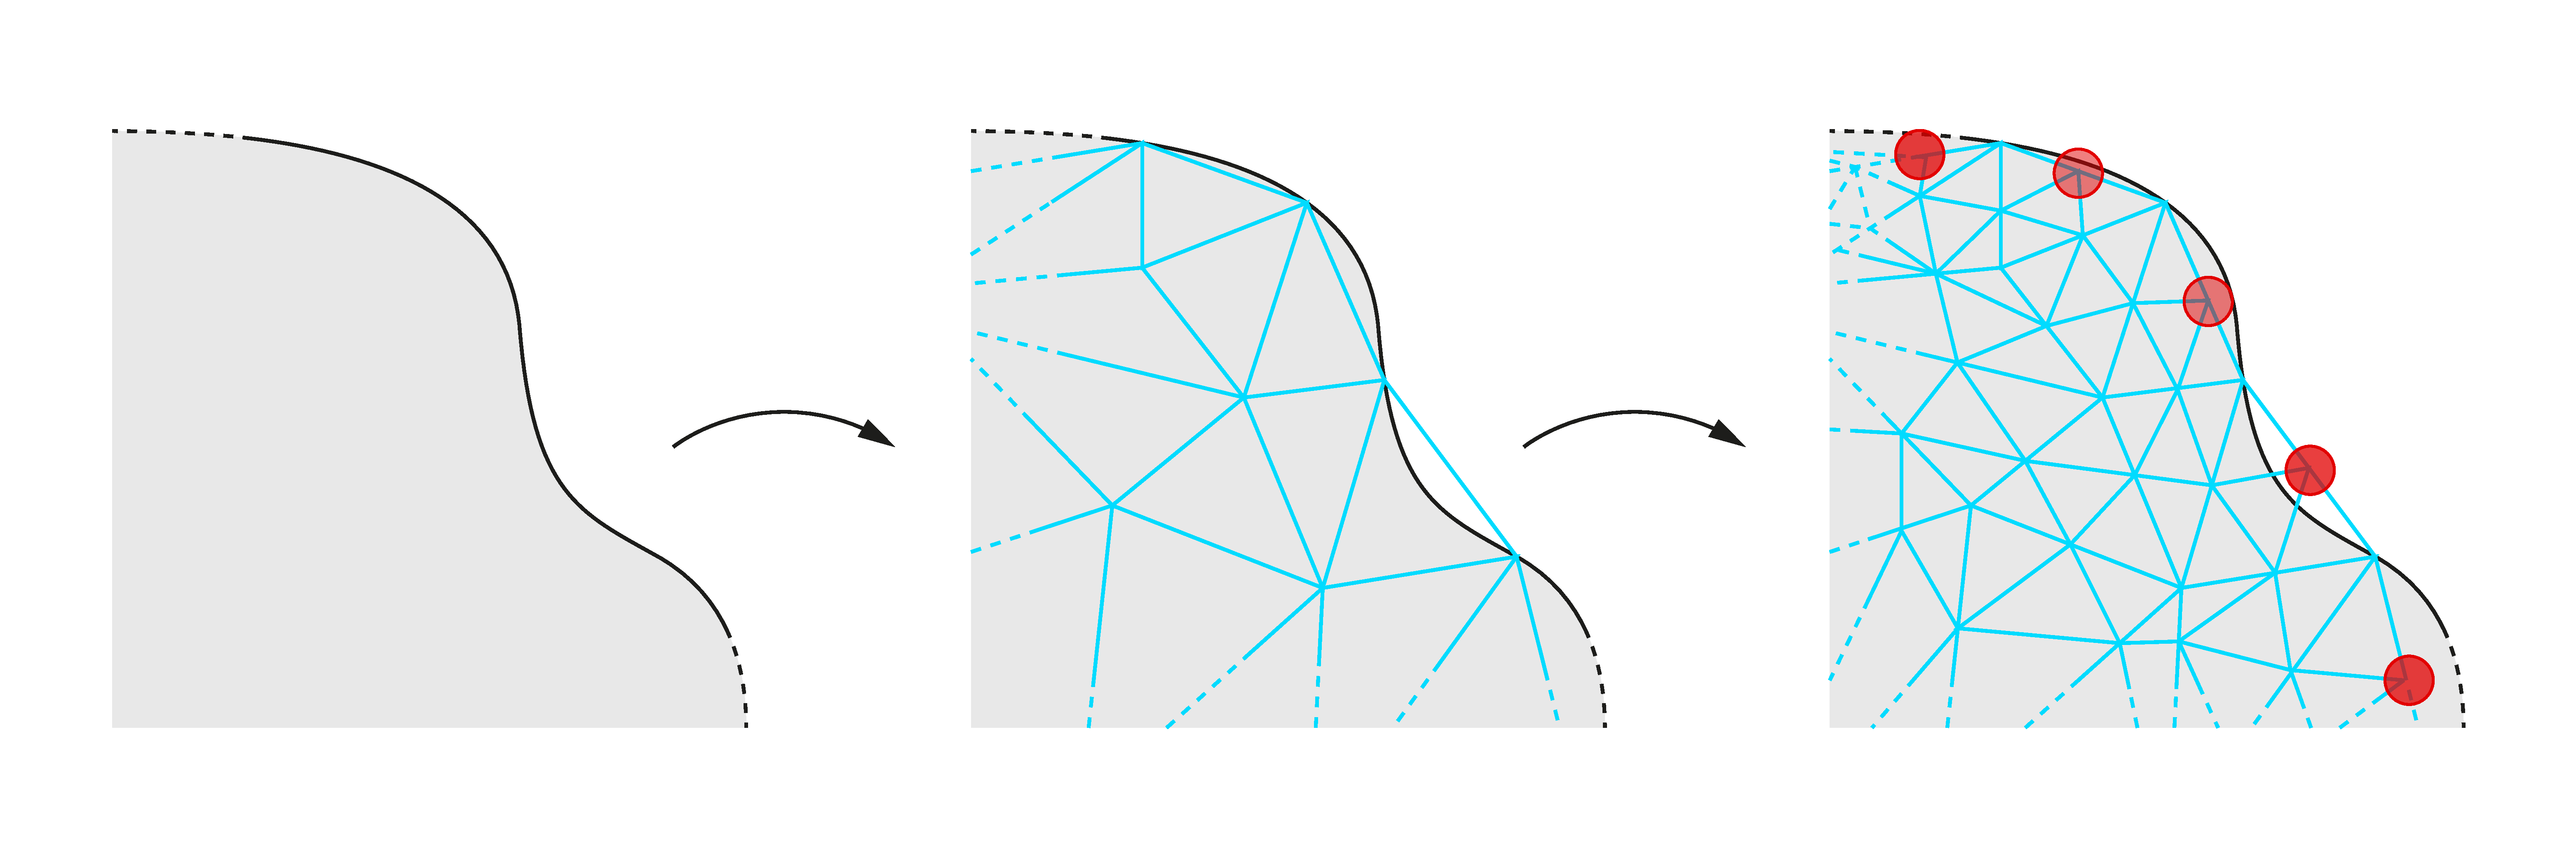
\includegraphics[width=0.95\columnwidth]{Images/UniformRefinement.pdf}
\caption{Problems with uniform refinements}\label{fig:uniform_refinement}
\end{figure}

\underline{Star-shaped parametrization}

For simplicity, we assume that the computational domain can only undergo radial displacements of the form given in \cref{cor:star_shaped_transformation}. This is realized as follows. The reference domain is fixed to be a meshing of $D\setminus \overline{B_\epsilon(0)}=:U_r$, meshing which induces the space of linear finite elements $S^1_h$, as we have denoted it in e.g. \cref{chap:inh_fem}. Consider also a meshing of the unit sphere $\mS$, potentially independent of the previous one to allow some flexibility, inducing the space of (surface) linear finite elements $B^1_{\tilde{h}}$. Our control, i.e. our optimization variable, will be a function $ \sigma_{\tilde{h}} \in B^1_{\tilde{h}}$, and we should be solving:

\begin{align*}
	\min_{\sigma_{\tilde{h}} \in B^1_{\tilde{h}}} J_{h,\delta t}(\tau_{\eps+\sigma_{\tilde{h}}}) = J_{h,\delta t }(\id  + V_{\sigma_{\tilde{h}}})
\end{align*}

with $V_{\sigma_{\tilde{h}}}$ being the vector field described in  \cref{cor:star_shaped_transformation}. The issue with this formulation is that  $V_{\sigma_{\tilde{h}}}$ doesn't preserve the polygonal/polyhedral nature of the volume meshes. Therefore, we actually implement:

\begin{align*}
	\min_{\sigma_{\tilde{h}} \in B^1_{\tilde{h}}}J_{h,\delta t }(\id  + I_h V_{\sigma_{\tilde{h}}})
\end{align*}

where $I_h$ means Lagrange interpolation onto piecewise linears.

We chose finite element functions on the sphere for simplicity. A downside that is more of theoretical nature, is that it is not clear to which smooth domain a deformed mesh corresponds to, because of the lack of smoothness of $B^1_{\tilde{h}}$ functions. One could then opt for smoother radial functions, like spherical harmonics, as it is done in \cite{harbrecht}. We did not follow this path for the sake of simplicity, as e.g. spherical harmonics or splines are not pre-built in FEniCS.

% The transformation $\sigma_{\tilde{h}} \mapsto I_h V_{\sigma_{\tilde{h}}}$ is implemented in a user defined dolfin-adjoint module.

\underline{Synthetic data}

As previously mentioned, to obtain the needed boundary data to perform shape optimization, we simulate the heat equation for $w$ on the exact computational domain $\Omega_{e,h}$. Because we are in a ``volumetric" setting, we give the Neumann data and obtain the Dirichlet nodal values, unlike in \cite{harbrecht}, where the opposite is done. In fact, in our setting, the finite element Neumann trace need not to have a boundary representation, so that the implementation becomes complicated.
%, plus, we found it more complicated from a code point of view, at least with the tools at our disposal, to deform the Neumann trace 

Using the same discretization parameters to generate the synthetic data, and then perform shape optimization, will result in committing an ``inverse crime" (see \cite{wirgin}). To avoid this, there are at least two possibilities: either some noise is added to the synthetic data, or different computational models must be employed in synthesis and inversion/optimization. We experiment with both options, and in particular, for the second, we synthethize the needed data with a finer discretization than during the optimization process. We mention that in \cite{harbrecht}, synthesis and inversion are performed by solving integral equations of different kinds, but on the same discretization. The authors also add noise to the synthetic data.  

\underline{Finite elements}

We are adopting, as already mentioned, linear (instead of e.g. quadratic) finite elements, for simplicity, but also computational efficiency. This is in constrast with \cite{harbrecht}, where the authors employ order $2$ isoparametric elements (in the context of the boundary element method). The framework of \cref{chap:inh_fem} could nonetheless potentially accommodate higher order isoparametric elements, see the works of e.g. \cite{edelmann}, \cite{elliott}, \cite{ranner}. Isoparametric elements are necessary, when adopting higher order basis functions, in order to preserve optimal accuracy (see section 4.4 of \cite{strang} for a discussion on this). The version of FEniCS we are using (2019.1) doesn't provide support for curved geometries, and the latest release FEniCSx is not yet interfaced with dolfin-adjoint. Alternatively, Firedrake (see \cite{firedrake}) could be employed, which has compatibility with dolfin-adjoint, although we encountered several difficulties in the transfering of functions between non conforming meshes, something we needed at several places throughout our code.

Also, we recall that the motivation for using the FEM method is that the analysis of \cite{paganini}, which we partially repeated in our setting, suggests that the volume form of the shape gradient is more accurate than a boundary form, when PDEs are discretized with the finite element method. Finite elements are also appreciated and widespread in the engineering community.
The main drawback of adopting a distributed setting is the added computational cost: the entire domain must be meshed, and the solution computed on interior nodes too.

\underline{Optimization}

As previously mentioned, we make use of the package Moola. This is because of its capabilities to natively handle optimization with respect to custom scalar products, and we found this to be especially important in our case, see \cref{sec:hilbert} for a theoretical justification and \cref{sec:experiments} for a further discussion.

We mostly experimented with an L-BFGS algorithm, but also with a modified Newton's method. We implemented the latter following the observations contained in \cite{eppler}, a work centered around a similar shape optimization problem as ours, in an attempt to alleviate some spurious oscillations we observed, most likely coming from the ill-posedness of the shape identification problem. We will soon discuss these aspects in \cref{sec:experiments}.

With regards to the temporal weight (see \cref{sec:o-t-d} for details), we chose $\eta(t) = \exp\{-a/(t-T)^2\}$, with a suitable $a>0$ ($a=0.005$ in our runs). $\eta$ roughly looks like this:

\begin{figure}[H]
\centering
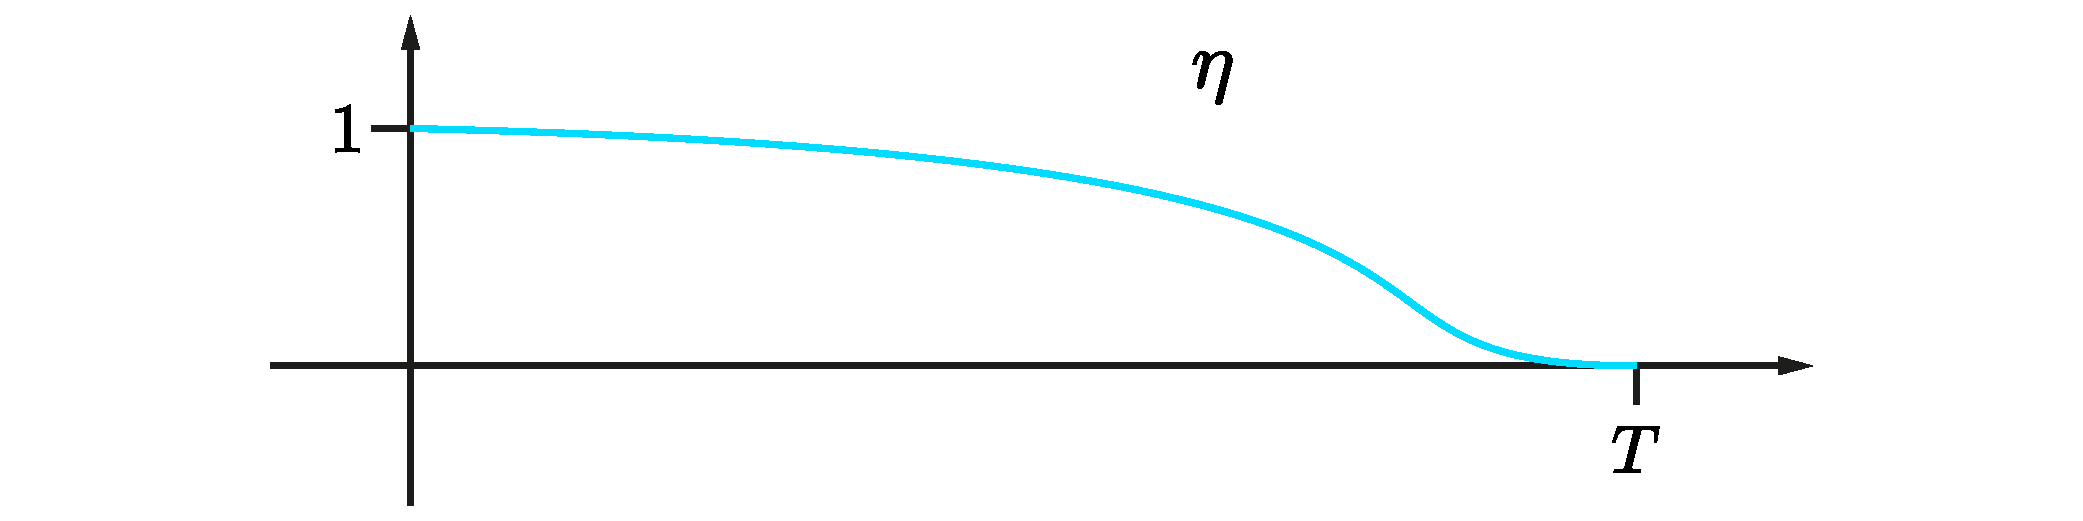
\includegraphics[width=0.6\columnwidth]{Images/Eta.pdf}
\caption{The temporal weight $\eta$}\label{fig:eta}
\end{figure}

\section{Experiments}
\label{sec:experiments}

All the experiments were conducted on a laptop with an Intel\textsuperscript{®} i7-6700HQ, 2.60GHz CPU, and 16 GB of RAM.

For simplicity we work in two dimensions and with $D:=B_2(0)$, $\Omega_r := B_{1}(0)$, so that $U_r$ is an annulus centered at the origin. 

\subsection{Shape optimization results}

We set $T=2$ throughout. Note that in the following plots, the ``exact" control (yielding the exact domain $\Omega_{e,h}$) is always interpolated into the finite element space of the control $\tilde{\sigma}_h$, to emphasize what is the best possible result that can be attained by the optimization routine.
%
%\begin{figure}[H]
%\centering
%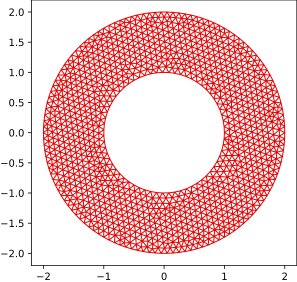
\includegraphics[width=0.3\columnwidth]{Images/hourglass_constant/initial_domain.pdf}
%\caption{Initial guess for the shape optimization process}\label{fig:initial_domain}
%\end{figure}

\underline{Some exploratory runs}

Let us illustrate a few runs, performed with different Neumann data $g$ and with an hourglass-shaped inclusion. The challenge of this example is to correctly resolve the ``corners" in the middle of the hourglass, which have a strong derivative (in the sense of radial functions), are far away from the external boundary (so that the influence on the boundary data of the heat equations may be weak), and where the mesh becomes very distorted, which worsens the quality of the mesh and thus, possibly, of the finite element solution.

To avoid the inverse crime, the Dirichlet data is generated on a mesh that is twice as fine as the to-be-optimized one, and with $120$ steps of the Crank-Nicolson method, whereas $60$ are used in the simulation. The sphere mesh size $\tilde{h}$ is set to $0.03$ during synthesis, and to $0.15$ during inversion. Such configuration will be referred to as ``standard configuration".

We show the results of six runs performed with six different Neumann sources: $g_1 = t^2$, $g_2 = x_1g_1$, $g_3=x_2g_2, g_4 = t^2\sin(4t), g_5 = t, g_6 = 1$. The examples took $25, 20, 20, 25, 25, 25$ L-BFGS iterations to converge, amounting to around $4$ minutes for each run.

$g_2, g_3, g_4$ represent various complications of the base example $g_1$, and we experiment with them to point out that there doesn't seem to appear a recurring ``error shape" when varying the boundary data $g$.

\begin{figure}[H]
\centering
\includegraphics[width=0.3\columnwidth]{Images/hourglass_oscillating/comparison.pdf}
\includegraphics[width=0.3\columnwidth]{Images/hourglass_linear/comparison.pdf}
\includegraphics[width=0.3\columnwidth]{Images/hourglass_quadratic/comparison.pdf}
\caption{Exact (in blue) and simulated inclusion (in red) for the runs with $g_2,g_3$ and $g_4$, in order from left to right}\label{fig:comparison_neumann}
\end{figure}

On the other hand, the heat equations with $g_5,g_6$ lack, respectively, one and two orders of compatibility, that are required in \cref{ass:num_discr_shopt}. We can see a better result in $g_1$, then in $g_5$ and lastly in $g_6$:

\begin{figure}[H]
\centering
\includegraphics[width=0.45\columnwidth]{Images/hourglass_constant_1_2_cropped.pdf}
\caption{From the outside to the inside: run with $g_6, g_5, g_1$ and exact solution in blue}\label{fig:comparison_compatibility}
\end{figure}


%For completeness, we report a picture of the final deformed mesh corresponding to the $g_1$ run:

%\begin{figure}[H]
%\centering
%\includegraphics[width=0.3\columnwidth]{Images/hourglass_constant/estimated_domain.pdf}
%\caption{Estimated domain in the $g_1$ run}\label{fig:estimated_domain}
%\end{figure}

For completeness, with $g_1$, we also report the history of the cost function and the gradient $l^\infty$ norm, after taking the logarithm:

\begin{figure}[H]
\centering
\includegraphics[height=0.25\columnwidth]{Images/hourglass_constant/comparison.pdf}
\includegraphics[height=0.25\columnwidth]{Images/hourglass_constant/cost_function.pdf}
\includegraphics[height=0.25\columnwidth]{Images/hourglass_constant/gradient_infty_norm.pdf}
\caption{Reconstruction, cost function (logarithm) and gradient history (logarithm) for the $g_1$ run and $25$ iterations}\label{fig:hourglass_constant}
\end{figure}

\underline{The effect of $\eta$}

We now show a visual comparison of the same example $g_1$, run with three different values $a$ for $\eta(t) = \exp\{-a/(t-T)^2\}$, which are $a=0.005, a = 0.05$ and $a=0$.

\begin{figure}[H]
\centering
\includegraphics[width=0.35\columnwidth]{Images/hourglass_constant_no_eta_more_eta_cropped.pdf}
\caption{From outside to inside: run with $g_1$ and $a=0$, $a = 0.05$, $a=0.005$ and exact solution in blue}\label{fig:eta_run}
\end{figure}

Some very small differences can be noticed: it seems that small values of $a$ yield an improvement over a $0$ value of $a$. Our hypothesis for this is in accordance with the behaviour of \cref{fig:comparison_compatibility}: $a=0$ means losing some compatibility, hence, possibly, accuracy. A too large value of $a$, on the other hand, perturbs the problem too much (so that the plot corresponding to $a=0.005$ yields the best result here). From here, we conjecture that $a$ should be chosen small enough, but positive.


\underline{Inner product}

We found it beneficial to work with smooth descent directions by making use of the $H^1$ inner product during optimization, instead of the $L^2$ one. This is natively handled by Moola. In doing so we obtained less squiggly boundaries, and more admissible ones: note in fact that we are working in an unconstrained setting for simplicity, whereas the optimization variable $\tilde{\sigma}_h$ should be positive and small enough for the computational domain to be contained in $B_{2}(0)$. With the $L^2$ scalar product we found that iterates were sometimes assuming negative values.

\begin{figure}[H]
\centering
\includegraphics[height=0.3\columnwidth]{Images/hourglass_constant_l2/comparison.pdf}
\caption{Reconstruction for the run $g_1$ and the $L^2$ inner product}\label{fig:l2}
\end{figure}


\underline{Ill-posedness}

\textit{Degeneration of the boundary}

It has already been noted in \cite{harbrecht} that \cref{pb:shid} is ``severely ill-posed". The ill-posedness of the inverse problem is mirrored in the ill-posedness of the shape optimization problem, \cref{pb:shopt}, where the responsible for such ill-posedness is the compactness of the continuous shape Hessian at the optimal domain: this phenomenon has been exhaustively analyzed in \cite{eppler} in an ``elliptic" version of \cref{pb:shid}, but we expect similar conclusions to apply also to our case.

We computed the shape Hessian at the optimal domain with the help of dolfin-adjoint and observed indeed large condition numbers, as expected (with values $\simeq 10^5$).

This means that small changes in the problem data might yield large changes in the reconstruction, and instabilities in the reconstruction process. In fact, as is commonplace in solving ill-posed inverse problems, proceeding further with the iterations of the solution algorithm will only at first improve the reconstruction, but later result in a degradation (see e.g. \cite{kirsch}, section 2.1). As a remedy, one should impose prior knowledge on the reconstruction through regularization, and/or adopt some form of early stopping. 

We did experience these phenomena: up to a certain number of L-BFGS iterations, we obtained acceptable results, the ones we showed above. Proceeding further led to a degradation of the inner boundary. To counter this, we adopted early stopping. A smoothing effect is already provided by the choice of the inner product, and we did not find additional benefits from implementing a Tikhonov regularization. Now, the run with $g_1$ and stopping at $75$ iterations instead of $25$, produced:

\begin{figure}[H]
\centering
\includegraphics[height=0.25\columnwidth]{Images/hourglass_constant_degenerate/comparison.pdf}
\includegraphics[height=0.25\columnwidth]{Images/hourglass_constant_degenerate/cost_function.pdf}
\includegraphics[height=0.25\columnwidth]{Images/hourglass_constant_degenerate/gradient_infty_norm.pdf}
\caption{Reconstruction, cost function (logarithm) and gradient history (logarithm) for the $g_1$ run and $75$ iterations}\label{fig:degenerate}
\end{figure}

The solution obtained at around $25$ iterations remains unchanged and stable until about iteration $35$, then the cost function is further reduced, along some spurious descent direction. Note the oscillatory behaviour of the gradient norm.

This degeneration is even more evident and quicker, in case the implicit Euler method is used during optimization, in place of the Crank-Nicolson one, leaving all the other parameters unchanged (so that the exact data is still generated with the Crank-Nicolson method). This is because the implicit Euler method converges more slowly in time, so that the discrepancy in the computed PDEs and the synthetic PDEs, is $O(\delta t)$ and not $O(\delta t^2)$. This is one of the reasons for adopting the Crank-Nicolson method: the implicit Euler method yields a faster, worse degeneration of the boundary, and a less accurate one, when early stopping is applied. We have nonetheless analyzed the implicit Euler case in \cref{chap:discretization} because this method has already been successfully employed in less ill-posed parabolic shape optimization (see \cite{lindemann2}). We show reconstruction, cost function and gradient history for a run with implicit Euler.

\begin{figure}[H]
\centering
\includegraphics[height=0.25\columnwidth]{Images/comparison_25_45_euler.pdf}
\includegraphics[height=0.25\columnwidth]{Images/hourglass_constant_euler/cost_function_45.pdf}
\includegraphics[height=0.25\columnwidth]{Images/hourglass_constant_euler/gradient_infty_norm_45.pdf}
\caption{Reconstruction, cost function (logarithm) and gradient history (logarithm) for the $g_1$ run. The black boundary corresponds to $45$ iterations, the blue one to $25$. The presence of the lateral lobes in the black reconstruction indicates a negative radial function.}\label{fig:degenerate_euler}
\end{figure}

\textit{About the inverse crime}

Let us avoid the inverse crime in a different way, through application of noise to the problem data $f,g$. We therefore set the discretization parameters for the synthetization to be equal to those used for the inversion. The noise level is $1$\%, with respect to the $L^\infty(I,L^\infty)$ norm of the data, and the perturbation is random uniform. 

We noticed that the optimization process is much more stable with the number of iterations, than when different discretizations are adopted, for inversion and synthesis. The reconstructed boundary is very similar to those of the above runs, and it starts to present spurious oscillations  very late (only after iteration $80$, in the case of the $g_1$ run). The discrepancy between exact data and data available during optimization, is randomly distributed and of zero mean, whereas we noted that it presents a ``trend" given by the chosen PDEs discretization algorithm, when different discretizations are employed. This seems to be a key ingredient for the degeneration behaviour that we observed. 

We did most of the experiments with different discretizations between inversion and synthesis, because this approach better highlited the ill-posedness of the problem. Moreover, in a real-world situation, the actual boundary data can be interpreted to be sampled from a solution with discretization parameters tending to zero: this is another reason to proceed as we did.

\textit{Second order information}

As previously mentioned, there is some evidence to conclude that the shape optimization problem is ill-posed: this is reflected in an ill-conditioned Hessian, at the optimal domain. This can cause undesired oscillations when employing only first order optimization methods, a possible way out being the usage of additional second order information, like the shape Hessian.

We thus experimented with a regularized Newton method, following the observations of \cite{eppler} (to which we refer the reader for further details about the method), and found out that, indeed, spurious oscillations don't seem to happen: using $g_1$ as Neumann data, we find that it takes about $20$ iterations for the shape to stabilize. However, the runtime increases to about $2.75$ minutes per iteration, the shape Hessian being automatically computed by dolfin-adjoint. On top of this, the reconstruction seems to be less precise than when employing the L-BFGS method, with early stopping. This convinced us to stick with the L-BFGS method. 

\begin{figure}[H]
\centering
\includegraphics[height=0.25\columnwidth]{Images/hourglass_constant_newton/comparison.pdf}
\includegraphics[height=0.25\columnwidth]{Images/hourglass_constant_newton/cost_function.pdf}
\includegraphics[height=0.25\columnwidth]{Images/hourglass_constant_newton/gradient_infty_norm.pdf}
\caption{Reconstruction, cost function (logarithm) and gradient history (logarithm) for the $g_1$ run, and the regularized Newton method from \cite{eppler}. The reconstructions after $20$ and $70$ shape are visually indistinguishable.}\label{fig:newton}
\end{figure}

\underline{More complicated examples}

Lastly, we show the reconstructions for two more complicated exampls. In both cases, the discretization configuration is the standard one, and for completeness, we applied also $1$\% noise to the data, apart from employing different discretizations in inversion and synthesis.

We start with a 2D version of the ``sea urchin" inclusion from \cite{harbrecht}, and let the simulation run for $30$ iterations. 

\begin{figure}[H]
\centering
\includegraphics[height=0.3\columnwidth]{Images/sea_urchin/exact_domain.pdf}
\includegraphics[height=0.3\columnwidth]{Images/sea_urchin/estimated_domain.pdf}
\includegraphics[height=0.3\columnwidth]{Images/sea_urchin/comparison.pdf}
\caption{``Exact" domain, reconstruction, and comparison between reconstruction and the exact domain, interpolated to the optimization finite element space.}\label{fig:sea_urchin}
\end{figure}

Instead of the cat-shaped inclusion from \cite{harbrecht}, which is not very well suited for a star-shaped parametrization, we experiment at last with a duck-shaped one, also in two dimensions. This time, the exact domain is non convex and presents sharp corners, so that $H^2$ regularity won't hold and the finite element solutions will not be display optimal order convergence. Nonetheless, this is the result after $90$ iterations:

\begin{figure}[H]
\centering
\includegraphics[height=0.3\columnwidth]{Images/duck/exact_domain.pdf}
\includegraphics[height=0.3\columnwidth]{Images/duck/estimated_domain.pdf}
\includegraphics[height=0.3\columnwidth]{Images/duck/comparison.pdf}
\caption{``Exact" domain, reconstruction, and comparison between reconstruction and the exact domain, interpolated to the optimization finite element space.}\label{fig:duck}
\end{figure}

%\tred{hessian in L-BFGS}

\subsection{Estimates for the shape gradients}

We now present some numerical evidence of the estimates shown in \cref{sec:d-t-o_IE}. Throughout, $U_h$ will be approximating $U = B_2(0)\setminus \overline{B_1(0)}$, we set $\delta t = 5 h^{2\theta}$ (where $\theta=1$ for implicit Euler or $\theta=1/2$ for Crank-Nicolson) and $a = 0.005$ (this is the parameter to control the steepness of the temporal weight $\eta$).

We choose a number of spikes $s$ from $0$ to $9$, an amplitude among $0.1$ and $0.2$ and we consider the resulting sinusoidal radial function $\sigma(t) = A \cos(st)$, interpolated on a spherical mesh of size $\tilde{h} = 0.5$. This mesh parameter stays fixed across all the runs, when $h$ varies. Note, this yields a very coarse spherical mesh: the rationale is to have the resulting displacement fields $V_\sigma$ (see \cref{sec:star}) approximating a vector field that is in $W^{1,\infty}$ but not $W^{2,\infty}$, as $h$ is refined. We thus obtain  $20$ different displacement fields $\delta \te_{h,\tilde{h}}^i$, $i=1,...,20$, with which we test the shape gradients.  We additionally consider $10$ more vector fields that are non-radial and $C^\infty$, whose components are degree $3$ polynomials (similarly to \cite{paganini}). 


Not being able to represent non-discretized shape gradients, we content ourselves with analyzing the asymptotic behaviour of the quantity:

$$Q_h:=\max_{i=1,...,30}\frac{|J'_{h_f,\delta t_f}(U_{h_f})[\delta \te_{h_f,\tilde{h}}^i]-J'_{h,\delta t}(U_h)[\delta \te_{h,\tilde{h}}^i]|}{\norm{\delta \te_{h,\tilde{h}}^i}_{W^{1,\infty}(U_{h_f})}}$$

where $h_f \ll h$, $\delta t_f \ll \delta t$.

In particular, we set $h_f = 0.015625$, and $h = 2^{l} h_f$, for $l$ integer, where we refer to $2^l$ as ``multiplier". We report the orders of convergence $\ds OOC =  \frac{\log Q_h-\log Q_{2h}}{\log h - \log 2h}$ in three cases:

%We set $C=1$ (for $\delta t = C h^{2\theta}$) for Crank-Nicolson, and $C=5$ for implicit Euler, to have a number of timesteps that is always greater than $1$. For reasons of computational resources, we made one less refinement in the implicit Euler case.
%
%\begin{table}[h]
%\centering
%\begin{tabular}{lllllll}
%\hline
%\textit{Multiplier} & $32$ & $16$ & $8$ & $4$ & $2$ & $1$\\ \hline
%$Q_h$ & $0.0557$ & $0.0139$ & $0.0047$ & $0.0013$ & $0.0003$ & $0.0$\\ \hline
%\textit{OOC} & $2.356$ & $1.8261$ & $2.0785$ & $2.4573$ & $\infty$ & $-$ \\ \hline
%\end{tabular}
%\caption{Run with Crank-Nicolson, $a = 0.05$ and $C = 1$}\label{tab:CN_eta_rough}
%\end{table}

\begin{table}[h]
\centering
\begin{tabular}{llllllll}
\hline
\multicolumn{8}{l}{\textbf{Crank-Nicolson, discretize-then-optimize}} \\ \hline
\textit{Multiplier} & $64$ & $32$ & $16$ & $8$ & $4$ & $2$ & $1$\\ \hline
%$Q_h$ &  $0.075$ & $0.019$ & $0.005$ & $0.001$ & $0.000$ & $6.377$ & $0.0$\\ \hline
\textit{OOC} & $2.314$ & $2.196$ & $2.252$ & $2.270$ & $2.153$ & $\infty$ & $-$ \\ \hline
\multicolumn{8}{l}{\textbf{Crank-Nicolson, optimize-then-discretize}} \\ \hline
\textit{Multiplier} & $64$ & $32$ & $16$ & $8$ & $4$ & $2$ & $1$\\ \hline
%$Q_h$ &  $0.075$ & $0.019$ & $0.005$ & $0.001$ & $0.000$ & $6.377$ & $0.0$\\ \hline
\textit{OOC} & $1.713$ & $1.831$ & $1.991$ & $2.061$ & $2.264$ & $\infty$ & $-$ \\ \hline
\end{tabular}
\caption{Order of convergence study with Crank-Nicolson}\label{tab:ooc_CN}
\end{table}


\begin{table}[h]
\centering
\begin{tabular}{lllllll}
\hline
\multicolumn{6}{l}{\textbf{Implicit Euler, discretize-then-optimize (commutative)}} \\ \hline
\textit{Multiplier} & $64$ & $32$ & $16$ & $8$ & $4$\\ \hline
%$Q_h$ & $0.0549$ & $0.0154$ & $0.0047$ & $0.001$ & $0.0$\\ \hline
\textit{OOC} & $2.120$ & $1.963$ & $2.300$ & $\infty$ & $-$ \\ \hline
%\hline
%\multicolumn{6}{l}{Run with implicit Euler, $a = 0$ and $C=5$} \\ \hline
%\textit{Multiplier} & $16$ & $8$ & $4$ & $2$ & $1$\\ \hline
%$Q_h$ & $0.0594$ & $0.0126$ & $0.005$ & $0.0011$ & $0.0$\\ \hline
%\textit{OOC} & $2.5864$ & $1.5225$ & $2.2349$ & $\infty$ & $-$ \\ \hline
\end{tabular}
\caption{Order of convergence study with implicit Euler: the last two refinement are not done, due to issues of computing power}\label{tab:ooc_IE}
\end{table}

Of course we register an infinite order of convergence when the refinement brings us from $2h_f$ to $h_f$. Moreover, the order of convergence value in the second-last refinement is always larger than expected, most probably because of a ``saturation" effect. We think that these results confirm the theoretical considerations of \cref{sec:d-t-o_IE}. In particular, we note the following facts:

\begin{itemize}
	\item \cref{tab:ooc_IE}, \cref{tab:ooc_CN} suggest an $O(h^2+\delta t^\te)$ order of convergence, even with ``rough" vector fields, cfr. \cref{cor:superconvergence_sd_fd_IE} and \cref{cor:superconvergence_sd_fd_CN}. With rough vector fields, we remind that we could theoretically only obtain $O(h+\delta t^\te)$ convergence, see also \cite{paganini}
	\item although we haven't given a proof of the convergence behaviour in the case of the Crank-Nicolson method and a discretize-then-optimize approach, the table suggests that the quantity $Q_h$ is $O(h^2+\delta t^2)$, as we suspected. Note, spatial superconvergence effect happens also here, although $W^{1,\infty}$ displacements are included 
%	\item the value of $1.5225$ in \cref{tab:ooc_CN} might be due to a lack of regularity of the adjoint states, since $a=0$. This does not contradict our predictions, which were done in conditions of $a>0$
\end{itemize}

\chapter{Conclusion}
\label{chap:conclusion}

We considered a model parabolic shape optimization problem and treated it in a volumetric fashion: the expression of the distributed shape gradient was derived, also in connection to a star-shaped parametrization of the domains.

The finite element method was employed to perform the spatial discretization of the arising PDEs, whereas a Crank-Nicolson or implicit Euler scheme was adopted for the temporal one. In the latter case, optimization and discretization are seen to commute.

We derived a semidiscrete (in space) error estimate relating the continuous shape gradient at a smooth enough domain $U$, and the discrete shape gradient at a polygonal/polyhedral interpolation $U_h$ of $U$. In the case of the implicit Euler method, we were able to obtain from that, fully discrete estimates in a discretize-then-optimize commutative setting, whereas for the Crank-Nicolson one, only in an optimize-then-discretize framework.

Numerical experiments support such conclusions, and even suggest that what was only proved for the implicit Euler method, might be obtainable with the Crank-Nicolson method. We also show results of the shape optimization process itself.

There are some interesting directions in which our work can be expanded:

\begin{itemize}
	\item one could at first prove that discretization and optimization commute also for Crank-Nicolson, see e.g. \cite{flaig} for a promising starting direction (which needs however adaptations to accommodate our analysis of smooth geometries). From here, fully discrete estimates analogous to those for implicit Euler, should be obtainable
	\item the error estimates for the shape gradients were derived assuming a specific form of $U_h$: it could be worth to try to eliminate the requirement that $\partial U_h$ must interpolate $\partial U$, or to devise a finite dimensional domain parametrization that is e.g. $C^2$, so that is is clear which domain $U_h$ is interpolating, during shape optimization. Moreover, one could try to explicitly account for the fact that $U=\tau (U_r), U_h = \tau_h(U_{r,h})$, in these estimates, i.e. making the contribution of $\tau, \tau_h$ explicit
	\item experimenting with higher order finite elements, both theoretically and in the implementation, should yield better error estimates for the shape gradients and, potentially, better shape optimization results. The framework of \cref{chap:inh_fem} naturally extends in this direction, see e.g. \cite{ranner}, \cite{elliott}
	\item one could repeat the analysis with time-dependent domains, \cite{ranner} provides a good foundation for this, too, at least for the finite element discretization
	\item finally, one could experiment with schemes that don't require so much regularity in time, so as to eliminate the need for the temporal weight $\eta$
\end{itemize}

%
%\renewcommand{\appendixname}{Appendice}
%\renewcommand{\appendixpagename}{Appendici}
%\renewcommand{\appendixtocname}{Appendici}
\renewcommand\chaptername{Appendix}
\begin{appendices}

\appendix
\makeatletter
\renewcommand*{\chapterformat}{%
  \mbox{\chapapp~\thechapter\autodot\enskip}%
}
\makeatother



\chapter{Functional spaces}
\label{chap:functional_spaces}
Let us collect, for the convenience of the reader, some technical results that will be used throughout our work. Where appropriate, we give a short proof or a reference for one.

\section{Sobolev spaces}

\begin{thm}[Integration by parts]
\label{thm:ibp}
Let $\Omega$ be a bounded Lipschitz domain. Let $1<p<\infty$ and $f,g \in W^{1,p}(\Omega), W^{1,q}(\Omega)$, $q=p'$, the dual Hölder exponent. Then:

$$\int_\Omega f \partial_i g = -\int_\Omega g \partial_i f+\int_{\partial \Omega} \tr u \nu_i d\pazocal{H}^{n-1}$$
\end{thm}
\begin{mproof}

This follows from \cite{leoni}, theorem 18.1 at page 592, where $g$ needs to be $C^1_c(\mR^n)$. But from \cite{adams}, theorem 3.18 at page 54, thanks to the smoothness of the boundary, the set of the restrictions to $\Omega$ of such functions is dense in $W^{1,q}(\Omega)$, so that we can conclude by a density argument.
\end{mproof}

%\begin{lemma}
%$f \in L^\infty(\Omega; \mR^N) \iff f_i \in L^\infty$, and two equivalent norms are $\norm{f}_a:=\norm{|f|}_\infty$, $\norm{f}_b:=\max_i\norm{f_i}_\infty$, for $|\cdot |$ any finite dimensional norm.
%\end{lemma}
%\begin{mproof}
%
%We choose $|\cdot |=|\cdot|_1$.
%
%Consider $f_n \in X_a = \{[f], f: \Omega \rightarrow \mR^n \text{ measurable }, \norm{f}_a\}$, Cauchy. Then every component is Cauchy in the scalar $L^\infty$, so that $f_n^i \rightarrow f^i $ in $L^\infty$. The limit $f$ is in $X_a$ because the functions $|f_i|$ are essentially bounded, and so is $|f|$. 
%
%Then $\norm{f_n-f}_a\leq \norm{f_n-f_m}_a+\sum_i\norm{f_m^i-f^i}_\infty$ for all $n,m$. Choose $m\geq n$ with $\norm{f_m^i-f^i}\leq 1/(Nn)$ and conclude $X_a$ is Banach.
%
%We know from \cite{leoni}, theorem B.88 at page 671, and page 669, we know that $X_b = \{[f], f: \Omega \rightarrow \mR^n \text{ measurable }, \norm{f}_b\}$ is Banach.
%
%Moreover $X_a=X_b$ as sets, so that the thesis follows.
%
%
%%We have that $\norm{f}_\infty = \sup_{\Omega\setminus X}f$ for all $X$ null sets on which $f \leq \norm{f}_\infty$ on $\Omega \setminus X$.
%%
%%In fact, that  $\norm{f}_\infty \geq \sup_{\Omega\setminus X}f$ is clear, whereas suppose there is $\epsilon >0$ with $\norm{f}_\infty -\epsilon \geq f$ on $\Omega \setminus X$. Then we contradict the definition of essential supremum and therefore $\norm{f}_\infty = \sup_{\Omega\setminus X}f$.
%%
%%Next up: for some $X,Y \subseteq \Omega$ of measure $0$, $f,g\leq \norm{f}_\infty, \norm{g}_\infty$ in $\Omega\setminus X, \Omega \setminus Y$, therefore, for some $N$ of null measure, $f,g\leq \norm{f}_\infty, \norm{g}_\infty$ in $\Omega \setminus N$. Therefore, $\norm{f}_\infty = \sup_{\Omega \setminus N}f, \norm{g}_\infty = \sup_{\Omega \setminus N}g$. 
%%
%%Therefore $ \max(\norm{f}_\infty, \norm{g}_\infty) = \max(\sup_{\Omega \setminus N}f,  \sup_{\Omega \setminus N}g) = \sup_{\Omega\setminus N}\max(f,g)$.
%%
%%So, $N$ is a null set and $\max(f,g)\leq \max(\norm{f}_\infty, \norm{g}_\infty)$, which by the reasoning of before.
%%
%%
%
%\end{mproof}

\begin{prop}[Characterization of $W^{1,\infty}$]
\label{prop:lip}
Let $\Omega$ be a bounded Lipschitz domain, or $\mathbb{R}^n$. Then $W^{1,\infty}(\Omega) = C^{0,1}(\overline{\Omega})\cap L^\infty(\Omega)$.

This means that $u\in W^{1,\infty}(\Omega)$ if and only if $u$ has a (unique) representative that is bounded, Lipschitz continuous. Weak and classical derivatives coincide a.e.
\end{prop}
\begin{mproof}

%\underline{ACL characterization}
%
%Let $\Omega$ be just a domain.
%
%Consider a line $\gamma$ intersecting $\Omega$. Then, the intersection is a disjoint union of open segments $\gamma_i$. We say $u\in AC_\gamma(\Omega)$ if and only if $u$ is $AC[a,b]$ for every $[a,b]\cc\eta_i$ for all $i$, for almost all lines $\eta$ parallel to $\gamma$ and intersecting $\Omega$.
%
%We say $u \in ACL(\Omega)$ if $u$ is $AC_{e_i}(\Omega)$ for all coordinate axis $e_i$. We also call $BL(\Omega)$ the set of $u$ with a representative $\tilde{u}$, with $\tilde{u}\in ACL(\Omega), \tilde{u}, \nabla \tilde{u} \in L^\infty$, $\nabla u$ being the classical (a.e.) gradient.
%
%We have the following result (see \cite{kufner}, page 276, theorem 5.6.5.): $u \in W^{1,\infty}(\Omega)$ if and only if $u$ has a representative $\tilde{u} \in BL(\Omega)$. Classical and weak derivatives then coincide a.e..

In any case, $\Omega$ is an extension domain for $W^{1,\infty}(\Omega)$ (see \cite{leoni}, theorem 13.17 at page 425, 13.13 at page 424, and definition 9.57 at page 273).

Let $u \in  W^{1,\infty}(\Omega)$. By \cite{leoni}, 11.50 at page 339, because $\Omega$ is an extension domain, we obtain that $u$ has a representative $\bar{u}$ that is bounded Lipschitz. Let $\phi \in C_c^\infty(\Omega)$. By The Kirszbraun theorem (see e.g. \cite{kirszbraun}), we can extend $\bar{u}$ to a Lipschitz on $\mathbb{R}^n$. Then, by Fubini's theorem and integration by parts for $AC$ functions, we conclude $\ds \int_\Omega\bar{u}\partial_i\phi =-\int_{\Omega} \partial_i \bar{u} \phi $, so that $\nabla \bar{u} = \nabla u$ almost everywhere.

Conversely, let $u$ be bounded Lipschitz. The above reasoning shows that $u$ has (bounded) weak derivatives equal to the a.e. classical derivatives. Their measurability follows by approximation by difference quotients.
\end{mproof}

%Therefore, for $\phi \in C_c^\infty(\Omega)$ we get $\ds -\int_\Omega u \phi_{,i}\ds = \int_\Omega \partial_i u\phi =  \int_\Omega g_i \phi$.
%
%Pick a cube $Q = [-M,M]^n$, $\Omega \cc Q$. So, upon extending in a bounded Lipschitz manner $g_i$ to $G_i$ with $G_i(\partial Q)=0$ (see \cite{kirszbraun} and multiply by a suitable cut-off function), and $\phi$ to $0$, we get $\ds ...=\int_\Omega G_i \phi$. Call $h_i^x(t)=G_i(...,x_{i-1},t,x_{i+1},...)$ which is $AC[-M,M]$. Because $\eta_i^x(s):= \int_{-M}^s h_i^x(z)dz$ is $AC[-M,M]$ too because $h_i^x$ is bounded, and $h_i^x(t) =  \eta_i^{x'}(t)$. Employing then Fubini:
%
%\begin{align*}
%...= \int_{-M}^M... \int_{-M}^M \int_{-M}^M G_i(...,x_{i-1},x_i,x_{i+1},...)\phi dx_i dx_1...dx_{i-1}dx_{i+1}...dx_n  \\
%= \int_{-M}^M... \int_{-M}^M \int_{-M}^M h_i^x(x_i) \phi dx_i dx_1...dx_{i-1}dx_{i+1}...dx_n \\
%= \int_{-M}^M... \int_{-M}^M \int_{-M}^M \eta_i^{x'}(x_i)  \phi dx_i dx_1...dx_{i-1}dx_{i+1}...dx_n \\
%= \int_{-M}^M... \int_{-M}^M \int_{-M}^M \eta_i^{x'}(x_i)  \phi dx_i dx_1...dx_{i-1}dx_{i+1}...dx_n \\
%= -\int_{-M}^M... \int_{-M}^M \int_{-M}^M \eta_i^x(x_i)  \phi_{,i} dx_i dx_1...dx_{i-1}dx_{i+1}...dx_n \\
%=- \int_{-M}^M... \int_{-M}^M \int_{-M}^M \int_{-M}^{x_i} G_i(...,x_{i-1},z,x_{i+1},...) dz\phi_{,i} dx_i dx_1...dx_{i-1}dx_{i+1}...dx_n \\
%= -\int_Q k_i\phi_{,i}
%\end{align*}
%
%where in the last passage we have used again Fubini and the fact that 
%
%$$k_i(x):=\int_{-M}^{x_i} G_i(...,x_{i-1},z,x_{i+1},...) dz$$
%
% is measurable and bounded on $Q$.


\section{Bochner spaces}

%Here are some useful results about Bochner spaces.

\begin{prop}[Bochner integral and bounded operators]
\label{lemma:bochner_Hk_map}
%\label{prop:bochner_bound}
Let $X,Y$ be separable Banach, let $T \in L(X,Y)$ be a linear bounded operator. For $f \in L^1(I,X)$ define $Tf (t):= T(f(t))$. Then $Tf \in L^1(I,Y)$ with $\ds T\int_I f = \int_I Tf$.

More generally, for $k\geq 0$, $1\leq p < \infty$, $f \in W^{k,p}(I,X)\implies Tf \in W^{k,p}(I,Y)$, with weak derivatives $\partial_{t^i}Tf = T\partial_{t^i}f$, $0\leq i \leq k$.

The map $f \mapsto Tf$, $W^{k,p}(I,X)\rightarrow W^{k,p}(I,Y)$ is linear, and bounded by $\norm{T}$.

\end{prop}
\begin{mproof}

Let $f_n$ be simple, $f_n\rightarrow f $ a.e., with $\lim_n \int_I f_n = \int_I f$ in $X$ and $\norm{f_n}_X \leq C \norm{f}_X$ (see page 6, and corollary 2.7 at page 8 of \cite{kreuter}).

For almost all $t$, $T(f_n(t)) \rightarrow T(f(t))=Tf(t)$ in $Y$, so that $Tf$ is measurable (strongly).

By dominated convergence (corollary 2.6 of \cite{kreuter}), $Tf$ is integrable. Thus $\int_T Tf = \lim_n \int_I  Tf_n = \lim_n T\int_I  f_n$, because $f_n$ is simple. And now, by the choice of $f_n$, $\int_T Tf = \lim_n T\int_I  f_n = T \lim_n \int_I  f_n = T \int_I f$.

The rest of the claim is a straightforward consequence of this first part.
\end{mproof}

%\begin{cor}	[Derivations and bounded operators]
%\label{lemma:bochner_Hk_map}
%As before, let $X,Y$ be separable Banach, let $T \in L(X,T)$ be a linear bounded operator.
%
%\end{cor}
%\begin{mproof}
%The case $k=0$ is proved above.
%
%We prove now that $\partial_{t^i}Tf = T\partial_{t^i}f$ for $i=1$. Note that $T\partial_t f \in L^2(I,Y)$, which qualifies as weak derivative.
%
%In fact, for $\phi \in C_c^\infty(I)$, we have $\int_I \phi T\partial_i f = \int_I T(\phi\partial_t f) = T \int_I\phi\partial_t f = -T\int_I\phi'f=-\int_I\phi'Tf$.
%
%Higher weak derivatives are treated analogously and the rest of the claims follow from the time stationarity of $T$ and by $\norm{\partial_{t^i}Tf}=\norm{T\partial_{t^i}f}\leq \norm{T}\norm{\partial_{t^i}f}$.
%
%\end{mproof}

\begin{prop}[Continuous representatives]
\label{prop:cts_repr}
Let $X$ be separable Banach. $f \in L^1(I,X)$ has at most a continuous representative on $[0,T]$.
\end{prop}
%\begin{mproof}
%Assume there exists two such continuous representatives, so that we get a function $\delta: [0,T] \rightarrow X$ that is zero almost everywhere and continuous. Hence, $[0,T] \ni t \mapsto \norm{\delta(t)}$ is continuous in $\mR$ and zero a.e., so that it must be zero everywhere.
%\end{mproof}

%\begin{prop}[Weak derivatives and Gelfand triples]
%\label{prop:sob_implies_W}
%Let $H\subseteq V$ be separable Hilbert spaces, $H$ densely embedded in $V$.
%
%Then $y \in L^2(I,V)\cap H^1(I,H) \subseteq W(I,V)$.
%\end{prop}
%\begin{mproof}
%We note that $V$ is Hilbert separable, so, reflexive Banach and separable, so that $V^*$ is separable too. Then, call $i$ the embedding $H \emb V^*$.
%
%For $\phi \in C^\infty_c(I)$ we obtain $\int_I i(y_t)\phi=\int_I i(y_t\phi)= i \left ( \int_I y_t\phi \right )$ by \cref{lemma:bochner_Hk_map}. Therefore $\int_I i(y_t)\phi=-i \left ( \int_I y\phi' \right ) =\int_I i(y)\phi'  $ , proving that $y \in W(I,V)$.
%
%\end{mproof}

%We now check that a vector valued test function has weak derivatives of all orders.

\begin{prop}[Weak derivatives of test functions]
\label{prop:weak_class}
Let $\phi \in C^1([0,T],X)$, for $X$ separable Banach. It means that the limit of the difference quotients exists for all points of $I$, that $t\mapsto \phi(t), \phi'(t)$ are continuous, and that they can be continuously extended to $[0,T]$.

Then these classical derivatives coincide a.e. with the weak derivatives of $u$.

\end{prop}
\begin{mproof}


Apply proposition 3.8 of \cite{kreuter} at page 26, thanks to theorem 6 at page 146 of \cite{mvt}, a mean value theorem for vector valued function.
\end{mproof}

We also need a time dependent trace lemma, which we provide in a space-time ``tensor product" form, but under non-optimal regularity assumptions, for the sake of making some arguments more transparent.

\begin{prop}[Time dependent trace]
\label{prop:trace}
Let $\Omega$ be a bounded Lipschitz domain (in the sense of \cite{grisvard}, definition 1.2.1.1). For $k\geq 0$ we define $\tr_k: H^k(I,H^1(\Omega))\rightarrow H^k(I, H^{1/2} (\partial \Omega))$ by $\tr_k(u)(t):=\tr(u(t))$. The trace operator just defined:
\begin{enumerate}
\item is well posed, linear and bounded
\item admits a linear bounded right inverse, for instance, $E_k(g)(t):=E(g(t))$ (for $E$ a right inverse of the ``static" trace)
\item $\tr_k u = \tr_0 u$, for $u \in L^2(I,H^1(\Omega))$ and $E_k g = E_0g$ gor $g \in L^2(I,H^{1/2}(\partial \Omega))$, and we can thus drop the subscript $k$
%\item for $k\geq 1$, $\tr u(0)=0 \iff E (\tr( u))(0)=0$ (in the sense of continuous representatives)
%\item it coincides with the trace treated for instance in \cite{lions}
\end{enumerate}
\end{prop}
\begin{mproof}

\underline{Proof of the proposition}

We recall that the trace operator is bounded surjective onto $H^{1/2}(\partial \Omega)$, with a right inverse $E$ (see theorem 3.37 at page 102 of \cite{mclean}). The first two points are consequences of this fact and of \cref{lemma:bochner_Hk_map}, whereas the third property follows from the definition of the time independent $\tr, E$ and the fact that $H^l(I,H^1(\Omega))\subseteq H^k(I,H^1(\Omega))$, for $k\leq l$.

%Let now $k\geq 1$. We know that $H^1, H^{1/2}$ are separable and Banach (the latter is separable because the continuos image of $H^1$ separable, and Banach (see \cite{grisvard}, page 20). Therefore, by \cite{evans}, theorem 2 of page 286, we obtain the embeddings $H^k(I,H^1)\emb C([0,T],H^1)$ and the same goes for $H^k(I,H^{1/2})$, and we conclude by continuity in time of $u$ and $\tr u$.

%For the last point, let $k=0$. We have:
%
%\begin{enumerate}
%\item $H^1(\Omega)\cap C^1(\overline{\Omega})$ is dense in $H^1(\Omega)$ (see \cite{adams}, theorem 3.18 at page 54, where being $\Omega$ bounded Lipschitz is important)
%\item functions $\sum_{i\leq m} \phi_i(t)f_i$ for $\phi_i \in C_c^\infty(I), f_i \in H^1(\Omega)\cap C^1(\overline{\Omega})$ are dense in $L^2(I,H^1)$ (see \cite{hinze}, page 39, lemma 1.9)
%\end{enumerate}
%
%It follows by the third point that $C^1(\overline{\Omega\times I})$ is dense in $L^2(I,H^1)$, so that $u\mapsto u|_{I\times \partial \Omega}$ admits a unique extension by continuity to $L^2(I,H^1)$, so that this definition of trace coincides with the one from the literature (see \cite{lions}, theorem 4.1).
%, we expand this argument below.
%
%\underline{Proof of leftover facts}
%
%We call $C^k(\overline{\Omega}):=\{u \in C^k(\Omega) \text{ with }\partial_\alpha f \text{ extendable by continuity to } \overline{\Omega} \}$. 
%
%Consider $u(x,t):=\phi(t)v(x)$, for $\phi \in C^1([0,T]), v \in C^1(\overline{\Omega})$. Then, it has partial derivatives $u_t = \phi_t v, u_i = \phi u_i$. $u$ and all its partial derivatives are continuous on $I\times \Omega$, meaning that $u \in C^1(\Omega \times I)$.
%
%Moreover, $u, u_i, u_t \in C([0,T], C(\overline{\Omega}))$. We claim $ C([0,T], C(\overline{\Omega})) = C(\overline{\Omega\times I})$. In fact, one direction is trivial, and so, let $f \in C([0,T], C(\overline{\Omega})) = C(\overline{\Omega})$. Fix $(t,x) \in \overline{\Omega\times I}$. Then, $|f(s,y)-f(t,x)|\leq |f(t,y)-f(t,x)|+|f(t,y)-f(s,y)|\leq  |f(t,y)-f(t,x)|+\norm{f(t, \cdot)-f(s,\cdot)}_{\infty}$. If now $s$ is close to $t$, and $y$ is close to $x$, then $|f(s,y)-f(t,x)|$ is small.
%
%This shows $u, u_i, u_t \in C([0,T], C(\overline{\Omega})) \in C(\overline{\Omega\times I}) $, i.e. $u \in C^1(\overline{Q\times I})$.
%
%To conclude, let $u \in L^2(I,H^1)$. Approximate $u$ by $u_k:=\sum_{i\leq m_k} \phi_i^k(t)f_i^k$ as in point 2, and approximate $f_i^k$ by suitable $g_i^k \in H^1(\Omega)\cap C^1(\overline{\Omega})$, to obtain $u_k:=\sum_{i\leq m_k} \phi_i^k(t)g_i^k$
%
%Then $\norm{u-w_k}_{L^2(I,H^1)}\leq \norm{u_k-w_k}_{L^2(I,H^1)}+\norm{u_k-u}_{L^2(I,H^1)}$. We only need to estimate $ \norm{u_k-w_k}_{L^2(I,H^1)}\leq\ds  T \sum_{i\leq m_k} \norm{\phi_i^k}_\infty\norm{f_i^k-g_i^k}_{H^1}$. By the first point, $\norm{f_i^k-g_i^k}_{H^1}$ can be made as small as it is necessary to conclude.

%\underline{Last remarks}
%
%Again with reference to \cite{lions}, consider the anisotropic spaces $H^{r,s}:=L^2(I,H^r)\cap H^s(I,L^2)$. We restrict to the case $r = 1$, $s\geq 0$. Denote the traces $\tr_s$ defined in theorem 4.1, mapping $H^{1,s}(\Omega \times I)\rightarrow H^{1/2, s/2}(\partial \Omega \times I)$. For $\partial \Omega$ Lipschitz this theorem is still valid, as $1/2\leq 1$, see the discussion above lemma 2.4 in \cite{costabel}. As stated in \cite{lions}, $\tr_s$ is an extension of  $u\mapsto u|_{I\times \partial \Omega}$, defined on the dense suspace $C^\infty(\overline{Q\times I})$ of $H^{1,s}$ (that this space is dense can be proved as in lemma 2.22 of \cite{costabel}). So, let $C^\infty(\overline{Q\times I})\ni u_n \rightarrow_{H^{r,s}} u \in H^{1,s}$.
% 
%We have $\tr_s u_n = \tr_0 u_n$. Then, $u_n \rightarrow_{H^{1,s}} u$, $u_n \rightarrow_{H^{1,0}} u$, so that $\tr_s u_n \rightarrow_{H^{1/2,s/2}}\tr_s u$ (hence $\tr_0 u_n \rightarrow_{H^{1/2,0}}\tr_s u$) and $\tr_0 u_n  \rightarrow_{H^{1/2,0}} \tr_\sigma u$.
%
%Thus $\tr_0 u = \tr_s u$.
%
%Using what we derived before, we can conclude the characterization of the traces in the anisotropic settign define 
\end{mproof}

%And now some sanity checks in the case of Gelfand triples. 
%
%\begin{prop}[Sanity checks for Gelfand triples]
%\label{prop:sanity}
%
%Consider the following Gelfand triples (the diagram commutes):
%
%\[\begin{tikzcd}
%	{V} &&& {V^*} \\
%	& H & {H^*} \\
%	{W} &&& {W^*}
%	\arrow["c", hook, from=3-1, to=1-1]
%	\arrow["a", hook, from=1-1, to=2-2]
%	\arrow["b"', hook, from=3-1, to=2-2]
%	\arrow["{a^*}", hook, from=2-3, to=1-4]
%	\arrow["r", from=2-2, to=2-3]
%	\arrow["{b^*}"', hook, from=2-3, to=3-4]
%	\arrow["{c^*}", hook, from=1-4, to=3-4]
%\end{tikzcd}\]
%
%Here $W\subseteq V \subseteq H$ are all separable Hilbert spaces, $a,b,c$ the trivial injections, $r$ the Riesz isomorphism of $H$. We denote by $i_V$ the Gelfand triple embedding $V\emb V^*$, so, $i_V=a^*ra$.
%
%Then:
%
%\begin{enumerate}
%	\item $H^1(I,V)\subseteq W(I,V)$ with continuous embedding. The $W(I,V)$ derivative of $u \in H^1(I,V)$ is $i_V u_t$.
%	\item for $u \in W(I,W)$ with $(i_W u)'\in L^2(I,H)$ (i.e. $(i_W u)_t = b^*r h$ for $h$ in $L^2(I,H)$) we obtain $u \in W(I,V)$ (i.e. $cu \in W(I,V)$), with derivative $(i_V cu)'=a^*r h$, so that also $(i_V cu)' \in L^2(I,H)$. It also holds $(i_V cu)'|_W = (i_W u)'$. $h$ is also the weak derivative $L^2(I,H)$ of $bu$.
%	\item let $u, v \in W(I,V)$ with $u-v \in W$. Then $u-v \in W(I,W)$ with derivative $(i_W(u-v))'=(i_V u)'|_W-(i_V v)'|_W$.
%\end{enumerate}
%
%\end{prop}
%\begin{mproof}
%
%We use several times that time integrals and bounded linear static operators commute, see \cref{lemma:bochner_Hk_map}. $\phi$ denotes $\phi \in C^\infty_c(I)$.
%
%\underline{First point}
%
%We need to check that $a^* r a u \in H^1(I, V^*)$. This follows from \cref{lemma:bochner_Hk_map}, so that $(a^* r a u)_t = a^* r a u_t$.
%
%\underline{Second point}
%
%At first we claim that $h$ is a weak derivative of $bu \in L^2(I,H)$. In fact, $b^* r \int_I bu \phi' = \int_I (i_W u)\phi' = \ind{\mind{u \in W(I,W)}} =-\int_I(i_Wu)'\phi=-\int_I b^*r h\phi = b^*r (-\int_I h \phi)$. By density (definition of Gelfand triple), $b^*$ is injective, $r$ is too, and thus $\int_I bu \phi' = -\int_I h \phi$, which shows that $bu$ has weak derivative $h$, in the $H^1(I,H)$ sense.
%
%And now $\int_I i_V c u \phi'= \int_I a^*racu \phi' = a^*r\int_I bu\phi' = \ind{by what we just proved}=-a^*r \int_I h \phi$, proving that $(i_V cu)'=a^*r h$.
%
%Morevoer $(i_V cu)'|_W = c^*a^*r h=b^*rh=\ind{assumption} = (i_W u)'$.
%
%\underline{Third point}
%
%We check the derivative. We have $\int_i i_W(u-v)\phi' =\ind{\mind{u-v \in W\subseteq V}} = \int_I b^* r a (u-v) = c^*\int_I(i_Vu - i_Vv)\phi' = -\int c^*((i_V u)'- (i_V v)')\phi$.
%
%\end{mproof}

\begin{lemma}[Some interpolants]
\label{lemma:pw_constant_appr}
Let $X$ be a separable Banach space, and $u \in H^1(I,X)$, $w \in L^2(I,X)$. Discretize $I$ into uniform subintervals $I_k:=[t^k,t^{k+1}]$ of width $\delta t>0$.

Call $\pi u $ the function $\pi u(t)=u(t^{k})$, for $t \in (t^k,t^{k+1})$, $\tilde{\pi}u(t) = u(t^{k+1})$ for $t \in (t^k,t^{k+1})$.

Define $\ds \pi_1 u(t) = \frac{u(t^k)(t^{k+1}-t)}{\delta t} + \frac{u(t^{k+1})(t-t^k)}{\delta t}$ for $t \in (t^k,t^{k+1})$.

Define $\ds \bar{w} = \delta t^{-1}\int_{I_k}w$ on $I_k$. Then:

\begin{enumerate}
	\item $\norm{u-\pi u}_{L^2(I,X)}, \norm{u-\tilde{\pi }u}_{L^2(I,X)}\leq C \delta t \norm{u'}_{L^2(I,X)}$, for $C=1/\sqrt{2}$
	\item for $u \in H^2(I,X), v \in H^1(I,X)$, if $X$ is Hilbert with $(\cdot, \cdot)_X$, there holds $\ds \int_I ((u-\pi_1 u)',v)_X \leq \delta t^2 \norm{u}_{H^2(I,X)}\norm{v}_{H^1(I,X)} $
	\item if $u \in H^2(I,X)$, then $\norm{u-\pi_1 u}_{L^2(I,X)}\leq C\delta t^2\norm{u''}_{L^2(I,X)}$, $C = 1/4\sqrt{3}$
	\item $\ds \delta t^{-1} \sum_{k=0}^{K-1}\norm{\bar{w}|_{I_k}}_X^2\leq C \norm{w}_{L^2(I,X)}^2$, $C>0$ independent of $w$
\end{enumerate}

\end{lemma}

\begin{mproof}
For $1$: there holds $\ds \int_{I_k}\norm{\pi u - u(t)}_X^2 dt = \int_{I_k} \norm{\int_{t^k}^{t} u'(s)ds}_X^2 dt\leq \int_{I_k}\left ( \int_{t^k}^{t} \norm{u'(s)}_X ds \right )^2 dt$. 
By Hölder's inequality we then see that $ \ds \int_{I_k}\norm{\pi u - u(t)}_X^2 dt \leq  \int_{I_k} \norm{u'(s)}_X^2 ds  \int_{I_k}(t-t^k)dt = \frac{\delta t ^2}{2} \norm{u'}_{L^2(I_k,X)}^2$. The result follows after summation. For $\tilde{\pi}$ the same reasonings work.

For $2$: on $I_k$ there holds $(u-\pi_1 u)' = u'-\delta t^{-1}\ds \int_{I_k} u'$, so that by a straightforward adaptation of lemma 3.2 of \cite{lshou} one gets $\norm{u'-\delta t^{-1}\ds \int_{I_k} u'}_{L^2(I,X)}^2\leq \delta t^2 \norm{u'}_{H^1(I_k,X)}^2$. Note that $\ds \int_{I_k} \left ( u' - \delta t^{-1} \int_{I_k}u', v\right )_X = \int_{I_k} \left ( u' - \delta t^{-1} \int_{I_k}u', v - \delta t^{-1} \int_{I_k}v\right )_X$ and apply the just derived $L^2(I,X)$ estimate to both arguments ot $(\cdot,\cdot)_X$, to conclude.

For $3$ it suffices to note that $\pi_1 u(t) - u(t) = \ds \int_{I_k} \dfrac{(t^{k+1}-\max(t,s))(\min(t, s)-t^k)}{\delta t}u''ds$ on $I_k$ and suitably estimate the latter integral using the Cauchy-Schwarz inequality and some algebraic computations.

$4$ is a minor reworking of lemma 3.2 of \cite{lshou} itself.
\end{mproof}

\chapter{Parabolic equations}
\label{chap:parab_eq}

Let us discuss the functional analytic formulation for the various (parabolic) PDEs we are concerned with. We start with an abstract approach, which we then apply to a general boundary value problem comprehensive of the PDEs from \cref{pb:pdes} and \cref{prop:gateaux_diff}.

\section{Abstract theory}

\begin{ass}[Basic assumption for parabolic problems]
\label{ass:basic_par}

Let $V\subseteq H$ be real separable Hilbert spaces, $V$ dense in $H$. Then $H\hookrightarrow V^*$ is also dense, as stated in \cite{trol} at page 147. This embedding is $H \ni f \mapsto (f, \cdot )_H$. We thus obtain a Gelfand triple, and we have $W(I,V)\subseteq C(I,H)$ (this is stated in \cite{trol}, page 148).

Let $A:V\rightarrow V^* $ be linear bounded, $u \in W(I;V)$, $f \in L^2(I,V^*)$ and $u_0 \in H$.

We also assume that $\langle Av, v \rangle_{V^*,V}+ \lambda \HN{v}^2\geq \alpha \VN{v}^2$ for $\lambda \geq 0, \alpha >0$.
\end{ass}

We are interested in the following problem:

\begin{pb}[Abstract parabolic equation]
\label{eqn:general_parabolic}
\begin{align}
	u_t+Au=f \text{ in }V^* \text{ and for a.e. } t \in (0,T)\\
	u(0)=u_0
\end{align}
\end{pb}

\begin{thm}[Basic well-posedness of \cref{eqn:general_parabolic}]
\label{thm:well_pos_parabolic}
Under \cref{ass:basic_par}, \cref{eqn:general_parabolic} has a unique solution $u$. Moreover $u$ satisfies the stability estimate:
\begin{equation}
	\label{eqn:en_est}
	\norm{u}_{W(I,V)} + \norm{u}_{C([0,T],H)}\leq C(\lambda, \alpha, \VSN{A}, T)(\HN{u_0}+\norm{f}_{L^2(I,V^*)})
\end{equation} 
\end{thm}
\begin{mproof}
See \cite{gilardi} at page 19, theorem 26.
\end{mproof}

We can also obtain additional regularity. Here are further assumptions to make this possible.

\begin{ass}[Assumptions for additional regularity in time]
\label{ass:reg_par}
We assume $u_0 \in V$, $f = f_1+f_2 \in L^2(I,H)+H^1(I,V^*)$. We also need $A$ to be symmetric (i.e. $\langle Au,v \rangle_{V^*,V} = \langle Av,u \rangle_{V^*,V}$).
\end{ass}

%\begin{thm}[Regularity of time derivative]
%\label{thm:\textbf{reg_time}}
%Suppose \cref{ass:basic_par} and \cref{ass:reg_par}. Then $u_t \in L^2(I, H)$ with the estimate:
%\begin{align}
%	\norm{u}_{W(I,V)} + \norm{u}_{C(I,H)} + \norm{u_t}_{L^2(I,H)} \leq\\ c(\lambda, \alpha, \VSN{A}, T)(\VN{u_0}+\norm{f_1}_{L^2(I,H)} + \norm{f_2}_{H^1(I,V^*)})
%\end{align}
%
%\end{thm}
%\begin{mproof}
%Note that:
% 
%\begin{align*}
%	\int_0^t \langle f_2,u_n' \rangle_{V^*,V} = -\int_0^t \langle f_2',u_n \rangle_{V^*,V} + \langle f_2,u_n \rangle_{V^*,V}(t)-\langle f_2,u_n \rangle_{V^*,V}(0)
%\end{align*}
%
%The proof is now essentially as page 26 of \cite{gilardi}, theorem 28.
%
%\end{mproof}

%For the case where $H=L^2$, $H^1\supseteq V\supseteq H^1_0$,  $f_2|_{H^1_0}=0$ we have even more regularity available.
%
%\begin{thm}[Additional regularity]
%\label{thm:par_reg}
%Suppose \cref{ass:basic_par} and \cref{ass:reg_par}. 
%
%Let additionally $H=L^2$, $H^1\supseteq V\supseteq H^1_0$,  $f_2|_{H^1_0}=0$. Then $Au|_{H^1_0}$ extends to $\overline{Au_{H^1_0}} \in L^2(I,H)$ with:
%\begin{align}
%	\norm{u}_{W(I,V)} + \norm{u}_{C([0,T],H)} + \norm{u_t}_{L^2(I,H)} +\norm{\overline{Au|_{H^1_0}}}_{L^2(I,H)}\leq\\ c(\lambda, \alpha, \VSN{A}, T)(\VN{u_0}+\norm{f_1}_{L^2(I,H)} + \norm{f_2}_{H^1(I,V^*)})
%\end{align}
%
%Moreover $u_t+\overline{Au_{H^1_0}}=f_1$ in $L^2(0,T,L^2)\cong L^2(Q)$ and $\overline{Au|_{H^1_0}}=Au$ on $H^1_0$.
%
%\end{thm}
%\begin{mproof}
%
%For $v \in H^1_0$ we get $ \langle Au,v \rangle_{V^*,V} =  \langle f_1-u_t,v \rangle_{V^*,V} = ( f_1-u_t,v )_H$, for almost all $t \in (0,T)$. From here we conclude that $Au(t)$ extends for a.a. $t$ to an element of $H$ with $(\overline{Au}-f_1+u_t,v)_{L^2}=0$ for all $v \in H^1_0$, almost all $t$. By density, $\overline{Au}-f_1+u_t=0$ in $H$ for almost all $t$, so that $\overline{Au}=f_1-u_t$ in $L^2(0,T,L^2)\cong L^2(Q)$.
%
%This isometric isomorphism is stated in \cite{trol}, page 144. 
%
%\end{mproof}

\begin{prop}[Time regularity]
\label{thm:const_track}
%\begin{align}
%\norm{u}^2_{C([0;T],H)}+\alpha\norm{u}_{L^2(I,V)}^2\leq C\exp(2\lambda T)(\HN{u_0}^2+\alpha^{-1}\norm{f}^2_{L^2(I,V^*)})\\
%C\norm{u'}_{L^2(I,V^*)}\leq \norm{A}_{L(V,V^*)}\alpha^{-1/2}\sqrt{\exp(2\lambda T)}\HN{u_0} +\left (\norm{A}_{L(V,V^*)}\alpha^{-1}\sqrt{\exp(2\lambda T)}+1\right ) \norm{f}_{L^2(I,V^*)}
%\end{align}

With \cref{ass:basic_par} and  additionally \cref{ass:reg_par} we obtain $u \in H^1(I,H)$ with:

\begin{align*}
\norm{u'}^2_{L^2(I,H)}\leq  C(\lambda, \alpha, \VSN{A}, T)(\norm{f_2}_{H^1(I,V^*)}^2+\VN{u_{0}}^2+\norm{f_1}_{L^2(I,H)}^2)
\end{align*}

%with $C>0$ a real number independent of problem data and solution, space dimension, and which need not to be the same for the three estimates. 
%
%Here $C_0 = \ds 2^{-1}\max(1,\lambda)\max(1,\alpha^{-1})\exp(2\lambda T)$.

\end{prop}
\begin{mproof}

We do it in detail, following \cite{gilardi}, to precisely track the dependence of the appearing constants. This will be important in the proof of \cref{prop:gateaux_diff}.

%\underline{No regularity}
%
%From page 21 of \cite{gilardi} we obtain that $\norm{u}^2_{C([0;T],H)}+\alpha\norm{u}_{L^2(I,V)}^2\leq \exp(2\lambda T)(\HN{u_0}^2+\alpha^{-1}\norm{f}^2_{L^2(I,V^*)})$, where from here onwards, in this proof, we leave out purely numeric constants that are independent of the solution, the space dimension, the data of the problem.
%
%Moreover $\norm{u'}_{L^2(I,V^*)}\leq \norm{Au}_{L^2(I,V^*)}+\norm{f}_{L^2(I,V^*)}\leq \norm{A}_{L(V,V^*)}\norm{u}_{L^2(I,V)}+\norm{f}_{L^2(I,V^*)}$.
%
%All in all, we obtain:
%
%\begin{align*}
%\norm{u}^2_{C([0;T],H)}+\alpha\norm{u}_{L^2(I,V)}^2\leq \exp(2\lambda T)(\HN{u_0}^2+\alpha^{-1}\norm{f}^2_{L^2(I,V^*)})\\
%\norm{u'}_{L^2(I,V^*)}\leq \norm{A}_{L(V,V^*)}	\alpha^{-1/2}\sqrt{\exp(2\lambda T)}(\HN{u_0}+\alpha^{-1/2}\norm{f}_{L^2(I,V^*)})+\norm{f}_{L^2(I,V^*)}
%\end{align*}

We tie to page 25 of \cite{gilardi}. In particular:

\begin{align*}
\int_0^t\HN{u_n'}^2+\int_0^t\langle A u_n, u_n'\rangle_{V^*,V}=\int_0^t(f_1,u_n')_H+\int_0^t \langle f_2, u_n'\rangle_{V^*,V}
\end{align*}

%Now, taking $u_{n0}$ to be the orthogonal projection of $u_0$ onto $V_n$ with the scalar product of $V$, we can assume $\VN{u_{n0}}\leq\VN{u_0}$.

Then:
\begin{align*}
\int_0^t\langle A u_n, u_n'\rangle_{V^*,V}\geq \frac{\alpha}{2}\VN{u_n(t)}^2-\frac{\lambda}{2}\HN{u_n(t)}^2-\frac{\norm{A}}{2}\VN{u_{n0}}
\end{align*}

whereas, with integration by parts:
\begin{align*}
	\left | \int_0^t \langle f_2,u_n' \rangle_{V^*,V}\right | \leq\\
	\frac{1}{2}\norm{f_2'}_{L^2(I,V^*)}^2 + \frac{1}{2}\norm{u_n}_{L^2(I,V)}^2 + \frac{\alpha}{4}\VN{u_n(t)}^2 +\\
	 \frac{4}{\alpha}\norm{f_2}_{L^\infty(I,V^*)}^2+ \frac{1}{2}\norm{f_2}_{L^\infty(I,V^*)}^2+\frac{1}{2}\VN{u_{n0}}^2
\end{align*}

Also:
\begin{align*}
\int_0^t(f_1,u_n')_H\leq \frac{1}{2}\norm{f_1}_{L^2(I,H)}^2+\frac{1}{2}\int_0^t\HN{u_n'}^2
\end{align*}

This brings us to:

\begin{align}
\label{eqn:weak_der_bound}
\frac{1}{2}\int_0^t\HN{u_n'}^2+\frac{\alpha}{4}\VN{u_n(t)}^2-\frac{\lambda}{2}\HN{u_n(t)}^2\leq \\
\frac{1}{2}\norm{f_2'}_{L^2(I,V^*)}^2 + \frac{1}{2}\norm{u_n}_{L^2(I,V)}^2 +\\
\frac{8+\alpha}{2\alpha}\norm{f_2}_{L^\infty(I,V^*)}^2+\frac{1+\norm{A}}{2}\VN{u_{n0}}^2
+\frac{1}{2}\norm{f_1}_{L^2(I,H)}^2
\end{align}

and thus, by weak lower semicontinuity of norms and because we have weak convergence of the time derivative, and $V$-strong convergence of the initial data (see again \cite{gilardi} for this):

\begin{align*}
\int_0^T\HN{u'}^2\leq \\
\norm{f_2'}_{L^2(I,V^*)}^2+(1+\alpha^{-1})\norm{f_2}_{L^\infty(I,V^*)}^2+(1+\norm{A})\VN{u_{0}}^2+\norm{f_1}_{L^2(I,H)}^2+\\
\text{limsup}_n \left ( \frac{\lambda}{2}\norm{u_n}_{C([0,T],H)}^2 + \frac{1}{2}\norm{u_n}_{L^2(I,V)}^2 \right )
\end{align*}


For the last term, employing the exact arguments in \cite{gilardi}, page 21:

\begin{align}
\label{eqn:limsup}
\text{limsup}_n \left ( \frac{\lambda}{2}\norm{u_n}_{C([0,T],H)}^2 + \frac{1}{2}\norm{u_n}_{L^2(I,V)}^2 \right )\leq C_0\HN{u_0}^2+\alpha^{-1}\norm{f_1}^2_{L^2(I,V^*)}+\alpha^{-1}\norm{f_2}^2_{L^2(I,V^*)}
\end{align}


where $C_0 = \ds 2^{-1}\max(1,\lambda)\max(1,\alpha^{-1})\exp(2\lambda T)$.

Therefore, and by using that the embedding $H^1(I,V^*)\emb C([0,T],V^*)$ has norm that can be bounded by $1+T$:
%
%\begin{align*}
%\int_0^T\HN{u'}^2\leq 
%\norm{f_2'}_{L^2(I,V^*)}^2+(1+\alpha^{-1})\norm{f_2}_{L^\infty(I,V^*)}^2+(1+\norm{A})\VN{u_{0}}^2+\norm{f_1}_{L^2(I,H)}^2+
%C_0(\HN{u_0}^2+\alpha^{-1}\norm{f_1}^2_{L^2(I,V^*)}+\alpha^{-1}\norm{f_2}^2_{L^2(I,V^*)})
%\end{align*}


%The embedding $H^1(I,V^*)\emb C([0,T],V^*)$ has norm that only depends on $T$, which follows from the equality $f_2(t)=f_2(s)+\int_s^tf_2'$, for $0\leq s \leq t \leq T$, a bound for such norm being $1+T$.
%
%Thus:

\begin{align*}
\int_0^T\HN{u'}^2\leq \\
(1+(1+C_0)\alpha^{-1})\norm{f_2}_{H^1(I,V^*)}^2+(1+\norm{A})\VN{u_{0}}^2+C_0\HN{u_0}^2+\norm{f_1}_{L^2(I,H)}^2+C_0\alpha^{-1}\norm{f_1}^2_{L^2(I,V^*)}
\end{align*}
\end{mproof}


Proving higher time regularity under additional compatibility assumptions and smoothness of the data can be done as follows.

\begin{prop}[Higher time regularity]
\label{prop:time_reg}

Let $k\geq 1$. Suppose $f \in H^k(I, V^*)$, together with:

\begin{itemize}
	\item $g_j:=f^{(j-1)}(0)-Ag_{j-1} \in H$, for $j = k$
	\item $g_{j-1} \in V$ for $1\leq j\leq k$
\end{itemize}

where $g_0 = u_0$. Then, there holds $u \in H^k(I,V)$, $u^{(k+1)} \in L^2(I,V^*)$ and, for $1\leq j\leq k$:

\begin{align*}
\left\{\begin{matrix}
u^{(j+1)}+Au^{(j)} = f^{(j)}
\\
u^{(j)}(0) = f^{(j-1)}(0) - Ag_{j-1}
\end{matrix}\right.
\end{align*}

%In particular $u \in H^k(I,V)$, and $u^{(k+1)} \in L^2(I,V^*)$. One can prove, with the help of \cref{thm:well_pos_parabolic}, a-priori estimates on these successive derivatives.


\end{prop}

\begin{mproof}

See \cite{wloka}, theorem 27.2, page 406.
\end{mproof}

% This proposition assumes the same compatibility of that above, for k=1, and it is far more complicated.

%Under slightly different assumptions we can prove similar results, for $k=1$.
%
%\begin{ass}[Even more assumptions for even more regularity]
%\label{ass:zero_comp}
%We make the hypothesis $u_0=0$, which is the only case that is of interest for us, together with $A$ symmetric. Moreover, we require that the source term is a generic $f\in H^1(I,V^*)$ (in particular, the split $f=f_1 +f_2 \in L^2(I,H)+H^1(I,V^*)$ is not sufficient anymore), so that it is continuous  (\cite{evans}, page 286, theorem 2), and we can therefore ask the additional condition $f(0) \in H$.
%\end{ass}
%
%
%\begin{prop}[More smoothness from zero-order compatibility]
%Let \cref{ass:basic_par} and \cref{ass:zero_comp} hold. Then $u \in H^1(I,V)$ (in particular, $u \in C([0,T];V)$), and  $u' \in L^\infty(I,H)$ with the estimates:
%
%\begin{align*}
%\norm{u'}^2_{L^\infty(I,H)} \leq \exp(2\lambda T) \left (  \HN{f(0)}^2 +\frac{1}{\alpha} \int_0^T \VSN{ f'}^2\right )
%\end{align*}
%
%and:
%
%\begin{align*}
%\int_0^T \VN{u'}^2 \leq  \frac{1}{\alpha } \HN{f(0)}^2 + C_1\norm{f}_{H^1(I,V^*)}^2  + 2\lambda\frac{8+\alpha}{\alpha^2}\norm{f}_{L^\infty(I,V^*)}^2
%\end{align*}
%
%with $C_0 = \ds 2^{-1}\max(1,\lambda)\max(1,\alpha^{-1})\exp(2\lambda T)$, $C$ is a purely numeric constant without dependences on the problem, $C_1:=\alpha^{-2} + 4 \lambda C C_0 \alpha^{-2} + 2\lambda\alpha ^{-1} $.
%
%There also holds $u'' \in L^2(I,V^*)$ and:
%
%\end{prop}
%
%\begin{mproof}
%
%We consider again the functions $u_n$ as defined in \cite{gilardi}, page 22, equation (54).
%
%Thanks to the smoothness of $u_n$ and $f$, which are both $H^1$ in time, we can conclude that $u_n \idn H^2(I,V_n)$, due to a bootstrapping argument from equation (56) of \cite{gilardi}.
%
%So, upon differentiation, we get that $\langle u_n'', v_n\rangle_{V^*,V} + \langle A u_n', v_n\rangle_{V^*,V} = \langle f', v_n \rangle_{V^*,V}$ for almost every $t$ (actually, for all $t$). Anyhow, thanks to the smoothness of $u_n'$, we can substitute it as $v_n \in V_n$ and integrate from $0$ to $t$ to obtain:
%
%\begin{align*}
%\int_0^t \langle u_n'', u_n'\rangle_{V^*,V} + \int_0^t\langle A u_n',u_n'\rangle_{V^*,V} = \int_0^t \langle f', u_n' \rangle_{V^*,V}
%\end{align*}
%
%Equivalently, being $u_n'(t) \in H$, we can write:
%
%\begin{align*}
%\int_0^t (u_n'', u_n')_H + \int_0^t\langle A u_n',u_n'\rangle_{V^*,V} = \int_0^t \langle f', u_n' \rangle_{V^*,V}
%\end{align*}
%
%Using the assumptions on $A$:
%
%\begin{align*}
%\int_0^t (u_n'', u_n')_H + \alpha \int_0^t \VN{u_n'}^2 - \lambda \int_0^t \HN{u_n'}^2 \leq \int_0^t \langle f', u_n' \rangle_{V^*,V}
%\end{align*}
%
%Therefore:
%
%\begin{align*}
%\frac{1}{2} \HN{u_n'(t)}^2 + \alpha \int_0^t \VN{u_n'}^2 \leq \frac{1}{2} \HN{u_n'(0)}^2+ \lambda \int_0^t \HN{u_n'}^2 +\frac{1}{2\alpha} \int_0^t \VSN{ f'}^2+ \frac{\alpha}{2}\int_0^t \VN{u_n'}^2
%\end{align*}
%
%We need to estimate the $H$ norm of $u_n'(0)$, for which the compatibility condition on $f(0)$ is essential.
%
%In fact, because the ODE for $u_n$ held a.e., and now that $u_n' \in H^1(I,V)$, the ODE holds for all times and we can conclude that $(u_n'(0),u_n'(0))_H + \langle A u_n(0), u_n'(0)\rangle_{V^*,V} = ( f(0), u_n'(0))_H$. Here comes in handy the fact that $u_0=0$, so that $u_n(0)=0$ too and therefore $\HN{u_n'(0)}^2  \leq 2^{-1}\HN{f(0)}^2 + 2^{-1} \HN{u_n'(0)}^2$ and therefore, $\HN{u_n'(0)}^2\leq \HN{f(0)}$.
%
%With this bound:
%
%\begin{align*}
%\HN{u_n'(t)}^2 + \alpha \int_0^t \VN{u_n'}^2 \leq \HN{f(0)}^2+ 2\lambda \int_0^t \HN{u_n'}^2 +\frac{1}{\alpha} \int_0^T \VSN{ f'}^2
%\end{align*}
%
%\underline{The $L^\infty$ estimate}
%
%Gronwall's lemma (in the form of \cite{gilardi} at page 19) yields:
%
%\begin{align*}
%\HN{u_n'(t)}^2 \leq \exp(2\lambda T) \left (  \HN{f(0)}^2 +\frac{1}{\alpha} \int_0^T \VSN{ f'}^2\right )
%\end{align*}
%
%This alone doesn't show that $u'\in L^\infty(I,H)$, but if this was true, and is $u_n'(t)\rightarrow_H u'(t)$ for a.e. $t$ modulo subsequences, then this would yield the required estimate on the norm.
%
%Now, $u_n, u_n' \rightharpoonup_H u, u'$ (where $u'$ is the $L^2(I,H)$ representative of the derivative of $u$ in the distributional sense, see the proof of \cref{thm:reg_time}). This is true modulo a common subsequence
%
%%, but since we also know the boundedness of $u_n, u_n' $ in $L^2(I,H)$ (cfr the proof of \cref{thm:reg_time} and page 23 of \cite{gilardi}), we conclude the convergence of the full sequences.
%
%Because $u_n', u'$ are the $L^2(I,H)$ sense derivatives of $u_n, u$ (thanks to the injectivity of $H^* \emb V^*$), then, by the compactness theorem 2.1 at page 271 of \cite{navier_stokes} with $X_0=X=X_1=H$ we conclude that $u_n \rightarrow u$ strongly in $L^2(I,H)$. Thanks to proposition 2.13 at page 10 of \cite{kreuter}, $u_n\rightarrow_H u$ for a.e. $t$, modulo a further subsequence.
%
%The bound shown above implies that $u' \in L^\infty(I,H)$ as we wished. 
%
%\underline{$u' \in L^2(I,V)$}
%
%
%We know:
%
%
%\begin{align*}
%\HN{u_n'(t)}^2 + \alpha \int_0^t \VN{u_n'}^2 \leq \frac{1}{2} \HN{f(0)}^2+ 2\lambda \int_0^t \HN{u_n'}^2 +\frac{1}{\alpha} \int_0^T \VSN{ f'}^2
%\end{align*}
%
%so that:
%
%
%\begin{align*}
%\alpha \int_0^T \VN{u_n'}^2 \leq \frac{1}{2} \HN{f(0)}^2+ 2\lambda \int_0^T \HN{u_n'}^2 +\frac{1}{\alpha} \int_0^T \VSN{ f'}^2
%\end{align*}
%
%But the proof of \cref{thm:const_track} says (cfr. \cref{eqn:weak_der_bound}):
%
%\begin{align*}
%\frac{1}{2}\int_0^t\HN{u_n'}^2+\frac{\alpha}{4}\VN{u_n(t)}^2\leq \\
%\frac{\lambda}{2}\HN{u_n(t)}^2 + \frac{1}{2}\norm{f'}_{L^2(I,V^*)}^2 + \frac{1}{2}\norm{u_n}_{L^2(I,V)}^2 + \frac{8+\alpha}{2\alpha}\norm{f}_{L^\infty(I,V^*)}^2\\
%\end{align*}
%
%In particular:
%
%\begin{align*}
%2\lambda\int_0^T\HN{u_n'}^2\leq \\
%4 \lambda \left (\frac{\lambda}{2} \norm{u_n}^2_{C([0,T];H)} + \frac{1}{2}\norm{u_n}_{L^2(I,V)}^2 \right )+ 2\lambda \norm{f'}_{L^2(I,V^*)}^2  + 2\lambda\frac{8+\alpha}{\alpha}\norm{f}_{L^\infty(I,V^*)}^2\\
%\end{align*}
%
%so that:
%
%\begin{align*}
%\alpha \int_0^T \VN{u_n'}^2 \leq \frac{1}{2} \HN{f(0)}^2 +\frac{1}{\alpha} \int_0^T \VSN{ f'}^2+\\
%4 \lambda \left (\frac{\lambda}{2} \norm{u_n}^2_{C([0,T];H)} + \frac{1}{2}\norm{u_n}_{L^2(I,V)}^2 \right )+ 2\lambda \norm{f'}_{L^2(I,V^*)}^2  + 2\lambda\frac{8+\alpha}{\alpha}\norm{f}_{L^\infty(I,V^*)}^2
%\end{align*}
%
%As we have already seen (or as it is explained at page 23 of \cite{gilardi}), the term in the brackets is bounded above.
%
%%Now, remember that $u_n$ was bounded in $L^2(I,V)$, and that any weakly convergent subsequence would solve the parabolic problem. Thus, $u_n \rightharpoonup u$ in $L^2(I,V)$ (cfr. page 23 in \cite{gilardi}).
%
%Morevoer, we showed in the proof of \cref{thm:reg_time} that $u_n'$ is bounded in $L^2(I,H)$, and that any weakly convergent subsequence would reach $u'$, thus yielding the weak convergence of the full sequence.
%
%
%Also we now have that $u_n'$ is bounded in $L^2(I,V)$, thus admitting a weakly convergent subsequence to $w$, in $L^2(I,V)$. Because it is implied the weak convergence in $L^2(I,H)$, to $w$, we obtain that $w=u' $. Reiterating the argument and thanks to the boundedness of the full sequence, the full sequence must converge weakly in $L^2(I,V)$ to $u'$.
%
%By lower semicontinuity of the norm:
%
%\begin{align*}
%\alpha \int_0^T \VN{u'}^2 \leq \HN{f(0)}^2 +\frac{1}{\alpha} \int_0^T \VSN{ f'}^2+\\
%4 \lambda \limsup_n\left (\frac{\lambda}{2} \norm{u_n}^2_{C([0,T];H)} + \frac{1}{2}\norm{u_n}_{L^2(I,V)}^2 \right )+ 2\lambda \norm{f'}_{L^2(I,V^*)}^2  + 2\lambda\frac{8+\alpha}{\alpha}\norm{f}_{L^\infty(I,V^*)}^2
%\end{align*}
%
%Remembering \cref{eqn:limsup}:
%
%\begin{align*}
%\text{limsup}_n \left ( \frac{\lambda}{2}\norm{u_n}_{C([0,T],H)}^2 + \frac{1}{2}\norm{u_n}_{L^2(I,V)}^2 \right )\leq\\
%C C_0 \alpha^{-1}\norm{f}^2_{L^2(I,V^*)}
%\end{align*}
%
%
%where $C_0 = \ds 2^{-1}\max(1,\lambda)\max(1,\alpha^{-1})\exp(2\lambda T)$ and $C$ is a purely numeric constant without dependences on the problem, so that:
%
%\begin{align*}
%\int_0^T \VN{u'}^2 \leq \\ \frac{1}{\alpha } \HN{f(0)}^2 + C_1\norm{f}_{H^1(I,V^*)}^2  + 2\lambda\frac{8+\alpha}{\alpha^2}\norm{f}_{L^\infty(I,V^*)}^2
%\end{align*}
%
%for $C_1:=\alpha^{-2} + 4 \lambda C C_0 \alpha^{-2} + 2\lambda\alpha ^{-1} $.
%
%Because the embedding $H\emb V$ is injective, $u'$ is also the weak derivative, $L^2(I,V)$ sense, of $u \in L^2(I,V)$, so that $u \in H^1(I,V)$. And thus, thanks to theorem 2 at page 286 of \cite{evans}, we obtain $u \in C([0,T]; V)$.
%
%\end{mproof}

\section{Inhomogeneous heat equations}
\label{sec:pdes}
Here we apply the results of the last section to tackle a general inhomogeneous heat equation, which comprises e.g. the PDEs of \cref{pb:pdes}. We make the following assumption.


\begin{ass}[Basic assumption for the well-posedness of \cref{pb:mix}]
\label{ass:basic_par_mix}
\textcolor{white}{ }
\begin{enumerate}
	\item $u_0 \in H^1(U)$
	\item $\Omega \cc D$ are bounded Lipschitz domains (in the sense of \cite{grisvard}, definition 1.2.1.1.), call $U:=D\setminus \overline{\Omega}$, another bounded Lipschitz domain
%	\item $A: H^1 \rightarrow (H^1)^*$, $(Au)v = \int_U \nabla u \nabla v$
	\item $g_D \in H^1(I, H^{1/2}(\Gamma_D))$. Here $\Gamma_D\neq \emptyset$ is either $\partial U, \partial D $ or $\partial \Omega$, with $g_D(0) = u_0$ on $\Gamma_D$
	\item $g_N \in H^1(I, L^2(\Gamma_N))$, where $\Gamma_N = \partial U \setminus \Gamma_D$
	\item $f \in L^2(I, L^2(U))$
\end{enumerate}
\end{ass}
%\begin{ass}[Assumptions for \cref{pb:diri}]
%\label{ass:diri}
%We assume $\Omega \cc D $ to be bounded Lipschitz domains, so that 



Call $H=L^2(U)$, $V=\{ v \in H^1(U), \tr u = 0 \text{ on } \Gamma_D\}=:H^1_{0,D}$. $V$ is a closed subspace of $H^1$, which is Hilbert separable, hence also Hilbert separable. We norm it with the full $H^1$ norm. Because $H^1_0(U)$ is dense in $H$, so is $V$ and we obtain a Gelfand triple. 

%That $V$ is a closed subspace of $H^1$ follows from the observation that if $u_n\rightarrow u$ in the $V$ norm, then $\tr u_n \rightarrow \tr u$ in $L^2(\partial U)$. We can take an almost everywhere pointwise convergent sequence, so that $\tr u_n \rightarrow \tr u$ a.e., and by the fact that $\Gamma_m$ has positive Hausdorff measure, we conclude $\tr u = 0$ on $\Gamma_m$.
\mbox{}\\

We define $A$ by $(Au)v:=\ds\int_u\nabla u \nabla v$. The general heat equation is then:
%
%The problem under consideration is the following. For $U = D\setminus \Omega$ we have:
%
%\begin{pb}[Inhomogeneous heat equation, Dirichlet conditions]
%\label{pb:diri}
%\begin{align}
%u_t - \Delta u = 0 \text{ in } (0,T)\times U\\
%u(\Sigma_f)=f\\
%u(\Sigma_m)=0\\
%u(0)=0
%\end{align}
%
%By this we mean:
%
%\begin{align}
%u \in W(I,H^1_{0,m}) \\
%u_t|_{H^{-1}} + A u = 0 \text{ in }H^{-1} \text{ and for a.e. } t \in (0,T) \\
%\tr u = f \text{ on } \Sigma_f\\
%u(0)=0
%\end{align}
%
%\end{pb}

%\begin{thm}[Well posedness and regularity for \cref{pb:diri}]
%\label{prop:diri_wp}
%Given \cref{ass:diri}, the solution $u$ to \cref{pb:diri} is unique with $u_t \in L^2(I,H)$. 
%
%%The uniqueness holds in more generally in $L^2(I,V)\cap H^1(I, H^{-1})$.
%
%The problem is equivalent to:
%
%\begin{pb}[Equivalent formulation with extension]
%%\label{pb:diri_ext}
%%\begin{align}
%%\delta \in W(I,H^1_0) \\
%%\delta' + A \delta = -((\bar{u}',\cdot)_H+A \bar{u}) \text{ in }H^{-1} \text{ and for a.e. } t \in (0,T) \\
%%\delta(0)=0
%%\end{align}
%\end{pb}
%
%with $\bar{u}$ any given $\bar{u}\in H^1(I,H^1_{0,m}(U))$ such that $\tr \bar{u} =f$ on $\Sigma_f$, and with $\bar{u}(0)=0$. This means that $u$ solves \cref{pb:diri}, then $u-\bar{u}$ solves \cref{pb:diri_ext}, and if $\delta(\bar{u})$ solves  \cref{pb:diri_ext}, then $\bar{u}+\delta(\bar{u})$ solves \cref{pb:diri}.
%
%Furthermore: 
%
%\begin{align}
%\norm{u}^2_{C([0;T],H)}+\norm{u}_{L^2(I,H)}^2+ \norm{\nabla u}_{L^2(I,H)}^2 + \norm{u'}^2_{L^2(I,H)}\leq C(T)\norm{\bar{u}}_{H^1(I,V)}^2
%\end{align}
%
%with $C>1$, only dependent on $T$, smoothly, exploding for large $T$.
%
%\end{thm}
%\begin{mproof}
%
%\underline{Extension of the boundary data}
%
%Let $\bar{u}\in H^1(I,H^1_{0,m}(U))$ be such that $\tr \bar{u} =f$ on $\Sigma_f$, and with $\bar{u}(0)=0$. We can choose for instance $E\tilde{f}$, see \cref{prop:trace}, where $\tilde{f}=0$ on $\Sigma_m$, $\tilde{f}=f$ on $\Sigma_f$. $\tilde{f} \in H^1(I,H^{1/2}(\partial U))$, because $\Gamma_f$ and $\Gamma_m$ have positive distance (see the definition of the norm in \cite{grisvard}, page 20).  
%
%\underline{Reformulation (first part)}
%
%We consider the problem: 
%
%\begin{align}
%\delta \in W(I,H^1_0) \\
%\delta' + A \delta = -(f_1+f_2) \text{ in }H^{-1} \text{ and for a.e. } t \in (0,T) \\
%\delta(0)=0
%\end{align}
%
%Here, $f_1:= u_t \in L^2(I,H)$. Moreover, $A \in L(V, H^{-1})$, so, by \cref{lemma:bochner_Hk_map}, $f_2:=A\bar{u} \in H^1(I, H^{-1})$.
%
%\underline{Existence}
%
%By \cref{thm:const_track} we get a solution of the above problem with $\delta' \in L^2(I, H)$, which is easily seen to satisfy \cref{pb:diri}. 
%
%\underline{Uniqueness}
%
%For two solutions $u_1, u_2$ of $\cref{pb:diri}$ we can form $d:=u_1-u_2\in W(I,H^1_0)$. Clearly, $d(0)=0$. Moreover, $d' - Ad = 0$. 
%By uniqueness stated in \cref{thm:well_pos_parabolic} we obtain $d=0$ in $L^2(I,H)$, so that the solution is unique and doesn't depend on the choice of the extension of the Dirichlet datum.
%
%\underline{Reformulation (part 2)}
%
%Therefore $u=\bar{u}+\delta$ above is the unique solution of \cref{pb:diri}. So, given any $\bar{u}\in H^1(I,H^1_{0,m}(U))$ such that $\tr \bar{u} =f$ on $\Sigma_f$, and with $\bar{u}(0)=0$, we can construct $\delta$ as above and get $u=\bar{u}+\delta$ solving \cref{pb:diri}.
%
%Viceversa, let $u$ solve \cref{pb:diri}. Call $\delta = u- \bar{u}$. Then, as seen above, $\delta \in W(I,H^1_0)$ and it is readily seen that $\delta$ solves \cref{pb:diri_ext}.
%
%%\begin{itemize}
%%\item $u_0 \in L^2(I,H^1_0)$
%%\item $u_0' \in L^2(I,V^*)+L^2(I,H)\subseteq L^2(I,H^{-1})$
%%\item $u_0(0)=0$ in $H$
%%\item $u_0$ solves $u_0' + A u_0 = -((\bar{u}',\cdot)_H+\langle A \bar{u},\cdot\rangle_{H^{-1},H^1_0})$
%%\end{itemize}
%
%\underline{Regularity}
%
%Let $u=\bar{u}+\delta$ be the unique solution, as before, of \cref{pb:diri}. But $u' = \bar{u}'+\delta'$, proving the additional time smoothness claim.
%
%\underline{Stability}
%
%Let $\bar{u}\in H^1(I,H^1_{0,m}(U))$ such that $\tr \bar{u} =f$ on $\Sigma_f$, and with $\bar{u}(0)=0$. Then $u=\bar{u}+\delta$. The desired estimate follows by such splitting and upon applying \cref{thm:const_track} to $\delta$. Note that we norm $H^1_0$ with the full $H^1$ norm, and that we can choose $\alpha = \lambda = 1$.
%\end{mproof}
%
%\subsection{Inhomogeneous Neumann-Dirichlet problem}
%
%We make the following assumption.
%
%\begin{ass}[Assumptions for \cref{pb:diri}]
%\label{ass:neu}
%We keep \cref{ass:diri} (apart from the Dirichlet datum). We consired $g \in H^1(I, L^2(\Gamma_f))$, $g(0)=0$.
%\end{ass}
%
%Again, call $H=L^2(U)$, $V=\{ v \in H^1(U), \tr u = 0 \text{ on } \Gamma_m\}=:H^1_{0,m}$. $H,V$ induce a Gelfand triple as seen before. 
%
%
%The problem under consideration is:
%
%\begin{pb}[Inhomogeneous heat equation, Neumann conditions]
%\label{pb:neu}
%\begin{align}
%u_t - \Delta u = 0 \text{ in } (0,T)\times U\\
%\partial_\nu u(\Sigma_f)=g\\
%u(\Sigma_m)=0\\
%u(0)=0
%\end{align}
%
%By this we mean:
%
%\begin{align}
%u \in W(I,H^1_{0,m}) \\
%u_t + A u = G \text{ in } V^* \text{ and for a.e. } t \in (0,T) \\
%u(0)=0
%\end{align}
%
%where $\langle G(t), v \rangle_{V^*,V}:=\int_{\Gamma_f} g(t)\tr v d\sigma$, $\sigma$ the $1$-codimensional Hausdorff measure, and $A$ was introduced before in $L(V,H^{-1})$.
%
%\end{pb}
%
%Note, by \cref{lemma:bochner_Hk_map}, $G \in H^1(I,V^*)$. Moreover, $\langle A v, v \rangle_{V^*,V}+ 1 \cdot \HN{v} = 1\cdot \norm{V}$, so that we can immediately conclude:
%
%\begin{thm}[Well posedness and regularity for \cref{pb:neu}]
%\label{prop:wp_neu}
%Given \cref{ass:neu}, the solution $u$ to \cref{pb:neu} is unique with $u_t \in L^2(I,H)$.
%
%Furthermore: 
%
%\begin{align}
%\norm{u}^2_{C([0;T],H)}+\norm{u}_{L^2(I,H)}^2+ \norm{\nabla u}_{L^2(I,H)}^2 + \norm{u'}^2_{L^2(I,H)}\leq C(T)\norm{g}_{H^1(I,L^2(\Gamma_f))}^2
%\end{align}
%
%with $C>1$, only dependent on $T$, smoothly, exploding for large $T$.
%\end{thm}
%\begin{mproof}
%
%It is an application of \cref{thm:well_pos_parabolic}, \cref{thm:const_track} and \cref{thm:const_track}.
%\end{mproof}
%
%


%Here, we build on the results of the last subsections, and prove higher spatial and time regularity, under suitable smoothness assumptions.
%
%The overall problem, comprehensive of both \cref{pb:diri} and \cref{pb:neu}, is:

\begin{pb}[Inhomogeneous heat equation, general case]
\label{pb:mix}
\begin{align*}
u_t - \Delta u = f \text{ in } (0,T)\times U\\
\partial_\nu u(\Sigma_N)=g_N\\
u(\Sigma_D)=g_D\\
u(0)=u_0
\end{align*}

By this we mean:

\begin{align*}
u \in W(I,H^1) \\
u_t + A u = f + G \text{ in the sense of } V^* \text{ and for a.e. } t \in (0,T) \\
\tr u =g_D \text{ on } \Sigma_D\\
u(0)=u_0
\end{align*}

where $\ds \langle G(t), v \rangle_{V^*,V}:=\int_{\Gamma_N} g(t)\tr v d\sigma$, $\sigma$ is the $1$-codimensional Hausdorff measure.

\end{pb}

It is known that global-in-time regularity of solutions to parabolic equations depends on the satisfaction of certain compatibility conditions between the boundary data, the source term and the initial condition, see \cite{lions}, chapter 2, for instance. Taking these into account, in a situation of minimal regularity on the problem data, is beyond the scope of this work: we will see that by assuming slightly more regularity on the data, it is possible to obtain higher regularity of the solution in a fairly easy way.


\begin{ass}[Time regularity assumption for \cref{pb:mix}]
\label{ass:time_reg_mix}

Let $k\geq 1$, consider any splitting $u = \bar{u} + \delta$, where, similarly to \cref{pb:diri_ext}, $\bar{u}$ extends the Dirichlet data.

We ask, aside from \cref{ass:basic_par_mix}:

\begin{enumerate}
%	\item $\partial U \in C^{1,1}$
	\item $g_D \in H^{k+1}(I, H^{1/2}(\Gamma_D))$
	\item $g_N \in H^{k}(I, L^2(\Gamma_N))$
	\item $f \in H^k(I, H)$
	\item $g_j(\delta)  \in V$, for $j=0,...,k-1$, where $g_j(\delta)$ are the terms $g_j$ of \cref{prop:time_reg}, for the equation satisfied by $\delta$
	\item $g_k(\delta) \in H$
%	\item $A^lf^{(j-l-1)}(0) \in V$, for $j=1,...,k-1$ and for $l=1,...,j$, and $f^{(j-1)}(0)\in H^1(U)$ with $f^{(j-1)}(0) = g_D^{(j)}(0)$ on $\Gamma_D$, for $j = 1, ..., k-1$ (\textcolor{red}{also wrong})
\end{enumerate}
\end{ass}

\begin{ass}[Additional time regularity assumptions]
\label{ass:add_time_reg_mix}
Apart from \cref{ass:basic_par_mix} and \cref{ass:time_reg_mix}, suppose that, for $k\geq 1$, there holds:

\begin{itemize}
	\item $g_N \in H^{k+1}(I, L^2(\Gamma_N))$
	\item $g_k(\delta)  \in V$
\end{itemize} 
\end{ass}


\begin{ass}[Spatial regularity assumptions]
\label{ass:space_reg_mix}
Let \cref{ass:basic_par_mix} hold for $k=0$, and also \cref{ass:time_reg_mix} and \cref{ass:add_time_reg_mix} for $k\geq 1$. Further assume:

\begin{itemize}
	\item $\partial U \in C^{1,1}$
	\item $g_D \in H^k(I,H^{3/2}(\Gamma_D))$
	\item $g_N \in H^k(I,H^{1/2}(\Gamma_N))$
\end{itemize}

\end{ass}


\begin{thm}[Some results for \cref{pb:mix}]
\label{thm:mix_reg}

Under \cref{ass:basic_par_mix}, for $k \geq 0$ and for $\bar{u}$ extending $g_D$ to $I\times U$:

\begin{itemize}
	\item there exists a unique $u \in W(I,H^1(U))$ solution to \cref{pb:mix}
	\item for such $u$ there holds $u' \in L^2(I,L^2(U))$ with:
	\begin{align*}
	\norm{u}_{C([0,T];H)}^2+\norm{u}^2_{L^2(I,H)}+\norm{\nabla u}^2_{L^2(I,H)} + \norm{u'}^2_{L^2(I,H)} \leq \\
	C(T)\left (  \norm{f}_{L^2(I,H)}^2 +  \norm{g_N}^2_{H^1(I,L^2(\Gamma_N))}   + \norm{\bar{u}}^2_{H^1(I,H^1(U))} + \norm{u_0}^2_{H^1(U)}\right )\\
	C(T)\left (  \norm{f}_{L^2(I,H)}^2 +  \norm{g_N}^2_{H^1(I,L^2(\Gamma_N))}   + C(U) \norm{g_D}^2_{H^1(I,H^{1/2}(\Gamma_D))} + \norm{u_0}^2_{H^1(U)}\right )
\end{align*}with $C>1$, only dependent on $T$, smoothly, exploding for large $T$.
\end{itemize}

%Under \cref{ass:time_reg_mix} we have that $u \in H^k(I,V)\cap ( H^{k+1}(I,V) + H^{k+1}(I,V^*))$.


Under \cref{ass:add_time_reg_mix}, $u^{k+1} \in H^1(I,H)$, i.e. $u \in H^{(k+1)}(I,H)$, and, for $1\leq j \leq k$:

\begin{align*}
	\left\{\begin{matrix}
(u^{(j+1)},v)_H + (\nabla u^{(j)}, \nabla v)_H = ( f^{(j)}, v)_H + (g_N^{(j)}, v)_{L^2(\Gamma_N)} \\
u^{(j)}(0)  \in H^1(U) \\
\tr u^{(j)}(\Sigma_D) = g_D^{(j)}
\end{matrix}\right.
\end{align*}


Finally, if \cref{ass:space_reg_mix} holds, then $u \in H^{k}(I,H^2(U)) \cap H^{k+1}(I,H)$.

\end{thm}

\begin{mproof}

\underline{Well-posedness, stability}

We conjecture the splitting $u=\bar{u} + \delta$, $\delta = \delta (\bar{u})$. Here $\bar{u}$ is a space-time extension of $g_D$, which we can find because $U:=D\setminus \overline{\Omega}$ is bounded Lipschitz and by \cref{prop:trace}.
Using the results of trace theory and \cref{lemma:bochner_Hk_map} we also know, in particular, that $\bar{u} \in H^1(U)$ with $\norm{\bar{u}}_{H^1}\leq C(U) \norm{g_D}_{H^{1/2}(U)}$, for almost every $t \in I$.

On the other hand, $\delta \in W(I,V) \cap H^1(I,H)$ is the unique solution (see \cref{thm:well_pos_parabolic}) to:

\begin{align}
\label{pb:diri_ext}
\left\{\begin{matrix}
(\delta_t,v)_H + (\nabla \delta, \nabla v)_H = (f - \partial_t \bar{u},v)_H + (g_N,v)_{L^2(\Gamma_N)} \text{ for all } v \in V\\ 
\delta(0) = u_0 - \bar{u}(0) \in V
\end{matrix}\right.
\end{align}

Note that $\bar{u}(0)$ makes sense, being $g_D \in C([0,T], H^{1/2}(\Gamma_D))$, and that $u:=\bar{u} + \delta$ solves \cref{pb:mix}. By making use of the stability estimates of \cref{thm:well_pos_parabolic} we can also conclude that \cref{pb:mix} is uniquely solvable, because the difference of two solutions satisfies a problem with zero boundary data, source and initial conditions.

It is also easy to see that \cref{pb:diri_ext} and \cref{pb:mix} are in fact equivalent: if $u$, then $\delta(\bar{u}):=u-\bar{u}$ solves \cref{pb:diri_ext}, and if $\delta(\bar{u})$ solves  \cref{pb:diri_ext}, then $\bar{u}+\delta(\bar{u})$ solves \cref{pb:mix}.

By the splitting $u=\bar{u} + \delta$ and using \cref{thm:const_track} and the triangle inequality:

\begin{align*}
	\norm{u}_{C([0,T],H)}^2 + \norm{u}^2_{L^2(I,H)}+\norm{\nabla u}^2_{L^2(I,H)} + \norm{u'}^2_{L^2(I,H)} \leq \\
	C(T)\left (  \norm{f}_{L^2(I,H)}^2 +  \norm{g_N}^2_{H^1(I,L^2(\Gamma_N))}  + \norm{\bar{u}}^2_{H^1(I,H^1(U))}\right )  \leq \\
	C(T)\left (  \norm{f}_{L^2(I,H)}^2 +  \norm{g_N}^2_{H^1(I,L^2(\Gamma_N))} + C(U) \norm{g_D}^2_{H^1(I,H^{1/2}(\Gamma_D))} + \norm{u_0}^2_{H^1(U)}\right )
\end{align*} 
with $C>1$, only dependent on $T$, smoothly, exploding for large $T$.
%\underline{Regularity: compatibility relations}
%%
%%We note that for $\partial U$ this smooth we can apply the trace theory stated in theorem 1.5.1.2, page 38, \cite{grisvard}. 
%%
%%We can therefore solve the problem: 
%%
%%$$
%%\left\{\begin{matrix}
%%-\Delta G_N(t) = 0 & \text{ in } U\\ 
%%\partial_\nu G_N(t) = g_N(t) & \text{ on } \Gamma_D\\ 
%%G_N(t) = 0 & \text{ on } \Gamma_D
%%\end{matrix}\right.
%%$$
%%
%%and obtain $G_N \in H^2(U)$, with $\norm{G_N}_{H^2(U)}\leq C(U) \norm{g_N}_{H^{1/2}(\Gamma_N)}$ (see also the regularity results in chapter 2 of \cite{grisvard}).
%%
%%Therefore, for $v \in H^1_c(U)$ (which means that $v=0$ on $\Gamma_D$):
%%
%%\begin{align*}
%%	\int_{\Gamma_N} g_N v d\sigma = \int_{\Gamma_N} \partial_\nu G_N v d\sigma = \int_U v \Delta G_N + \int_U \nabla G_N \nabla v = \int_U \nabla G_N \nabla v
%%\end{align*}
%%
%%Calling $\gamma := \delta - G_N$ we conclude that:
%%
%%$$
%%\left\{\begin{matrix}
%%(\gamma_t,v)_H + (\nabla \gamma, \nabla v)_H = (f-\partial_t G_D - \partial_t G_N, v)_H \\
%%\gamma(0) = u_0 - G_D(0) - G_N(0) \in V
%%\end{matrix}\right.
%%$$
%%
%%where the initial condition holds because $G_N=0$ on $\Gamma_D$.
%
%$F:=(f-\partial_t G_D, \cdot)_H + (g_N, \tr(\cdot))_{L^2(\Gamma_N)}$ is, thanks to the smoothness assumptions, in $H^k(I,V^*)$. We apply \cref{prop:time_reg}, to the problem:
%
%$$
%\left\{\begin{matrix}
%(\delta_t,v)_H + (\nabla \delta, \nabla v)_H = (F, v)_H \\
%\delta(0) = \delta_0 \in V
%\end{matrix}\right.
%$$
%
%for $\delta_0 = - G_D(0)$.
%
%We check its hypothesis, for $k\geq 1$.
%
%In particular $F^{(k-1)} = (f^{(k-1)} - G^{(k)}_D, \cdot)_H +(g_N^{(k-1)}, \tr(\cdot))_{L^2(\Gamma_N)}$.
%
%Because $f\in H^k(I,H)$, and $g_N, G_D \in  H^{k+1}(I,H^{1/2}(\Gamma_D)), H^{k+1}(I,H^1(U))$, we can define $F^{(k-1)}(0)$, which is $F^{(k-1)}(0) = (f^{(k-1)}(0) - G^{(k)}_D (0), \cdot)_H +(g_N^{(k-1)}(0), \tr(\cdot))_{L^2(\Gamma_N)}$. As $g_N^{(k-1)}(0) = 0$, we get:
%
%\begin{align*}
%	F^{(k-1)}(0) = (f^{(k-1)}(0) - G^{(k)}_D (0), \cdot)_H
%\end{align*}
%
%We now compute the terms $g_k$.
%
%We have $g_k = \sum_{j=0}^{k-1}(-1)^j A^j F^{(k-j-1)}(0) + (-1)^k A^k( - G_D(0))$, $g_0 = -G_D(0)$.
%
%
%Note, $AG_D(v) = (\nabla G_D, \nabla v )=0$ for $v \in V$. Therefore, $A^jG_D(0)=0$ and we get to $g_k = \sum_{j=0}^{k-1}(-1)^j A^j F^{(k-j-1)}(0)$, $k \geq 1$.
%
%Let's start to check that $g_k \in H$. To do so, note that for $j=0, ..., k-1$ we have that $A^j F^{(k-j-1)}(0) = A^j f^{(k-j-1)}(0)  -A^j G^{(k-j)}_D (0)$.
%
%So, for $j=0$: $A^j F^{(k-j-1)}(0) = f^{(k-1)}(0)  - G^{(k)}_D (0)$, whereas for $j\geq1$: $A^j F^{(k-j-1)}(0) = A^jf^{(k-j-1)}(0)  -A^{j-1} A G^{(k-j)}_D (0)$.
%
%Because $f \in H^k(I,H), G_D \in H^{k+1}(I, H^1(U))$, the term for $j=0$ is in $H$.
%
%For $j\geq1$. Note that, by calling $h: H^{1/2}(\Gamma_D)\rightarrow H^1(U)$ the operator $g_D\mapsto G_D$, thanks to the assumption $g_D \in H^{k+1}(I, H^{1/2}(\Gamma_D))$ and to \cref{lemma:bochner_Hk_map}, we have $\partial_{t^k} h g_D = h \partial_{t^k} g_D$, so that $A G^{(j)}_D = 0$, for all $t$ and all $j\leq k$. Therefore $A^{j-1} A G^{(k-j)}_D (0)=0$ for $j\geq 1$ without other assumptions, and we have to ask for $ \sum_{j=1}^{k-1}(-1)^j A^j F^{(k-j-1)}(0) = \sum_{j=1}^{k-1}(-1)^jA^j(f^{(k-j-1)}(0))\in H$.
%
%It now remains to ask that $g_j \in V$ for $j=1,...,k-1$.
%
%We have $g_j = \sum_{l=0}^{j-1}(-1)^l A^l F^{(j-l-1)}(0)$, for $j=1,...,k-1$, and, as seen before, $AG_D^{(j-l)}=0$, so that we must ensure:
%
%\begin{align*}
%	f^{(j-1)}(0) - G_D^{(j)}(0) + \sum_{l=1}^{j-1}(-1)^l A^l f^{(j-l-1)}(0)  \in V
%\end{align*}
%

\underline{Regularity: time smoothness}

So, \cref{prop:time_reg} ensures then that $\delta \in H^k(I,V)$, $\delta^{(k+1)} \in L^2(I,V^*)$. Because $\bar{u} \in H^{k+1}(I,H^1(U))$ by our assumptions and by \cref{lemma:bochner_Hk_map}, we obtain that $u = \bar{u} + \delta$ is in $H^{k+1}(I,H^1(U)) + H^{k+1}(I,V^*)$ and in $H^k(I,H^{1}(U))$.

\underline{Regularity: time smoothness again}

By \cref{prop:time_reg} we also have:

\begin{align*}
\left\{\begin{matrix}
\langle \partial_t \delta^{(k)},v\rangle_{V^*,V} + (\nabla \delta^{(k)}, \nabla v)_H = \langle F^{(k)}, v\rangle_{V^*,V} \\
\delta^{(k)}(0) = g_k \in H
\end{matrix}\right.
\end{align*}

The right hand side $F^{(k)} = (f^{(k)} - G^{(k+1)}_D, \cdot)_H +(g_N^{(k)}, \tr(\cdot))_{L^2(\Gamma_N)}$ is now an element of $L^2(I,H) + H^1(I,V^*)$, meaning that we can apply \cref{thm:const_track} to obtain $\delta \in H^{k+1}(I,H)$, provided that we ask for $g_k \in V$.
We conclude that $u \in H^{(k+1)}(I,H)$, and, for $1\leq j \leq k$:

\begin{align*}
	\left\{\begin{matrix}
(u^{(j+1)},v)_H + (\nabla u^{(j)}, \nabla v)_H = ( f^{(j)}, v)_H + (g_N^{(j)}, v)_{L^2(\Gamma_N)} \\
u^{(j)}(0) = g_k + \bar{u}^{(j)}(0)  \in V \\
\tr u^{(j)}(\Sigma_D) = g_D^{(j)}
\end{matrix}\right.
\end{align*}

\underline{Spatial regularity}

This last equation reads also:

\begin{align*}
\left\{\begin{matrix}
- \Delta  u^{(j)} = f^{(j)} - u^{(j+1)} \\
u^{(k)}(\Gamma_D) = g_D^{(k)} \\
\partial_\nu u^{(j)}(\Gamma_N) = g_N^{(j)}
\end{matrix}\right.
\end{align*}

This holds for $0\leq j \leq k$, and for a.e. $t \in I$.
Elliptic $H^2$ regularity results that can be found in chapter 2 of \cite{grisvard} let us conclude the proof.
\end{mproof}

\section{Alternative reformulations}

The two parabolic equations of interest contained in \cref{pb:pdes} can be recasted into \cref{pb:mix} and in particular, into finding $u\in W(I,V)$, $u(0)=0$, $u_t+Au=F$ for a.e. $t$ in $V^*$, a proper right hand side $F \in L^2(I, V^*)$ and $V := H^1_{0,m}$, the space of $H^1$ functions vanishing on the moving boundary $\Gamma_m$, or $V=H^1_0$. If inhomogeneous Dirichlet data are present, we always refer to the equivalent form \cref{pb:diri_ext}. 

Here, $Au \in L^2(I, V^*)$ too (because $A\in L(V,V^*)$, and by \cref{lemma:bochner_Hk_map}).
Call then $\pazocal{E}(u):=u_t+Au-F \in L^2(I,V^*)$ and $W_0(I,V)$ the set of $W(I,V)$ functions with zero initial value. Then, the differential equation reads $\langle \pazocal{\pazocal{E}}(u)(t),v\rangle_{V^*,V}=0$ for all $v\in V$, for a.a. $t$, equivalently, $\pazocal{E}(u)=0$ for a.a. $t$. Thus, we are interested in the abstract problem:

\begin{pb}[Even more abstract parabolic equation]
\label{pb:more_abstr_par}
Given a function $\pazocal{E}: W(I,V)\rightarrow L^2(I,V^*)$, find $u\in W_0(I,V)$, such that $\pazocal{E}(u)=0$ for a.a. $t$.
\end{pb}
 
We can view $L^2(I,V^*)\cong L^2(I,V)^*$, and $\ds\langle \pazocal{E}(u), v\rangle_{L^2(I,V)^*, L^2(I,V)}=\int_I \langle \pazocal{E}(u)(t),v(t) \rangle_{V^*,V} dt$ (see \cite{hinze}, theorem 1.31 at page 39). We are now ready to restrict both state and adjoint space, in view of the proof of \cref{prop:gateaux_diff}.

\begin{defn}[$Q(I,V)$]
\label{def:Q}
We define $Q(I,V)=H^{1,1}=L^2(I,V)\cap H^1(I,H)$, with the norm $\norm{v}_Q^2=\norm{v}_{L^2(I,V)}^2 + \norm{v_t}_{L^2(I,H)}^2$.
\end{defn}

\begin{prop}[Properties of $Q$]
\label{prop:Q}
There holds:
\begin{itemize}
	\item $Q=Q(I,V)$ is Hilbert with $(v,w)_{L^2(I,V)} + (v_t,w_t)_{L^2(I,H)}$ 
	\item $Q(I,V)$ is dense in $L^2(I,V)$
	\item $Q(I,V)\emb C([0,T],H)$
	\item $Q_0(I,V)$ is dense in $L^2(I,V)$, $Q_0(I,V)$ being the space of $Q(I,V)$ functions with zero initial value
	\item $Q(I,V) = W(I,V)\cap H^1(I,H)$, $Q_0(I,V) =  W_0(I,V)\cap H^1(I,H)$ as sets
	\item integration by parts in time holds: $\ds \int_I(v_t,w)_H = -\int_I(w_t,v)_H +(v(T),w(T))_H-(v(0),w(0))_H$
	\item if $q_n$ is bounded in $Q(I,V)$, then there exists a weakly convergent subsequence $q_k$ such that $q_k\weakc q$ in $L^2(I,H)$, $\nabla q_k\weakc \nabla q$ in $L^2(I,H)$ and $q_k'\weakc q'$ in $L^2(I,H)$
\end{itemize}
\end{prop}
\begin{mproof}

%\underline{Completeness}
%
%We have the inclusions $L^2(I,H)\subseteq L^2(I,V)\cap H^1(I,H)\subseteq H^1(I,V)$.
%
%If $q_n$ is Cauchy in $Q$, then it is Cauchy in the individual norms of $ L^2(I,V), H^1(I,H)$, so that $q_n$ convergens to two limits, one in $L^2(I,V)$ and one in $H^1(I,H)$. The convergence is common in $L^2(I,H)$, which implies that the two limits coincide at $q \in Q(I,V)$. The convergence in $Q(I,V)$ of $q_n$ to $Q$ follows from the individual convergences of $q_n, \nabla q_n, q_{nt}$ in $ L^2(I,H), L^2(I,H),L^2(I,H)$.
%

\underline{Continuity}

Follows from the embedding $H^1(I,H)\emb C([0,T],H)$, as seen in \cite{evans}, theorem 2 of page 286.

\underline{Density}

We have $C_c^\infty(I,V) \subseteq Q(I,V) \subseteq L^2(I,V)$. The first inclusion holds because of \cref{prop:weak_class}, so that $C_c^\infty(I,V)\subseteq H^1(I,V)$, and because $H^1(I,V)\subseteq  Q(I,V) $. $C_c^\infty(I,V)$ is dense in $ L^2(I,V)$ by \cite{hinze}, page 39, lemma 1.9. In particular,  $C_c^\infty(I,V) \subseteq Q_0(I,V)\subseteq L^2(I,V)$, and as before, the density result follows.

%\underline{Relationship with $W(I,V)$}
%
%Consider the chain:
%
%\[\begin{tikzcd}
%	V & H & {H^*} & {V^*}
%	\arrow["a", hook, from=1-1, to=1-2]
%	\arrow["r", from=1-2, to=1-3]
%	\arrow["{a^*}", hook, from=1-3, to=1-4]
%\end{tikzcd}\]
%
%where $a$ is the trivial embedding and $r$ the Riesz isomorphism.
%
%We claim that for $v \in Q(I,V)$, then $(a^*ra v)' = a^*r (av)'$, where $av \in H^1(I,H)$. In fact, for $\phi \in C^\infty_c(I)$, we get $\int_I a^*ra v \phi' = \ind{\cref{lemma:bochner_Hk_map}} = a^*r\int_I av\phi' = -a^*r\int_I(av)'\phi =-\int_I a^*r(av)' \phi$.
%
%Now, let $u \in W(I,V)$, with $(a^*ra u)' = a^*r h$, $h \in L^2(I,H)$. Then $ a^*r \int_I h \phi = \ind{\cref{lemma:bochner_Hk_map}} = \int_I a^*r h \phi  = \int_I (a^*ra u)' \phi =  a^*r (-\int au \phi')$.
%
%We know that $a^*$ is injective and so is $r$, so that $ \int_I h \phi  = -\int_I au \phi'$ as we wanted.
%
\underline{Integration by parts}

We note that $v,w \in Q(I,V)\subseteq W(I,V)$: we can now apply theorem 3.11 at page 148 of \cite{trol}.

\underline{Weak convergence}

At first we note that $\partial_k$ (the spatial weak derivatives, $k=1,...,n$), $\partial_t$ are linear bounded operators from $Q(I,V)$ to $L^2(I,H)$.
Remember that in any case, $V$ is a closed subspace of $H^1$. Then, $\partial_k : V\rightarrow H$ is linear and bounded, because we chose $V$ to be normed by the full $H^1$ norm.
By \cref{lemma:bochner_Hk_map}, $\partial_i$ extends to a linear bounded map from $L^2(I,V)$ to $L^2(I,H)$, therefore, to a linear bounded map on $Q(I,V)$, in the sense of:

\[\begin{tikzcd}
	{Q(I,V)} & {L^2(I,V)} & {L^2(I,H)}
	\arrow["i", hook, from=1-1, to=1-2]
	\arrow["{\partial_i}", from=1-2, to=1-3]
\end{tikzcd}\]

Here, $i$ is the natural injection. Because $q_n$ is bounded in the Hilbert space $Q(I,V)$, it has a weakly convergent subsequence $q_m\weakc q \in Q(I,V)$. Therefore, $\partial_k (i(q_k))\weakc \partial_k (i(q))$ in $L^2(I,H)$. By the Hilbert space property of $L^2(I,H)$ we conclude that $(\partial_k q_m,p)_{L^2(I,H)}\rightarrow_m (\partial_k q,p)_{L^2(I,H)}$ for all $p \in L^2(I,H)$.

For the time derivative, and the convergence $(q_m,p)_{L^2(I,H)}\rightarrow (q,p)_{L^2(I,H)}$ for all $p \in L^2(I,H)$, we can reason analogously.
\end{mproof}

We can now restrict the testing space.

\begin{prop}[Equivalent testing]
\label{prop:eq_test}
Let $\pazocal{E}: W(I,V)\rightarrow L^2(I,V^*)$, and $u\in W_0(I,V)$. Then:
\begin{align*}
\pazocal{E}(u)=0 
\iff 
\langle \pazocal{E}(u), v\rangle_{L^2(I,V)^*, L^2(I,V)}=0 \quad \forall v \in L^2(I,V) \text{ or }\forall v \in W^0(I,V) \text{ or } \forall v \in Q^0(I,V) 
\end{align*}

\end{prop}

We have also seen that with smoothness assumption on data (\cref{ass:basic_par_mix}) we obtain that the solution \cref{pb:mix} has $Q_0(I,V)$ smoothness. 

We can therefore formulate the two partial differential equations of \cref{pb:pdes} in equivalent form directly on $Q_0(I,V)$ as follows:

\begin{align*}
w \in W_0(I, H^1_{0,m}),\bar{u}+v_0 \in W_0(I,H^1_{0,m}), v_0 \in W_0(I,H^1_0)\\
w' + A w = (g,\cdot)_{L^2(\Gamma_f)} \text{ in }H^{1*}_{0,m} \text{ and for a.e. } t \in (0,T) \\
v_0' + A v_0 = -((\bar{u}',\cdot)_H+A \bar{u}) \text{ in }H^{-1} \text{ and for a.e. } t \in (0,T) 
\end{align*}

with $\bar{u}$ any given $\bar{u}\in H^1(I,H^1_{0,m})$ such that $\tr \bar{u} =f$ on $\Sigma_f$, and with $\bar{u}(0)=0$.
We are working under \cref{ass:basic_par_mix}.
Thanks to \cref{prop:eq_test}, by the regularity ensured by \cref{ass:basic_par_mix} and thanks to \cref{prop:Q}, we get:
\begin{align*}
w \in Q_0(I, H^1_{0,m}), \bar{u}+v_0 \in Q_0(I,H^1_{0,m}), v_0 \in Q_0(I,H^1_0) \\
\int_I ( w' , q)_H+ (\nabla w, \nabla q)_H = \int_I(g,\tr q)_{L^2(\Gamma_f)}, \quad \forall q \in Q^0(I, H^1_{0,m}) \\
\int_I (v_0',p)_H + (\nabla v_0, \nabla p)_H= -\int_I(\bar{u}',p)_H+(\nabla \bar{u}, \nabla p)_H, \quad \forall p \in Q^0(I, H^1_0) 
\end{align*}

where now the derivatives are in the $H^1(I,H)$ sense.

Conversely, a solution $w \in Q_0(I, H^1_{0,m}), \bar{u}+v_0 \in Q_0(I,H^1_{0,m}), v_0 \in Q_0(I,H^1_0) $ to the above problem satisfies $w \in W_0(I, H^1_{0,m}), \bar{u}+v_0 \in W_0(I,H^1_{0,m}), v_0 \in W_0(I,H^1_0)$, see \cref{prop:Q}, and the proof of \cref{thm:mix_reg}. And by \cref{prop:Q} at first, and then by \cref{prop:eq_test} we obtain back:

\begin{align*}
w \in W_0(I, H^1_{0,m}),\bar{u}+v_0 \in W_0(I,H^1_{0,m}), v_0 \in W_0(I,H^1_0)\\
w' + A w = (g,\cdot)_{L^2(\Gamma_f)} \text{ in }H^{1*}_{0,m} \text{ and for a.e. } t \in (0,T) \\
v_0' + A v_0 = -((\bar{u}',\cdot)_H+A \bar{u}) \text{ in }H^{-1} \text{ and for a.e. } t \in (0,T) 
\end{align*}

Therefore:

\begin{prop}[Equivalent formulation]
\label{prop:eq_form}

Under \cref{ass:basic_par_mix}, the PDEs of \cref{pb:pdes} can be equivalently formulated as:

\begin{align*}
w \in Q_0(I, H^1_{0,m}), \bar{u}+v_0 \in Q_0(I,H^1_{0,m}), v_0 \in Q_0(I,H^1_0) \\
\int_I ( w' , q)_H+ (\nabla w, \nabla q)_H = \int_I(g,\tr q)_{L^2(\Gamma_f)}, \quad \forall q \in Q^0(I, H^1_{0,m}) \\
\int_I (v_0',p)_H + (\nabla v_0, \nabla p)_H= -\int_I(\bar{u}',p)_H+(\nabla \bar{u}, \nabla p)_H, \quad \forall p \in Q^0(I, H^1_0) 
\end{align*}

Existence, uniqueness and stability proved already in  \cref{thm:mix_reg}, carry over to this new formulation.

\end{prop}

\chapter{Deformations}
\label{chap:domain_transformations}
\section{Deforming domains}

%\begin{prop}[Measurability of composition]
%\label{prop:circ_wd}
%
%Define $\pazocal{M}:=\{\tau: \mR^n \rightarrow \mR^n \text{ Lebesgue measurable } \}/\sim$, the quotient being the almost everywhere equal relation (according to the Lebesgue measure).
%
%Consider also $U$ from $\pazocal M_c :=\{\tau: \mR^n \rightarrow \mR^n \text{ continuous } \}/\sim$, the application "unique continuous representative", and $\pazocal{M}_{BL} :=\{\tau: \mR^n \rightarrow \mR^n \text{ Lipschitz homeomorphism} \}/\sim \subseteq \pazocal{M}_c$.
%
%We can then define $\circ:  \pazocal{M} \times \pazocal{M}_{BL}, \pazocal{M}_c \times \pazocal{M} \rightarrow \pazocal{M}$ by, respectively, $[f]\circ g := [f\circ U(g)], f \circ [g]:= [U(f)\circ g]$. These definitions are well posed.
%
%\end{prop}
%\begin{mproof}
%
%\underline{$\pazocal{M}_c$}
%
%$U(f)$ is Borel measurable, so the preimage of a Borel set is Borel measurable, and $g$ is Lebesgue measurable, so his preimage of such Borel set is Lebesgue measurable (\textcolor{red}{see \href{https://math.stackexchange.com/questions/283443/is-composition-of-measurable-functions-measurable}{here} for the different notions of measurability}).
%
%This shows that $U(f)\circ g$ is measurable.
%
%To complete the well posedness, if $h=g$ a.e., then clearly $U(f)\circ g= U(f)\circ  h$ a.e..
%
%\underline{$\pazocal{M}_{BL}$}
%
%Consider $f\circ U(g)$. We need to prove it is measurable and that is only depends on $[f]$.
%
%For the measurability: the preimage of a Borel set, by $f$, is Lebesgue measurable $L$. $U(g)$ has a Lipschitz inverse, which will map this set to a Lebesgue set. Indeed, $L = B \cup N$, with $B$ Borel and $N$ Lebesgue measurable and null (\textcolor{red}{see \href{https://math.stackexchange.com/questions/3420145/lebesgue-measurable-set-union-of-borel-set-and-null-set}{here}}). Image and unions commute, so, $U(g)^{-1}(L) = U(g)^{-1}(B) \cup U(g)^{-1}(N)$. The first set is Lebesgue measurable by measurability of $U(g)$, the second one is null, because Lipschitz maps map null sets into null sets, see 9.54 at page 271 of \cite{leoni}. 
%
%%Suppose $f,g \in [f]$. Then $f=g$ everywhere but on the null set $E$. Because $\psi \in \cT^1$ we know that $U(\psi)$ is a Lipschitz homeomorphism, so that $U(\psi)^{-1}(E)$ has zero measure by the lemma of Vitali. For the same reason, the composition is measurable, see \cite{murat}, remarque 2.2, page II-7.
%
%\end{mproof}


Throughout, $D$ is a bounded Lipschitz domain. We define as in \cite{murat} the following spaces of transformations:

\begin{defn}[Spaces of transformations]
\label{defn:spaces_trans}
We define:
\begin{itemize}	
	\item $\cV^k=\{\tau: \mR^n \rightarrow \mR^n, \tau-\id \in W^{k,\infty}(\mR^n,\mR^n)\}$, $k\geq 1$
%	\item $\circ: \cV^1 \times \cV^1 \rightarrow \cV^1$ and $\circ:W^{1,\infty}(\mR^n,\mR^n) \times \cV^1 \rightarrow W^{1,\infty}(\mR^n,\mR^n)$ by $\tau_1\circ\tau_2 = [U(\tau_1)\circ \tau]$, for any $[\tau]=\tau_2$, $[]$ being an equivalence class according to $\sim$.
	\item $\cT^k=\{\tau \in \cV^k \text{ for which exists } \tau^{-1} \in \cV^k\}$.
%	 Any such $\eta$ is unique, we denote it by $\tau^{-1}$ and we have that $U(\tau)$ is a Lipschitz homeomorphism with $U(\tau^{-1})=U(\tau)^{-1}$
\end{itemize} 
\end{defn}

%\begin{obs}[A technicality]
% \mbox{}\\
%Technically, in the original definition of \cite{murat}, $\tau$ need not to be a continuous function, although this is suggested e.g. in remarque 2.1 at page II-4.  \mbox{}\\
%
%Going to equivalence classes of $\tau$ makes the identification with continuous functions more precise, as we now show.  \mbox{}\\
%
%\underline{One implication} \mbox{}\\
%
%Let $\tau: \mR^n\rightarrow\mR^n$ with $[\tau-\id] \in W^{k,\infty}$. Then $\tau$ is equal a.e. to a (Lebesgue) measurable function, hence also (Lebesgue) measurable, and thus $[\tau] \in \cV^k$ as we have defined it (\textcolor{red}{this is proved \href{https://heil.math.gatech.edu/6337/spring11/section3.4.pdf}{here}; note that $\{g\neq f\}$ is measurable as the Lebesgue measure is complete}). \mbox{}\\
%
%Now, suppose $\tau$ is a bijection, and $[\tau^{-1}-\id] \in W^{k,\infty}$ too. Then $\tau = \id + g = G, \tau^{-1} = \id + h = H$ almost everywhere. Here, $G,H$ are at least Lipschitz.
%But then $\tau \circ H = \id $ a.e., and since $H$ is Lipschitz, we can conclude also $G\circ H = \id$ a.e., so, everywhere. With a symmetric reasoning, we are lead to $G=H^{-1}$, so that $G$ is bi-Lipschitz. \mbox{}\\
%
%Thus, $[\tau]\circ [\tau^{-1}]:=[U(\tau)\circ U(\tau^{-1})] = [G\circ G^{-1}] = \id$ and an analogous reasoning leads to $[\tau] \in \cT^k$ as we have defined it. \mbox{}\\
%
%\underline{The other implication} \mbox{}\\
%
%It is immediate for $\cV^k$ and for $\cT^k$, in the equivalence class of $\tau \in \cT^k$ there is a unique $U(\tau)$ at least bi-Lipschitz, hence invertible, with $[U(\tau)]=\tau$. \mbox{}\\
%
%This shows that:
%
%\begin{enumerate}
%\item $\{\tau: \mR^n\rightarrow\mR^n$ with $[\tau-\id] \in W^{k,\infty}\} / \sim = \cV^k$
%\item $\{\tau: \mR^n\rightarrow\mR^n$ bijection with $[\tau^{\pm 1}-\id] \in W^{k,\infty}\}/\sim = \cT^k$
%\end{enumerate}
%
%\end{obs}
%
%We need to check the well-posedness of $\circ$.
%
%\begin{prop}
%\label{prop:circ_wd_V}
%$\circ: \cV^1 \times \cV^1 \rightarrow \cV^1$ and $\circ:W^{1,\infty}(\mR^n,\mR^n) \times \cV^1 \rightarrow W^{1,\infty}(\mR^n,\mR^n)$ are well defined.
%\end{prop}
%\begin{mproof}
%
%We start by $\circ:W^{1,\infty}(\mR^n,\mR^n) \times \cV^1 \rightarrow \cV^1$. We have $\te\circ \tau =[ U(\te)\circ U(\tau)]$ for instance (see \cref{prop:circ_wd}); the latter is a bounded Lipschitz map, so it remains in $W^{1,\infty}$.
%
%For the second claim, just write $\eta \circ \tau -\id = (\eta - \id)\circ \tau + \tau -\id$ and use the first part. 
%
%\end{mproof}


\begin{prop}[Chain rule for $k=1$]
\label{prop:chain}
Let $f \in W^{1,\infty}(\mR^n,\mR^n)$ or $f \in \cV^1$, together with $\psi \in \cT^1$.  Then:

\begin{itemize}

\item $f \circ \psi$ has essentially bounded weak derivatives, and $D(f \circ \psi) = Df \circ \psi D\psi$.

\item  $D(\psi^{-1}) = (D\psi)^{-1} \circ \psi^{-1}$
%, where $(D(\psi^{-1}))^{-1}:=[(DU(\psi^{-1}))^{-1}]$

\item $|\det(D\psi)|$ is an essentially bounded measurable function with $|\det(D\psi)|\geq \delta>0$ a.e.. 
\end{itemize} 

\end{prop}
\begin{mproof}
See \cite{murat}, lemme and corollaire 2.1 at page II-6, and (4.16), pag. IV-8.
\end{mproof}

We go on to define the space of admissible transformations.

\begin{defn}[Admissible transformations]
\label{def:adm}
We define $\Theta:=\{\theta \in W^{1,\infty}(\mR^n,\mR^n) \text{ with } \theta=0 \text{ on } \mR^n \setminus D\}$, a Banach subspace of $ W^{1,\infty}(\mR^n,\mR^n)$.


We also define $\cT:=\{\tau \in \cT^1, \tau^{\pm 1}|_{\mR^n\setminus D}=\id\}$. 

\end{defn}

\begin{prop}[Some group properties of $\cT$]
\label{prop:group}
Let $\eta, \tau \in \cT, \delta \te \in \Te$. Then:

\begin{itemize}
	\item $\eta \circ \tau \in \cT$
	\item $\delta \te \circ \tau \in \Te$
	\item $\id$ is the neutral element
	\item $\tau^{-1} \in \cT$
\end{itemize}

\end{prop}
%\begin{mproof}
%
%%\underline{Stability under composition (regularity)}
%%
%%We start by showing that $\tau \circ \eta |_D \in W^{2,\infty}$.
%%
%%%By $\tau \in \cV^1$, we sure have that $\tau \circ \eta \in \cV^1$ by \cref{prop:circ_wd_V}. So, 
%%
%%$U(\tau)\circ U(\eta)$, is a bounded Lipschitz function. Morevoer $ D(U(\tau)\circ U(\eta)) = D(U(\tau))\circ U(\eta) DU(\eta) $ everywhere in $D$, because $\eta, \tau$ happen to be in $W^{2,\infty}(D)$, so that $U(\eta), U(\tau) \in C^{1,1}(D)$, see \cref{prop:lip}.
%%
%%This is a product of a bounded Lipschitz function and a bounded Lipschitz function, so it is also bounded Lipschitz. Therefore, $D(U(\tau)\circ U(\eta))\in C^{0,1}(D)$ and thus $U(\tau)\circ U(\eta) \in C^{1,1}_B(D)$, so that by $\cref{prop:lipk}$, $[U(\tau)\circ U(\eta)|_D] = \tau \circ \eta|_D \in W^{2,\infty}(D)$.
%%
%%This same proof shows that for $\te \in \Te$, $\tau \in \cT$, $\te \circ \tau \in \Te$, because $\te \circ \tau$ was already a $W^{1,\infty}$ function by \cref{prop:circ_wd}, and because $\tau$ fixes $\mR^n \setminus D$.
%
%\underline{Stability under inversion}
%
%It is trivial, because the definition of $\cT$ is symmetric with respect to inversion.
%
%\underline{Stability under composition ($\cT^1$)}
%
%$\eta \circ \tau$ is surely in $\cV^1$ by \cref{prop:circ_wd}. Now, by the above point, $\tau^{-1} \circ \eta^{-1}$ is in $\cV^1$ too, and the composition yields: $(\eta \circ \tau)\circ (\tau^{-1} \circ \eta^{-1}) = [U(\eta)\circ U(\tau)]\circ [(U\tau)^{-1} \circ (U\eta)^{-1}] = \id$.
%
%\end{mproof}


\begin{prop}[Some boundedness and continuity results]
\label{prop:22416}
Let $\delta \te \in W^{1,\infty}(\mR^n;\mR^n)$, $\tau \in \cT$. Then:
\begin{itemize}
\item $\ds \norm{\delta \te \circ \tau}_{ W^{1,\infty}(\mR^n;\mR^n)}\leq  C\norm{\delta \te}_{W^{1,\infty}(\mR^n;\mR^n)} (1+\norm{\tau -\id}_{ W^{1,\infty}(\mR^n;\mR^n)})$
\item the map $\eta \mapsto \eta \circ \tau$ is affine and continuous $\cV^1\rightarrow \cV^1$
\item the maps $\tau \mapsto \norm{\det(D\tau)}_{L^\infty(\mR^n;\mR)}, \tau \mapsto  \norm{\det((D\tau)^{-1})}_{L^\infty(\mR^n;\mR)},\tau  \mapsto \norm{D\tau}_{L^\infty(\mR^n;\mR^{n\times n})}, \tau \mapsto \norm{(D\tau)^{-1}}_{L^\infty(\mR^n;\mR^{n\times n})}$ are continuous at every $\tau \in \cT$, with respect to the $\cV^1$ topology (given by the affine structure $\tau = \id + \te$)
\end{itemize}
\end{prop}
\begin{mproof}
These are exacly lemme 2.2 at page II.8 and (4.12) of remarque 4.1, page IV.6 of \cite{murat}. 
\end{mproof}

\begin{prop}[Small perturbations of $\cT$]
\label{prop:ptb_id}
%Let $\te \in \Te$ with small enough $\norm{\te}_{W^{1,\infty}(\mR^n;\mR^n)}$. Then, $\id+\te\in \cT$.

Let $\delta \te \in \Te$ with small enough $\norm{\delta\te}_{W^{1,\infty}(\mR^n;\mR^n)}$, and $\tau \in \cT$. Then, $\tau + \delta \te\in \cT$.

\end{prop}
\begin{mproof}

%\underline{Perturbation of identity}
%
%We only need to check the properties of the inverse map.
%
%$\tau^{-1}$ exists and is Lipschitz, see the proof of lemme 2.4 of \cite{murat}, page II-16, so that $\tau \in \cT^1$. The fact that $\tau = \id$ outside of $D$ automatically implies $\tau^{-1}=\id$ outside of $D$.

%Moreover, $D\tau$ is a function in $W^{1,\infty}(D;\mR^{n\times n})$. Because of the Banach algebra properties listed in proposition 2.1 of \cite{murat}, page II-5 (which apply to $D$, just by extending $W^{1,\infty}(D)$ functions to $0$), the theorem of Neumann series holds (for $D\te$!), and by the assumptions on the norm of $\te$ we observe that $D\te$ has a small norm $W^{1,\infty}(D;\mR^{n\times n})$: by $D\tau   = I + D\te$ , we conclude that there is $ S \in W^{1,\infty}(D;\mR^{n\times n})$ with $SD\tau = D\tau S = I$, in the sense of matrix multiplication.
%
%This shows $(D\tau)^{-1} \in W^{1,\infty}(D;\mR^{n\times n})$.
%
%Because $\tau \in \cT^1$, we have from \cref{prop:chain}, that $D\tau^{-1} = (D\tau)^{-1}\circ \tau^{-1}$, so that $D\tau^{-1} $ is the composition of a $W^{1,\infty}(D;\mR^{n\times n})$ by a $\cT$ function. This implies that $\tau^{-1}$ is $W^{2,\infty}(D)$, because $\tau^{-1}$ maps $D$ into $D$.

%\underline{Perturbation, not of identity}

We solve the equation $\tau + \delta \te =\eta \circ \tau$, i.e., we define $\eta:=\id + \delta \te \circ \tau^{-1}$. Because $\tau^{-1} \in \cT$ and $\delta \te \in \Te$ we observe that $\delta \te \circ \tau^{-1} \in \Te $, thanks to \cref{prop:group}.

But $\delta \te \circ \tau^{-1}$ is small by \cref{prop:22416}, so that we can apply lemme 2.4 of \cite{murat} to conclude that $\eta \in \cT^1$. We easily see $\eta \in \cT$ and $\tau + \delta \te = \eta \circ \tau \in \cT$ by \cref{prop:chain}.
\end{mproof}

\begin{thm}[Small perturbations of identity, Lipschitz property]
\label{thm:ptb_id_lip}
Let $U\cc D$ be bounded Lipschitz (in the sense of \cite{grisvard}, definition 1.2.1.1.). There exists $0<C(U)<1$ such that, for $\tau \in W^{1,\infty}(\mR^n;\mR^n)$ and $\norm{\tau - \id}_{W^{1,\infty}(\mR^n;\mR^n)}\leq C(U)$, then $T(U)$ is also bounded Lipschitz, where $T$ is the unique Lipschitz continuous representative of $\tau$ (see \cref{prop:lip}).

%This result can be applied to, e.g., $\tau \in \cT$ which is a small perturbation of identity in the $W^{1,\infty}$ topology.
\end{thm}

\begin{mproof}
It is done in \cite{bello}, lemma 3, page 629.
\end{mproof}



%\begin{prop}[Gateaux differentiability]
%Consider $J:\cT \rightarrow E$ for $E$ some Banach space.
%
%Let $\tau \in \cT$. Then:
%
%$$ \forall \delta\te \in \Te \text{ exists } \lim_{t\rightarrow 0}\frac{J(\tau + t \delta\te)-J(\tau)}{t} \iff  \forall \delta\te \in \Te  \text{ exists }\lim_{t\rightarrow 0}\frac{J((\id +t \delta \te)\circ \tau)-J(\tau)}{t}$$
%
%In case of existence, we have:
%
%$$ \lim_{t\rightarrow 0}\frac{J((\id +t \delta \te)\circ \tau)-J(\tau)}{t} = \lim_{t\rightarrow 0}\frac{J(\tau + t \delta \te\circ \tau)-J(\tau)}{t}$$
%
%Note that $\id + t \delta \te \in \cT$ for small $t$.
%
%\end{prop}
%
%\begin{mproof}
%
%It suffices to show that $\Te \circ \tau = \Te$.
%
%In fact, $\delta \te \circ \tau \in \Te$ for $\te \in \Te$, as we verified in \cref{prop:group}. Using the same result, $\tau^{-1} \in \cT$, $(\delta \te \circ \tau ) \circ \tau^{-1}  \in \Te$ and $(\delta \te \circ \tau ) \circ \tau^{-1} = [U(\delta \te)\circ U(\tau)]\circ[U(\tau)^{-1}] = [(U(\delta \te)\circ U(\tau))\circ(U(\tau)^{-1})]=\delta \te$.
%
%\end{mproof}
%

\section{Deforming function spaces}

\begin{thm}[Change of variables]
\label{thm:change}

Let $U$ be open, $\tau \in \cT^1$, and let $p \in [ 1,\infty]$. Then:

\begin{enumerate}
	\item $f \in L^p(T(U)) \iff f\circ \tau \in L^p(U)$ and there holds, for $f \in L^p(\tau(U))$:
	$$ \norm{f}_{L^p(\tau(U))}\leq \left ( \norm{\det D\tau}_{L^\infty(\mR^n)}\right)^{1/p} \norm{f\circ \tau}_{L^p(U)}$$
	\item $f \in W^{1,p}(\tau(U)) \iff f\circ \tau \in W^{1,p}(U)$ and there holds, for $f\in W^{1,p}(\tau(U))$:
	$$Df \circ \tau = (Df)^{-t}D(f\circ \tau)$$
	$$ \norm{Df}_{L^p(\tau(U);\mR^n)}\leq \left ( \norm{\det D\tau}_{L^\infty(\mR^n)}\right)^{1/p} \norm{(D\tau)^{-1}}_{L^\infty(\mR^n;\mR^{n\times n})}\norm{D(f\circ \tau)}_{L^p(U;\mR^n)}$$
	\item if $p \in (1, \infty)$, $f \in W^{1,p}_0(\tau(U)) \iff f\circ \tau \in W^{1,p}_0(U)$
	\item therefore, composition by $\tau$ is a linear isomorphism between $W^{k,p}(\tau(U))\rightarrow W^{k,p}(U)$ for $k=0,1$, and between $W^{1,p}_0(\tau(U))\rightarrow W^{1,p}_0(U)$, $p \in (1, \infty)$
	\item for $D$ a bounded Lipschitz domain, we get, for $f \in H^1(D)$, that $\tr_D f = \tr_D(f\circ \tau)$
	\item if moreover, $\Omega, \tau(\Omega) \cc D$ are also bounded Lipschitz domains, letting $U:=D\setminus \overline{\Omega}$, another bounded Lipschitz domain, for $f \in H^1(\tau(U))$ and $\tr_{\tau(U)} f =0 $ on $ \partial \tau(\Omega) $, then $\tr_{U} f\circ \tau=0$ on $\partial \Omega$ and $\tr_{\tau(U)} f = \tr_{U} f\circ \tau$ on $\partial D$
	\item so, $\circ \tau$ is a linear isomorphism of $H^1_{0,m}(U)$ and $H^1_{0,m}(\tau(U))$ ($H^1_{0,m}$ is defined in \cref{sec:pdes} as $\{u \in H^1, u(\Gamma_m)=0\}$)
\end{enumerate}

\end{thm}

\begin{mproof}

We need to prove only the points $5$ and $6$, for the other ones are proved in \cite{murat}, pages IV.4, IV.5, IV.6, $4$ follows from $1,2,3$ and \cref{lemma:bochner_Hk_map} and $7$ follows analogously from $5,6$.

\underline{$5$: static strace}

Let $f_n \in C^\infty(\overline{D})\cap H^1(D)$ converging in $H^1(D)$ to $f$ (see theorem 3.18 of \cite{adams}, page 54). By point 4, we have $f_n \circ \tau\rightarrow f\circ \tau$ in $H^1(D)$. Therefore, also by $\tau|_{D^c} = \id$, we have:

$$\tr_D f \leftarrow_{L^2(\partial D)}\tr(f_n) = f_n|_{\partial D} = (f_n\circ \tau)|_{\partial D}= \tr(f_n \circ \tau)\rightarrow_{L^2(\partial D)} \tr_D(f \circ \tau)$$

\underline{$6$: moving trace}

First of all, as $\tau$ is a homeomorphism of $\mR^{n}$, we have that $\tau (U)=D\setminus \overline{\tau(\Omega)}$, $\tau(\partial U) = \partial D \sqcup \partial \Omega$, $\tau(\partial \Omega) = \partial \tau (\Omega)$.
%
Now, an application of \cref{thm:ibp} yields that the zero extension to $\tau(\Omega)$ of $f$, call it $\bar{f}$, is $H^1(D)$, with $\partial_i \bar{f}=\partial_i f$ in $\tau( U)$, $0$ in $\tau(\Omega)$.

We have moreover $\tr_D \bar{f} = \tr_{\tau(U)} f|_{\partial D}$ (using approximation arguments based on theorem 3.18 of \cite{adams}, page 54).

Using this: $ \tr_{\tau(U)}f|_{\partial D} = \tr_D \bar{f} = \ind{point 5} = \tr_D(\bar{f}\circ \tau) = \tr_D(\overline{f \circ \tau}) = \tr_U (f\circ \tau)|_{\partial D}$, where we used that $\bar{f}\circ \tau$ is zero in $\tau^{-1}(\tau(\Omega)) = \Omega$ (because $\tau$ maps Lebesgue null sets into null sets, being bi-Lipschitz), so it is the zero extension $\overline{f \circ \tau}$ of $f\circ \tau$, and applied the same reasoning as above to conclude $\tr_D(\overline{f \circ \tau}) = \tr_U (f\circ \tau)|_{\partial D}$. Both $\bar{f}\circ \tau$ and $f\circ \tau$ are $H^1$ functions by point 2.

Now that we know that $ \tr_{\tau(U)}f|_{\partial D}  = \tr_U (f\circ \tau)|_{\partial D}$, it is left to show $\tr_U f\circ \tau=0 $ on $\partial \Omega$, via some additional steps.

%In fact, let $\phi \in C^\infty_c(D)$. Then $ \int_D \bar{f}\circ T \phi_{,i} = \int_U  f\circ T \phi_{,i} = \ind{using \cref{thm:ibp}} = \int_{\partial \Omega}\tr_U(f\circ T) \phi \nu_i d\sigma -\int_U \partial_i(f\circ T)\phi =  \int_{\partial \Omega}\tr_U(f\circ T) \phi \nu_i d\sigma -\int_D \partial_i(\bar{f}\circ T)\phi  =  \int_{\partial \Omega}\tr_U(f\circ T) \phi \nu_i d\sigma +\int_D \bar{f}\circ T \phi_{,i}  $.
%
%It follows that $\int_{\partial \Omega}\tr_U(f\circ T) \phi \nu_i d\sigma = 0$ for all $\phi \in C^\infty_c(D)$. Let now $\phi_n \in C^\infty_c(\mR^n)$ approximate $f\circ T$ in $H^1(U)$ as seen above. Choose a cut-off function $\eta$ that is $1$ in a small neighbourhood of $ \Omega$ and $0$ in the complement of $D$ and a small neighbourhood of $\partial_D$. Then $\eta \phi_n$ is in $C^\infty_c(D)$ and:

%$$(\eta \phi_n)|_{\partial \Omega} = \tr_U( \phi_n|_U)_{\partial \Omega} \rightarrow \tr_U(f \circ \tau)_{\partial \Omega}$$
%
%the limit being in $L^2(\partial \Omega)$. Because  $\eta \phi_n$ is in $C^\infty_c(D)$ we can choose it $\phi$ in $\int_{\partial \Omega}\tr_U(f\circ T) \phi \nu_i d\sigma = 0$, yielding:
%
%$$\int_{\partial \Omega}\tr_U(f\circ T) \phi_n \eta \nu_i d\sigma = 0$$ 
%
%This implies, thanks to the boundedness and measurability of $\nu_i$, that:
%
%$$\int_{\partial \Omega}\tr_U(f\circ T)^2\nu_i d\sigma = 0$$

\textit{Multiplication by a $W^{1,\infty}$ function}

For $\psi \in W^{1,\infty}(\mR^n;\mR)$ and $f \in H^1(U)$, $f\psi$ has the same trace as $f$ as long as $\psi = 1$ in a neighbourhood of $\partial U$. This follows again by an approximation argument on $f$ by smooth functions and by \cref{prop:lip}.

%Note that $f\psi \in H^1(U)$ still. Now: approximate $f$ by restriction of test functions $f_n$. Then $f_n \psi$ is $C(\overline{U})\cap H^1(U)$ (thanks also to \cref{prop:lip}), so that $\tr_U(f_n\psi) = \tr_U(f_n)$. Because $f_n \psi \rightarrow f \psi$ is $H^1(U)$ the claim is valid.
%
%This last convergence follows from $\norm{(f_n-f)\psi}_{L^2}\leq \norm{(f_n-f)}_{L^2}\norm{\psi}_{L^\infty}$, the chain rule $\partial_i(f_n\psi)=\partial_i f_n \psi + \partial_i \psi f_n$ (see \textcolor{red}{corollary 4.1.18 \href{https://www.math.stonybrook.edu/~joa/PUBLICATIONS/SOBOLEV.pdf}{here}}) and again $\norm{\partial_i(f_n-f)\psi}_{L^2}\leq \norm{\partial_i(f_n-f)}_{L^2}\norm{\psi}_{L^\infty}$, $\norm{(f_n-f)\partial_i\psi}_{L^2}\leq \norm{(f_n-f)}_{L^2}\norm{\partial_i\psi}_{L^\infty}$.

\textit{A function of $0$ trace}

Let $\eta$ be a smooth cut-off function which is $1$ close to $\partial D$ and $0$ close to $\partial \tau(\Omega)$, $\beta=0$ close to $\partial D$ and $1$ close to $\partial \tau(\Omega)$. They can be found by e.g. building a suitable partition of unity of the compact sets $\partial \Omega$ and $\partial D$.
$f\beta$ has zero trace, as can be verified by approximating $f$ by suitable smooth functions $f_n$: 
$\ds\tr_{\tau(U)} f\beta \leftarrow_{L^2(\partial \tau(U))} \tr_{\tau(U)} f_n \beta $
, where the latter quantity is $\tr_{\tau(U)} f_n $ on $\partial \tau(\Omega)$ and $0$ on $\partial D$.
% By restricting the convergence  to first $\partial D$ and then to $\partial \tau(U)$, and using almost everywhere convergent subsequences, we conclude that $\tr_{\tau(U)} f \beta = \tr_{\tau(U)} f $ on $\partial \tau(U)$ and  $\tr_{\tau(U)} f \beta = 0 $ on $\partial D$, i.e.  $f\beta$ has zero trace.

%The same argument yields that $\tr_{T(U)} f \eta = \tr_{T(U)} f $ on $\partial D$ and  $\tr_{T(U)} f \eta = 0 $ on $\partial T(U)$.
%
%Hence $\tr_{T(U)} f |_{\partial T(U)}= \tr_{T(U)} f\beta |_{\partial T(U)}$, with $f\beta$ of zero trace on $T(U)$. 

\textit{Domain transformation}


We have that $\beta \circ \tau +  \eta \circ \tau$ is $W^{1,\infty}$ and $1$ near $\partial U$. 
So, $\tr_U f\circ \tau = \tr_U ((f\circ \tau)(\beta \circ \tau +  \eta \circ \tau) )= \tr_U ((f\circ \tau)(\beta \circ \tau)) + \tr_U ((f\circ \tau )( \eta \circ \tau))$.

Approximate $f\circ \tau$ by $g_n$ smooth as seen above.  Then, $\tr_U (g_n( \eta \circ \tau))$ is $0$ on $\partial \Omega$ , and  selecting an almost everywhere convergent subsequence, we conclude $\tr_U ((f\circ \tau)( \eta \circ \tau)) = 0$ on $\partial \Omega$. 

Finally, $\tr_U f\circ \tau|_{\partial \Omega} = tr_U (f\circ \tau)(\beta \circ \tau)|_{\partial \Omega} =  tr_U ((f\beta) \circ \tau)|_{\partial \Omega}= 0$, where for the last step we used point $3$ (zero trace functions in $H^1(\tau(U))$, since $\tau(U)$ is assumed to be bounded Lipschitz, are exactly the functions $H^1_0(\tau(U))$, by theorem 18.7 at page 595 of \cite{leoni}).
\end{mproof}

%We need to define the pullback of functionals. 
%
%\begin{ass}[Defining pullbacks]
%\label{ass:pull}
%
%Throughout, $\Omega\cc D$ is another bounded Lipschitz domain, and we assume $\tau \in \cT$ preserves this property, i.e., that $T (\Omega) $ is also bounded Lipschitz, $T=U(\tau)$.
%
%We denote by $V$ either $H^1_0(U)$ or $H^1_c(U)$ (see \cref{subs:inh_diri} for the definition of this space, and by $V_T$ either  $H^1_0(T(U))$ or $H^1_c(T(U))$.
%\end{ass}
%
%\begin{prop}[Pullback]
%\label{prop:pull}
%
%Under \cref{ass:pull}, let $F \in V_T^*$. We define $F\circ T \in V^*$ by:
%
%$$\langle F, v\rangle_{V^*_T,V_T} = \langle F\circ T , |\det(DT)| v\circ T\rangle_{V^*,V}$$
%
%The definition is well posed.
%
%Moreover:
%\begin{itemize}
%\item the maps $V\rightarrow V$, $w\mapsto w|\det(DT)|$, and $S_T: V_T\rightarrow V$, $v \mapsto |\det(DT)| v\circ T$ are linear isomorphisms
%\item taking pullbacks, seen as a map $P_T: V_T^*\rightarrow V^*$, is linear and bounded
%\item we have $P_T = S_T^{-*}$, so that taking pullbacks is also a linear isomorphism
%
%\end{itemize}
%
%
%\end{prop}
%\begin{mproof}
%
%\underline{Existence by density}
%
%Let $H_T \ni f_n \rightarrow F$ in $V_T^*$, possible by density of $H_T=L^2(T(U))$ in $V_T^*$.
%
%By \cref{thm:change} we observe that $g_n:=f_n\circ T \in H$ is Cauchy in $V^*$. In fact:
%
%\begin{align*}
%\langle g_n-g_m ,  w \rangle_{V^*,V}  = \int_U (g_n-g_m)w =\ind{change of variables} = \\
%\int_{T(U)} (f_n-f_m)w\circ T^{-1} |\det(D(T^{-1}))| = \\
%\langle f_n-f_m ,  w\circ T^{-1} |\det(D(T^{-1}))| \rangle_{V^*_T,V_T} 
%\end{align*}
%
%We have to prove that $w\circ T^{-1} |\det(D(T^{-1}))| \in V_T$. We start by showing that $|\det(D(T^{-1}))| \in W^{1,\infty}(D)$. Because $\tau \in \cT$, then $\det(D(T^{-1}))\in W^{1,\infty}(D)$, as a product of $W^{1,\infty}(D)$ functions, because we have $\tau^{-1}|_D \in W^{2,\infty}(D)$ (i.e. a product of bounded Lipschitz functions, hence, still bounded Lipschitz, see \cref{prop:lip}). And now, the absolute value of a $W^{1,\infty}(D)$ function, is still $W^{1,\infty}(D)$, because the absolute value preserve the Lipschitz continuity, and the boundedness.
%
%Also, $W^{1,\infty}\subseteq H^1$, so that $w\circ T^{-1} |\det(D(T^{-1}))| \in H^1(T(U))$. For the traces, we know by \cref{thm:change} that $w\circ T^{-1} \in V_T$. Suppose e.g. that $\tr(w\circ T^{-1})=0$ on $\partial T(U)$. Approximate $w\circ T^{-1}$ by $v_n$ smooth to conclude that  $\tr (w\circ T^{-1} |\det(D(T^{-1}))|) = \tr(w\circ T^{-1})\cdot  |\det(D(T^{-1}))|$. Here we have used that a $C^{0,1}_B$ function can be extended by continuity to the boundary, in view of its uniform continuity. This shows that $w\circ T^{-1} |\det(D(T^{-1}))| \in V_T$.
%
%Thus:
%
%\begin{align*}
%\langle g_n-g_m ,  w \rangle_{V^*,V} \leq \\
%\norm{f_n-f_m }_{V^*_T}\norm{  w\circ T^{-1} |\det(D(T^{-1}))| }_{V_T} 
%\end{align*}
%
%Call $d:=|\det(D(T^{-1}))| \in W^{1,\infty}(D)$. By the product rule we get $\norm{D( w\circ T^{-1} d)}_{L^2(T(U))}^2\leq \sum_i \left( \norm{d}_{L^\infty(D)}^2 +\norm{\partial_i d}_{L^\infty(D)}^2\right )^2 \norm{D(w\circ T^{-1})}_{V_T}^2$, which means that:
%
%\begin{align*}
%\langle g_n-g_m ,  w \rangle_{V^*,V} \leq \\
%C(T)\norm{f_n-f_m }_{V^*_T}\norm{w\circ T^{-1} }_{V_T} \leq\\
%C(T)\norm{f_n-f_m }_{V^*_T}\norm{w}_{V}
%\end{align*}
%
%where we used \cref{thm:change} in the last passage. Hence also $g_n$ is Cauchy in the Banach space $V^*$ and we can thus conclude the existence of $G \in V^*$ such that $g_n\rightarrow G$ in $V^*$.
%
%And now:
%
%\begin{align*}
%\langle f,  v \rangle_{V^*_T,V_T} = \lim \langle f_n,  v \rangle_{V^*_T,V_T} = \\
%\lim( f_n,v)_{H_T} =\ind{change of variables} =\\
%\lim( g_n,v\circ T |\det(DT)|)_{H} = \\
%\lim\langle g_n, v\circ T |\det(DT)| \rangle_{V^*,V} = \\
%\langle G, v\circ T |\det(DT)| \rangle_{V^*,V}
%\end{align*}
%
%where we used the fact that $v\circ T |\det(DT)| \in V_T$, in complete analogy with the above reasonings.
%
%\underline{Well posedness}
%
%So, $\langle F,  v \rangle_{V^*_T,V_T} = \langle G, v\circ T |\det(DT)| \rangle_{V^*,V}$.
%
%$|\det(DT)|$ is represented by $d \in C^{0,1}_B(D)$. In \cref{prop:chain} we saw $C\geq d\geq \delta >0$ almost everywhere in $\mR^n$. The inequality holds everywhere on $D$, by continuity of $d$. Then $1/d$ is bounded and Lipschitz, as we can verify by:
%
%$$\left | \frac{1}{d(x)}-\frac{1}{d(y)}\right |=\left| \frac{d(x)-d(y)}{d(x)d(y)}\right |\leq \delta^{-2}C|x-y|$$
%
%Therefore, multiplication by $d$ is a bijection of $V$ (a linear isomorphism actually, we already proved the boundedness, and the boundedness of the inverse follows from the bounded inverse theorem).
%
%Assume there exists another $G_2$ satisfying $\langle F,  v \rangle_{V^*_T,V_T} = \langle G_2, v\circ T |\det(DT)| \rangle_{V^*,V}$.
%
%Then  $\langle G_2-G, v\circ T |\det(DT)| \rangle_{V^*,V} = 0$ for all $v \in V_T$. Because $\circ T$ is another bijection, we can conclude  $\langle G_2-G, w \rangle_{V^*,V} = 0$ for all $w \in V$, which yields the uniqueness.
%
%\underline{Boundedness}
%
%Also, $S_T: V_T \rightarrow V$ defined by $S_Tv = |\det(DT)|v\circ T$ is a linear isomorphism, as a composition of linear isomorphism (see also \cref{prop:chain}). 
%
%Therefore:
%
%$$\langle F, v\rangle_{V^*_T,V_T} = \langle F\circ T , S_Tv\rangle_{V^*,V} =  \langle S_T^*(F\circ T), v\rangle_{V^*,V}$$
%
%This shows that $S_T^{-*}F=F\circ T = P_T F$, and this concludes the proof.
%		
%%Now, $w\circ T^{-1} \in V_T$ by \cref{thm:change}. We can also say that $|w \circ T^{-1} |\in V_T$, with $\norm{|w \circ T^{-1}|}_{V_T}\leq \norm{w \circ T^{-1}}_{V_T}$ (\tred{see \href{https://math.stackexchange.com/questions/2578760/if-u-in-h1-omega-then-u-in-h1-omega}{here} for the bound on the gradient, or \href{https://www.math.ucdavis.edu/~hunter/pdes/ch3.pdf}{here, prop. 3.22}}).
%%
%%In fact, absolute value preserves zero traces. To see this, suppose that $\tr f = 0$ on $\partial \Omega$. Then, as in the proof of \cref{thm:change}, $\tr |f| |_{\partial \Omega} = \tr(|f|\beta)|_{\partial \Omega}$, $\beta$ smooth, $1$ close to $\partial \Omega$ and $0$ close to $\partial D$. Approximating $|f_n|$ by smooth functions we see that: $\tr(|f|\beta)$
%
%\end{mproof}


\begin{prop}[Isomorphism between $Q$ spaces]
\label{prop:change_boch}

Let $\tau \in \cT$ be such that point $7$ for \cref{thm:change} to hold. Then:

$$\circ \tau : Q(I,V_\tau)\rightarrow Q(I,V),\circ \tau^{-1}:Q_0(I,V_\tau)\rightarrow Q_0(I,V)$$

are linear isomorphisms. In particular, $(u\circ \tau)' = u'\circ \tau$.

\end{prop}

\begin{mproof}
From \cref{thm:change}, with the help of \cref{lemma:bochner_Hk_map} and thanks to the properties of $Q$ listed in \cref{prop:Q}, we obtain that $\circ \tau : Q(I,V_\tau)\rightarrow Q(I,V)$ is linear bounded, and by the inverse function theorem, an isomorphism. Reasoning by continuous representatives (in time), we get $(\circ \tau)(Q_0(I,V_\tau))\subseteq Q_0(I,V)$, and the same goes for $\circ \tau^{-1}$.
\end{mproof}


\section{Deforming PDEs}

We consider again the two parabolic equations of interest from \cref{prop:eq_form}. We stress that we need the following.

\begin{ass}
\label{ass:pull}

We have $\tau \in \cT$, $U\cc D$ bounded Lipschitz domains and we also assume that $\tau(U)$ is bounded Lipschitz.
\end{ass}

Suppose the problem is formulated on $\tau(U)$. To ease the notation, call $H^1_{0,m}(\tau(U))=\tw{W}_\tau, H^1_{0,m}(U)=\tw{W}, H^1_0(U)=\tw{V}$ and analogously for the other spaces.
We continue from \cref{prop:eq_form}. Applying a change of variables (e.g. (4.8) at page IV-4 of \cite{murat}), and noticing that:

\begin{itemize}
	\item $\tr_{\tau(U)} q = \tr_U(q\circ \tau)$ on $\Sigma_f$ by \cref{thm:change}
	\item $w_t^\tau\circ \tau = (w^\tau\circ \tau)_t$ by \cref{prop:change_boch} and analogously for $v_0$
	\item by \cref{prop:change_boch}, $\circ \tau$ is a bijection between $Q^0(I,\tw{W}_\tau)$ and $Q^0(I,\tw{W})$ and analogously for $\tw{V}$ (and also for the zero initial values in place of zero final values)
	\item $\bar{u} \in H^1(I,\tw{W}_\tau)$, and by \cref{lemma:bochner_Hk_map}, $\bar{u}\circ \tau \in H^1(I,\tw{W})$ with $(\bar{u}\circ \tau )' = \bar{u}'\circ \tau $
\end{itemize}

we get, equivalently:

\begin{align*}
w^\tau \in Q_0(I, \tw{W}_\tau), v_0^\tau \in Q_0(I,\tw{V}_\tau) \\
\int_I ( (w^\tau\circ \tau)_t , q |\det(D\tau)|)_H+ (A_\tau\nabla (w^\tau\circ \tau), \nabla q)_{H} = \int_I(g,\tr_{U} q)_{L^2(\Gamma_f)}, \quad \forall q \in Q^0(I, \tw{W}) \\
\int_I ( (v_0^\tau\circ \tau)_t,p |\det(D\tau)|)_H + (A_\tau \nabla (v_0^\tau\circ \tau), \nabla p)_{H}=\\-\int_I((\bar{u}\circ \tau)',p|\det(D\tau)|)_{H}+(A_\tau \nabla (\bar{u} \circ \tau), \nabla p)_{H}, \quad \forall p \in Q^0(I, \tw{V})
\end{align*}

and by \cref{prop:change_boch}, we also get $w^\tau\circ \tau \in Q_0(I,\tw{W}), v_0^\tau\circ \tau \in Q_0(I,\tw{V})$.

Here $A_\tau = |\det(D\tau)|D\tau^{-1}(D\tau)^{-t}$.


%\tred{Note, here one could absorb $\det$ into the test functions, complicate the PDE but get rid of the time coefficients. From here one could prove a continuity result for the states and then get Fréchet differentiability from Gateaux differentiability}.

On the other hand, consider:

\begin{align*}
w \in Q_0(I, \tw{W}), v_0 \in Q_0(I,\tw{V}) \\
\int_I ( w_t , q |\det(D\tau)|)_H+ (A_\tau\nabla w, \nabla q)_{H} =\int_I(g,\tr_{U} q)_{L^2(\Gamma_f)}, \quad \forall q \in Q^0(I, \tw{W}) \\
\int_I ( v_{0t},p |\det(D\tau)|)_H + (A_\tau \nabla v_0, \nabla p)_{H}=\\ -\int_I((\bar{u}\circ \tau)',p|\det(D\tau)|)_{H}+(A_\tau \nabla (\bar{u} \circ \tau), \nabla p)_{H}, \quad \forall p \in Q^0(I, \tw{V})
\end{align*}

Then, we note the following:

\begin{itemize}
	\item by \cref{prop:change_boch}, $w\circ \tau^{-1} \in Q_0(I, \tw{W}_\tau), v_0\circ \tau^{-1} \in Q_0(I,\tw{V}_\tau) $, and as seen above, $((w\circ \tau^{-1})\circ \tau)_t = (w\circ \tau^{-1})_t\circ \tau$ and the same goes for $v_0\circ \tau^{-1}$
\end{itemize}

Therefore we obtain, equivalently:

\begin{align*}
w\circ \tau^{-1} \in Q_0(I, \tw{W}_\tau), v_0\circ \tau^{-1} \in Q_0(I,\tw{V}_\tau) \\
\int_I ((w\circ \tau^{-1})_t , q^\tau)_{H_\tau}+ (\nabla (w\circ \tau^{-1}), \nabla q^\tau)_{H_\tau} = \int_I(g,\tr_{\tau(U)} q^\tau)_{L^2(\Gamma_f)}, \quad \forall q^\tau \in Q^0(I, \tw{W}_\tau) \\
\int_I ((v_0\circ \tau^{-1})_t,p^\tau)_{H_\tau} + (\nabla (v_0\circ \tau^{-1}), \nabla p^\tau)_{H_\tau}= -\int_I(\bar{u}',p^\tau)_{H_\tau}+(\nabla \bar{u}, \nabla p^\tau)_{H_\tau}, \quad \forall p^\tau \in Q^0(I, \tw{V}_\tau)
\end{align*}

and $w\circ \tau^{-1} \in Q_0(I, \tw{W}_\tau), v_0\circ \tau^{-1} \in Q_0(I,\tw{V}_\tau)$.

These findings can be summarized as follows.

\begin{thm}[Equivalent formulations with transported domain]
\label{thm:eq_pde}

Let \cref{ass:basic_par_mix}, \cref{ass:pull} hold.

Consider the following problems, where $\tau \in \cT$.

\begin{pb}[Joint parabolic problem, moving domain]
\label{pb:joint_mov}
\begin{align*}
w^\tau \in Q_0(I, \tw{W}_\tau), v_0^\tau \in Q_0(I,\tw{V}_\tau) \\
\int_I  (w^\tau_t , q^\tau)_{H_\tau}+ (\nabla w^\tau, \nabla q^\tau)_{H_\tau} = \int_I(g,\tr_{\tau(U)} q^\tau)_{L^2(\Gamma_f)}, \quad \forall q^\tau \in Q^0(I, \tw{W}_\tau) \\
\int_I (v^\tau_{0t},p^\tau)_{H_\tau} + (\nabla v_0^\tau, \nabla p^\tau)_{H_\tau}= -\int_I(\bar{u}',p^\tau)_{H_\tau}+(\nabla \bar{u}, \nabla p^\tau)_{H_\tau}, \quad \forall p^\tau \in Q^0(I, \tw{V}_\tau)
\end{align*}
\end{pb}

\begin{pb}[Joint parabolic problem, reference domain]
\label{pb:joint_ref}
\begin{align*}
w \in Q_0(I, \tw{W}), v_0 \in Q_0(I,\tw{V}) \\
\int_I ( w_t , q |\det(D\tau)|)_H+ (A_\tau\nabla w, \nabla q)_{H} =\int_I(g,\tr_{U} q)_{L^2(\Gamma_f)}, \quad \forall q \in Q^0(I, \tw{W}) \\
\int_I ( v_{0t},p |\det(D\tau)|)_H + (A_\tau \nabla v_0, \nabla p)_{H}= \\-\int_I((\bar{u}\circ \tau)',p|\det(D\tau)|)_{H}+(A_\tau \nabla (\bar{u} \circ \tau), \nabla p)_{H}, \quad \forall p \in Q^0(I, \tw{V})
\end{align*}
\end{pb}

We have the following:

\begin{itemize}
	\item consider $w^\tau \in Q_0(I, \tw{W}_\tau), v_0^\tau \in Q_0(I,\tw{V}_\tau)$. They solve \cref{pb:joint_mov} $\iff$ $w^\tau\circ \tau , v_0^\tau\circ \tau $ solve \cref{pb:joint_ref}
	\item consider $w \in Q_0(I, \tw{W}), v_0^\tau \in Q_0(I,\tw{V})$. They solve \cref{pb:joint_ref} $\iff$ $w\circ \tau^{-1}, v_0\circ \tau^{-1}$ solve \cref{pb:joint_mov} 

\end{itemize}

Here, $A_\tau:=  (D\tau)^{-1}(D\tau)^{-t}|\det(D\tau)|$.

\end{thm}

\chapter{FEM and smooth domains}
\label{chap:inh_fem}
Handling smooth geometries in finite element analysis is not a trivial task. On one hand, finite element discretizations are naturally set up on polygonal/polyhedral domains, whereas the smoothness of the analytical solutions required to obtain optimal order error estimates, can only be achieved with a smooth boundary (or more generally, when $U$ is convex, which it isn't, in our case). An apparent contradiction therefore arises, and many authors simply conduct theoretical analysis on the polyhedral domains, but assuming enough smoothness of the solutions (this is the contradiction of ``polygonal smooth" domains, mentioned in \cite{tiihonen}): an example of this in a setting close to ours, is contained in \cite{paganini}. 

There are few different ways to go about this dilemma, many of them are only a partially satisfactory answer to the problem. For instance, finite elements formulated directly on arbitrarily curved simplices have been studied in \cite{zlamal}. This approach requires complete knowledge of the (curved) boundary of the computational domain. Optimal order estimates are observed in \cite{bramble}. Their techniques work with smooth and rough data, but also require complete knowledge of a parametrization of the boundary, and are not easily extendable to a dimension higher than $2$. Interestingly, shape optimization techniques can be applied to analyze the discrepancy between discrete and smooth geometry in the solution process, see \cite{tiihonen}: the techniques therein presented only yield optimal order estimates in the $H^1$ norm.

The presence of Dirichlet boundary conditions further complicates the analysis. The Dirichlet values might be imposed strongly, i.e. enforced at the boundary nodes, or weakly (see e.g. \cite{chiba} for the elliptic case, or, more generally, the discussion in \cite{chouly}, and that in \cite{benner} for the parabolic case). The latter solution is viable only if one can extend the boundary data to the whole volume, or to a strip around it.

We chose an approach that was as little intrusive as possible with regards to the exact geometry and data: it only requires the knowledge of the smooth domain and boundary data at some points of the smooth boundary. It is straightforward to implement, both from a meshing point of view and from a finite element code point of view. Standard meshing tools can be used without modification, GMSH being our choice (\cite{gmsh}), and powerful finite element libraries (e.g. Fenics (\cite{fenics})) can be directly employed to simulate the partial differential equations.

In short, the discrete solution is computed on a polygonal/polyhedral approximation $U_h$ of the smooth domain $U$, where the nodes of $\partial U_h$ lie on $\partial U$, and the Dirichlet conditions are imposed strongly at every time step. The boundary data is substituted by its Langrange interpolant, thus requiring its knowledge only at the boundary nodes of $\partial U_h$. To compare the smooth solution $u$ defined on $U$, and the discrete one $u_h$, defined on $u_h$, we will make use of a certain lifting map $G_h : U_h\rightarrow U$ and study $u-u_h\circ G_h^{-1}$.

We mention that we have to ask ``unnatural" smoothness to the boundary data, because we evaluate it pointwise (``unnatural" is compared to the hypothesis necessary to obtain $H^2$ regularity in the elliptic case, i.e. $H^{1/2}$ smoothness for Neumann data and $H^{3/2}$ smoothness for Dirichlet data: we will require both to be $H^2$ on the boundary). A surplus of smoothness is however present in the majority of the other works that analyze the change in geometry in detail. Strong imposition of Dirichlet boundary conditions, on the other hand, may not me the best solution for all PDEs, see e.g. \cite{hughes}.

The approach we took is based on the work of \cite{elliott}, \cite{ranner}, \cite{bernardi} and \cite{edelmann}. We remark that all the estimates we are about to obtain are $U$ dependent, and this dependence will not be tracked, for simplicity.

%We mention that one might alternatively solve the PDEs resulting from shape optimization, on the reference domain, rather than on the moving domain. This would be an argument for adopting one of the aforemention This however complicates the analysis and the variational formulation, and in the case of more difficult equations (more than a Poisson, or a heat equation in our case), already existing high performance solvers may be unavailable. Moreover, the reference domain might change during the shape optimization process (because of e.g. remeshing steps) an


\section{Preliminaries}

\begin{ass}[Geometric assumptions]
\label{ass:geo_ass_discr}
Consider a domain $U \subseteq \mR^n$, $n=2,3$, with $C^2$ boundary.

We define a polygonal/polyhedral meshing $U_h$ of $U$ made of triangles/tetrahedra, which has boundary nodes lying on $\partial U$. The family of meshes for $U_h$ must be regular and quasi-uniform in the sense of \cite{brenner_scott}.

Denoting by $\Gamma_D, \Gamma_N \subseteq \partial U$ subsets of $\partial U$ where Dirichlet and Neumann boundary conditions will be imposed, we call their discretizations $\Gamma_{D,h}, \Gamma_{N,h}$.

We assume $\Gamma_D \neq \emptyset $ for simplicity (but many of the following arguments still work with suitable adaptations), and $\overline{\Gamma_D}\cap \overline{\Gamma_N} = \emptyset$.

\end{ass}

Call $S^1_{0,D,h} $ the space of piecewise linear lagrangian FEM $S^1_h$ which are zero on $\Gamma_{D,h}$.

We collect some useful tools to relate $U$ and $U_h$, and indicate $\lesssim$ instead of $\leq C$, $C>0$ and independent on $h$.

\begin{prop}[Deformation into smooth domain]
\label{prop:G_h}
Assume we have a shape regular and quasi-uniform mesh (see \cite{brenner_scott} for a definition). There exists, for $h$ small enough, $G_h: \overline{U_h} \rightarrow \overline{U}$ satisfying:

\begin{itemize}
	\item $G_h|_T = \id$ on interior simplices $T$ (those with at most one node on $\partial U$)
	\item $G_h(\partial U_h) = \partial U$, $G_h|_e=p$, where $e$ is an edge/face of $\partial U_h$ and $p$ is the closest point operator to $\partial U$ (so that $G_h|_{\partial U_h}$ coincides with the boundary lift in definition 4.12 of \cite{elliott})
	\item $G_h$ is bi-Lipschitz, with $\norm{\id -G_h}_{W^{1,\infty}(U_h)}\leq C h$, and $\norm{|\det(DG_h)|-1}_{L^\infty(U_h)}\lesssim h$ (and $C>0$ doesn't depend on $h$)
	\item given $G_h(K)$, all of its facets are at least $C^1$ smooth
	\item $G_h|_T$ is of class $C^1(T)$ for all closed simplices $T$ composing $U_h$
\end{itemize}

\end{prop}
\begin{mproof}

See section 4.1 of \cite{elliott} for the first two points, which follow from the definition of $G_h$. See also lemma 8.16 of \cite{ranner}.

The last point is contained in lemma 8.12, \cite{ranner}. We give more detail for the third and fourth point, which are not addressed in \cite{ranner}, \cite{elliott}.

\underline{$G_h$ is a bi-Lipschitz homeomorphism}

We first note that $G_h|_K$ agrees with $G_h|_{K'}$ for $K\cap K' \neq \emptyset$. Therefore $G_h$ is continuous on $\overline{U_h}$.

Then, we also note that $G_h$ has $DG_h \in L^\infty(U_h)$ as weak derivative, where the gradient is defined element-wise. To see this, pick $\phi \in C^\infty_c(U_h)$.
Then, applying \cref{thm:ibp}:
$$\int_{U_h} G_h \partial_i \phi = \sum_K \int_{\partial K}G_h|_{K} \phi \nu_{K,i}  - \int_{U_h}\partial_i G_h \phi$$

The first integral on the right is zero, because $G_h$ is continuous, the normal on an interior facet only differs in the sign, when referred to the two parent simplices it belongs to, and because $\phi=0$ on exterior facets.

Thus, $G_h \in W^{1,\infty}(U_h)$, and lemma 8.12 of \cite{ranner} shows that $\norm{\id -G_h}_{W^{1,\infty}(U_h)}\lesssim h$. Thanks to \cref{prop:lip}, we obtain that $G_h$ has a bounded Lipschitz representative, i.e., $G_h$ is bounded and Lipschitz on $U_h$. Then $G_h$ is Lipschitz on all of $\overline{U_h}$, and $\text{Lip}(\id -G_h) \lesssim  \norm{\id -G_h}_{W^{1,\infty}(U_h)}$.

So, $G_h$ is a Lipschitz perturbation of identity, on $\overline{U_h}$.  An application of the reverse triangle inequality also shows that $|G_h(x)-G_h(y)|\geq (1-\text{Lip}(G_h))|x-y|$, which yields that $G_h$ is bijective (for small $h$), with a Lipschitz inverse.

%By compactness arguments, we see that it is a closed map $\overline{U_h}\rightarrow\overline{U}$.


\underline{Smooth facets of curved simplex}

From the last point we know that $G_h$ is of class $C^1$ when restricted to $K$, a closed simplex. By Whitney's extension theorem on simplices (see \cite{whitney}) we can conclude that $G_h|_K$ extends to a $C^1$ function on a neighbourhood of $K$. This extension is injective on $K$ as we saw before, and by lemma 8.16 of \cite{ranner} (the determinant of $G_h$ is small), it has invertible jacobian on $K$. An application of a global version of the inverse function theorem (see e.g. \cite{pollack}, chapter 1) yields that $G_h$ extends to a $C^1$ diffeomorphism around $K$, so that the smoothness of $\partial K$ follows.
\end{mproof}

Given $G_h$, we can define pullbacks and pushforwards of functions defined on $U$ or $U_h$.


\begin{prop}[Lift]
\label{prop:lift}
We define, for $u: U \rightarrow \mR$, $u^{-l}:=u\circ G_h : U_h \rightarrow \mR$, and analogously for $u_h: U_h \rightarrow \mR$ we define $u_h^l:=u_h\circ G_h^{-1}$. We stress again that we need the mesh to be quasi-uniform (see proposition 4.7 of \cite{elliott}).

There holds:

\begin{itemize}
	\item $v\in H^m(Q)$ if and only if $v^{-l} \in H^m(G_h^{-1}(Q))$, for $m=0,1$, and $Q\subseteq U$ open
%	\item for $v_h \in S^1_{h}$, we have $v_h^l \in H^1(U)$
	\item for $v_h \in S^1_{0,D,h}$, we have $v_h^l \in H^1(U)$, with zero trace on $\Gamma_D$ 
	\item for $v_h  \in S^1_h$, one has the following norm equivalences, which don't depend on $h$:
	\begin{enumerate}
		\item $\norm{v_h}_{L^2(\partial U_h)} \sim \norm{v_h^l}_{L^2(\partial U)}$
		\item $\norm{v_h}_{L^2( U_h)} \sim \norm{v_h^l}_{L^2( U)}$
		\item $\norm{\nabla v_h}_{L^2( U_h)} \sim \norm{\nabla v_h^l}_{L^2( U)}$
	\end{enumerate}
	\item consequently, the lifting operator $S^{1}_{0,D,h} \subseteq L^2(U_h) \rightarrow L^2(U)$ or $S^{1}_{0,D,h} \subseteq H^1_{0,D,h} \rightarrow H^1_{0,D}$ is linear bounded
	
\end{itemize}

\end{prop}

\begin{mproof}

The first point follows by the fact that $G_h$ is bi-Lipschitz, see \cref{prop:G_h}, and theorem 11.53 of \cite{leoni}.

%We refer to \cite{bernardi} for the first point, to lemma 2.3. This is applicable as $G_h(T)$ is a curved simplex of class $C^1$ in the notation of \cite{bernardi}, and this fact is guaranteed by lemma 8.13 and by following example 2 of \cite{bernardi}.
%
%The lifted $v_h$ mantains continuity at the edges, so that $v_h^l$ is in $H^1(U)$ by an application of the divergence theorem on every (possibly curved) simplex $T^l$ composing $U$.
%
%For the zero trace property, given that $v_h^l \in H^1(U)\cap C(\overline{U})$, we use $G_h(\partial \Gamma_{D,h}) = \partial \Gamma_D$.

The second point follows by applying the arguments about conformity outlined in section 5 of \cite{bernardi}. Following example 2 therein, we discover that we can apply proposition and corollary 5.1. Alternatively, we can use the Lipschitz continuity of $G_h$ and arrive and arrive at the same conclusion.

The last point can be found in \cite{elliott}, see e.g proposition 4.9 and 4.13.
%
%\underline{First point}
%
%
%
%For an element $T$ (which we assume to be closed), it is stated in \cite{ranner}, lemma 8.12, page 1791, that $G_h|_T$ is a $C^2(T)$. $v^{-l}$ is measurable being the gluing of element-wise measurable functions.
\end{mproof}

\begin{prop}[Interpolation on curved domains]
\label{prop:interp_curv}
Let $u \in H^2(U)$, let $g \in H^2(\partial U)$ and define $\Pi_c u = (\Pi_h u )^l$, where $\Pi_h$ is the usual pointwise Lagrange interpolator on $S^1_h$.
We can also define $\Pi_c g $ for $g \in H^2(\partial U)$ in the same fashion. 

It follows that:

\begin{itemize}
	\item $\norm{u-\Pi_c u}_{L^2(U)} + h \norm{u-\Pi_c u}_{H^1(U)}\lesssim h^2\norm{u}_{H^2(U)}$
	\item $\norm{g-\Pi_c g}_{L^2(\partial U)} + h \norm{g-\Pi_c g}_{H^1(\partial U)}\lesssim h^2\norm{g}_{H^2(\partial U)}$
\end{itemize}
%Here $a \lesssim b$ means $a \leq Cb$ for $C\geq 0$ not depending on $h$.
Both of these interpolators are stable, uniformly with respect to $h$, in both the $L^2$ and $H^1$ norms.
\end{prop}

\begin{mproof}
See proposition 5.4 of \cite{elliott}.
\end{mproof}

\begin{prop}[Approximation of linear and bilinear forms]
\label{prop:lin_appr}
Let $v_h, w_h \in S^1_h$, $v,w \in H^2(U)$, $\delta \te_h \in (S^1_h)^n$ ($n$ is the dimension of $U$), $\delta \te \in W^{1,\infty}(U;\mR^n)$, $\delta \te_h \in W^{1,\infty}(U_h;\mR^n)$. Then:

\begin{enumerate}
	\item $\ds \left | \int_U v_h^lw_h^l - \int_{U_h}v_hw_h\right |\lesssim h^{k+1} \norm{v_h}_{H^k(U_h)}\norm{w_h}_{H^k(U_h)}$, $k=0,1$
	\item $\ds \left | \int_{\partial U} v_h^lw_h^l - \int_{\partial U_h}v_hw_h\right |\lesssim h^2 \norm{v_h}_{L^2(\partial U_h)}\norm{w_h}_{L^2(\partial U_h)}$
	\item $\ds \left | \int_U \nabla v_h^l\nabla w_h^l - \int_{U_h}\nabla v_h\nabla w_h\right |\lesssim h \norm{v_h}_{H^1(U_h)}\norm{w_h}_{H^1(U_h)}$
	\item $\ds \left | \int_U \nabla v\nabla w - \int_{U_h}\nabla v^{-l}\nabla w^{-l}\right |\lesssim h^2 \norm{v}_{H^2(U)}\norm{w}_{H^2(U)}$
	\item $\ds \left | \int_U v_h^l w_h^l \dive(\delta  \te_h^l) - \int_{U_h}v_h w_h \dive(\delta \te_h)\right |\lesssim h^{k+1} \norm{v_h}_{H^k(U_h)}\norm{w_h}_{H^k(U_h)} \norm{\dive(\delta \te_h)}_{L^\infty(U_h)}$, $k=0,1$
	\item $\ds \left | \int_U (A'(\delta	\te_h^l)\nabla v_h^l)\nabla w_h^l - \int_{U_h}(A'(\delta	\te_h)\nabla v_h)\nabla w_h\right |\lesssim h \norm{v_h}_{H^1(U_h)}\norm{w_h}_{H^1(U_h)}\norm{D\delta \te_h}_{L^\infty(U_h)}$
	\item $\ds \left | \int_U (A'(\delta	\te)\nabla v)\nabla w - \int_{U_h}(A'(\delta	\te^{-l})\nabla v^{-l})\nabla w^{-l}\right |\lesssim h^2 \norm{v}_{H^2(U)}\norm{w}_{H^2(U)}\norm{D\delta \te}_{L^\infty(U)}$
\end{enumerate}
\end{prop}

\begin{mproof}
See \cite{edelmann}. Only the last three points are not already present in the literature, but they follow with very similar arguments as the others. See for instance, section 6 of \cite{elliott}: one needs to apply a change of variables to the integrals on $U_h$, and then use the approximation properties in \cref{prop:G_h}. To obtain $O(h^2)$ estimates, the ``narrow band" inequality lemma 6.3, \cite{elliott}, as suggested in  lemma 6.4 of \cite{elliott}, has to be used.

%\underline{Proof of $5$}
%
%We can reason as in section 6 of \cite{elliott}. To this end, we perform integration by parts:
%
%\begin{align*}
%	\int_{U_h}v_h w_h \dive(\delta \te_h) = \int_{U}v_h^l w_h^l \tr(D(\delta \te_h^l)(D(G_h^{-1}))^{-1})|\det(D(G_h^{-1}))|=\\
%	\int_{U}v_h^l w_h^l \tr(D(\delta \te_h^l)(D((G_h^{-1}))^{-1} - \id))|\det(D(G_h^{-1}))|+\\
%	\int_{U}v_h^l w_h^l \tr(D(\delta \te_h^l))(|\det(D(G_h^{-1}))|-1)+\\
%	\int_{U}v_h^l w_h^l \tr(D(\delta \te_h^l))
%\end{align*}
%
%The conclusion now follows from \cref{prop:G_h} and the fact that, for square matrices $A,B$, we have $|\tr(AB)|\leq \norm{A}_F\norm{B}_F$, and $\norm{\cdot }_F$ is the Frobenius norm.
%
%By noting that the first and second integrals are zero on the interior elements, and upon using the "narrow band" inequality lemma 6.3, \cite{elliott}, as suggested in  lemma 6.4 of \cite{elliott}, we are able to also conclude the case $k=1$.
%
%\underline{Proof of $6, 7$}
%
%It is very similar to the previous ones. The only peculiarity is the appearance of a term like $A'(\delta \te_h)\circ G_h^{-1} - A'(\delta \te_h^l)$. This is estimated, in the $L^\infty$ norm, as follows:
%
%\begin{align*}
%	\norm{A'(\delta \te_h)\circ G_h^{-1} - A'(\delta \te_h^l)}_{L^\infty(U_h)}\leq\\
%	2\norm{D(\delta \te_h^l)(D(G_h^{-1}))^{-1} - D(\delta \te_h^l)}_{L^\infty(U_h)}+\\
%	\norm{\tr(D(\delta \te_h^l)(D((G_h^{-1}))^{-1} - \id))}_{L^\infty(U_h)}
%\end{align*}
%
%and we can now use \cref{prop:G_h} to conclude.
%
\end{mproof}

\begin{prop}[Uniform coercivity]
\label{thm:a_h_coercive}
For $h$ small enough, $a_h(v_h,w_h):=\ds \int_{U_h} \nabla v_h \nabla w_h$ is coercive, uniformly with respect to $h$.
\end{prop}
\begin{mproof}

For $C$ not depending on $h$:

\begin{align*}
a_h(v_h,v_h) \geq\\ C\norm{v_h^l}_{H^1(U)}^2 - |a_h(v_h,v_h) - a(v_h^l,v_h^l)|\geq C\norm{v_h}_{H^1(U_h)}^2 -C h \norm{v_h^l}_{H^1(U)}^2\geq \\C(1-h)\norm{v_h}_{H^1(U_h)}^2
\end{align*} 

We used the $h-$uniform coercivity of $a$ (descending from the Poincaré inequality in which functions vanish only on part of the boundary, $\Gamma_D$, see e.g. lemma 1 of \cite{dorfler}), \cref{prop:lift} on $\norm{v_h^l}_{H^1(U)}^2$ and \cref{prop:lin_appr}.
\end{mproof}

\section{Semidiscrete estimates}
\label{sec:semid}
We partly build upon the previous section, to deal with problems of the following form.

\begin{pb}[Inhomogeneous parabolic problem]
\label{pb:inh_parabolic}

With reference to \cref{pb:mix}, we define:

$$
\left\{\begin{matrix}
\partial_t u-\Delta u = f & \text{ on } U \times I \\ 
u = g_D & \text{ on } \Gamma_D \times I\\ 
\partial_\nu u = g_N & \text{ on } \Gamma_N \times I \\
u(0) =  u_0
\end{matrix}\right.
$$

We ask \cref{ass:basic_par_mix}.

\end{pb}

We provide a spatially semidiscrete estimate, to start with. To do so we follow a classical argument involving the use of Ritz projections, see \cite{thomee} in e.g. theorem 1.2. To deal with the polygonal/polyhedral domain approximation we adapt and extend some arguments contained in \cite{ranner}.
% where parabolic problems are treated on moving domains, but with homogeneous boundary conditions. The inhomogeneous Dirichlet boundary conditions require special care.
Throughout this section, $\lesssim$ means $\leq C $, for $C$ independent of both the discretization parameter $h$, and time.
We start indeed to examine the Ritz projection, by keeping the same notation as in the last section for the lift.


\begin{defn}[Inhomogeneous Ritz projection]
Consider $z \in H^2(U)$. We define $R_h z \in S^1_h$ by:

$$a_h(R_h z , v_h) = a(z, v_h^l), v_h \in S^1_{0,D,h}$$
$$R_h z = \Pi_h z \text{ on } \partial U_h$$

We denote $R_c z := (R_h z)^l$.

\end{defn}

Here are some useful properties of such projection.

\begin{prop}[Properties of the Ritz projection]
\label{prop:ritz}
The following facts hold true about $R_h$, where we assume that $h$ is small enough:

\begin{enumerate}
	\item $R_h$ is well defined
	\item $R_h$ is continuous, uniformly in $h$, from $H^2(U)$ to $S^1_h$, i.e., $\norm{R_hz}_{H^1(U_h)}\lesssim \norm{z}_{H^2(U)}$
	\item $\norm{R_c z - z}_{H^1(U)}\lesssim h\norm{z}_{H^2(U)}$
	\item $\norm{R_c z - z}_{L^2(U)}\lesssim h^2 \norm{z}_{H^2(U)} + \norm{z-\Pi_c z}_{L^2(\Gamma_D)}$
	\item for $z \in H^1(I,H^2(U))$, $R_c \frac{d}{dt} = \frac{d}{dt} R_c$ and we can therefore use the above properties also for $z_t$
\end{enumerate}

\end{prop}

\begin{mproof}

\underline{Existence, uniqueness and stability}

The splitting $\delta_h := R_h z - \Pi_h z$, the fact that $a_h$ is ($h$-uniformly) coercive on $S^1_{0,D,h}$ by \cref{thm:a_h_coercive} and the Lax-Milgram lemma yield existence, uniqueness follows as in \cref{thm:mix_reg}

Now, for the stability: by uniform coercivity and the definition of $R_h$: $\norm{R_h z}_{H^1(U_h)}^2 \lesssim a_h(R_h z, R_h z) = a_h(\delta_h,R_h z) + a_h(\Pi_h z, R_h z)$, so that $\norm{R_h z}_{H^1(U_h)} \lesssim \norm{\delta_h }_{H^1(U_h)} + \norm{\Pi_h z }_{H^1(U_h)}$. We only need now to apply \cref{prop:lift}, \cref{prop:interp_curv}, \cref{prop:lin_appr}.

\underline{Error bounds}

For the $H^1$ error bound, we refer to \cite{ranner}, in particular to the proof of lemma 3.8 at page 1720. Note that $H^2$ stability of $R_h$ is sufficient, instead of the stronger $H^1$ stability the authors employ.

For the $L^2$ error bound, we apply the Aubin-Nitsche trick. Call $e:= z - R_c z \in H^1(U)$ (this holds by \cref{prop:lift}), and define $w$ by:

$$
\left\{\begin{matrix}
-\Delta w = e & \text{ on } U \\ 
w = 0 & \text{ on } \Gamma_D \\ 
\partial_\nu w = 0 & \text{ on } \Gamma_N 
\end{matrix}\right.
$$

Now, by $H^2$ regularity:

$$\norm{e}^2_{L^2(U)} = a(w,e) - \int_{\partial U} e \partial_\nu w  $$

and:

\begin{align*}
\norm{e}^2_{L^2(U)} \leq a(w,e) + C \norm{e}_{L^2(\Gamma_D)}\norm{e}_{L^2( U)} 
\end{align*}

For the first term we emply the last part of the proof of lemma 3.8 of \cite{ranner}, so that we are able to conclude:
$$\norm{z-R_c z}_{L^2(U)}\lesssim h^2\norm{z}_{H^2(U)} + \norm{z-\Pi_c z}_{L^2(\Gamma_D)} $$

\underline{Commutation with time derivative}

It follows from \cref{lemma:bochner_Hk_map}, and the fact that $R_c$ is linear and bounded. The latter is true as lifting a finite element function is a linear bounded map, see \cref{prop:lift}.
\end{mproof}

\begin{ass}[Smoothness requirement on continuous solution]
\label{ass:smoothness_par_discr}

We assume that $u \in H^1(I, H^2(U))$.
\end{ass}

Note, for the parabolic problems arising from shape optimization (\cref{pb:pdes}), \cref{thm:mix_reg} can ensure such smoothness, this is made precise in \cref{sec:o-t-d}.
We can now derive an error estimate for \cref{pb:inh_parabolic}, for the following spatially semidiscrete formulation.

\begin{pb}[Spatially semidiscrete approximation of \cref{pb:inh_parabolic}]
\label{pb:inh_parabolic_discr}
We look for $u_h \in H^1(I, S^1_h)$ satisfying: 
$$(\partial_t u_h, v_h)_{L^2(U_h)} + a_h(u_h, v_h) = (f_h, v_h)_{L^2(U_h)} + (g_{N,h}, v_h)_{L^2(\Gamma_{N,h})}, v_h \in S^1_{0,D,h}, \text{ for a.e. }t\in I$$
$$u_h=g_{D,h}\text{ for a.e. }t \text{,  on } \Gamma_{D,h}$$
$$u_h(0)=u_{0h}$$

We are making the following assumptions:

\begin{ass}[Assumptions for the spatial semidiscretization]
\label{ass:discr_reg}
\textcolor{white}{ }
\begin{itemize}
	\item \cref{ass:geo_ass_discr}
	\item $g_N \in L^2(I,H^2(U))$, so that $g_{N,h}:=\Pi_h g_N \in L^2(I, S^1_h(\Gamma_{N,h}))$
	\item $g_D \in H^1(I, H^{2}(\Gamma_D))$, so that, with reference to \cref{prop:trace}, we have $G_D:=Eg_D \in H^1(I,H^2(U))$ and therefore (see \cref{lemma:bochner_Hk_map}), there holds $G_{D,h}:=\Pi_h G_D \in H^1(I, S^1_h)$ and $g_{D,h}:=G_{D,h}|_{\Gamma_{D,h}} \in H^1(I, S^1_h(\Gamma_{D,h}))$ (note, $g_{D,h} = \Pi_h g_D$)
	\item $f \in L^2(I,L^2(U))$ and $f_h \in L^2(I, S^1_h)$, with error bound  $\norm{f-f_h^l}_{L^2(U_h)}\lesssim C_f h^2$, for a.e. $t$, $C_f$ independent of $h$ and belonging to $L^2(I)$.
	\item $u_0\in H^2(U$), with the compatibility condition $u_{0} = g_{D}(0)$ on $\Gamma_{D}$, and $u_{0h}:=\Pi_h u_0$
\end{itemize}

Note that these assumptions can be relaxed for proving the well-posedness of the scheme, but are needed as they are for error estimates, and that other choices of the discrete data might be possible. In particular, one could choose $f_h=\Pi_h f$, for $f\in L^2(I, H^2(U))$ and obtain the same results.

\end{ass}

\end{pb}

\begin{prop}[Well posedness of \cref{pb:inh_parabolic_discr}]
\label{prop:wp_discr_par}
There exists a unique solution to \cref{pb:inh_parabolic_discr}, and this satisfies the stability estimate, holding for small enough $h$:

\begin{align*}
	\norm{u_h}_{C([0,T],L^2(U_h))} + \norm{u_h}_{L^2(I,H^1(U_h))}\lesssim \\\norm{f_h}_{L^2(I,(S^1_{0,D,h})^*)}  + \norm{g_{N}}_{L^2(I,H^2(\Gamma_{N}))} + \norm{g_D}_{H^1(I,H^{3/2}(\Gamma_D)))} + \norm{u_{0}}_{H^2(U)}
\end{align*}

We remember that $\lesssim$ stands for $\leq C$, $C\geq 0$ independent of $h$ and $t$.

\end{prop}

\begin{mproof}

\underline{Existence and uniqueness}

A function $\delta_h \in H^1(I, S^1_{0,D,h})$ can be written as $\delta_h=\sum_j d_{hj}(t)v_{hj}$, for the usual finite element basis $\{v_{hj}\}_j$ of $S^1_{0,D,h}$. We employ the splitting technique $\delta_h = u_h - G_{D,h}$. By testing with the equation of \cref{pb:inh_parabolic_discr} with the basis functions $v_{hj}$ we obtain the problem:
\begin{align}
\label{eqn:ode}
	M_h d_h'(t)+A_hd_h(t)= F_h(t), \text{ a.e. } t\\
	d_h(0) = d_{h,0}	
\end{align}

Here, $M_{h,ij} = (v_{hi}, v_{hj})_{L^2(U_h)}, A_{h,ij} = a(v_{hi}, v_{hj})$ are the so-called mass and stiffness matrices, both invertible, with respect to the nodal basis of $S^1_{0,D,h}$. We also have $F_{h,j}(t):= - (\partial_t G_{D,h}, v_{hj})_{L^2(U_h)} - a_h(G_{D,h}, v_{hj}) + (f_h, v_{hj})_{L^2(U_h)} + (g_{N,h}, v_{hj})_{L^2(\Gamma_{N,h})}$, together with $d_{h,0}:= u_{0h} - G_{D,h}$, in the sense of the non-Dirichlet nodal values (we are able to come to this problem thanks to the assumed compatibility between $u_{0h}, g_{D,h}$).

Thanks to the smoothness assumptions on the data, we have that $F$ has $L^2(I)$ entries.

Hence, by basic theory of ordinary differential equations (theorem 3.4 of \cite{odes}, for instance), we conclude the existence (and uniqueness) of $d \in H^1(I)$ solving the problem above. The function $u_h:=\sum_j d_j(t)v_{hj} + G_{D,h}$ is therefore a solution to the original problem. 

Uniqueness (and hence, independence on the particular extension $G_{D,h}$) follows by usual stability estimates.

\underline{Stability}

Following \cite{gilardi}, page 20, 21, we can prove stability estimates for $\delta_h$ and then, by triangle inequality:

\begin{align*}
	\norm{u_h}_{C([0,T],L^2(U_h))} + \norm{u_h}_{L^2(I,H^1(U_h))}\lesssim \\\norm{f_h}_{L^2(I,(S^1_{0,D,h})^*)} + \norm{g_{N,h}}_{L^2(I,L^2(\Gamma_{N,h}))} + \norm{G_{D,h}}_{H^1(I,H^1(U_h)))}+\norm{u_{0h}}_{L^2(U_h)}
\end{align*}

Now, thanks to \cref{ass:discr_reg}:

\begin{itemize}
%	\item $\norm{f_h}_{L^2(I,L^2(U_h))}^2\lesssim \int_I C_f^2$ (here we use the same arguments as in \cref{prop:rough_L2_est_ell})
	\item $\norm{g_{N,h}}_{L^2(I,L^2(\Gamma_{N,h}))} \lesssim \norm{g_{N}}_{L^2(I,H^2(\Gamma_{N}))} $ (here is suffices to use \cref{prop:interp_curv}))
	\item because the Lagrange interpolator is linear bounded $H^2(U)\rightarrow S^1_h$ there holds, by \cref{prop:interp_curv}: $\partial_t G_{D,h}=\Pi_h \partial_t G_D$, so that $\norm{\partial_t G_{D,h}}_{H^1(U_h)} = \norm{\Pi_h \partial_t G_D}_{H^1(U_h)} \lesssim \norm{\partial_t G_D}_{H^2(U))}$, where we used \cref{prop:interp_curv} and \cref{prop:lift}, but also \cref{lemma:bochner_Hk_map} to move the time derivative operator. Similarly, there holds $\norm{\partial_t G_{D,h}}_{H^1(U_h)}\lesssim \norm{\partial_t g_D}_{H^{3/2}(\Gamma_D)}$. With analogous reasonings we can conclude that $\norm{G_{D,h}}_{H^1(I,H^1(U_h)))}\lesssim \norm{g_D}_{H^1(I,H^{3/2}(\Gamma_D))}$
	\item  $\norm{u_{0h}}_{L^2(U_h)}\lesssim \norm{u_{0}}_{H^2(U)}$
\end{itemize}

%Thanks to the properties of $G_D$, and the fact that the extension $E$ of \cref{prop:trace} commutes with $\Pi_h$ (by \cref{lemma:bochner_Hk_map}),

All in all:

\begin{align*}
	\norm{u_h}_{C([0,T],L^2(U_h))} + \norm{u_h}_{L^2(I,H^1(U_h))}\lesssim \\\norm{f_h}_{L^2(I,(S^1_{0,D,h})^*)} + \norm{g_{N}}_{L^2(I,H^2(\Gamma_{N}))} + \norm{g_D}_{H^1(I,H^{3/2}(\Gamma_D)))} + \norm{u_{0}}_{H^2(U)}
\end{align*}
\end{mproof}

\begin{thm}[Semidiscrete error bound]
\label{thm:semidiscrete_error_bound}
Under \cref{ass:smoothness_par_discr}, \cref{ass:discr_reg} and \cref{ass:basic_par_mix}, there holds:

\begin{align*}
	 \norm{u(t)-u_h^l(t)}_{L^2(U)}^2 + h^{2}\int_0^T\norm{u-u_h^l}^2_{H^1(U)} \lesssim
	 h^4A^2
\end{align*}

where $A^2:= \ds \norm{u}_{H^1(I,H^2(U))}^2 + \norm{g_D}_{H^1(I,H^2(\Gamma_D))}^2 + \norm{u_0}_{H^2(U)}^2 +  \int_0^T C_f^2+ \norm{f_h}_{L^2(I,H^1(U_h))}^2 + \norm{g_N}_{L^2(I,H^2(\Gamma_N))}^2 $.

\end{thm}

\begin{mproof}

For this proof we adapt the argument from \cite{ranner}, in particular, those of pages 1727, 1728, 1729, which are modifications of standard techniques that can be traced in e.g. \cite{thomee}, theorem 1.2.

\underline{Error split}

We want to bound $e:=u-u_h = u-R_cu +R_c u -u_h^l =: \rho + \theta_h^l$.
% We already have the needed bounds on $\rho$ by \cref{prop:ritz}.

\underline{An equation for $\theta_h$}

Consider then $\theta_h := R_h u -u_h$. It is an element of $H^1(I,S^1_{0,D,h})$ (i.e. it is $0$ on the Dirichlet boundary), making it a suitable test function: this is the primary reason to impose boundary conditions on $R_h$.
So, we have, for $v_h \in S^1_{0,D,h}$:

\begin{align*}
(\partial_t R_h u , v_h)_{L^2(U_h)} + a_h(R_h u, v_h) = \ind{definition of Ritz projection}=\\
(\partial_t R_h u , v_h)_{L^2(U_h)} + a(u, v_h^l) =\\
(\partial_t R_h u , v_h)_{L^2(U_h)} - (\partial_t u, v_h^l)_{L^2(U)} + (f, v_h^l)_{L^2(U)} + (g_{N}, v_h^l)_{L^2(\Gamma_{N})} 
\end{align*}

Adding the equation for $u_h$, and then adding and subtracting $(\partial_t R_cu, v_h^l)_{L^2(U)}$:


\begin{align}
\label{eqn:theta}
(\partial_t \theta_h , v_h)_{L^2(U_h)} + a_h(\theta_h, v_h) = 
(\partial_t R_h u , v_h)_{L^2(U_h)} - (\partial_t R_c u , v_h^l)_{L^2(U)}\\
- (\partial_t \rho, v_h^l)_{L^2(U)}\\ + (f, v_h^l)_{L^2(U)} - (f_h, v_h)_{L^2(U_h)}\\ + (g_{N}, v_h^l)_{L^2(\Gamma_{N})} - (g_{N,h}, v_h)_{L^2(\Gamma_{N,h})} 
\end{align}

This means that we can estimate the right hand sides of the above equation to quantify the size of $\theta_h$.

\underline{Estimating the size of $\theta_h$: right hand sides}

By \cref{lemma:bochner_Hk_map} we can write $\partial_t R_h u = R_h \partial_t u, \partial_t R_c u = (R_h \partial_t u)^l$.

So, $|(\partial_t R_h u , v_h)_{L^2(U_h)} - (\partial_t R_c u , v_h^l)_{L^2(U)}|\lesssim h^2 \norm{\partial_t u}_{H^2(U)}\norm{v_h}_{H^1(U_h)}$, where we used \cref{prop:lin_appr}, and \cref{prop:ritz}.

Similarly, we have $\partial_t \rho = \partial_t u - R_c\partial_t u$.
Thus:
\begin{align*}
| (\partial_t \rho, v_h^l)_{L^2(U)}|\lesssim h^2 \norm{\partial_t u}_{H^2(U)}\norm{v_h}_{H^1(U_h)} + \norm{\partial_t(g_D - g_{D,h}) }_{L^2(\Gamma_D)}\norm{v_h}_{H^1(U_h)}
\end{align*}
by \cref{prop:ritz}. By the choice of $g_{D,h}$ and by \cref{prop:interp_curv}, $| (\partial_t \rho, v_h^l)_{L^2(U)}|\lesssim h^2 (\norm{\partial_t u}_{H^2(U)} + \norm{\partial_t g_D}_{H^2(\Gamma_D)})\norm{v_h}_{H^1(U_h)}$.

Moreover:

\begin{align*}
	|(g_{N}, v_h^l)_{L^2(\Gamma_{N})} - (g_{N,h}, v_h)_{L^2(\Gamma_{N,h})} |\leq
	|(g_{N} - g_{N,h}^l, v_h^l)_{L^2(\Gamma_{N})}| + |(g_{N,h}^l, v_h^l)_{L^2(\Gamma_{N})} - (g_{N,h}, v_h)_{L^2(\Gamma_{N,h})} |
\end{align*}

By \cref{prop:lin_appr} and trace theorems there holds:

%$|(g_{N}, v_h^l)_{L^2(\Gamma_{N})} - (g_{N,h}, v_h)_{L^2(\Gamma_{N,h})} |\lesssim h^2$:

\begin{align*}
	|(g_{N}, v_h^l)_{L^2(\Gamma_{N})} - (g_{N,h}, v_h)_{L^2(\Gamma_{N,h})} |\lesssim
	\norm{g_{N} - g_{N,h}^l}_{L^2(\Gamma_{N})}\norm{v_h^l}_{H^1(U)} + h^2\norm{g_{N,h}}_{L^2(\Gamma_{N,h})} \norm{v_h}_{H^1(U_h )}
\end{align*}

Using the choice of $g_{N,h}$ and also \cref{prop:interp_curv}, \cref{prop:lift}, we obtain:

\begin{align*}
	|(g_{N}, v_h^l)_{L^2(\Gamma_{N})} - (g_{N,h}, v_h)_{L^2(\Gamma_{N,h})} |\lesssim 	h^2 \norm{g_N}_{H^2(\Gamma_N)}\norm{v_h}_{H^1(U_h)}
\end{align*}

Analogously:

\begin{align*}
	|(f, v_h^l)_{L^2(U)} - (f_h, v_h)_{L^2(U_h)}|\lesssim\\
	\norm{f-f_h^l}_{L^2(U)}\norm{v_h}_{H^1(U_h)} + h^2 \norm{f_h}_{H^1(U_h)}\norm{v_h}_{H^1(U_h)}\lesssim (C_f + \norm{f_h}_{H^1(U_h)}) h^2 \norm{v_h}_{H^1(U_h)}
\end{align*}

We used throughout \cref{ass:discr_reg}.
Calling $E_h(v_h):=(\partial_t \theta_h , v_h)_{L^2(U_h)} + a_h(\theta_h, v_h)$, we discovered that:

\begin{align}
\label{eqn:theta_residual}
	|E_h(v_h)|\lesssim h^2 \norm{v_h}_{H^1(U_h)} (C_f + \norm{f_h}_{H^1(U_h)} + \norm{g_N}_{H^2(\Gamma_N)} + \norm{\partial_t u}_{H^2(U)} + \norm{\partial_t g_D}_{H^2(\Gamma_D)} )
\end{align}

\underline{Estimating the size of $\theta_h$: stability estimate}

By the equation of $\theta_h$, and by the possibility of testing with $v_h = \theta_h$ itself, we obtain:

\begin{align*}
	\frac{1}{2} \frac{d}{dt} \norm{\theta_h}_{L^2(U_h)}^2 + \norm{\theta_h}^2_{H^1(U_h)} - \norm{\theta_h}^2_{L^2(U_h)} = E_h(\theta_h)
\end{align*}

Hence, calling  $Q:=C_f + \norm{f_h}_{H^1(U_h)} + \norm{g_N}_{H^2(\Gamma_N)} + \norm{\partial_t u}_{H^2(U)} + \norm{\partial_t g_D}_{H^2(\Gamma_D)}$, by Young's inequality, some algebraic manipulations and by using Gronwall's inequality (25, page 19 of \cite{gilardi}), for all $t \in [0,T]$ we have:

\begin{align}
\label{eqn:theta_energy}
	\norm{\theta_h(t)}_{L^2(U_h)}^2 + \int_0^T\norm{\theta_h}^2_{H^1(U_h)} \lesssim 8h^4\int_0^T Q^2 + 2\norm{\theta_h(0)}_{L^2(U_h)}^2
\end{align}

We can also apply \cref{prop:lift} to obtain an estimate in spaces that don't depend on $h$:


\begin{align*}
	\norm{\theta_h^l(t)}_{L^2(U)}^2 + \int_0^T\norm{\theta_h^l}^2_{H^1(U)} \lesssim h^4\int_0^T Q^2 + \norm{\theta_h^l(0)}_{L^2(U)}^2
\end{align*}

\underline{Conclusion}

We have, for $e=u-u_h^l = \rho + \theta_h^l$, and $h$ small, by combining \cref{eqn:theta_energy} and \cref{prop:ritz}:

\begin{align*}
	\norm{e(t)}_{L^2(U)}^2 + h^2\int_0^T\norm{e}^2_{H^1(U)} \lesssim \\
	 h^4 \norm{u(t)}_{H^2(U)}^2 + h^4\norm{g_D(t)}_{L^2(\Gamma_D)}^2 + h^2h^2\int_0^T\norm{u}^2_{H^2(U)} +  h^4\int_0^T Q^2 + \norm{\theta_h^l(0)}_{L^2(U)}^2
\end{align*}

A triangle inequality applied to $\norm{\theta_h^l(0)}_{L^2(U)}^2$, an application of \cref{prop:ritz} and the definition of $Q$ allow us to conclude.
\end{mproof}

We can also prove convergence of the derivatives in a rather strong norm.

\begin{cor}[Refined error estimate]
\label{cor:L2_deriv_est}
Apart from \cref{ass:smoothness_par_discr}, \cref{ass:discr_reg} and \cref{ass:basic_par_mix}, further assume that $g_{N}\in H^1(I, H^{3/2}(\Gamma_N))$. Then, for all $t \in (0,T)$:

\begin{align*}
	\int_0^T\norm{\partial_tu - (\partial_t u_h)^l}^2_{L^2(U)} + \norm{u(t)-u_h^l(t)}_{H^1(U)}^2 \lesssim h^2 B^2
\end{align*}

where $B:=\ds \norm{u}_{H^1(I,H^2(U))}^2 + \norm{g_D}_{H^1(I,H^2(\Gamma_D))}^2 +  \int_0^T C_f^2+  \norm{f_h}_{L^2(I,L^2(U_h))}^2 +\norm{g_N}_{L^2(H^2(\Gamma_N))}^2+\norm{\partial_t g_N}_{L^2(H^{3/2}(\Gamma_N))}^2+\norm{u_0}_{H^2(U)}^2$.

\end{cor}

\begin{mproof}

We employ again the error decomposition $e = \rho + \theta_h^l$.

%\underline{Isomorphism between $H^1$ spaces}
%
%We show that there exists an isomorphism $H^1(U) \rightarrow H^1(U_h)$ that has norms independent of $h$ (for small $h$).
%
%To do so, note that $H^1_T(U_h) = H^1(U_h)$ and $H^1_B(U)=H^1(U)$, where the subscript $B$ means "broken". For a definition of broken Sobolev space, see (4.18), page 1737, \cite{ranner}. The equivalence is proven in lemma 4.20, page 1738. 
%
%The lifting map induces the desired isomorphism between broken spaces, hence, between unbroken spaces, see proposition 8.14, page 1792, \cite{ranner}, where we can also deduce that the norms of such isomorphism can be bounded by numbers that don't depend on $h$.

\underline{Another estimate for $\theta_h$}

Consider again \cref{eqn:theta}. We intend to test by $\partial_t \theta_h \in L^2(I,S^1_{0,D,h})$. This is possible also by the reasonings in \cite{hinze}, (1.61), page 42. Integrate from $0$ to $t$ to obtain:

\begin{align*}
\int_0^t\norm{\partial_t \theta_h}^2_{L^2(U_h)} + \frac{1}{2} \left ( a_h(\theta_h(t), \theta_h(t)) - a_h(\theta_h(0), \theta_h(0))\right ) = \\
\int_0^t(\partial_t R_h u , \partial_t\theta_h)_{L^2(U_h)} - \int_0^t(\partial_t R_c u , \partial_t\theta_h^l)_{L^2(U)}\\
- \int_0^t(\partial_t \rho, \partial_t\theta_h^l)_{L^2(U)}\\ + \int_0^t(f, \partial_t\theta_h^l)_{L^2(U)} - \int_0^t(f_h, \partial_t\theta_h)_{L^2(U_h)}\\ + \int_0^t(g_{N}, \partial_t\theta_h^l)_{L^2(\Gamma_{N})} - \int_0^t(g_{N,h}, \partial_t\theta_h)_{L^2(\Gamma_{N,h})} 
\end{align*}

By suitable estimations of the left hand side (involving \cref{thm:a_h_coercive}), using integration by parts for the terms with $g_N, g_{N,h}$ and \cref{prop:lin_appr} on the right hand side, plus the Young inequality, we get: 


\begin{align*}
\int_0^t\norm{\partial_t \theta_h}^2_{L^2(U_h)} + \frac{1}{2} \norm{\theta_h(t)}_{H^1(U_h)}^2 \leq  \frac{1}{2} \norm{\theta_h(t)}_{L^2(U_h)}^2 + \frac{1}{2} \norm{\theta_h(0)}_{H^1(U_h)}^2\\
+ Ch^2\int_0^t \norm{\partial_t u}_{H^2(U)}^2 + \frac{1}{6}\int_0^t\norm{\partial_t \theta_h}^2_{L^2(U_h)}\\
+ Ch^2\int_0^t(\norm{\partial_t u}_{H^2(U)}+	\norm{\partial_t g_D}_{H^2(\Gamma_D)})^2 + \frac{1}{6} \int_0^t\norm{\partial_t \theta_h}_{L^2(U_h)}^2\\
+ Ch^2\int_0^t C_f^2+ Ch^2\int_0^t \norm{f_h}_{L^2(U_h)}^2  + \frac{1}{6}\int_0^t\norm{\partial_t \theta_h}^2_{L^2(U_h)}\\ 
+ Ch^2\int_0^t \norm{\partial_t g_N}_{H^2(\Gamma_N)}^2 + \int_0^t \norm{ \theta_h}_{H^1(U_h)}^2\\
+ Ch^2\norm{g_N(t)}_{H^{3/2}(\Gamma_N)}^2 + \frac{1}{4}\norm{ \theta_h(t)}_{H^1(U_h)}^2\\
+ Ch^2\norm{g_N(0)}_{H^2(\Gamma_N)}^2 + \frac{1}{2}\norm{ \theta_h(0)}_{H^1(U_h)}^2
\end{align*}


where $C$ is independent of $h$ and $t$. We rearrange, and apply \cref{eqn:theta_energy} to the term $\ds \norm{ \theta_h(t)}^2_{L^2(U_h)} + \int_0^t \norm{ \theta_h}_{H^1(U_h)}^2$. 

Calling $q=\ds \int_0^T \left [ \norm{\partial_t u}_{H^2(U)}^2 +	\norm{\partial_t g_D}_{H^2(\Gamma_D)}^2 + C_f^2 +  \norm{f_h}_{L^2(U_h)}^2 + Q^2+ \norm{g_N}_{H^{2}(\Gamma_N)}^2 + \norm{\partial_t g_N}_{H^{3/2}(\Gamma_N)}^2 \right ] $, and upon using \cref{prop:lift}, \cref{prop:ritz} and \cref{prop:interp_curv}:

\begin{align*}
\int_0^T\norm{\partial_t \theta_h^l}^2_{L^2(U)} + \norm{\theta_h(t)^l}_{H^1(U)}^2 \lesssim  \norm{\theta_h(0)}_{H^1(U_h)}^2+ h^4q \lesssim h^2\norm{u_0}_{H^2(U)}^2+ h^4q
\end{align*}

\underline{Conclusion}

There holds:

\begin{align*}
\norm{e(t)}_{H^1(U)}^2 + \int_0^T\norm{\partial_t e}^2_{L^2(U)}  \leq \\
\int_0^T\norm{\partial_t \rho}^2_{L^2(U)} + h^2\norm{\rho(t)}_{H^1(U)}^2 + \int_0^T\norm{\partial_t  \theta_h^l}^2_{L^2(U)} + \norm{ \theta_h^l(t)}_{H^1(U)}^2\leq \\\ind{above, and \cref{prop:ritz}}\leq \\
h^2\int_0^T(\norm{\partial_t u }_{H^2(U)}^2 + \norm{\partial_t g_D }_{H^2(\Gamma_D)}^2) + h^2\norm{u(t)}_{H^2(U)}^2 +  h^2\norm{u_0}_{H^2(U)}^2+ h^4q
\end{align*}
\end{mproof}

In a weaker dual norm and with slightly less restrictive smoothness assumptions on $g_N$, we can actually obtain $O(h^2)$ convergence for the error in the derivatives. To do so, it is crucial to establish the $H^1$ stability of a suitable $L^2$ projection, following \cite{bank} and making use of the interpolation theory of \cite{bernardi}. However, since we can do away with this type of result in \cref{sec:d-t-o_IE}, we refrain from stating it here, and writing the proof.
% This fact is known for polyhedral domains with some assumptions on the meshes, see e.g. \cite{yserentant}.


%
%\begin{cor}[Order two convergence of derivatives in dual norm]
%\label{cor:deriv_est_semid}
%Under \cref{ass:smoothness_par_discr}, \cref{ass:discr_reg} and \cref{ass:basic_par_mix} we have, for all $w \in L^2(I,H^1_{0,D}(U))$:
%
%\begin{align*}
%\left | \int_I (\partial_t(u-u_h^l), w)_{L^2(U)}\right |\lesssim h^2 A \norm{w}_{L^2(I,H^1(U))}
%\end{align*}
%
%\end{cor}
%
%\begin{mproof}
%
%We introduce the $L^2$ projection $\pi_h: L^2(U) \rightarrow S^1_{0,D,h}$, given by:
%
%$$(\pi_h w, v_h)_{L^2(U_h)}=(w, v_h^l)_{L^2(U)},\quad \forall  v_h \in S^1_{0,D,h}$$
%
%The definition is remimniscent of that of the Ritz projection. We will prove well-posedness and $H^k$ stability of such projection, i.e. $\norm{\pi_h w}_{H^k(U_h)}\lesssim\norm{w}_{H^k(U)}$, for $k=0,1$.
%First, let us show how this projection helps in the estimate.
%
%\underline{Conclusion}
%
%For $w \in H^1_{0,D}(U)$ we estimate $(\partial_t(\theta_h^l), w)_{L^2(U)} = (w, (\partial_t\theta_h^l))_{L^2(U)} =  (\pi_h w,\partial_t\theta_h)_{L^2(U_h)}$. We have also used that lifting and the time derivative commute, by \cref{prop:lift} and \cref{lemma:bochner_Hk_map}. We can now apply \cref{eqn:theta}:
%
%\begin{align*}
%	(\partial_t(\theta_h^l), w)_{L^2(U)} = a_h(\theta_h, \pi_h w) - E_h(\pi_h w ) \lesssim \ind{\cref{eqn:theta_residual}}\lesssim\\
%	\norm{\theta_h}_{H^1(U_h)} \norm{\pi_h w}_{H^1(U_h)} + h^2 (\norm{\pi_h w }_{H^1(U_h)} C_f + \norm{f_h}_{H^1(U_h)} + \norm{g_N}_{H^2(\Gamma_N)} + \norm{\partial_t u}_{H^2(U)} + \norm{\partial_t g_D}_{H^2(\Gamma_D)} ) \lesssim\\
%	\norm{\theta_h}_{H^1(U_h)} \norm{ w}_{H^1(U)} + h^2 \norm{w }_{H^1(U)} (C_f + \norm{f_h}_{H^1(U_h)} + \norm{g_N}_{H^2(\Gamma_N)} + \norm{\partial_t u}_{H^2(U)} + \norm{\partial_t g_D}_{H^2(\Gamma_D)} )
%\end{align*}
%
%where in the last step we used the assumed stability of $\pi_h$. Integrating in time and using the Cauchy-Schwarz inequality:
%
%\begin{align*}
%	\left | \int_I(\partial_t(\theta_h^l), w)_{L^2(U)} \right |^2 \lesssim\\
%	\left (\int_I \norm{\theta_h}_{H^1(U_h)}^2+ h^4 \int_I (C_f^2 + \norm{f_h}_{H^1(U_h)}^2 + \norm{g_N}^2_{H^2(\Gamma_N)} + \norm{\partial_t u}^2_{H^2(U)} + \norm{\partial_t g_D}^2_{H^2(\Gamma_D)} )\right) \int_I\norm{ w}_{H^1(U)}^2 \lesssim \ind{\cref{eqn:theta_energy}} \lesssim\\
%	h^4 \left (  \int_I Q^2 + \norm{u_0}_{H^2(U)}^2 + \int_I (C_f^2 +\norm{f_h}_{H^1(U_h)}^2 + \norm{g_N}^2_{H^2(\Gamma_N)} + \norm{\partial_t u}^2_{H^2(U)} + \norm{\partial_t g_D}^2_{H^2(\Gamma_D)} )\right) \norm{w}_{L^2(I,H^1(U))}^2
%\end{align*}
%
%We can also estimate:
%\begin{align*}
%\left | \int_I (\rho_t, w)_{L^2(U)}\right |\lesssim \ind{as in the proof of \cref{thm:semidiscrete_error_bound}}\lesssim\\\int_I
%h^2 (\norm{\partial_t w}_{H^2(U)} + \norm{\partial_t g_D}_{H^2(\Gamma_D)})\norm{w}_{H^1(U_h)} \lesssim \ind{Cauchy-Schwarz}\lesssim
%h^2 \sqrt{\norm{\partial_t u}_{H^2(U)}^2 + \norm{\partial_t g_D}_{H^2(\Gamma_D)}^2}\norm{w}_{L^2(I,H^1(U))}
%\end{align*}
%
%and by the usual splitting $e=\rho + \theta_h^l$ we can conclude.
%
%\underline{$L^2$ projection: well-posedness}
%
%From the definition of $\pi_h$ we obtain:
%
%$$(\pi_h w, v_h)_{L^2(U_h)}=(w, v_h^l)_{L^2(U)}  = (w^{-l} \xi, v_h)_{L^2(U_h)}$$
%
%where $\xi \in L^\infty(U_h)$ is a term originating from the change of variables. We therefore recognize that $\pi_h w$ is the usual $L^2$ projection of $w^{-l} \xi\in L^2(U_h)$ onto the closed subspace $S^1_{0,D,h}$, for which we know existence and uniqueness.
%
%\underline{$L^2$ projection: stability}
%
%$L^2$ stability of $\pi_h$ follows by testing with $\pi_h w$ itself and using \cref{prop:lift}.
%Also, denote by $\pi_h^*$ the usual $L^2$ projector mapping into $S^1_{0,D,h}$:
%
%$$(\pi_h^* v - v, v_h)_{L^2(U_h)}=0,\quad \forall  v_h \in S^1_{0,D,h}$$
%
%We have, for $w \in L^2(U)$, that $(\pi_h w - \pi_h^* w^{-l}, v_h)_{L^2(U_h)} = (w, v_h^l)_{L^2(U)} - (w^{-l}, v_h)_{L^2(U_h)}$. An application of \cref{prop:lin_appr} and of \cref{prop:lift} yields:
%
%\begin{align*}
%	\norm{\pi_h w - \pi_h^* w^{-l}}^2_{L^2(U_h)}\lesssim h \norm{w}_{L^2(U)}\norm{\pi_h w - \pi_h^* w^{-l}}_{L^2(U_h)}
%\end{align*}
%
%Now, we can adapt the original proof of \cite{bank} to our case, see in particular (A.1). 
%In fact: $|\pi_h w|_{H^1(U_h)}\leq |\pi_h w -\pi^* w^{-l}|_{H^1(U_h)} + |\pi_h^* w^{-l}|_{H^1(U_h)}$.
%
%We can apply an inverse inequality to the first member: $|\pi_h w -\pi^* w^{-l}|_{H^1(U_h)}\lesssim h^{-1}\norm{\pi_h w -\pi^* w^{-l}}_{L^2(U_h)}\lesssim \norm{w}_{L^2(U)}$.
%
%For the second term, consider a suitable $w_h \in S^{1}_{0,D,h}$. We have: $|\pi_h^* w^{-l}|_{H^1(U_h)}\leq |\pi_h^* (w^{-l}-w_h)|_{H^1(U_h)} +|\pi_h^* w_h|_{H^1(U_h)}\lesssim h^{-1}\norm{\pi_h^*(w^{-l}-w_h)}_{L^2(U_h)} +\norm{w_h}_{H^1(U_h)}$, where we again applied inverse inequalities, together with the fact that $\pi_h^* w_h = w_h$ for $w_h \in S^1_{0,D,h}$. Moreover, $\norm{\pi_h^* v}_{L^2(U_h)}\leq \norm{v}_{L^2(U_h)}$, so that $|\pi_h^* w^{-l}|_{H^1(U_h)} \lesssim h^{-1}\norm{w^{-l}-w_h}_{L^2(U_h)} +\norm{w_h}_{H^1(U_h)}$. So, if there holds $\norm{w^{-l}-w_h}_{L^2(U_h)}\lesssim h \norm{w}_{H^1(U)}$ and $\norm{w_h}_{H^1(U_h)}\lesssim \norm{w}_{H^1(U)}$, then we are done.
%
%\underline{Finding $w_h$}
%
%Such $w_h$ will be the optimal order interpolator with boundary conditions described in (5.9) at page 1230, \cite{bernardi}. We need to check that our framework matches that of \cite{bernardi} to apply such a result.
%
%But this is ensured by the construction outlined in \cite{ranner}, sections 8.5 and 8.6. The assumptions of theorem 5.1, in particular, are all satisfied: that the triangulations satisfy the so called $1$-regularity is proved in lemma 8.13 or \cite{ranner}, whereas all the other properties are already discussed in \cite{bernardi} following example 2 (see pages 1216, 1221, 1228, and remark 5.2 at page 1230).
%
%Applying corollary 5.1 of \cite{bernardi} to $\Gamma_0=\Gamma_D$ ($\Gamma_0$ is in the notation of \cite{bernardi}) we find $w_h \in S^{1}_{0,D,h}$ (true by proposition and corollary 5.1, \cite{bernardi}), with:
%
%\begin{itemize}
%	\item $\norm{w-w_h^l}_{L^2(U)}\lesssim h \norm{w}_{H^1(U)}$
%	\item $|w-w_h^l|_{H^1(U)}\lesssim \norm{w}_{H^1(U)}$
%\end{itemize}
%
%Therefore we also get $\norm{w_h^l}_{H^1(U)} \lesssim(C(1+h)+1)\norm{w}_{H^1(U)}$. 
%Applying \cref{prop:lift} we see that $w_h$ satisfies all the requirements. Note, is is essential here that $w=0$ on $\Gamma_D$.
%\end{mproof}

\section{Fully discrete estimates}
\label{sec:fullyd}
Here, we derive fully discrete estimates given the semidiscrete results just above.

\begin{ass}[Assumptions for full discretization]
\label{ass:full_discr_smoothness}
\mbox{}\\
We discuss the implicit Euler method ($\theta=1$) and the Crank-Nicolson method ($\theta=1/2$).

We ask \cref{ass:discr_reg}.
We further assume:

\begin{itemize}
	\item $g_N \in H^{1/\theta+1}(I, H^{3/2}(\Gamma_N))$	% the additional order is only needed for "another bound"
	\item $g_D \in H^{1/\theta+1}(I, H^{3/2}(\Gamma_D))$
	\item $f_h\in H^{1/\theta}(I, S^1_{h})$
%	\item $\norm{\delta_{h}(0)^{(1/\theta)}}_{L^2(U_h)}$ is bounded uniformly on $h$, for $h$ small enough (see the proof of \cref{prop:wp_discr_par} for the definition and properties of $\delta_h$)
\end{itemize}

\end{ass}

We consider $f_h^k$ to be a suitable approximation of $f_h(t^k)$, i.e. $f_h^k \simeq f_h(t^k)$ (suitable in a way that will be further specified later on).

\begin{pb}[Numerical scheme]
\label{pb:num_scheme}
Under \cref{ass:full_discr_smoothness}, we look for $u_h^k \in S^1_h$, $k=0,...,K$, with:

\begin{align*}
\left ( \frac{u_{h}^{k+1}-u_h^k}{\delta t}, v_h\right)_{L^2(U_h)} + a_h(\theta u_h^{k+1}+(1-\theta)u^k_h, v_h) =\\(\theta f_h^{k+1}+(1-\theta)f_h^k, v_h)_{L^2(U_h)} + (\theta g_{N,h}^{k+1} + (1 - \theta)g_{N,h}^{k} , v_h)_{L^2(\Gamma_{N,h})}, v_h \in S^1_{0,D,h}, 1\leq k \leq K\\
u_h^{k+1}=g_{D,h}^{k+1},\quad 1\leq k \leq K \text{,  on } \Gamma_{D,h}\\
u_h^0=u_{0h}
\end{align*}

\end{pb}

This problem is well posed by usual argument: one can for instance see it as a sequence of elliptic problems, for $k = 1, ..., K$, and use standard tools as the theorem of Lax-Milgram.

\begin{prop}[Discrete versus semidiscrete]
\label{prop:d_vd_sd}
We are working under \cref{ass:full_discr_smoothness}.
%\delta t \sum_{k=0}^{n-1} \norm{ \frac{e_{h}^{k+1}-e_h^k}{\delta t}}_{(H^1_{0,D,h}(U_h))^*}^2 +
Call $e_h^k:=u_h^k-u_h(t^k)$ and $\delta f_h^k:=f_h^k-f_h(t^k)$. Then, for $\theta=1, 1/2$, we have $u_h \in H^{1/\theta+1}(I, S^1_h)$ and, for $1\leq n \leq K$:
\begin{align*}
 \norm{e_{h}^{n}}_{L^2(U_h)}^2 + \delta t \sum_{k=0}^{K-1}\norm{\theta e_h^{k+1}+(1-\theta)e^k_h}_{H^1(U_h)}^2 \lesssim 
D^2 + (\delta t)^{2/\theta} C^2
\end{align*}

where (see the proof of \cref{prop:wp_discr_par} for the definition and properties of $\delta_h$):

\begin{align*}
C^2:=\ds \int_I \norm{f^{(1/\theta)}_h}_{-1,h}^2+\int_I\norm{ g_{N}^{(1/\theta)}}_{H^{3/2}(\Gamma_{N})}^2 + \int_I\norm{g_D^{(1/\theta+1)}}_{H^{3/2}(\Gamma_D)}^2 + \norm{\delta_{h}(0)^{(1/\theta)}}_{L^2(U_h)}^2\\
\ds D^2:= \ds {\delta t\sum_{k=0}^{K-1} \norm{\theta \delta f_h^{k+1}+(1-\theta)\delta f_h^k}_{L^2(U_h)}^2}
\end{align*}
\end{prop}

%Note, the difference quotient is estimated in the dual norm of $H^1_{0,D,h}=\{u \in H^1, u(\Gamma_{D,h})=0\}$.

\begin{mproof}

Recall the semidiscrete problem, \cref{pb:inh_parabolic_discr}, for  $u_h \in H^1(I, S^1_h)$. For the $L^2, H^1$ estimates, we refer to \cite{quarteroni}, page 385 and following, specifically to theorem 11.3.1 and 11.3.2. In particular, calling $e_h^k:=u_h^k-u_h(t^k)$, and $\delta f_h^k:=f_h^k-f_h(t^k)$:

\begin{align}
\label{eqn:discr_err}
\left ( \frac{e_{h}^{k+1}-e_h^k}{\delta t}, v_h\right)_{L^2(U_h)} + a_h(\theta e_h^{k+1}+(1-\theta)e^k_h, v_h) = (\theta \delta f_h^{k+1}+(1-\theta)\delta f_h^k + Q_h^k, v_h)_{L^2(U_h)} \\
e_h^{k+1}=0  \text{,  on } \Gamma_{D,h}\\
e_h^0=0
\end{align}

where we defined $Q_h^k:\ds =\frac{u_{h}(t^{k+1})-u_h(t^k)}{\delta t} -\theta \partial_t u_h(t^{k+1}) - (1-\theta)\partial_tu_h(t^k)$. The proof now consists in deriving discrete stability estimates for \cref{eqn:discr_err}, as in \cite{quarteroni}. We only remark a few facts that will be referenced in other proofs.

\underline{Estimating $Q_h^k$}

We provide estimates of $Q_h^k$ in a suitable norm. In the case $\theta = 1/2$, from the smoothness assumptions on the data we obtain $u_h \in H^3(I,S^1_h)$ and, exactly as in \cite{quarteroni}:

$$\delta t \sum_{k=0}^{n-1}\norm{ Q_h^k}_{-1,h}^2\lesssim \delta t^4 \int_I \norm{u_h'''}_{-1,h}^2$$

Differentiating \cref{pb:inh_parabolic_discr} twice we obtain:

$$\norm{u_h'''(t)}_{-1,h}\leq \norm{f''_h}_{-1,h}+\norm{g_{N,h}''}_{L^2(\Gamma_{N,h})} + \norm{u_h''}_{H^1(U_h)}$$

By stability estimates, as in \cref{prop:wp_discr_par}, through the splitting $u_h = \delta_h + G_{D,h}$ (see \cref{ass:discr_reg}):

\begin{align}
\label{eqn:dd_est}
\norm{u_h''}_{L^2(I,H^1(U_h))}\lesssim \norm{f_h''}_{L^2(I,(S^{1}_{0,D,h})^*)} + \norm{g_{N,h}''}_{L^2(I,L^2(\Gamma_{N,h}))} + \norm{G_{D,h}'''}_{L^2(I,H^1(U_h)))} + \norm{\delta_{h}(0)''}_{L^2(U_h)}
\end{align}

Under our hypothesis \cref{ass:full_discr_smoothness}, we have that $\norm{\delta_h''(0)}_{L^2(U_h)}^2 \lesssim 1$. This, and \cref{ass:discr_reg}, yield a bound, uniform on $h$, on $\ds \int_I \norm{u_h'''}_{-1,h}^2$.
This bound is:

\begin{align*}
	\int_I \norm{u_h'''(t)}_{-1,h}^2\lesssim \int_I \norm{f''_h}_{-1,h}^2+\int_I\norm{g_{N,h}''}_{L^2(\Gamma_{N,h})}^2 + \int_I\norm{G_{D,h}'''}_{H^1(U_h)}^2 + \norm{\delta_{h}(0)''}_{L^2(U_h)}^2
\end{align*}

But $\norm{g_{N,h}''}_{L^2(\Gamma_{N,h})}=\norm{\Pi_h g_{N}''}_{L^2(\Gamma_{N,h})}$, where $\Pi_h$ is the nodal interpolator (see \cref{ass:discr_reg}). 

By \cref{prop:lin_appr}, $\norm{g_{N,h}''}_{L^2(\Gamma_{N,h})}\lesssim \norm{\Pi_c g_{N}''}_{L^2(\Gamma_{N})}\leq (1+h)\norm{ g_{N}''}_{H^{3/2}(\Gamma_{N})}$, where we also used \cref{prop:interp_curv}. 

Moreover $\norm{G_{D,h}'''}_{H^1(U_h)} = \norm{\Pi_h G_D'''}_{H^1(U_h)}\lesssim  \norm{\Pi_c G_D'''}_{H^1(U)}\lesssim (1+h)\norm{G_D'''}_{H^2(U)}\lesssim \norm{g_D'''}_{H^{3/2}(\Gamma_D)}$.
Therefore:

\begin{align*}
	\int_I \norm{u_h'''(t)}_{-1,h}^2\lesssim \int_I \norm{f''_h}_{-1,h}^2+\int_I\norm{ g_{N}''}_{H^{3/2}(\Gamma_{N})}^2 + \int_I\norm{g_D'''}_{H^{3/2}(\Gamma_D)}^2 + \norm{\delta_{h}(0)''}_{L^2(U_h)}^2
\end{align*}


The proof for $\theta=1$ is very similar.

%\underline{Conclusion: estimates in energy norm}
%
%We go back to \cref{eqn:discr_err}. Starting with the case $\theta = 1/2$, we test with $e_h^{k+1}-e_h^{k}$ instead. We obtain:
%
%\begin{align*}
%	a_h((e_h^{k+1}+e^k_h)/2, e_h^{k+1}-e_h^{k}) \leq \frac{1}{2}( \delta f_h^{k+1} + \delta f_h^k + Q_h^k, e_h^{k+1}-e_h^{k})_{L^2(U_h)}
%\end{align*}
%
%This means:
%
%\begin{align*}
%	(\norm{\nabla e_h^{k+1}}_{L^2(I,U_h)} - \norm{\nabla e^k_h}_{L^2(I,U_h)})(\norm{\nabla e_h^{k+1}}_{L^2(I,U_h)} + \norm{\nabla e^k_h}_{L^2(I,U_h)})\leq\norm{ \delta f_h^{k+1} + \delta f_h^k + Q_h^k}_{-1,h}\norm{ e_h^{k+1}-e_h^{k}}_{H^1(U_h)}
%\end{align*}
%
%Taking again advantage of the $h$ uniform coercivity $\norm{ v_h}_{H^1(U_h)}\lesssim \norm{v_h}_{\nabla (U_h)}$, for any $v_h \in S^1_{0,D,h}$, we find:
%
%\begin{align*}
%	\norm{\nabla e_h^{k+1}}_{L^2(I,U_h)} - \norm{\nabla e^k_h}_{L^2(I,U_h)}\lesssim \norm{ \delta f_h^{k+1} + \delta f_h^k + Q_h^k}_{-1,h}
%\end{align*}
%
%\textcolor{red}{what if we are dividing by $0$? Np}

%\underline{Estimates for the difference quotient}
%
%We go back to \cref{eqn:discr_err}.  We employ the $L^2$ projection $\pi_h^*$ as in the proof of \cref{cor:deriv_est_semid}, where we proved its stability properties. Consider then any $v \in H^1_{0,D}(U)$, so that $v^{-l} \in H^1_{0,D,h}(U_h)$ (i.e. $v^{-l}=0$ on $\Gamma_{D,h}$).
%Then:
%
%\begin{align}
%\label{eqn:der_err_eqn}
%\left ( \frac{e_{h}^{k+1}-e_h^k}{\delta t}, v^{-l}\right)_{L^2(U_h)} = \left ( \frac{e_{h}^{k+1}-e_h^k}{\delta t}, \pi_h^* v^{-l}\right)_{L^2(U_h)} =  \\- a_h(\theta e_h^{k+1}+(1-\theta)e^k_h, \pi_h^* v^{-l}) + (\theta \delta f_h^{k+1}+(1-\theta)\delta f_h^k + Q_h^k, \pi_h^* v^{-l})_{L^2(U_h)}
%\end{align}
%
%which leads us to:
%
%\begin{align*}
%\norm{ \frac{e_{h}^{k+1}-e_h^k}{\delta t}}_{(H^1_{0,D,h}(U_h))^*} \lesssim  \norm{\theta e_h^{k+1}+(1-\theta)e^k_h}_{H^1(U_h)} + \norm{\theta \delta f_h^{k+1}+(1-\theta)\delta f_h^k + Q_h^k}_{-1,h}
%\end{align*}

%and we can conlude by the above estimates on $Q_h^k$ and the $H^1$ estimate.
\end{mproof}

%\begin{thm}[Fully discrete estimates]
%\label{thm:fully_discr_est_par}
%With the hypothesis and notation of \cref{thm:semidiscrete_error_bound}, \cref{prop:d_vd_sd}, \cref{cor:L2_deriv_est}, \cref{cor:deriv_est_semid}, there holds:
%
%\begin{align*}
%	\norm{u(t^k)-(u_h^k)^l}_{L^2(U)}\lesssim  h^2 A  + D +  (\delta t)^{1/\theta}C\\
%	\sqrt{\delta t \sum_{k=0}^{K-1} \norm{\theta(u(t^{k+1}) - (u_h^{k+1})^l) + (1-\theta)(u(t^{k}) - (u_h^{k})^l)}_{H^1(U)}^2} \lesssim hB + D + (\delta t)^{1/\theta} C\\
%\end{align*}
%
%%	\left | \int_I (\partial_t u , w_K)_{L^2(U)}-\delta t \sum_{k=0}^{K-1}\left ( \frac{(u^{k+1}_h)^l - (u_h^k)^l}{\delta t} , w_{K,k}\right )_{L^2(U)} \right |\lesssim \left ( h^2A + D + (\delta t)^{1/\theta} C\right ) \norm{w_K}_{L^2(I,H^1_{0,D}(U))}
%
%where $D^2:= \ds {\delta t\sum_{k=0}^{K-1} \norm{\theta \delta f_h^{k+1}+(1-\theta)\delta f_h^k}_{L^2(U_h)}^2}$. Here $w_K$ is assumed to be piecewise constant on the time discretization, and with values $w_{K,k}$, on $[t^k,t^{k+1}]$, that belong to $H^1_{0,D}(U)$.
%% \textcolor{red}{If we put $w \in H^(I,H^1_{0,D)}$ this probably still works, by choosing to evaluate the sum on the right on the local averages of $w$, and employing dual estimates for such projection}.
%\end{thm}
%
%\begin{mproof}
%
%\underline{$L^2$ norm}
%
%By \cref{thm:semidiscrete_error_bound}, $\norm{u(t)-u_h^l(t)}_{L^2(U)}^2 \lesssim	 h^4A^2$. Combining this with the $L^2$ estimates proved in \cref{prop:d_vd_sd} we see, thanks to \cref{prop:lift}:
%
%\begin{align*}
%	\norm{u(t^k)-(u_h^k)^l}_{L^2(U)}\lesssim  \norm{u(t^k)-u_h^l(t^k)}_{L^2(U)}+ \norm{u_h(t^k)-u_h^k}_{L^2(U)}\lesssim A h^2 + \sqrt{\delta t\sum_{k=0}^{n-1} \norm{\theta \delta f_h^{k+1}+(1-\theta)\delta f_h^k}_{L^2(U_h)}^2} + C (\delta t)^{1/\theta} 
%\end{align*}
%
%\underline{$H^1$ norm}
%
%%If we employed \cref{cor:L2_deriv_est}, which yields $\norm{u(t)-u_h^l(t)}_{H^1(U)} \lesssim Bh$, we would obtain a suboptimal estimate in space. We do otherwise: c
%
%Using \cref{prop:d_vd_sd} and \cref{prop:lift}:
%
%\begin{align*}
%	\delta t \sum_{k=0}^{K-1} \norm{\theta(u(t^{k+1}) - u_h^{k+1})^l) + (1-\theta)(u(t^{k}) - u_h^{k})^l)}_{H^1(U)}^2 \lesssim \\
%	\delta t \sum_{k=0}^{K-1} \norm{\theta(u(t^{k+1}) - u_h(t^{k+1})^l) + (1-\theta)(u(t^{k}) -u_h(t^{k})^l)}_{H^1(U)}^2 + \delta t \sum_{k=0}^{K-1} \norm{\theta e_h^{k+1} + (1-\theta)e_h^k}_{H^1(U)}^2 
%\end{align*}

%For the case $\theta = 1/2$ one could argue by noticing that $ \ds \frac{e_h(t^k)+e_h(t^{k+1})}{2} = \frac{1}{\delta t}\int_{t^k}^{t^{k+1}}\Pi e_h(s) ds$, bounding the first sum by $\norm{\Pi u - u}_{L^2(I,H^1(U))}^2 + \norm{\Pi u_h^l - u_h^l}_{L^2(I,H^1(U))}^2 + \norm{e_h}_{L^2(I,H^1(U))}^2$,  $\Pi e_h$ being the Lagrangian linear interpolator of $e_h:=u-u_h^l$, and then using the $O(\delta t^2)$ approximation power of $\Pi$, thus obtaining a bound that is  $O(\delta t^4 + h^2)$.

%By employing \cref{cor:L2_deriv_est}: 
%
%\begin{align*}
%	\delta t \sum_{k=0}^{K-1} \norm{\theta(u(t^{k+1}) - u_h(t^{k+1})^l) + (1-\theta)(u(t^{k}) -u_h(t^{k})^l)}_{H^1(U)}^2 \leq 
%	2\delta t \sum_{k=0}^{K} \norm{u(t^{k}) -u_h(t^{k})^l}_{H^1(U)}^2 \lesssim 
%	2 \delta t K h^2 B^2
%\end{align*}

%\lesssim\\
%	\delta t \sum_{k=0}^{K-1} B^2 h^2 + \delta t\sum_{k=0}^{n-1} \norm{\theta \delta f_h^{k+1}+(1-\theta)\delta f_h^k}_{L^2(U_h)}^2 + (\delta t)^{2/\theta} C^2 \lesssim\\
%	B^2h^2 + \delta t\sum_{k=0}^{n-1} \norm{\theta \delta f_h^{k+1}+(1-\theta)\delta f_h^k}_{L^2(U_h)}^2 + C^2(\delta t)^{2/\theta}
%
%\underline{Estimate for the derivative}
%
%Let $w \in L^2(I,H^1_{0,D}(U))$ be piecewise constant in time, with values $w_k$ on $[t^k,t^{k+1}]$. We can then write:
%
%\begin{align*}
%	\int_I (\partial_t u , w)_{L^2(U)}-\delta t \sum_{k=0}^{K-1}\left ( \frac{(u^{k+1}_h)^l - (u_h^k)^l}{\delta t} , w_k\right )_{L^2(U)} = 
%	\int_I (\partial_t (u-u_h^l) , w)_{L^2(U)} + \delta t \sum_{k=0}^{K-1}\left ( \frac{(e^{k+1}_h)^l - (e_h^k)^l}{\delta t} , w_k\right )_{L^2(U)}
%\end{align*}
%
%For the first term we can use \cref{cor:deriv_est_semid}. For the second one we can write, thanks to \cref{prop:lin_appr}:
%
%\begin{align*}
%	\left | \delta t \sum_{k=0}^{K-1}\left ( \frac{(e^{k+1}_h)^l - (e_h^k)^l}{\delta t} , w_k\right )_{L^2(U)}\right | \lesssim \\
%	\delta t h \sum_{k=0}^{K-1}\norm{ \frac{e^{k+1}_h - e_h^k}{\delta t}}_{L^2(U_h)} \norm{w_k}_{H^1(U)} + \delta t \sum_{k=0}^{K-1}\norm{ \frac{e^{k+1}_h - e_h^k}{\delta t}}_{-1,h} \norm{w_k}_{H^1(U)} \leq \\
%	\left ( h\sqrt{\delta t \sum_{k=0}^{K-1}  \norm{ \frac{e^{k+1}_h - e_h^k}{\delta t}}_{L^2(U_h)}^2}  + \sqrt{ \sum_{k=0}^{K-1}\norm{ \frac{e^{k+1}_h - e_h^k}{\delta t}}_{-1,h}^2}\right ) \norm{w}_{L^2(I,H^1(U))}
%\end{align*}
%
%If we can control $\ds \delta t \sum_{k=0}^{K-1} \norm{ \frac{e^{k+1}_h - e_h^k}{\delta t}}_{L^2(U_h)}^2$ we are done, also by the estimates in \cref{prop:d_vd_sd}. 
%We test \cref{eqn:discr_err} by $\ds \frac{e^{k+1}_h - e_h^k}{\delta t}$. Then, applying an additional Young's inequality in the case $\theta =  1$ this reads: 
%
%\begin{align*}
%\norm{ \frac{e_{h}^{k+1}-e_h^k}{\delta t}}_{L^2(U_h)}^2 + \frac{\norm{\nabla e_h^{k+1}}_{L^2(U_h)}^2}{2\delta t}-  \frac{\norm{\nabla e_h^{k}}_{L^2(U_h)}^2}{2\delta t}\leq  \left (\norm{\theta \delta f_h^{k+1}+(1-\theta)\delta f_h^k}_{L^2(U_h)} + \norm{Q_h^k}_{-1,h} \right )\norm{\frac{e^{k+1}_h - e_h^k}{\delta t}}_{H^1(U_h)}
%\end{align*}
%
%or also, as $e^0_h=0$:
%
%\begin{align*}
%\delta t \sum_{k=0}^{K-1}\norm{ \frac{e_{h}^{k+1}-e_h^k}{\delta t}}_{L^2(U_h)}^2 \leq  \left (\sqrt{\delta t \sum_{k=0}^{K-1}\norm{\theta \delta f_h^{k+1}+(1-\theta)\delta f_h^k}_{L^2(U_h)}^2} +\sqrt{\delta t \sum_{k=0}^{K-1}\norm{Q_h^k}_{-1,h}^2} \right )\sqrt{\delta t \sum_{k=0}^{K-1}\norm{\frac{e^{k+1}_h - e_h^k}{\delta t}}_{H^1(U_h)}^2}
%\end{align*}
%
%
%Applying inverse inequalities and by the proof of \cref{prop:d_vd_sd}, for $h$ small:
%
%\begin{align*}
%h\sqrt{\delta t\sum_{k=0}^{K-1}\norm{ \frac{e_{h}^{k+1}-e_h^k}{\delta t}}_{L^2(U_h)}^2 }\leq  \sqrt{\delta t \sum_{k=0}^{K-1}\norm{\theta \delta f_h^{k+1}+(1-\theta)\delta f_h^k}_{L^2(U_h)}^2} + (\delta t)^{1/\theta} C
%\end{align*}
%\end{mproof}


%\begin{cor}[Further estimates for $A,B,C,D$]
%\label{cor:actual_par_est}
%Assume that $f_h^k$ and $f_h$ are given as fully discrete and semidiscrete solutions (see \cref{pb:num_scheme} and  \cref{pb:inh_parabolic_discr}) of \cref{pb:inh_parabolic}, for which all the assumptions of \cref{thm:fully_discr_est_par} hold (in particular, all the continuous and discrete compatibility conditions).
%
%We assume for simplicity, for the right hand side of the equation of $f$, call it $F$, that $F \in H^{1/\theta}(I,H^2(U))$ and we take $F_h = \Pi_h F$ and $F_h^k=F_h(t^k)$.
%
%We can therefore say that:
%
%\begin{align*}
%	\norm{u(t^k)-(u_h^k)^l}_{L^2(U)}\lesssim  h^2 + (\delta t)^{1/\theta}\\
%	\sqrt{\delta t \sum_{k=0}^{K-1} \norm{\theta(u(t^{k+1}) - u_h^{k+1})^l) + (1-\theta)(u(t^{k}) - u_h^{k})^l)}_{H^1(U)}^2} \lesssim h + (\delta t)^{1/\theta}\\
%	\left | \int_I (\partial_t u , w_K)_{L^2(U)}-\delta t \sum_{k=0}^{K-1}\left ( \frac{(u^{k+1}_h)^l - (u_h^k)^l}{\delta t} , w_{K,k}\right )_{L^2(U)} \right |\lesssim \left ( h^2 + (\delta t)^{1/\theta} \right ) \norm{w_K}_{L^2(I,H^1_{0,D}(U))}
%\end{align*}
%
%and $w_K$ is as in \cref{thm:fully_discr_est_par}.
%
%Note, the Dirichlet and Neumann boundaries need not to be the same for $f$, $u$.
%
%\end{cor}


%\begin{mproof}

%Follows immediately from the results derived in \cref{sec:semid}, \cref{sec:fullyd}. We give a detailed proof in the case of the PDEs arising from the shape optimization problem in \cref{prop:o-t-d}.

%We start to establish semidiscrete and fully discrete estimates for $f$.
%
%We assume the following notation for its problem, see \cref{pb:inh_parabolic}:
%
%$$
%\left\{\begin{matrix}
%\partial_t f-\Delta f = F & \text{ on } U \times I \\ 
%f = \gamma_D & \text{ on } \Gamma_D' \times I\\ 
%\partial_\nu f = \gamma_N & \text{ on } \Gamma_N' \times I \\
%f(0) =  f_0
%\end{matrix}\right.
%$$
%
%By our hypothesis, we can apply \cref{thm:fully_discr_est_par} to $f$ and obtain error bounds with constants $A(f), B(f), C(f), D(f)$ which we now show to be bounded, uniformly with respect to $h, \delta t$.
%
%In particular, by the choice of $F_h^k$, we see that $D(f)=0$.
%
%For $C(f)$, the requirement of compatibilty leaves only one last bound to be made, that on $\ds \int_I\norm{F_h^{(1/\theta)}}_{-1,h}^2$. This one is surely bounded with $h$, by the choice of $F_h=\Pi_h F$, the time smoothness of $F$, and \cref{prop:interp_curv}.
%
%For $A(f), B(f)$ we only need to estimate $\ds \int_I C_F^2$ and $\ds \int_I \norm{F_h}_{H^1(U_h)}^2$. The latter term is done as above. Morevoer, by \cref{prop:interp_curv}, $C_F$ is just $\norm{F}_{H^2(U)}$, whose integral in time is bounded by assumption.
%
%Therefore, \cref{prop:d_vd_sd} yields the estimate:
%
%\begin{align*}
%	D^2 = \delta t \sum_{k=0}^{K-1} \norm{\theta(f_h(t^{k+1}) - f_h^{k+1}) + (1-\theta)(f_h(t^{k}) - f_h^{k})}_{H^1(U)}^2 \lesssim (\delta t)^{2/\theta}
%\end{align*}
%
%and $C_f = A_f$ by \cref{thm:semidiscrete_error_bound}.
%
%There remains to check that $A, B, C$ are also bounded with $h, \delta t$.
%
%For $C$, the assumed compatibility requirements leave us only the estimation of $\ds\int_I\norm{f_h^{(1/\theta)}}_{-1,h}^2$. To avoid complications with the fact that  this dual norm $\{-1,h\}$ might not actually be the same dual norm of the problem of $f$ (in fact, the Dirichlet and Neumann boundaries may not be the same between $f$ and $u$), we proceed to estimate the stronger $L^2(U_h)$ norm. This can be done as above \cref{eqn:dd_est}. The bound uniform on $h$ is again a consequence of the assumed compatibility conditions, and the fact that $\norm{F_h^{(2/\theta)}}_{L^2(I,L^2(U_h))} $ is bounded, by the requirements on $F$.
%
%There remains to bound $A, B$. Our smoothness assumptions allow us to only check $A$, where we see that we need to bound $\ds \int C_f^2$ (already done, by above $C_f=A_f$) and $\ds \int_I \norm{F_h}_{H^1(U_h)}^2$. This term is bounded by basic energy estimates on $f_h$.
%
%This concludes the proof of $7$, that of $9$ follows just like $6$ implied $8$, see above.

%\end{mproof}

%\textcolor{red}{Make a comment on why imposing BCs with interpolation of nodal values exactly on the boundary, is the right thing to do, in shape optimization... for instance, when the boundary moves, a projected bc would also move and we would need to know the exact transformation etc}

%\textcolor{red}{One could be extraprecise and track the dependence on $U$ too, this is very difficult though}


\begin{prop}[Estimate for difference quotient]
\label{prop:another_bound}
%With the hypothesis and notation of \cref{thm:semidiscrete_error_bound}, \cref{prop:d_vd_sd}, \cref{cor:L2_deriv_est}, there holds:

With the hypothesis and notation of  \cref{prop:d_vd_sd}, there holds:


\begin{align*}
	\sqrt{\delta t \sum_{k=0}^{K-1} \norm{\frac{u_h(t^{k+1})-u_h(t^k)}{\delta t} - \frac{u_h^{k+1}-u_h^{k}}{\delta t}}_{L^2(U_h)}^2}\lesssim \\\delta t^{1/\te}E +  \sqrt{\delta t \sum_{k=0}^{K-1}\norm{\theta \delta f_h^{k+1}+(1-\theta)\delta f_h^k}_{L^2(U_h)}^2}
\end{align*}

where $\ds E^2:=\norm{g_D^{(1+1/\te)}}_{L^2(I,{H^{3/2}(U)})}^2 + \norm{g_{N}^{(1+1/\te)}}_{L^2(I,{H^{3/2}(\Gamma_{N})})}^2 +\norm{\delta_h^{(1/\te)}(0)}_{H^1(U_h)}^2 + \norm{f_h^{(1/\te)}}^2_{L^2(I,L^2(U_h))}$.
%$B$ comes from \cref{cor:L2_deriv_est} and 
\end{prop}

\begin{mproof}
We again perform a separation into semidiscretization in space, and then full discretization, and adopt the notation $u$ to represent either one of the two state variables.

\underline{Estimating $Q_h^k$ in the $L^2$ norm}

With reference to the proof of \cref{prop:d_vd_sd}, let us bound $Q_h^k$ in the stronger $L^2$ norm. From the definitions of $Q_h^k$ (also see \cite{quarteroni}, pages 388, 389), there holds $\delta t \sum_{k=0}^{K-1} \norm{Q_h^k}_{L^2(U_h)}^2\leq \delta t^{2/\te} \norm{u_h^{(1+1/\te)}}_{L^2(I,{L^2(U_h)})}^2$, also by an application of the Cauchy-Schwarz inequality. The latter norm can be bounded uniformly on $h$. This is achieved by the same reasonings as in the proof of \cref{thm:const_track}:

\begin{align*}
\norm{u_h^{(1+1/\te)}}_{L^2(I,{L^2(U_h)})}^2\lesssim\\ \norm{G_{D,h}^{(1+1/\te)}}_{L^2(I,{H^1(U_h)})}^2 + \norm{g_{N,h}^{(1+1/\te)}}_{L^2(I,{L^2(\Gamma_{N,h})})}^2 +\norm{\delta_h^{(1/\te)}(0)}_{H^1(U_h)}^2 + \norm{f_h^{(1/\te)}}^2_{L^2(I,L^2(U_h))} 
 \lesssim\\ \norm{g_D^{(1+1/\te)}}_{L^2(I,{H^{3/2}(U)})}^2 + \norm{g_{N}^{(1+1/\te)}}_{L^2(I,{H^{3/2}(\Gamma_{N})})}^2 +\norm{\delta_h^{(1/\te)}(0)}_{H^1(U_h)}^2 + \norm{f_h^{(1/\te)}}^2_{L^2(I,L^2(U_h))}=:E^2
\end{align*}

% This is the extended term:
%\begin{align*}
%\norm{u_h^{(1+2/\te)}}_{L^2(I,{L^2(U_h)})}^2\lesssim\\ \norm{G_{D,h}^{(2+1/\te)}}_{L^2(I,{H^1(U_h)})}^2 + \norm{g_{N,h}^{(2+1/\te)}}_{L^2(I,{L^2(\Gamma_{N,h})})}^2 + \norm{u_h^{(1/\te)}}_{L^2(I,{H^1(U_h)})}^2 + \norm{\delta_h^{(1/\te)}(0)}_{H^1(U_h)}^2 + \norm{f_h^{(1/\te)}}^2_{L^2(I,L^2(U_h))}
%\end{align*}


We see that we need the stronger compatibility condition that $\delta_h'(0)$ is bounded in $H^1$.
%In our case, $\delta_h'(0) = 0$ and this is thus not an issue.

\underline{Semidiscrete bound}

Consider \cref{eqn:discr_err}, where we remind that $e_h^k = u_h^k-u_h(t^k)$. We can test it by $\ds \frac{e_h^{k+1}-e_h^k}{\delta t}$, and employing Young and Cauchy-Schwarz inequalities we obtain:

%\begin{align*}
%\left ( \frac{e_{h}^{k+1}-e_h^k}{\delta t}, \frac{e_{h}^{k+1}-e_h^k}{\delta t}\right)_{L^2(U_h)} + a_h \left (e_h^{k+1}, \frac{e_{h}^{k+1}-e_h^k}{\delta t} \right ) = \left ( Q_h^k,\frac{e_{h}^{k+1}-e_h^k}{\delta t}\right)_{L^2(U_h)}
%\end{align*}
%
%Hence, :

\begin{align*}
\norm{ \frac{e_{h}^{k+1}-e_h^k}{\delta t}}_{L^2(U_h)}^2 + \frac{1}{2\delta t}\left (\norm{\nabla e_h^{k+1}}^2_{L^2(U_h)} - \norm{\nabla e_h^k}^2_{L^2(U_h)}\right)\leq\\ \left ( \norm{Q_h^k}_{L^2(U_h)} + \norm{\theta \delta f_h^{k+1}+(1-\theta)\delta f_h^k}_{L^2(U_h)} \right )\norm{\frac{e_{h}^{k+1}-e_h^k}{\delta t}}_{L^2(U_h)}
\end{align*}

Passing to summations, because $e_h^0=0$ and by the Cauchy-Schwarz inequality:

%\begin{align*}
%\delta t \sum_{k=0}^{K-1}\norm{ \frac{e_{h}^{k+1}-e_h^k}{\delta t}}_{L^2(U_h)}^2 \leq  \sqrt{\delta t \sum_{k=0}^{K-1}\norm{Q_h^k}_{L^2(U_h)}^2}\sqrt{\delta t \sum_{k=0}^{K-1} \norm{\frac{e_{h}^{k+1}-e_h^k}{\delta t}}_{L^2(U_h)}^2}
%\end{align*}
%
%This means that:

\begin{align*}
\sqrt{\delta t \sum_{k=0}^{K-1} \norm{\frac{e_{h}^{k+1}-e_h^k}{\delta t}}_{L^2(U_h)}^2}  \lesssim \delta t^{1/\te} E + \sqrt{\delta t \sum_{k=0}^{K-1}\norm{\theta \delta f_h^{k+1}+(1-\theta)\delta f_h^k}_{L^2(U_h)}^2}
\end{align*}

where we used the first part of the proof.
%
%\underline{Fully discrete bound}
%
%We have, denoting with $(\cdot)^l$ the lifting of finite element functions defined in \cref{prop:lift}, and using \cref{prop:lift} itself:
%
%\begin{align*}
%	\delta t \sum_{k=0}^{K-1} \norm{\frac{u(t^{k+1})-u(t^k)}{\delta t} - \frac{u_h^{k+1,l}-u_h^{k, l}}{\delta t}}_{L^2(U)}^2\lesssim \delta t \sum_{k=0}^{K-1} \norm{\frac{e(t^{k+1})-e(t^k)}{\delta t}}_{L^2(U)}^2 +  \delta t \sum_{k=0}^{K-1} \norm{\frac{e_h^{k+1}-e_h^{k}}{\delta t}}_{L^2(U_h)}^2
%\end{align*}
%
%The second term on the right is $O(\delta t^2)$ by above, so that we need to concentrate only on the first one, where $e=u-u_h^l$. But by a suitable modification of lemma 3.2 of \cite{lshou}, we can reason as follows:
%
%\begin{align*}
%\delta t \sum_{k=0}^{K-1} \norm{\frac{e(t^{k+1})-e(t^k)}{\delta t}}_{L^2(U)}^2 = \delta t \sum_{k=0}^{K-1} \norm{\frac{1}{\delta t}\int_{I_k}e'}_{L^2(U)}^2\lesssim \norm{e'}_{L^2(I,L^2(U))}^2\lesssim h^2 B^2
%\end{align*}
%
%where we also used \cref{cor:L2_deriv_est}.
\end{mproof}

By suitably combining the last results, one can obtain estimates of the error between continuous and fully discrete solutions. We refrain from writing proofs of these facts, which we don't need to be spelled in detail, in \cref{sec:d-t-o_IE}.

\end{appendices}

\newpage

\pagenumbering{gobble}

\printbibliography[title={Bibliography}]

\addcontentsline{toc}{chapter}{Bibliography}

\end{document}
